\documentclass[11pt,fullpage]{book}
\title{\textbf{~~~~~~~~~~~~~~~}\newline Bayesian book}
\author{Ben Lambert}
\usepackage{natbib}
\usepackage{appendix}
\usepackage{url,times}
\usepackage{graphicx}
\usepackage{epstopdf}
\usepackage{amsmath}
\usepackage[all]{xy}
\usepackage{pxfonts}
\usepackage{colortbl}
\usepackage{color}
\usepackage{subfigure}
\usepackage{gensymb}
\usepackage{ctable}
\usepackage[justification=centering]{caption}[2007/12/23]
\usepackage{longtable}
\usepackage{pstricks-add}
\usepackage{pstricks}
\usepackage{pst-func}
\usepackage{pst-math}
\usepackage{empheq}
\newcommand{\Lim}[1]{\raisebox{0.5ex}{\scalebox{0.8}{$\displaystyle \lim_{#1}\;$}}}
\newcommand*\widefbox[1]{\fbox{\hspace{2em}#1\hspace{2em}}}


\setlength{\parindent}{0.0in}
\setlength{\parskip}{0.1in}
\maketitle

\begin{document}
\tableofcontents

\chapter{How to best use this book}
\section{The purpose of this book}
This book aims to be friendlier introduction to Bayesian analysis than other books out there. Whenever we introduce new concepts, we hope to keep the mathematics to a minimum and instead focus on the intuition behind the theory. However, we hope not to sacrifice on content for the sake of simplicity; aiming to cover everything from the basics up to the bleeding edge of the field. Overall, this book seeks to plug a gap in the existent literature (see figure \ref{fig:HowToUse_existingLiterature}).

To help the reader on the way, we have developed a number of interactive elements which are accessible through the book's website, as well as example code, for the reader to peruse, and if willing, \textit{rerun}. We also supplement key ideas by the presence of videos, which approach topics through different angles, and examples, to those present in the text.

At the end of each chapter there are problem sets, which allow the student to build up practical experience of Bayesian analysis. Whenever appropriate these problem sets will also be supplemented with video material.

\begin{figure}
\centering
\scalebox{0.3} 
{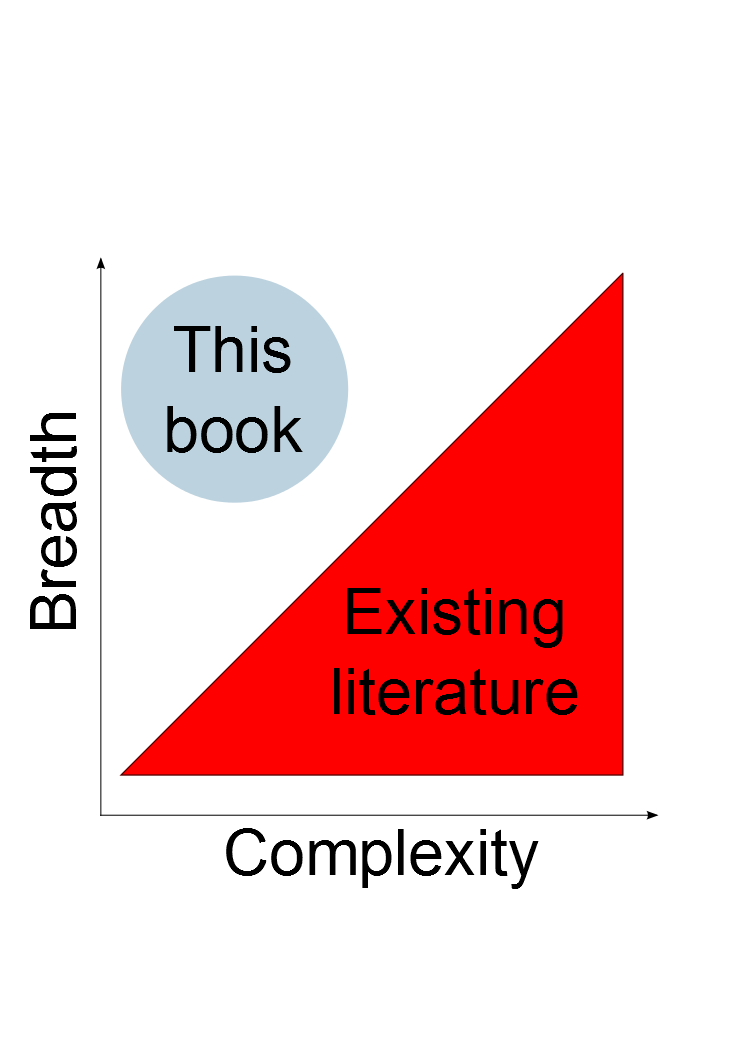
\includegraphics{HowToUse_existingLiterature.png}}
\caption{The aim of this book.}\label{fig:HowToUse_existingLiterature}
\end{figure}


\section{Who is this book for?}
This book is for anyone who has ever tried, and \textbf{failed} at statistics, and particularly, Bayesian statistics.

The text is aimed at anyone who has completed high school mathematics, and wants to conduct Bayesian inference on real world data. We assume no previous knowledge of probability\footnote{Which is central to Bayesian analysis.}, and devote the entirety of chapter \ref{chap:Probability} to this purpose. We do not require that the student is versed in classical statistics, as we aim to build an alternative, and complementary path to a shared goal. As such, after chapter \ref{chap:subjectiveFrequentistBayes}, we will not give too much attention to comparisons between these two approaches.

Whilst we start at the very beginning of statistical inference, we aim to provide a guide which will be of practical-use for a large proportion of analyses that are likely to be encountered in real life.

\section{Pre-requisites}
Knowledge of the following is strongly recommended, in order to allow the reader to grasp all that is contained within this text:

\begin{itemize}
\item \textbf{Algebra:} manipulation of symbolic expressions is widespread throughout the text.
\item \textbf{Summations:} mainly used for writing down likelihood functions.
\item \textbf{Calculus:} mainly integration, although there are sprinklings of differentiation in places.
\end{itemize}

The only other pre-requisite is more to do with the practical application of Bayesian analysis: a knowledge of the statistical software \textit{R}\cite{RLanguage} would be \textit{useful}. We do not classify this item with those above, partly because we aim to only use very basic functioning in this language, and partly because we will explain those examples thoroughly. This language is widely-used for statistical analysis, and because of its popularity there are many excellent online introductions to this language, which are freely available:

\begin{itemize}
\item \url{www.coursera.org} - there are a number of great lecture courses with associated problem sets available for learning R here. In particular, the courses by Roger Peng at John Hopkins are very worthwhile.
\item \url{http://tryr.codeschool.com} - a short interactive introductory lesson on the basics of R. 
\item \url{www.datacamp.com/courses/free-introduction-to-r} - 4 hours of interactive lectures on the basics of R.
\item \url{http://cran.r-project.org/doc/contrib/Owen-TheRGuide.pdf} - a nice written guide to R.
\end{itemize}

Whilst none of these are essential, if you have difficulty in following the examples in this text, then we recommend that you have a look at the above resources.

\section{Book outline}
We have written this text to make each chapter as self-contained as is possible. Whilst, at times, the reader may feel that this focus on modularity means that some elements reoccur, this is intended not to make reading repetitious, or worse \textit{boring}! It is for two purposes: to aid the aforementioned compartmentalisation; and because we believe that some ideas are worth encountering, and re-encountering, at different points in your pursuit of knowledge.

The book is divided into five \textit{Parts}:

\begin{itemize}
\item \textbf{Part} \ref{part:BayesianInferenceIntro}\textbf{: An introduction to Bayesian inference.} 
\item \textbf{Part} \ref{part:bayesianFormula}\textbf{: Understanding the Bayesian formula.}
\item \textbf{Part} \ref{part:analyticalBayes}\textbf{: Analytic Bayesian methods.}
\item \textbf{Part} \ref{part:computationalBayes} \textbf{: A practical guide to doing real life Bayesian analysis: Computational Bayes.}
\item \textbf{Part} \ref{part:regressionHierarchical} \textbf{: Regression analysis and hierarchical models.}
\end{itemize}

Part \ref{part:BayesianInferenceIntro} firstly provides an introduction to the purpose of statistical inference, then goes on to compare and contrast the Bayesian and classical approaches to this problem. Bayesian inference is based on probability. Hence it is imperative to understand how to manipulate these types of mathematical object. The latter half of this part is thus devoted to exactly this purpose. Part \ref{part:bayesianFormula} introduces the reader to the constituent elements of the Bayesian inference formula, and in doing so provides an all-round introduction to the practicalities of doing Bayesian inference. Part \ref{part:analyticalBayes} aims to equip the user with the knowledge of the most practically-relevant probability distributions for Bayesian inference. These objects come under two categories in general\footnote{although some distributions fall into both}: prior distributions, and likelihood distributions. Knowledge of these distributions is essential for understanding existent research papers, and books which use Bayesian statistics, as well as to conduct Bayesian inference in the first place. The rest of the part is concerned with introducing the reader to 'nice' combinations of distributions which allow for a pen-and-paper deduction of quantities of interest. This is important not only as a stepping stone to computational methods, but also because these places are often a good place to start before implementing more nuanced models. Part \ref{part:computationalBayes} introduces the reader to the modern methods of undertaking Bayesian analysis; through computational Markov Chain Monte Carlo. This part aims to provide an intuitive introduction to some of the most important algorithmic tools used in computational methods. It also importantly introduces the reader to the statistical languages covered in this text: \textit{Stan} and \textit{JAGS}. This part is essential reading for anyone wanting to conduct serious real world Bayesian analysis of data. Part \ref{part:regressionHierarchical} builds on the previous part, and introduces the reader to the most important aspect of Bayesian modelling; hierarchical models. It also provides an in-depth introduction to doing Bayesian regression modelling.

Each chapter has two introductory summaries: the \textit{chapter mission statement}, and \textit{chapter goals}. The former is usually a one or two sentence gist of the material to be covered in the following chapter, as well as the learning outcomes of the section. The \textit{chapter goals} section is more detailed, and links together material encountered in previous chapters, and provides more of a narrative on the position of the particular chapter in question in a journey to understand Bayesian statistics. 

The \textit{chapter summary} sections at the end of each chapter provide the reader with a description of the skills acquired within, as well as some perspective on the material's position within the book's overall goals. The \textit{chapter outcomes} section provides a check-list of the skills acquired within the chapter. 

\section{Route planner - suggested journeys through Bayesland}
Ben note to self: \textbf{Change this to make of the same tick and cross table format as that of the Bayesian machine learning book!}

In the style of most good guide books, we provide itineraries through the area in question. These journeys are meant to be shortish paths towards gaining a better understanding of particular elements of Bayesian statistics, although as most trips are, they are not as all-encompassing, as a more prolonged stay. We provide the following trips through Bayesland, based on time, goals, and pre-requisite knowledge:

\begin{itemize}
\item \textbf{The long-weekender (introductory):} chapter \ref{chap:subjectiveFrequentistBayes} introduces you to the theory behind statistical inference, as well as providing a gentle introductory comparison between Bayesian and classical approaches. If you have extra time, and some knowledge of handling probability distributions, then skip ahead to chapter \ref{chap:posterior}.
\item \textbf{The two week basic trip (introductory):} Part \ref{part:BayesianInferenceIntro} and Part \ref{part:bayesianFormula} provide a full introduction to Bayesian statistics, from the ground up. 
\item \textbf{The two week refresher (medium):} Read chapter \ref{chap:subjectiveFrequentistBayes} to get your bearings. Dependent on your knowledge of the Bayesian formula Part \ref{part:bayesianFormula} can either be read, or left behind. Part \ref{part:analyticalBayes} should be read almost in full, as this will get you up to speed with many of the tools necessary to understand many research papers. However, you may be able to 'get away' without reading chapter \ref{chap:ObjectiveBayes} on Objective Bayes.
\item \textbf{The two week full practical swing (medium-master):} If you are happy with your knowledge of the Bayesian inference formula, as well as the distributions used in Bayesian analysis, then you may want to skip ahead to Part \ref{part:computationalBayes}, which introduces computational methods. This introduces the reader to both \textit{Stan} and \textit{JAGS} which are the statistical languages used in this text to carry out Bayesian analyses. If you have time, and are willing, then you may want to progress to Part \ref{part:regressionHierarchical}. 
\item \textbf{The 'I need to do Bayesian analysis' now three day leg (medium-master):} This is a tailor-made trip suited to those practitioners who need to carry out Bayesian data analysis \textit{fast}. The most likely people here are those in research: either academic or corporate; who have an existing knowledge of Bayesian statistics. Skip ahead to Part \ref{part:computationalBayes}, and read the chapter on \textit{Stan} (if your analysis only contains a few discrete variables), or \textit{JAGS} (if your analysis contains a number of discrete parameters). You may then want to use the index to look for the most relevant sections, although Part \ref{part:regressionHierarchical} will be your main point of reference.
\item \textbf{A theoretic and practical journey through modern Bayesian analysis (medium-master):} You want to learn as much about applied Bayesian methods as time will allow, but you also want to gain some practice in practically doing Bayesian statistics. Read all of Part \ref{part:computationalBayes}.
\item \textbf{A two week modelling masterclass (master):} you know all the basics, and are acquainted with the use of either \textit{Stan} or \textit{JAGS\BUGS}. You want to see these applied to carrying out real life data analysis. Read all of Part \ref{part:regressionHierarchical}. 
\end{itemize}

\section{Video}
Whenever the reader sees the following signpost, there is a video available to supplement the main text:

\boxed{Video:}

By following the web address indicated, the user can watch the video on YouTube.

The videos are not meant to replace the reading of the text. They are supplementary, and aim to address topics through alternative approaches, and with different examples.

Ben note to self:\textbf{It might be good to provide a link to a real video here.}

\section{Interactive elements}
Whenever the reader sees the following signpost, there is an interactive element available to supplement the main text:

\boxed{Interactive:}

By following the web address indicated, the user can dynamically interact with these examples, by clicking, entering numbers, or moving slider bars. It is hoped that these elements in particular, will allow the user to build up an intuition behind Bayesian theory, which is essential for doing real world analysis.

These elements have been created using Mathematica, although there is no need to own the software in order to play. 

\section{Interactive problem sets}
The reader can practice their knowledge using the problem sets at the end of each chapter. The problem sets are \textbf{interactive}, and are of the form used in many online education systems. The student can submit their answers to a selection of the questions, and will receive a mark out of 100 for each problem set.

The problems available aim to cover mainly practical application of Bayesian data analysis, although there are also sections which are more theoretic in nature.

For teachers of the subject, there are parts of each problem set which are not interactive, and can be used as a part of a taught course.

\section{Code}
Whenever appropriate, particularly in Part \ref{part:computationalBayes} onwards, we will include snippets of code in Stan, JAGS and R. These are commented thoroughly, which should be self-explanatory. They aim to be as self-contained as space allows.

\section{R, Stan and JAGS}
Modern Bayesian data analysis uses computers. Luckily, for the student of Bayesian statistics, the most up-to-date and useful software packages are open source; meaning they are freely available to use. In this book we solely use this type of software, so prevent the student needing to spend more on acquiring them.

The most recent, and powerful software to emerge is that developed by Andrew Gelman et al.\cite{stan-software:2014} and is called \textit{Stan}. The language of this software is not difficult to understand, and easier to write and debug than its competition. Stan allows a user to fit complex models to data sets, without having to wait an age for the results. With updates planned to this software, which will make it even more powerful, and user-friendly, this is without question the most appropriate software on which to conduct Bayesian analysis.

Ben note to self: Dependent on when the book is released, we may remove the following section, since Stan may allow for discrete sampling directly by then.

The only snag with Stan is that because of the particular type of engine under the hood, it is not possible to directly use it to conduct analysis for discrete parameters. As we shall see in Part \ref{part:computationalBayes}, this issue can be sidestepped in Stan, but for some circumstances it is easier to write the model using another piece of software called \textit{JAGS}\cite{plummer2003jags}. This language is slightly different to write, and in nature to that of Stan. We will explain its functioning in detail in Part \ref{part:computationalBayes}, and walk though a number of introductory examples, however we advocate using this software only in circumstances where it is simpler to implement than a corresponding model in Stan.

The two aforementioned statistical languages are usually run through another piece of 'helper' software. Whilst there are a number of alternatives here, particularly for Stan, we choose to use \textit{R} here. This is because this software is both open source, and widely used. The former means that anyone with a modern computer should be able to get their hands dirty in Bayesian analysis; the latter is important since the code base is well-maintained and tested.

\section{Why don't more people use Bayesian statistics?}
Many are discouraged from using Bayesian approaches to analysis due to its supposed difficulty, and dependence on mathematics. However, we would argue that this is, in part, a weakness of the existent literature on the subject, which this book looks to address. It also highlights how many books on classical statistics sweep their inherent complexity and assumptions under the carpet, resulting in texts which are easy to digest; meaning that for many the path of least resistance is to forge ahead with classical tools. 

By its dependence on the logic of probability, this means on first glances, Bayesian statistics appears more mathematically-complex. However, what is often lost in introductory texts on Bayesian theory, is the intuitive explanations behind the mathematical formulae. In this text instead, we shift the emphasis towards the latter; choosing to focus on graphical and illustrative explanations rather than getting lost in the details of the mathematics, which to be honest, is not necessary for much of modern Bayesian analysis. We hope that by doing so, we shall lose fewer casualties to mathematical complexity, and redress the imbalance between classical and Bayesian analysis applications.

Again, on first appearances, the concept of the \textit{prior} no doubt leads many to 'abandon ship' early on the path to understanding better Bayesian methodologies. However, we will cover this concept in detail in chapter \ref{chap:Prior} which is fully-devoted to this subject, we hope to banish this particular thorn in the side of would-be Bayesian statisticians.

The reliance on computing, in particular simulation, is also seen to add to the complexity of Bayesian approaches. Whilst, this is true, we argue that the modern algorithms used for simulation are straightforward to understand, and with modern software, easy to implement. Furthermore, the added complexity of simulation methods is more than compensated by the straightforward extension of Bayesian models to handle arbitrarily complex situations. Like most things worth learning, there is a slight learning curve to become acquainted with the languages used to write modern Bayesian simulations. However, we hope to make this curve sufficiently shallow by incremental introduction of elements used in these computational applications.

\section{What are the tangible (non-academic) benefits of Bayesian statistics?}
In Bayesian textbooks much discourse is devoted to advocating the academic reasons for choosing to use a Bayesian analysis over classical approaches. However, often authors neglect to promote the more tangible, everyday benefits of the former. Here, we list the following \textit{real} benefits of a Bayesian approach:

\begin{itemize}
\item \textbf{Simple and intuitive model testing and comparison}. The prior- and posterior-predictive distributions allow for in-depth testing of any particular aspect of a model, by comparing it with the same aspects from the data collected. The Bayesian approach also provides a logical framework in which to compare different models.
\item \textbf{Straightforward interpretation of results.} In classical analyses, the \textit{confidence interval} is often taken to be a measure of uncertainty for a particular parameter. As we shall see in section \ref{sec:Posterior_classicalConfidenceInterval}, this is not the case, and interpretation of this concept is not straightforward. By contrast Bayesian \textit{credible intervals}, can be taken to be a measure of uncertainty in a parameter, as they are obtained directly from probability distributions.
\item \textbf{Full model flexibility}. Modern Bayesian analyses use computational simulation in order to carry out analyses. Whilst this might appear excessive when compared to classical approaches, an additional benefit is the straightforward extension to almost arbitrarily complex models when using Bayesian approaches. This means that Bayesian models can be extended to encompass any complexity of data process. This is in contrast to classical approaches, where the intrinsic difficulty of analysis scales with the complexity of the model chosen.
\item \textbf{The best predictions.} Leading figures both inside and outside of academia use Bayesian approaches for prediction. An example being Nate Silver's correct prediction of the 2008 US Presidential election results \cite{silver2012signal}.
\end{itemize}

\section{Suggested further reading}
A good book should leave the reader wanting more. Due to the finiteness of this text, we recommend the following books, articles and websites. These aren't necessarily all on Bayesian statistics, but fall under the wider categories of statistical inference and learning. We also provide a score of the complexity of reading these texts, which may guide your choice:

\begin{itemize}
\item \textbf{Bayesian Data Analysis (medium-master): } A masterpiece produced by the master statisticians Andrew Gelman, and Donald Rubin amongst others. This is the most all-encompassing, and up-to-date text available on applied Bayesian data analysis. There are plenty of examples of Bayesian analysis applied to real world data, and are well-explained\cite{gelman2013bayesian}.
\item \textbf{Data Analysis Using Regression and Multilevel/Hierarchical Models (medium): } Another belter from Andrew Gelman, along with his co-author Jennifer Hill. This takes the reader through numerous examples of regression modelling, and hierarchical analysis. The text is not solely constrained to Bayesian analysis, and covers classical methods as well.
\item \textbf{Mastering metrics (introductory): } A great, back-to-basics, book on causal inference by the masters of econometrics Josh Angrist and Jörn-Steffen Pischke. This is an exhibition of the five main methods used to conduct causal inference in the social sciences: regression, matching, instrumental variables, differences-in-differences, and regression discontinuity design. This is a very readable text, and suitable for anyone wanting to learn about policy evaluation.
\item \textbf{Mostly Harmless Econometrics (master-of-metrics): } Again by Josh Angrist and Jörn-Steffen Pischke. A thorough, and mathematically detailed text which takes the reader through most of those methods used in causal inference today. Its small size is deceptive, and is not one to read over a single weekend. However, it is well worth persisting with this book, as the nuggets that await the determined reader are worth their weight in gold. Also see Gelman's review of this book, which provides an interesting critique of the text.
\end{itemize}

\part{An introduction to Bayesian inference}\label{part:BayesianInferenceIntro}
\section{Part mission statement}
The purpose of this Part is twofold: firstly to introduce the reader to the principles of inference; secondly to familiarise them with knowledge of how to manipulate probability distributions, which is essential to Bayesian inference.

\section{Part goals}
Both Frequentist and Bayesian inferential processes aim to obtain a probability of a hypothesis given the data that was obtained. However, it is much easier to obtain the inverse - the probability of the data given a hypothesis. Thus this process of \textit{inversion} is central to all statistical inference. However, there are two distinct ways to go about inversion: Frequentists use a rule of thumb, which has historically been agreed upon as a useful way of carrying out this process; by contrast Bayesians use Bayes' rule - the only method consistent with the logical of probability. Chapter \ref{chap:subjectiveFrequentistBayes} fully introduces the reader to the aims of statistical inference, along with the differences in philosophy and approach taken by Frequentists and Bayesians to this shared goal. 

One of the main differences in approach is the Bayesian insistence on describing everything of interest using probability distributions. The resultant theory is more elegant, as well as being more practically useful, than that proposed by Frequentists. However, in order to appreciate this elegance, it is necessary to have a good working knowledge of probability distributions, and their manipulations. Hence chapter \ref{chap:Probability} provides a fully introductory course on probability distributions. 

\chapter{The subjective worlds of Frequentist and Bayesian statistics}\label{chap:subjectiveFrequentistBayes}
\section{Chapter mission statement}
At the end of this chapter, the reader will understand the purpose of statistical inference; importantly recognising the similarities and differences between Frequentist and Bayesian inference. We then go on to introduce the most important theorem in modern statistics: \textit{Bayes' rule}.
 
\section{Chapter goals}
In life, we are often tasked with building predictive models to understand complex phenomena. As a first approximation, we often disregard parts of the system, which are not directly of interest; making the models \textit{statistical} rather than deterministic. There are two distinct approaches to statistical modelling: Frequentist or Classical inference, and Bayesian. This chapter will explain the similarities between these two approaches, and importantly, indicate where they differ substantively. It is typically fairly straightforward to calculate the probability of obtaining different data samples, if we assume that we \textit{know} the process that is responsible for generating these data in the first place. However, we normally do not know these processes with certainty, and it is the goal of statistical inference to derive estimates of the unknown characteristics, or \textit{parameters}, of these mechanisms. Bayesian statistics allows us to go from what is known - the \textit{data} - to extrapolate backwards in order to make probabilistic statements about the overriding parameters which were responsible for its generation. This inversion process is carried out in Bayesian statistics by application of Bayes' rule, which will be introduced in this chapter.  It is important to have a good understanding of this rule, and we will spend some time, throughout this chapter and Part \ref{part:bayesianFormula}, developing an understanding the various constituent components of the formula.

\section{Bayes' rule - allowing us to go from the effect back to its cause}\label{sec:Intro_bayesCauseEffect}
Suppose we knew that a casino was crooked, and uses a die with a probability of rolling a 1 that is twice that of its unbiased value. We could then calculate the probability that we roll two 1s in a row:

\begin{equation}\label{eq:Intro_crookedCasinoBayes}
\begin{align}
Pr(1,1) &= \frac{1}{3} \times \frac{1}{3}\\
&= \frac{1}{9}
\end{align}
\end{equation}

Here we use 'Pr' to denote a probability. The probability of $\frac{1}{3}$ is twice that of the unbiased probability: $Pr(1) = 2\times\frac{1}{6} = \frac{1}{3}$. Do not worry if you don't understand fully this calculation, as we will devote the entirety of the next chapter to working with probabilities.

In this case we have presupposed a \textit{cause} - the casino being crooked - in order to derive the probability of a particular effect - rolling two consecutive 1s. In other words we have calculated $Pr(effect|cause)$. The vertical line, $|$, here means \textit{given} in probability\footnote{Again do not worry if you don't understand this notation, as we will devote the entirety of chapter \ref{chap:Probability} to developing an understanding of probability and its notations.}. 

Until the latter half of the 17th Century, probability was most frequently used as a method to calculate gambling odds; similar in nature to that shown in (\ref{eq:Intro_crookedCasinoBayes}). It was viewed as a dirty subject, not worthy of the attention of the most esteemed mathematicians.

However, the arrival of the Reverend Thomas Bayes, and slightly later and more famously, Laplace\footnote{See \cite{mcgrayne2011theory} for an interesting history of Thomas Bayes and Laplace, as well as a history of the use of Bayes' theorem.} started a change in this perspective. They realised that it is possible to move in the opposite direction - to go from effect back to cause:

\begin{equation}
Pr(effect|cause) \xrightarrow{Bayes' theorem} Pr(cause|effect)
\end{equation}

In order to take this leap however, it was necessary to create/discover a rule, which later became known as Bayes' rule\footnote{We use the terms "Bayes' theorem" and "Bayes' rule" interchangeably here.}. This can be written:

\begin{equation}\label{eq:Intro_BayesRuleCauseEffect}
Pr(cause|effect) = \frac{Pr(effect|cause)\times Pr(cause)}{Pr(effect)}
\end{equation}

In the casino example, this formula tells us how to 'invert' the original probability $Pr(1,1|crooked\;casino)$ to get the thing in which we are probably more interested as a patron of said casino $Pr(crooked\;casino|1,1)$. In words, what is the probability that the casino is crooked, \textit{given} that we rolled two 1s. We will not show how to carry out this calculation in practice now; delaying this until we have learned about probability in chapter \ref{chap:Probability}.

Bayes' rule is central to the Bayesian approach to statistical inference. However, before we introduce Bayesian inference, we first need to explain the purpose of inference!

\section{The purpose of statistical inference}\label{sec:Intro_purposeStatisticalInference}
How much does a particular drug contribute to treatment success? What can an average student earn after obtaining a college education? Will the Democrats win the next US Presidential election? In life we often want to test theories, then go on to draw conclusions.

However, it is often impossible to exactly isolate the parts of a system which we want to examine. The outcome of history is hence determined by a nexus of interacting elements; each of which contributes to the reality that we witness. In the case of a drug trial, we may not be able to control the diets of participants, and are certainly unable to control for their idiosyncratic metabolisms, both of which could impact the results we see. Evaluating the return to a college education - there are a range of factors which affect the wage which an individual ultimately commands, of which education is only one element. The outcome of the next US Presidential election depends on party politics, the performance of the incumbent government, as well as the media's portrayal of the candidates. 

In life noise obfuscates the signal. The wind, rain, snow and sleet make it difficult to forge a path to where we want to go.

Statistical inference allows us to draw conclusions in this blustery landscape; separating the signal from the noise. It is the logical framework which we can use to trial our beliefs against \textit{data}. 

In statistics, we formalise our beliefs in models of \textit{probability}. The models are probabilistic because we assume we are ignorant to many of the multitude of interacting parts of a system, meaning we cannot say with certainty whether something will, or will not, occur.

Suppose we are evaluating the efficacy of a drug in a trial. We might suppose that \textit{on average}, the drug might have a given probability of working as desired. However, before we carry out any trials, we are unaware of its exact treatment success rate. Fortunately, statistical inference allows us to estimate this unknown characteristic, or \textit{parameter}, from the data we are given. 

There are two schools of thought for carrying out this process of inference: \textit{Frequentist} and \textit{Bayesian}. Although this book is devoted to the latter, we now spend some time comparing the two approaches, so that a reader is aware of the different paths taken to their shared goal.

\section{The world according to Frequentists}\label{sec:Intro_FrequentistsWorld}
In Frequentist or classical statistics, we suppose that our sample of data is the result of one of an infinite number of exactly-repeated experiments. The sample we see in this context is hence assumed to be the outcome of some probabilistic process. Any conclusions that we draw from this approach are based on the supposition that events occur with probabilities, which represent long-run frequencies. 

For example, if we flip a coin, we might assume that any sequence of outcomes we obtain is indicative of results we'd get if we were to conduct the experiment an infinite number of times. Further, we might take the proportion of heads observed in this infinite set of throws as defining the probability of obtaining a 'heads'. We suppose that this probability actually exists, and is fixed for each set of coin-throws that we carry out (see figure \ref{fig:Intro_FrequentistBayesProbability}).

In general, in Frequentist statistics assume that the data is \textit{random} and results from \textit{sampling}, from a fixed and defined \textit{population} distribution. For a Frequentist the noise that obscures the true signal of the population relationship in which we are interested is due to \textit{sampling variation}; the fact that the sample that we pick will each time be slightly different, and not exactly representative of the population. 

We may flip our coin 10 times, obtaining 7 heads even if the long-run proportion of heads is $\frac{1}{2}$. To a Frequentist, this is because we have picked a slightly odd sample from the population of infinitely-many repeated throws. Further, if we flip the coin another 10 times, we will likely get a different result, because we have picked a different sample.

\begin{figure}
\centering
\scalebox{0.3} 
{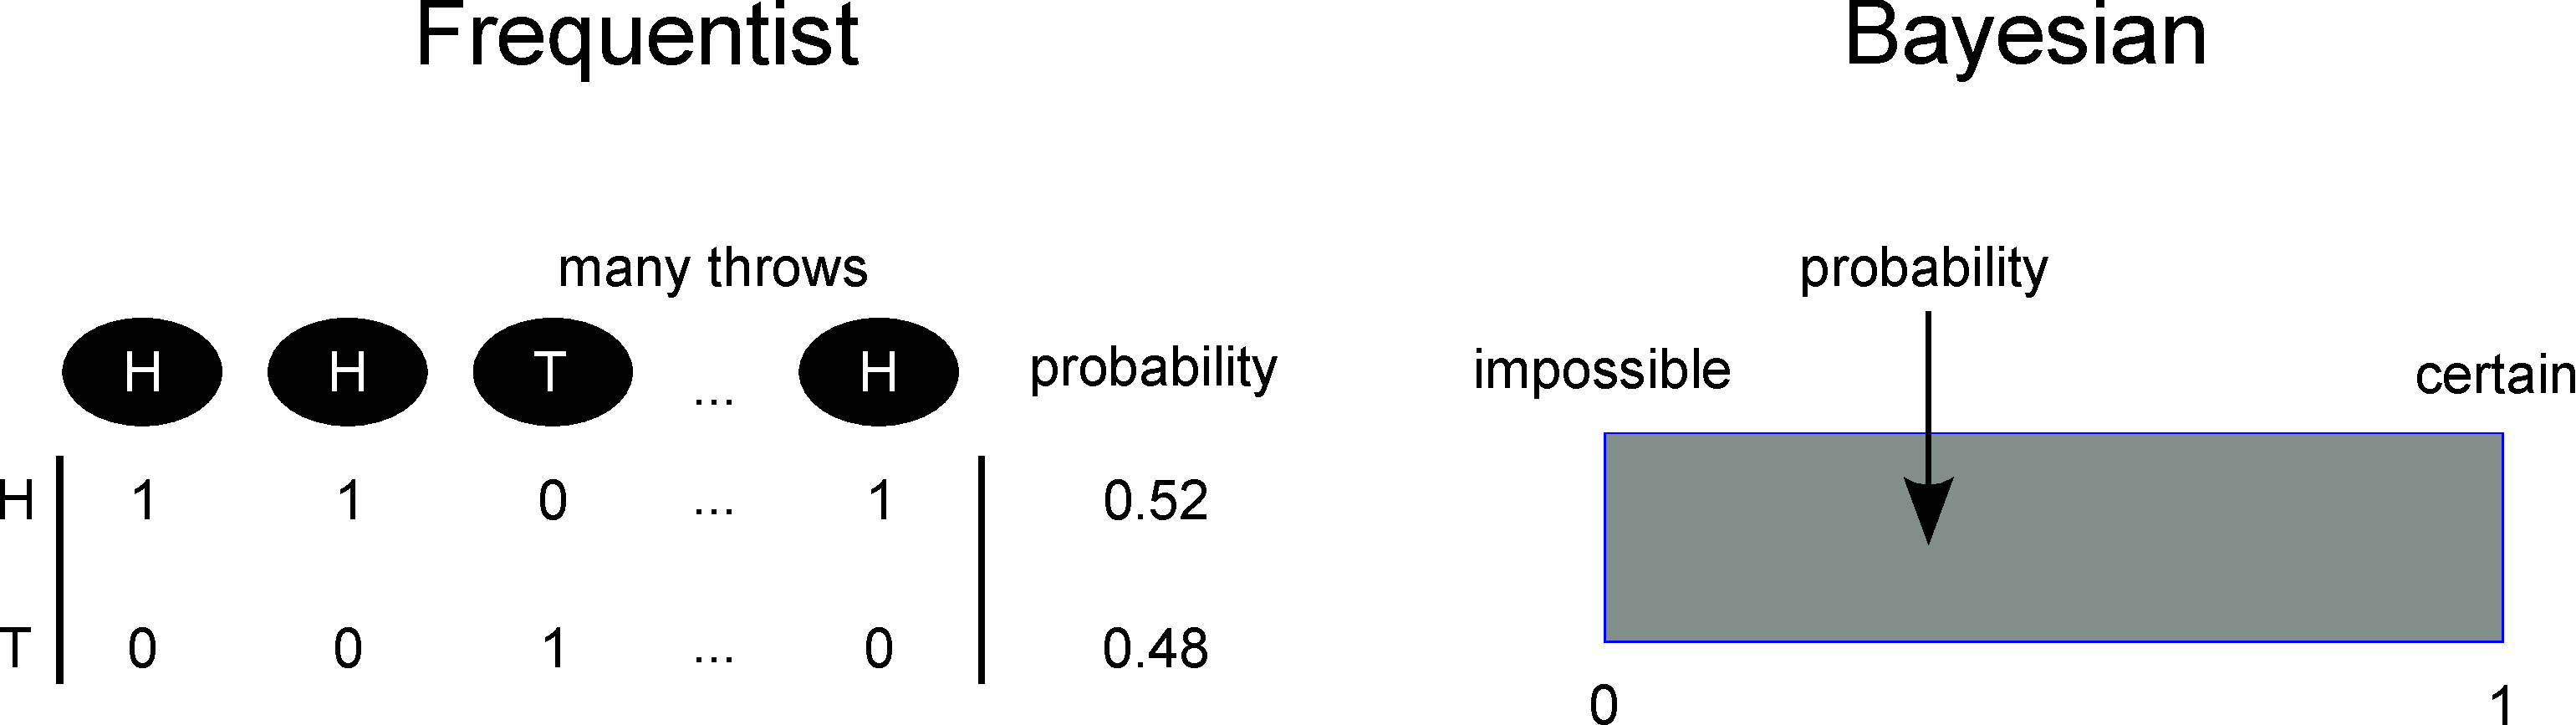
\includegraphics{Intro_FrequentistBayesProbability.pdf}}
\caption{The Frequentist and Bayesian approaches to probability.}\label{fig:Intro_FrequentistBayesProbability}
\end{figure}

\section{The world according to Bayesians}
Bayesians do not imagine repetitions of an experiment in order to define and specify a probability. It is merely taken as a measure of certainty of a particular belief. From this viewpoint, the probability of us throwing a 'heads' measures and quantifies our underlying belief, that before we flip the coin, it will land this way. 

In this sense, Bayesians do not view probabilities as concrete entities that actually exist. They are merely abstractions which we can use to help express our uncertainty. In this frame of reference there is no necessity for events to be repeatable in order to define a probability. We are thus equally able to say, 'The probability of a heads is 0.5', or, 'The probability of the democrats winning the 2020 US Presidential election is 0.75'. Probability is merely seen as a scale from: 0 where we are certain an event will not happen, to 1 where we are certain it will (see figure \ref{fig:Intro_FrequentistBayesProbability}). 

A statement such as 'The probability of the democrats winning the 2020 US Presidential election is 0.75' is hard to explain using the Frequentist definition of a probability. There is only ever one possible sample - the history that we witness - and what would we actually mean by a 'population of all possible US elections which happen in the year 2020'? 

Probabilities are therefore seen as an expression of subjective beliefs, meaning they can be updated in light of new data. The formula invented by the Reverend Thomas Bayes provides the \textit{only} logical manner in which to carry out this process, and is central to Bayesian inference, where we aim to express probabilistically our uncertainty in parameters after we have seen the \textit{data}. 

Bayesians assume, since we are witness to the data, that it is \textit{fixed}, and therefore does not vary. We do not need to imagine that there are an infinite number of possible samples. We 'see' our data, and hence do not need to view it as the outcome of some random process.

In contrast, we do not ever learn exactly the value of an unknown parameter. This epistemic uncertainty means that in Bayesian inference we choose to view the parameter as a quantity that is probabilistic in nature. We can view this in one of two perspectives. Either we view the unknown parameter as truly being \textit{fixed} in some absolute sense, but our beliefs are uncertain, and thus probabilistic. Alternatively, we can take the view that there isn't some definitive \textit{population} process, and for each sample we take, we get a slightly different parameter.

In the latter perspective we get different results from the coin flipping because each time we are subjecting our system to a slightly different probability of it landing 'heads' up. This could be because we mildly altered our throwing technique, or started with the coin in a different position. In the former perspective, we view the sample as a noisy representation of the signal, and hence we get different results for each set of throws. Although these two descriptions are different philosophically, they are not mathematically, meaning we can apply the same analysis to both.

\section{Frequentist and Bayesian inference}
The Bayesian inference process is the only logical way to modify our beliefs to take into account new data. We start out before we collect data with a probabilistic description of our beliefs, which we call a \textit{prior}. We then collect data, and together with a model describing our theory, Bayes' formula for probability allows us to calculate our post-data or \textit{posterior} belief:

\begin{equation}
prior + data \xrightarrow{model} posterior
\end{equation}

Ignore for the moment that we have not explained was is meant by this mysterious \textit{prior}, as we shall introduce this element properly in section \ref{sec:Intro_priors}. 

In Bayesian inference, we want to draw conclusions based on purely probabilistic descriptions of phenomena. If we wish to summarise our evidence for a particular hypothesis, we describe this probabilistically, as the 'probability of the hypothesis \textit{given} the data obtained'. 

The difficulty in obtaining this type of conclusion is that when we write down a probability model describing the situation under examination, we can only use it to compute the 'probability of obtaining our data \textit{given} our hypothesis being true'; the inverse of that which we desire. This probability is calculated by taking into account all the possible samples that we could have obtained from the population, if we assume the hypothesis is true. The issue of statistical inference, common to both Frequentists and Bayesians, is to how to invert this probability to get the desired quantity of interest.

Frequentists stop here, using this probability as evidence for a particular hypothesis in question. If the probability of obtaining the data, or a data sample more extreme, given a hypothesis is small, then it is assumed that it is unlikely that the hypothesis is true, and is rejected. Note however if reject a hypothesis, we have no way of telling whether it is true, and we just witnessed a weird sample, or that it is actually false. Also, note that in this inference process, we have also had to imagine obtaining a sample more extreme than our result, in order to get a usable probability. 

Bayes' formula allows us to circumvent these difficulties, by inverting the Frequentist probability to get the 'probability of the hypothesis given the \textit{actual} data we obtained'. There is no need for an arbitrary cut-off in the probability in order to validate the hypothesis; all information is summarised in this probability, and hence can be viewed as the end point of an analysis in itself.

\begin{figure}
\centering
\scalebox{0.4} 
{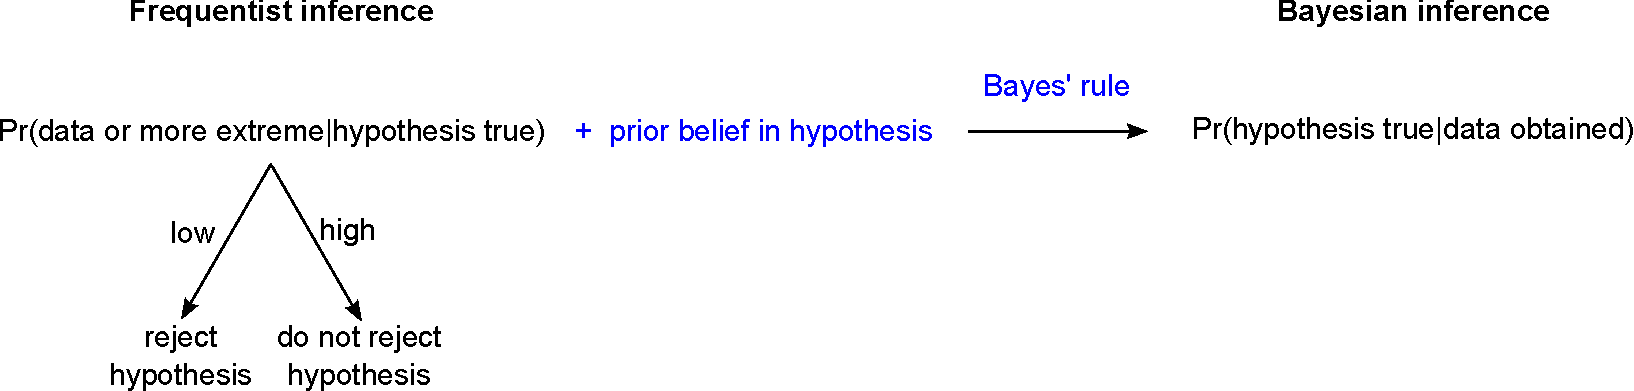
\includegraphics{Intro_BayesVsFrequentist.pdf}}
\caption{Frequentist and Bayesian inference.}\label{fig:Intro_BayesVsFrequentist}
\end{figure}

The next few, albeit silly, and (more than) somewhat contrived examples, illustrate a difference both in methodology, but perhaps more significantly, in philosophy, between the two different approaches.

\subsection{The Frequentist and Bayesian murder trials}
Assume you find yourself in the unfortunate situation where you are (hopefully falsely) accused of murder, and face a trial by jury. A variation in the usual tale is that you personally have a choice over the method used by the jury to assign guilt: either Frequentist or Bayesian. Another unfortunate twist is that the legal system of the country starts by presuming \textit{guilt} rather than \textit{innocence}.

Let's assume that you have been shown by a security camera to have definitely been in the same house as the victim - Sally - on the night of her demise. 

If you choose the Frequentist trial, your jurors start by coming up with a model based on previous trials, which assigns a probability of you being seen by the security camera if you were guilty. They then use this to make the statement that, 'If you did commit the murder, then 30\% of the time you would have been seen by the security camera', based on a hypothetical infinity of repetitions of the same conditions. Since this is not sufficiently unlikely (the p value is not below 5\%), the jurors cannot reject the null hypothesis of \textit{guilt}, and you are sentenced to life in prison.

In a Bayesian trial, the jury are first introduced to an array of evidence, that suggests that you neither knew Sally, nor had any previous record of violent conduct; being otherwise a perfectly respectable citizen. Furthermore, the ex-boyfriend of Sally is a multiple-violent-offending convict on the run from prison after being sentenced by a judge on the basis of witness testimony by Sally. On this basis, the jury determine a \textit{prior} probability in the hypothesis that you are guilty that is $\frac{1}{1000}$\footnote{Do not worry that we are yet to explain how one can construct priors, since we shall devote the entirety of chapter \ref{chap:Prior} to this purpose.}. They then use the same model as the Frequentists, to determine that the probability of you being seen by the security camera given your guilt is 30\%. However, they then coolly use Bayes' rule\footnote{We will introduce this concept in section \ref{sec:Intro_bayesCauseEffect}.}, and conclude that the probability of you committing the crime is $\frac{1}{1000}$ (see section \ref{sec:Intro_appendixMurder} for a full description of this calculation). Based on this evidence, the jury acquits you, and you go home to your family.

\subsection{Radio control towers: example}
In a hypothetical war two radio control workers sit side-by-side, Mr Pearson (from frequentland), and Mr Laplace (from the county of Bayesdom), and are tasked with finding an enemy plane that has been spotted over the country's borders. They will each feed this information to the nearest airforce base(s) which will respond by sending up aircraft of their own. There are however, administratively two different airforces, which correspond to the two different counties. Although the airforces of frequentland and Bayesdom share airbases, they are distinct, and only respond to Mr Pearson and Mr Laplace's advice respectively. The war, although short, has been costly to both allies, and they each want to avoid needless expenditure, as well as the unwarranted scaring of the local populace by sending up jets.

Mr Pearson starts by inputting the radar information into a computer program which uses a model of a plane's position which has been calibrated against a dataset of historical plane data in this short war. The result comes out instantly. 

"...The plane is most likely 5 miles from the town of Tunbridge Wells."

Without another moment's thought, Mr Pearson radios the base of Tunbridge Wells, telling them to scramble all 10 available Frequentist fighter jets immediately. He then gets up to get himself a well-earned coffee.

Laplace knows from experience there are three different flight paths that the enemy has used to attack previously. Accordingly, he gives these regions a high probability density in his prior for the plane's current location, and feeds this into the same computer program that Pearson used. The output this time is different. By using the optional input, the program now outputs a map with the most likely regions shown via a colour shading. There is the highest posterior density over the region near Tunbridge Wells, where Pearson radioed, although the map suggests there are two other towns which might be likely victims of the plane's bombing. Accordingly, Laplace radios to Tunbridge Wells, asking them to send up four jets, and to the other two towns, asking them to send up two jets each. At the end of this all, Laplace remains seated, tired but contented that he has done his best for his own.

The enemy bomber turned out to be approaching Berkstad, one of the towns which Laplace radioed. The Bayesdom jets intercept the encroaching aircraft, and escort it out of allied airspace. Laplace is awarded a medal in honour of his efforts. Pearson looks on jealously.

\section{Bayesian inference via Bayes' rule}
Bayes' rule tells us how to update our prior beliefs in order to derive better, more informed beliefs about a situation in light of new data. As was explained in section \ref{sec:Intro_purposeStatisticalInference}, statistical inference is concerned with estimating characteristics of interest, which we call \textit{parameters}, from a dataset that we have to hand. From this point onwards we will use, $\theta$, to represent the unknown parameter(s) which we are interested in estimating. 

The Bayesian inference process uses Bayes' rule to estimate a probability distribution over those unknown parameters, after we witness the data. Do not worry if you do not know what is meant by a \textit{probability distribution}, since we shall devote the entirety of chapter \ref{chap:Probability} to this purpose. However, it is sufficient for now to describe probability distributions as a way of representing uncertainty over unknown quantities.

The form of Bayes' rule used in statistical inference is of the form:

\begin{equation}\label{eq:Intro_bayesianFormula}
p(\theta|data) = \frac{p(data|\theta)\times p(\theta)}{p(data)}
\end{equation}

Here we use $p$ to indicate a probability distribution which may either represent probabilities, or more usually, probability densities\footnote{See section \ref{sec:Probability_densityVsMassFunctions} for a description of their distinction.}. We shall now devote the next few sections to describing, in short, the various elements of (\ref{eq:Intro_bayesianFormula}). Note these only provide a partial introduction, since we will spend the entirety of Part \ref{part:bayesianFormula} to an extensive discussion of each of its constituent components.

\subsection{Likelihoods}\label{sec:Intro_likelihoods}
Starting with the numerator on the right hand side of (\ref{eq:Intro_bayesianFormula}), we come across the term $p(data|\theta)$, which we call the \textit{likelihood}. This tells us the probability of generating the particular sample of \textit{data}, if the parameters in our statistical model were equal to $\theta$. When we write down a statistical model, we can generally calculate the probability of particular outcomes, so this is easily obtained. Imagine that we have a coin that we believe to be fair. By \textit{fair}, we typically mean that the probability of the coin falling 'heads-up' is $\theta=\frac{1}{2}$. If we flip the coin twice, we might suppose that it is reasonable to model the outcomes as independent (see section \ref{sec:Probability_independence}), and hence we can calculate the probabilities of the four possible outcomes, by multiplying the probabilities of the individual outcomes together:

\begin{equation}
\begin{align}
p(HH) &= p(H)\times p(H) = \frac{1}{2} \times \frac{1}{2} = \frac{1}{4}\\
p(HT) &= p(H)\times p(T) = \frac{1}{2} \times \frac{1}{2} = \frac{1}{4}\\
p(TH) &= p(T)\times p(H) = \frac{1}{2} \times \frac{1}{2} = \frac{1}{4}\\
p(TT) &= p(H)\times p(H) = \frac{1}{2} \times \frac{1}{2} = \frac{1}{4}\\
\end{align}
\end{equation}

Hence, if we obtained a \textit{sample} of two heads, we could write down the corresponding likelihood, $p(HH|\theta=\frac{1}{2})=\frac{1}{4}$.

Do not worry if you do not fully understand this concept, as we will be devoting an entire chapter to likelihoods in chapter \ref{chap:Likelihoods}.

\subsection{Priors}\label{sec:Intro_priors}
The next term in the numerator of the right hand side, $p(\theta)$ is the most controversial\footnote{Although this controversy is unwarranted, as we explain in section \ref{sec:Intro_implicitExplicitSubjectivity}.} part of the Bayesian formula, which we call the \textit{prior} distribution of $\theta$. It is a probability distribution which represents our pre-data beliefs as to the likely values of the parameters in our model, $\theta$. This appears at first to be slightly counter-intuitive, particularly if you are used to the world of classical statistics, which does not require us to state our beliefs \textit{explicitly}\footnote{Although, we always do \textit{implicitly}, as we explain in section \ref{sec:Intro_implicitExplicitSubjectivity}.}. Continuing the coin example, we might assume that we do not know whether the coin is fair or biased beforehand, so we might think that all possible values of $\theta\in[0,1]$ - which represents the probability of the coin falling 'heads-up' - are equally likely. We might represent these beliefs by a continuous uniform probability density on this interval (see the left-hand graph of figure \ref{fig:Intro_priors}). Normally however, we might think that coins are manufactured such that the weight distribution is fairly symmetrical on either face; meaning that we expect that the majority of coins are reasonably fair. These latter beliefs of unbiasedness might be fairly well represented by the right-hand graph of figure \ref{fig:Intro_priors}.

\begin{figure}
\centering
\scalebox{0.6} 
{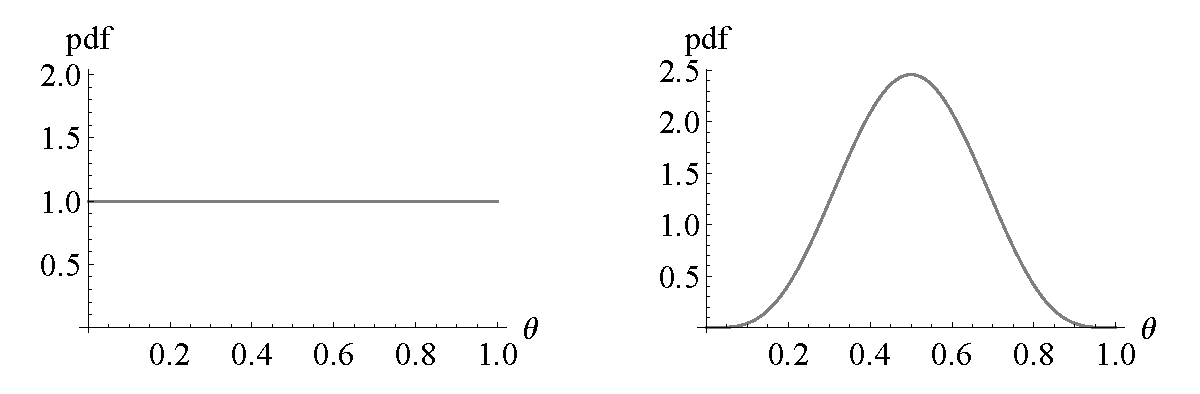
\includegraphics{Intro_priors.pdf}}
\caption{Left: All values of a the bias of a coin are equally likely. Right: It is believed that the coin is most likely fair.}\label{fig:Intro_priors}
\end{figure}

The concept of \textit{priors} will be covered in detail in chapter \ref{chap:Prior}.

\subsection{The denominator}
The final term on the right hand side, on the denominator is $p(data)$. This represents the probability of obtaining our particular sample of data, if we assume a particular model and prior. We will mostly postpone further discussion of this term until chapter \ref{chap:denominator}, when we understand better the significance of \textit{likelihoods} and \textit{priors} respectively. However, for our purposes here it suffices to say that the denominator is fully determined by choice of prior and likelihood function. Whilst it appears simple, this is deceptive, and it is partly the difficulty with calculating this term directly that leads to the introduction of computational methods of the form we will encounter in Part \ref{part:computationalBayes}.

The concept of \textit{the denominator} will be covered in detail in chapter \ref{chap:denominator}.

\subsection{Posteriors: the goal of Bayesian inference}
The posterior probability distribution $p(\theta|data)$ is often the main goal of Bayesian inference. For example, we might want to derive a probability distribution representing our post-experimental beliefs of the inherent bias, $\theta$, of a coin, \textit{given} that we flipped it 10 times, and it came up 'heads' 7 times. If we use (\ref{eq:Intro_bayesianFormula}), assuming the likelihood model specified in section \ref{sec:Intro_likelihoods} and the flat uniform prior shown in figure \ref{fig:Intro_priors}, then we would end up with a posterior distribution shown in figure \ref{fig:Intro_posterior}. Notice that the peak of the distribution occurs at $\theta=0.7$, which corresponds exactly with the percentage of 'heads' seen in the experiment\footnote{Note that if we chose a non-uniform prior, this peak would most likely shift.}. 

\begin{figure}
\centering
\scalebox{0.6} 
{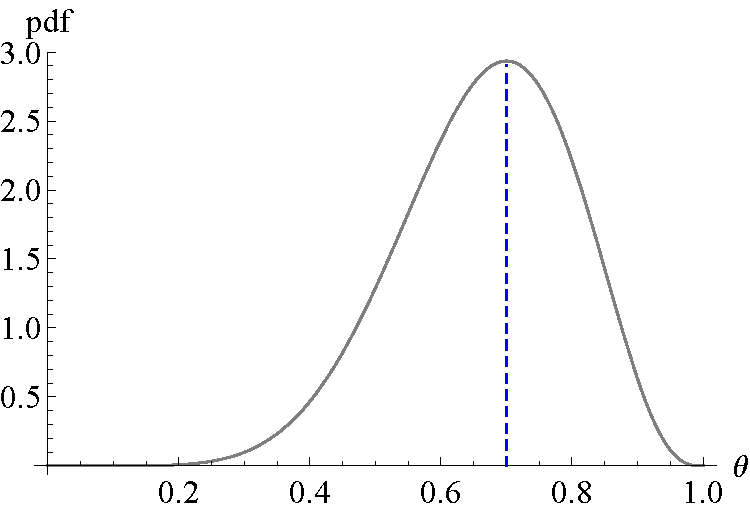
\includegraphics{Intro_posterior.pdf}}
\caption{The posterior distribution for, $\theta$, the bias of a coin when flipped, assuming a flat uniform prior and Bernoulli likelihood. We assume that 7/10 times the coin came up 'heads'.}\label{fig:Intro_posterior}
\end{figure}

The posterior distribution summarises our uncertainty regarding the value of a parameter. If the distribution is more peaked, then this emphasises that there is a greater degree of certainty with a particular value for a parameter. This increased certainty over a parameter value is frequently obtained by collecting more data. In figure \ref{fig:Intro_posteriorPeaked}, we compare the posterior distribution for the previous case of 7/10 times a coin appearing 'heads' up, with a new, larger, sample where 70/100 times the same coin comes up 'heads'. In both cases the same ratio of 'heads' to 'tails' appeared, resulting in the same peak value of $\theta=0.7$. However, in the latter case, since we have more evidence to support our claim, we end up with greater certainty over the parameter value after the experiment.

\begin{figure}
\centering
\scalebox{0.6} 
{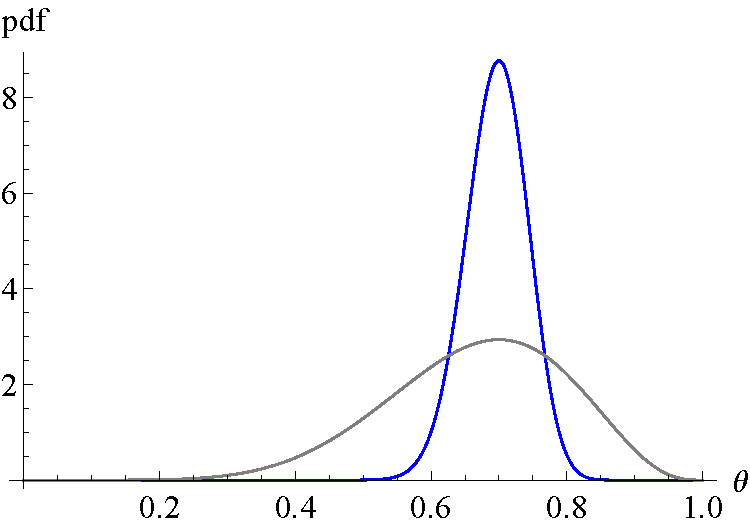
\includegraphics{Intro_posteriorPeaked.pdf}}
\caption{Posterior distributions for, $\theta$, the bias of a coin when flipped, assuming a flat uniform prior and Bernoulli likelihood. The grey line assumes that 7/10 times the coin came up 'heads'. The blue line is for the case where 70/100 times the coin came up 'heads'.}\label{fig:Intro_posteriorPeaked}
\end{figure}

The posterior distribution is also used as a starting point for prediction of future outcomes of an experiment, as well as for model testing. However, we will leave discussion of these until chapter \ref{chap:posterior}.

\section{Implicit vs Explicit subjectivity}\label{sec:Intro_implicitExplicitSubjectivity}
One of the major arguments levied against Bayesian statistics is that it is by its nature \textit{subjective}, due to its dependence on the analyst specifying their pre-experimental beliefs through \textit{priors}. This experimenter prejudice towards certain outcomes is said to bias the results away from the types of fair, objective outcomes resultant from a classical analysis. 

We argue that \textit{all} analyses involve a degree of subjectivity, which is \textit{implicitly} assumed. In a classical analysis, the statistician typically states a model for probability which depends on a range of assumptions,  should be justified explicitly. This process of justification is indicative of the subjective nature of the assumptions on which most analyses rest. For example, the choice to use a simple \textit{linear regression model} in many applied classical analyses assumes that the response of a dependent variable is linear in the model's parameters. This choice of model architecture is generally arbitrary, and used mostly to simplify the analysis. 

In science, there is a tendency amongst scientists to use data to suit one's needs, although this practice should really be discouraged (see \cite{ioannidis2005most}). This choice as to which data points to include is subjective, and will remain independent of the type of analysis applied. 

A further source of subjectivity is in the way in which models are checked and tested. In analyses, both classical and Bayesian, there is a need to exercise (subjective) judgement in suggesting a methodology which will be used in this process. We would argue that a Bayesian analysis allows greater flexibility, and suitable methodologies for these processes, since the prior- and posterior- predictive distributions are straightforwardly manipulated to suit most situations. A Bayesian methodology also allows different models to be compared in a logically-coherent manner, whilst classical analysis relies on fairly arbitrary criteria \footnote{$\bar{R^2}$, AIC and BIC are examples} to do so.

In contrast to the examples of \textit{subjectivity} which we have mentioned above, Bayesian \textit{priors} are \textit{explicitly} stated. This makes this part of the analysis openly available to the reader, allowing it to be as thoroughly interrogated and debated, as any part of an argument. This transparent nature of Bayesian statistics has lead many to suggest that it is \textit{honest}; whilst classical analyses hide behind a fake veil of \textit{objectivity}, Bayesian equivalents explicitly acknowledge the subjective nature of knowledge.

Furthermore, the more data that is collected, the less impact the prior exerts on posterior distributions. In any case, if slight modification to priors results in a different conclusion being reached, it is the job of the researcher to report this sensitivity. In fact, in contrast to classical analyses, a Bayesian analysis allows for a range of models/priors to be stated, which can then be used to test the sensitivity of conclusions to any subjective assumptions made.

Finally, comparing the classical and Bayesian approach to pursuit of knowledge, we find two different solutions; both of which require a subjective judgement to be made. In both cases we would like to have access $p(\theta|data)$ - the probability of the parameter/hypothesis of interest after we have obtained a given data set. In classical hypothesis testing we do not calculate this quantity directly, but use a rule of thumb: we calculate the probability that the data would have been more extreme than that which we obtained under a 'null hypothesis'. If the probability is sufficiently small, typically less than a cut-off of 5\% or 1\%, then we reject the null. Note that this choice of threshold probability - known as a statistical test's \textit{size} - is completely \textit{arbitrary}, and subjective. In Bayesian statistics, we instead use a prior to invert the likelihood from $p(data|\theta)\rightarrow p(\theta|data)$. There is no need to have a null hypothesis and an alternative, since all information is summarised neatly in the posterior. In this way we see a symmetry in the choice of classical \textit{size} and Bayesian priors; they are both attempts to invert the likelihood to get a posterior. 

\section{Chapter summary}
This chapter has focused on the philosophy of inference processes in general, and in particular on the philosophical differences between Bayesian and Frequentist inference. We then introduced the Bayesian formula, and provided a short introduction to its constituent parts. The Bayesian formula is the central dogma of Bayesian inference. However, in order to use this rule for statistical analyses, it is necessary to understand and more importantly, be able to manipulate, probability distributions. The next chapter is devoted to this cause.

\section{Chapter outcomes}
The reader should now be familiar with the following concepts:

\begin{enumerate}
\item The goals of statistical inference.
\item The difference in interpretation of probabilities for Frequentists vs Bayesians.
\item The differences in inferential approaches for Frequentists vs Bayesians.
\end{enumerate}

\section{Problem set}
\subsection{The deterministic nature of random coin throwing.}
Suppose that in an idealised world, the ultimate fate of a thrown coin - heads or tails - is deterministically given by: the angle at which you throw the coin, and the height above a table. Also, in this ideal world, the heights and angles are discrete. However, the system is chaotic\footnote{Highly sensitive to initial conditions.}, and the results of throwing a coin at a given angle and height are shown in table \ref{tab:Intro_PS_coinThrowsDeterministic}. 

\begin{table}[htbp]
  \centering
    \begin{tabular}{rccccc}
    \toprule
          & \multicolumn{5}{c}{\textbf{Height above table (m)}} \\
    \midrule
    \multicolumn{1}{c}{\textbf{Angle}} & \textbf{0.2} & \textbf{0.4} & \textbf{0.6} & \textbf{0.8} & \textbf{1} \\
    \multicolumn{1}{c}{\textbf{0}} & T     & H     & T     & T     & H \\
    \multicolumn{1}{c}{\textbf{45}} & H     & T     & T     & T     & T \\
    \multicolumn{1}{c}{\textbf{90}} & H     & H     & T     & T     & H \\
    \multicolumn{1}{c}{\textbf{135}} & H     & H     & T     & H     & T \\
    \multicolumn{1}{c}{\textbf{180}} & H     & H     & T     & H     & H \\
    \multicolumn{1}{c}{\textbf{225}} & H     & T     & H     & T     & T \\
    \multicolumn{1}{c}{\textbf{270}} & H     & T     & T     & T     & H \\
    \multicolumn{1}{c}{\textbf{315}} & T     & H     & H     & T     & T \\
    \bottomrule
    \end{tabular}%
  \caption{The results of a coin throw from a given angle and height above a table.}\label{tab:Intro_PS_coinThrowsDeterministic}%
\end{table}%

\subsubsection{Suppose that all combinations of angles and heights are equally likely to be chosen. What is the probability that the coin lands on heads?}

Now suppose that the some combinations of angles and heights are more likely to be chosen than others, with the probabilities seen in table \ref{tab:Intro_PS_coinThrowsFrequency}. 

\subsubsection{What are the new probabilities that the coin lands heads-up?}
\subsubsection{Suppose we force the coin-thrower to throw the coin at an angle of 45 degrees. What is the probability that the coin lands heads-up?}
\subsubsection{Suppose we force the coin-thrower to throw the coin at a height of 0.2m. What is the probability that the coin lands heads-up?}
\subsubsection{If we constrained the angle and height to be fixed, what would happen in repetitions of the same experiment?}
\subsubsection{In light of the previous question, comment on the Frequentist assumption of \textit{exact repetitions} of a given experiment.}

\begin{table}[htbp]
  \centering
    \begin{tabular}{cccccc}
    \toprule
    \textbf{Angle} & \textbf{0.2} & \textbf{0.4} & \textbf{0.6} & \textbf{0.8} & \textbf{1} \\
    \midrule
    \textbf{0} & 0.05  & 0.03  & 0.02  & 0.04  & 0.04 \\
    \textbf{45} & 0.03  & 0.02  & 0.01  & 0.05  & 0.02 \\
    \textbf{90} & 0.05  & 0.03  & 0.00  & 0.03  & 0.02 \\
    \textbf{135} & 0.02  & 0.03  & 0.04  & 0.00  & 0.04 \\
    \textbf{180} & 0.03  & 0.02  & 0.02  & 0.00  & 0.03 \\
    \textbf{225} & 0.00  & 0.01  & 0.04  & 0.03  & 0.02 \\
    \textbf{270} & 0.03  & 0.00  & 0.03  & 0.01  & 0.04 \\
    \textbf{315} & 0.02  & 0.03  & 0.03  & 0.02  & 0.01 \\
    \bottomrule
    \end{tabular}%
  \caption{The probability that a given person throws a coin at a particular angle, and at a certain height above a table.}\label{tab:Intro_PS_coinThrowsFrequency}%
\end{table}%


\subsection{Model choice}
Suppose that you have been given the data contained in "Intro\_PS\_overfitShort.csv", and are asked to find a 'good' statistical model to fit the $(x,y)$ data.

\subsubsection{Fit a linear regression model using classical least squares. How reasonable is the fit?}
\subsubsection{Fit a quintic (powers up to the 5th) model to the data. How does its fit compare to that of the linear model?}

You are now given new data contained within "Intro\_PS\_overfitLong.csv". This contains data on 1000 replications of the same experiment, where the $x$ values are held fixed.

\subsubsection{Fit a linear regression to each of the data sets, and similarly for the quintic model. Which of these performs best?}

\subsubsection{Using the fits from the first part of this question, compare the performance of the linear regression model, with that of the quintic model.}
Hint: do not re-estimate the model with new datasets.

\subsubsection{Which of the two models do you prefer, and why?}
\subsubsection{If you then found out that the data were years of education (x), and salary in \$000s (y). Which model would you favour?}

\section{Appendix}
\subsection{The Frequentist and Bayesian murder trial}\label{sec:Intro_appendixMurder}
In the Bayesian trial the probability that you are guilty given being seen by the security camera on the night of the murder is:

\begin{equation}\label{eq:Intro_murder}
\begin{align}
p(guilt|security\; camera footage) &= \frac{p(security\; camera footage|guilt)\times p(guilt)}{p(security\; camera footage)}\\
&= \frac{\frac{30}{100}\times \frac{1}{1000}}{\frac{30}{100}\times \frac{999}{1000}+\frac{30}{100}\times \frac{1}{1000}}\\
&\approx \frac{1}{1000}
\end{align}
\end{equation}

In (\ref{eq:Intro_murder}) we have implicitly assumed that the security camera is hidden, and hence the murderer does not alter his behaviour to avoid being seen; meaning that the probability of being seen by the security camera in each case is 30\%. 

\chapter{Probability - the nuts and bolts of Bayesian inference}\label{chap:Probability}
\section{Chapter mission statement}
Bayesian statistics formulates models in terms of entities called \textit{probability distributions}. This chapter provides an introduction to all things related to probability; starting at interpretation, and allowing the reader to gain an understanding of how to manipulate these distributions.

\section{Chapter goals}
The logical way to express uncertainty in one's beliefs is through probability distributions, and hence Bayesians aim to derive these as goals of the inferential process. Bayesian inference begins with the prior probability distribution expressing our pre-study beliefs. Bayes' rule then tells us how to update these beliefs in light of data, to produce an updated set of beliefs that we call a \textit{posterior} probability distribution. All information of interest is contained within this latter probability distribution, and are the starting point for making decisions based on the statistical analysis. This chapter takes a step away from Bayesian inference to focus on probability distributions; assuming no previous knowledge of them. In order to understand these abstract objects, we shall first devote some time to explicitly define what is meant by probability distributions. This exercise is also useful since Bayesian inference is based on attempts to invert the \textit{likelihood} to get a proper probability distribution. We will also discuss why the distinction between a likelihoods and probabilities is important. We then explain how to manipulate probability distributions in order to derive quantities of interest; starting with simple 1-dimensional distributions, and working up to more adventurous examples, typical of the variety encountered in Bayesian inference. We finish with a derivation of the Bayesian formula from the law of conditional probability. 


\section{Probability distributions: helping us explicitly state our ignorance}\label{sec:Probability_probabilityDistributions}
Before we look out the window in the morning, before we get our exam results, before the cards are dealt, we are uncertain of the world that lies in wait of us. In order to plan, as well as make sense of things, we often predict the relative likelihood of different outcomes. However, in order to allow interrogation of thought, with a view to transparency and self-improvement, we sometimes would like to state our pre-conceptions \textit{explicitly}, using a suitable framework. 

The mathematical theory of probability provides a logic and language which is suitable to describe the majority of cases in which we are uncertain. Imagine that we enter a lottery, where we select a number from 1-100, to have a chance of winning \$1000. We suppose that in the lottery only one ball is drawn, and it is fair with all numbers being equally likely to win. Although we haven't stated this world-view in mathematical notation, we have without realising it, formulated a valid probability distribution for the number drawn in the lottery (see \ref{fig:Probability_lotterySecondhandCarProbability}).

\begin{figure}
\centering
\scalebox{0.3} 
{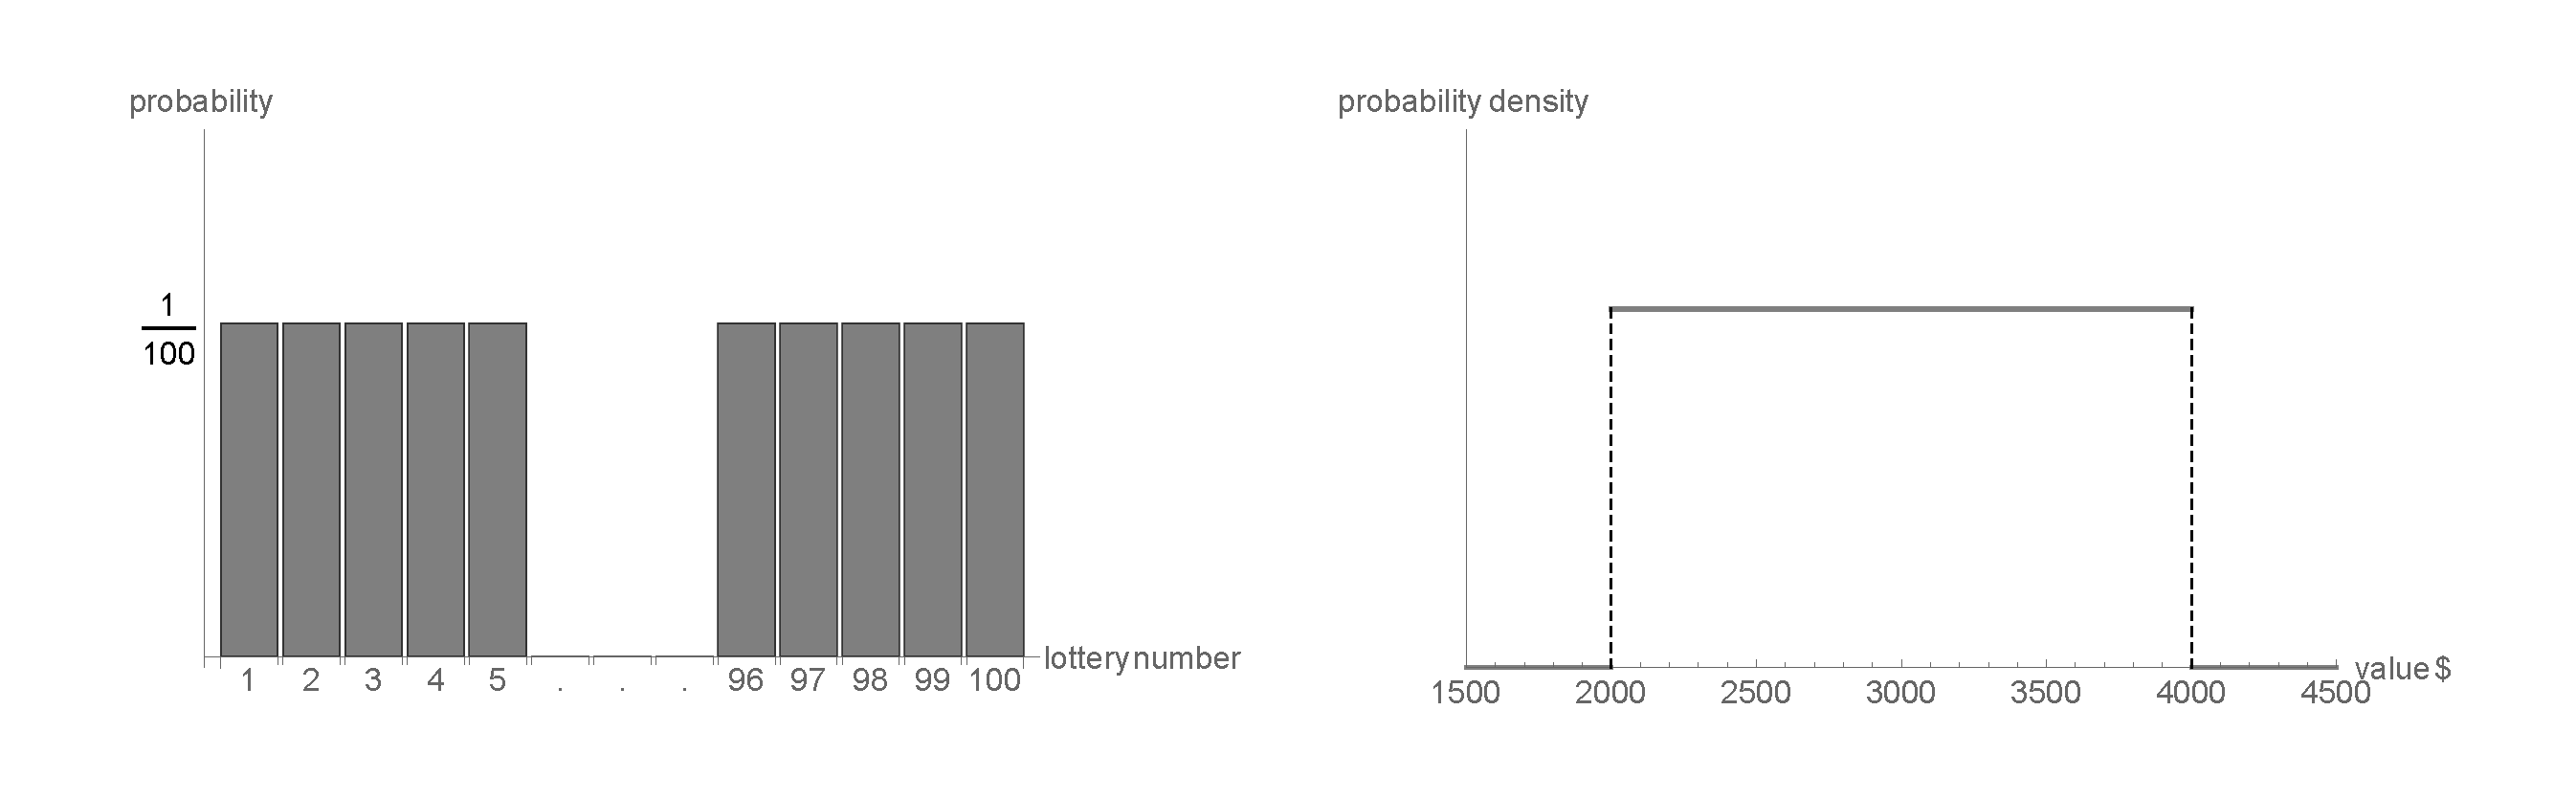
\includegraphics{Probability_lotterySecondhandCarProbability.pdf}}
\caption{Probability distributions representing \textbf{left:} the chance of winning a lottery, and \textbf{right:} the value of a second-hand car.}\label{fig:Probability_lotterySecondhandCarProbability}
\end{figure}

\subsection{What make a probability distribution \textit{valid}?}\label{sec:Probability_validProbabilityDistribution}
The lottery example given in section \ref{sec:Probability_probabilityDistributions} refers to discrete probability distribution, since the variable we were measuring - the winning number - is confined to take on finite set of values. However, we could similarly define a probability distribution where our variable is able to take on an infinity of values across a spectrum. Imagine that before test drive a second-hand car we are uncertain about its value. We might think that from seeing pictures of the car, that it could be worth anywhere from \$2000 to \$4000, with all values being equally likely (see \ref{fig:Probability_lotterySecondhandCarProbability}).

The aforementioned examples are both examples of valid/proper probability distributions. So, what are their defining properties?

\begin{itemize}
\item All values of the distribution must be real, and non-negative.
\item The sum (integral) across all possible values of the discrete (continuous) random variable must be 1.
\end{itemize}

In the lottery case, this is satisfied since $p(X)=\frac{1}{100}\geq 0$, and:

\begin{equation}
\frac{1}{100} + \frac{1}{100} + ... + \frac{1}{100} = \sum\limits_{i=1}^{100} \frac{1}{100} = 1
\end{equation}

For the continuous case of the probability of a heads when flipping a coin, the probability distribution is always $\frac{1}{2000}\geq 0$, and when we do the continuous analogue of summing - integrating - we find that:

\begin{equation}
\begin{align}
\int\limits_{2000}^{4000} p(v) \mathrm{d}v &= \int\limits_{2000}^{4000} \frac{1}{2000} \mathrm{d}v\\
&= \left[\frac{1}{2000}v\right]^{4000}_{2000}\\
&= \frac{1}{2000}\left(4000-2000\right)\\
&= 1
\end{align}
\end{equation}

Although, it may seem that this definition is relatively arbitrary, and perhaps well-trodden-territory for some readers, it is of \textit{central} importance to Bayesian statistics. This is because Bayesians like to work with, and produce \textit{valid} probability distributions. The pursuit of this ideal underlies the majority of \textit{all} methods in applied Bayesian statistics - analytic and computational - and hence its importance cannot be overstated!

\subsection{Probabilities vs probability density : interpreting discrete and continuous probability distributions}\label{sec:Probability_densityVsMassFunctions}
The discrete probability distribution for the lottery shown on the left hand side in figure \ref{fig:Probability_lotterySecondhandCarProbability}, is straightforward to interpret. To calculate the probability that the winning number, $X$, is 3, we simply read off the probability from the graph corresponding to the height of the leftmost bar, and find that:

\begin{equation}
p(X=3)= \frac{1}{100}
\end{equation}

In the discrete case, if we want to calculate the probability that a random variable takes on a range of values, then we simply need to sum the individual probabilities corresponding to each specific event. In the die example, if we want to calculate the probability that the winning number is 10 or less, we just add together the probabilities of it being \{1, 2, 3, 4, 5, 6, 7, 8, 9, 10\}:

\begin{equation}
\begin{align}
p(X\leq 10) &= p(X=1) + p(X=2) + p(X=3) + ... + p(X=9) + p(X=10)\\
&= \frac{1}{100} + \frac{1}{100} + \frac{1}{100} + ... + \frac{1}{100} + \frac{1}{100}\\
&= \frac{1}{10}
\end{align}
\end{equation}

How can we use the continuous probability distribution such as the one shown on the right hand side of figure \ref{fig:Probability_lotterySecondhandCarProbability}? If we want to calculate the probability that the value of the second-hand car is \$2,500, then we could simply draw a vertical line from this point on the $value$ axis up to the line of the distribution; concluding that $p(value=\$2,500) = \frac{1}{2000}$! However, under this logic, we could also deduce that the probability of the value of the car being \{\$2,500,\$2,500.10,\$2,500.01,\$2,500.001\} are all $\frac{1}{2000}$. Furthermore, we could generate an infinity of these test values of $value$, meaning that if we summed them all together we could get a total probability of $\infty$. 

There is evidently something wrong with our method for interpreting continuous densities. If we reconsider the test values $\{\$2,500,\$2,500.10,\$2,500.01,\$2,500.001\}$, we reason that these are all equally unlikely, and part of a set of an infinity of potential values we could draw. This means for a continuous random variable, we always have $p(\theta=number) = 0$. Hence, when we write $p(\theta)$ for a continuous random variable, we should be careful to interpret the value of it at a particular value as a probability \textit{density}, \textit{not} a probability. 

However, we can use a continuous probability distribution to calculate the probability that a random variable lies between two bounds. To do this we use the continuous analogue of a sum, an \textit{integral}. For the car example, we can calculate, $\$2,500\leq \theta \leq \$3,000$:

\begin{equation}\label{eq:Probability_continuousProbabilityIntervalExample}
\begin{align}
Pr(2500\leq value \leq 3000) &= \int\limits_{2500}^{3000} p(v) \mathrm{d}v\\
&= \int\limits_{2500}^{3000} \frac{1}{2000} \mathrm{d}v\\
&= \left[\frac{1}{2000}v\right]_{2500}^{3000}\\ 
&= \frac{1}{2000}(3000-2500) = 0.25
\end{align}
\end{equation}

In (\ref{eq:Probability_continuousProbabilityIntervalExample}), we have used $Pr$ to explicitly state that the result is a \textit{probability}, whereas $p(\theta)$ is a probability density. Of course, the calculation carried out in (\ref{eq:Probability_continuousProbabilityIntervalExample}), is equivalent to working out the area under the graph within those limits (see figure \ref{fig:Probability_continuousLotteryInterval}).

\begin{figure}
\centering
\scalebox{0.5} 
{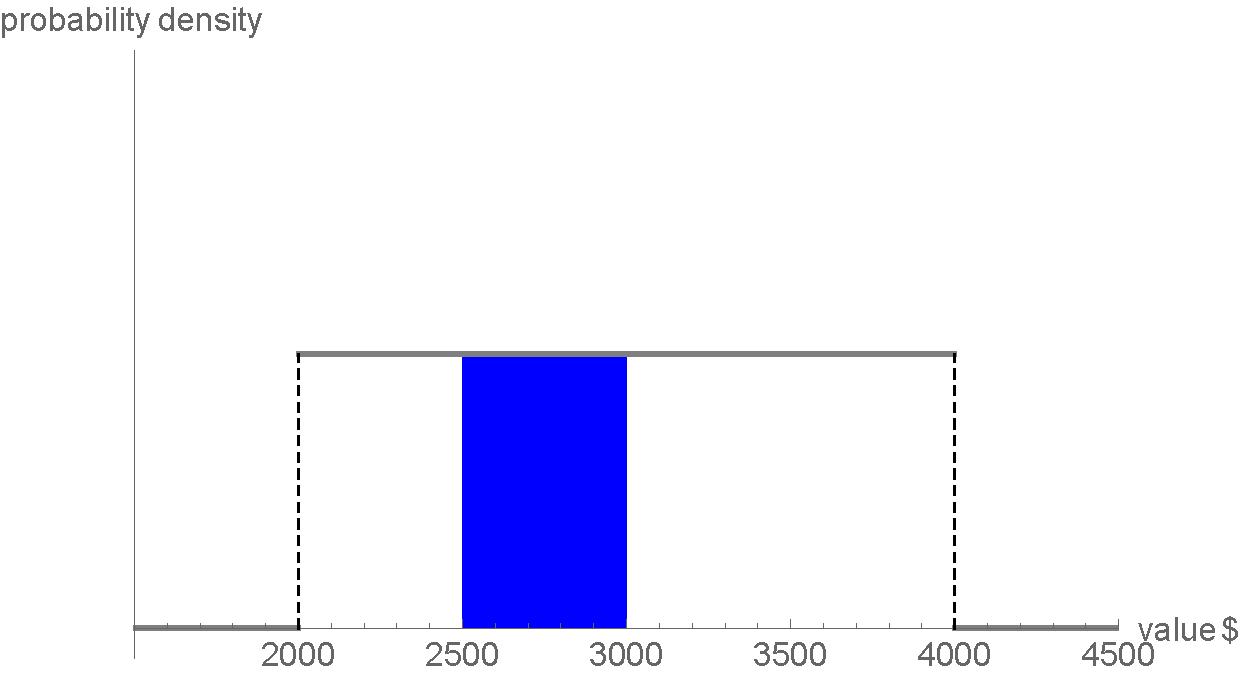
\includegraphics{Probability_continuousLotteryInterval.pdf}}
\caption{The probability that a second-hand car's value lies between \$2,500 and \$3,000.}\label{fig:Probability_continuousLotteryInterval}
\end{figure}

\boxed{Interactive:} see the interactive tool to allow you to dynamically manipulate figure \ref{fig:Probability_continuousLotteryInterval}.

\subsubsection{Analogy: stepping stones vs containers}
Imagine you wish to cross a fast-flowing river to reach friends on the other side. Fortunately, a helpful person has laid out stepping stones across the river's width. Wanting to demonstrate his mathematical skill, he has made the height of each stone, part of a valid probability distribution. In this discrete environment, the height of each stone exactly determines the probability (see figure \ref{fig:Probability_steppingStones}). 

By contrast, imagine a filled container of water. The mass of the entire container is set to equal 1. If you were to calculate the probability that a single water molecule lies within a given volume of the container, all we need to do is calculate the mass of that element. We do this by first calculating the element's volume, then multiplying through by the density (in this example, the density is constant). Note here, we can't use probability density directly; we need to calculate a corresponding volume in order to get a probability.

\begin{figure}
\centering
\scalebox{0.6} 
{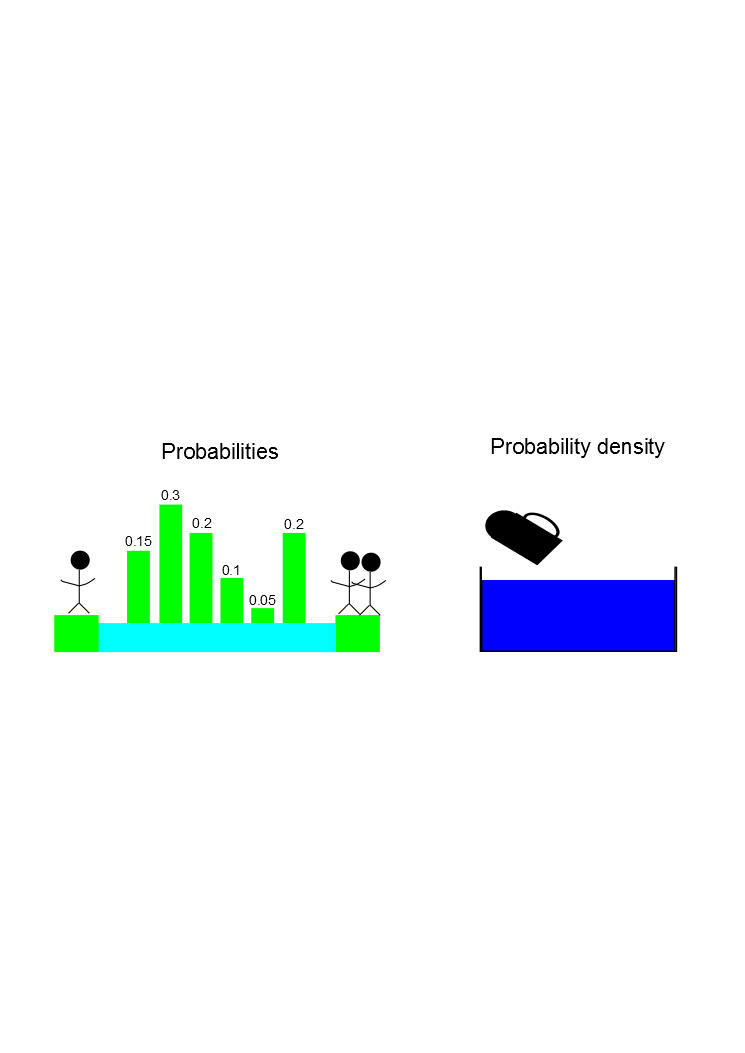
\includegraphics{Probability_steppingStones.png}}
\caption{Left: a discrete probability distribution, and corresponding probabilities. Right: a probability density.}\label{fig:Probability_steppingStones}
\end{figure}

A quick note on terminology: often theorists use probability \textit{mass} to handle discrete distributions, where the distribution's values are directly interpretable as probabilities, and probability \textit{densities} to handle continuous distributions. The latter need to be integrated to yield a probability. We eschew the 'mass' terminology as we find it counter-productive to differentiate between the two types of distributions, since Bayes' rule handles them in the same way (see below).

\boxed{Video:} see the video XXX which explains more about the difference between a probability and a probability density.

\subsubsection{The good news: Bayes' rule doesn't distinguish between probabilities and probability densities}
Whilst it is important to understand that probabilities and probability densities are \textit{not} the same type of entity, the good news for us is that Bayes' rule is the same for each. So we can readily write:

\begin{equation}
Pr(\theta=1|X=1) = \frac{Pr(X=1|\theta=1)Pr(\theta=1)}{Pr(X=1)}
\end{equation}

for the case of when the data, $X$, and the parameter $\theta$ are discrete, and hence $Pr$ denotes a probability.

Alternatively, we can write Bayes' rule as:

\begin{equation}
p(\theta=1|X=1) = \frac{p(X=1|\theta=1)p(\theta=1)}{p(X=1)}
\end{equation}

for the case when the data and parameter are continuous, and $p$ denotes a probability density.

We will more commonly use the latter representation since for the majority of cases, the parameters will be continuous.

\subsection{Mean and variance of distributions}\label{sec:Probability_meanVariance}
A popular way of summarising a distribution is via its \textit{mean}, which is one measure of central tendency of a distribution. More intuitively, a mean, or \textit{expected value}, of a distribution represents the long-run average value that would be obtained if we sampled from that particular distribution in question, an infinite number of times. 

The way in which we calculate the \textit{mean} of a distribution depends on whether it is \textit{discrete} or \textit{continuous} in nature. However, the concept is essentially the same in both cases. The mean is calculated as a weighted sum of the values taken on by the random variable in question, where the weights are provided by the probability distribution. This results in the following forms for the mean of a discrete and continuous variable respectively:

\begin{equation}\label{eq:Probability_meanDistributionDiscrete}
\mathbb{E}(X) = \sum\limits_{All\; \alpha} \alpha Pr(X=\alpha)
\end{equation}

\begin{equation}\label{eq:Probability_meanDistributionContinuous}
\mathbb{E}(X) = \int\limits_{All\; \alpha} \alpha p(\alpha)\mathrm{d}\alpha
\end{equation}

In (\ref{eq:Probability_meanDistributionDiscrete}) and (\ref{eq:Probability_meanDistributionContinuous}), $\alpha$ represents the multitude, or continuum of \textit{values} taken on by the random variable $X$ respectively.  We have chosen to use $Pr$ in (\ref{eq:Probability_meanDistributionDiscrete}), and $p$ in (\ref{eq:Probability_meanDistributionContinuous}), to illustrate that these represent probabilities and probability \textit{densities} respectively.

We can now apply (\ref{eq:Probability_meanDistributionDiscrete}) to allow us to calculate the mean winning number from the lottery:

\begin{equation}\label{eq:Probability_meanLottery}
\begin{align}
\mathbb{E}(X) &= \sum\limits_{\alpha=1}^{100} \alpha Pr(X=\alpha)\\
&= 1\times\frac{1}{100} +  2\times\frac{1}{100} +  3\times\frac{1}{100} + ... +  99\times\frac{1}{100} +  100\times\frac{1}{100}\\
&= 50\tfrac{1}{2}
\end{align}
\end{equation}

We can also demonstrate the \textit{long-run} nature of the mean value of $50\tfrac{1}{2}$ found in (\ref{eq:Probability_meanLottery}) by simulating a number of rolls of a fair die computationally (see figure \ref{fig:Probability_meanDiscreteLongRun}). As the number of rolls increases, the running mean tends towards this value.

\begin{figure}
\centering
\scalebox{0.55} 
{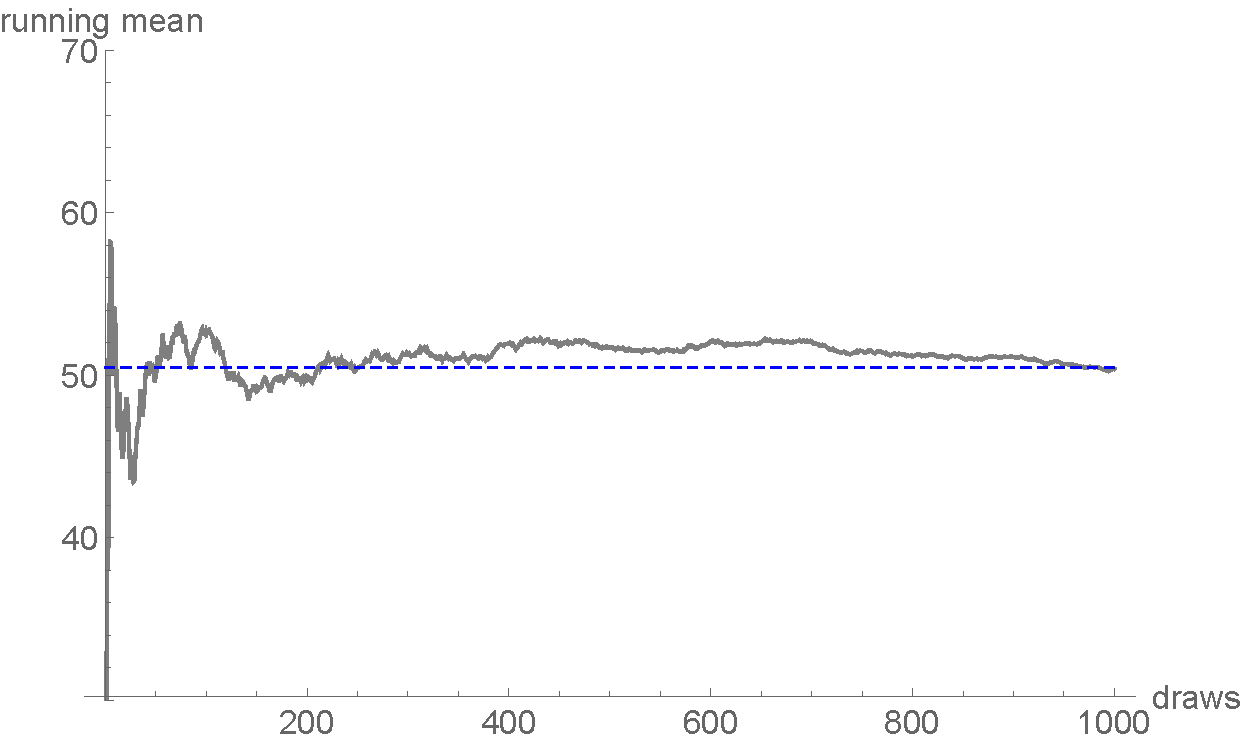
\includegraphics{Probability_meanDiscreteLongRun.pdf}}
\caption{Playing a computational lottery. We see the approach of the running mean of repeatedly playing the lottery to the long-run mean of $50\tfrac{1}{2}$, as the number of plays increases.}\label{fig:Probability_meanDiscreteLongRun}
\end{figure}

We can also apply (\ref{eq:Probability_meanDistributionContinuous}) to calculate our expectation of the second-hand car value:

\begin{equation}\label{eq:Probability_meanCoinContinuous}
\begin{align}
\mathbb{E}(value) &= \int\limits_{2000}^{4000} v p(v)\mathrm{d}v\\
&=\frac{1}{2000} \int\limits_{2000}^{4000} v \mathrm{d}v\\
&= \frac{1}{2000}\left[\frac{v^2}{2}\right]^{4000}_{2000}\\ 
&= \$3,000
\end{align}
\end{equation}

If we were to have a business buying (and selling) second-hand cars, we might keep tabs on the values of cars we buy over time. If all cars came from the same uniform distribution that we have proposed, then we would see the sample average value approaching the above long-run mean of \$3,000, as the number of cars we buy gets large\footnote{Technically, tends to infinity.} (see figure \ref{fig:Probability_meanContinuousLongRun}).

\begin{figure}
\centering
\scalebox{0.55} 
{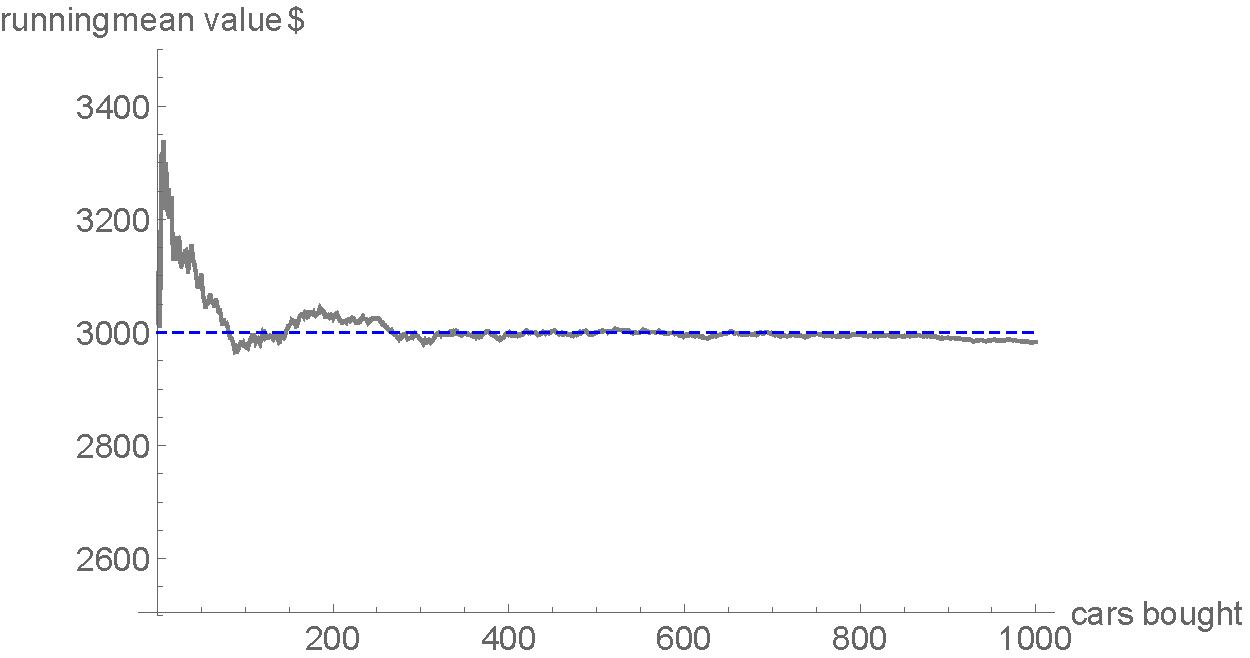
\includegraphics{Probability_meanContinuousLongRun.pdf}}
\caption{Career second-hand car sales. We can see the approach of the sample mean towards the long-run mean of \$3,500.}\label{fig:Probability_meanContinuousLongRun}
\end{figure}

If you can grasp the process undertaken to produce figures \ref{fig:Probability_meanDiscreteLongRun} and \ref{fig:Probability_meanContinuousLongRun} respectively, then you already understand the basis behind modern computational Bayesian statistics! If you need a bit more explanation of the theory of Bayesian computational, then fear not, we devote an entire Part of the book for this purpose (see Part \ref{part:computationalBayes}).  

Whilst the \textit{mean} of a distribution is a measure of central tendency for a particular distribution, we do not yet have a way of summarising the width of the range of the values of the random variable which are most likely. This motivates the introduction of the concept of a \textit{variance} of a distribution:

\begin{equation}\label{eq:Probability_varianceDistributionExpectations}
var(X) = \mathbb{E}\left(\left[X-\mathbb{E}(X)\right]^2\right)
\end{equation}

To apply (\ref{eq:Probability_varianceDistributionExpectations}) to discrete and continuous distributions respectively, we straightforwardly replace the $\alpha$ on the right-hand side of (\ref{eq:Probability_meanDistributionDiscrete}) and (\ref{eq:Probability_meanDistributionContinuous}) respectively, by $(\alpha-\mathbb{E}(X))^2$ in each case\footnote{This is a specific example of the general rule, that to calculate the mean value of some function $f(X)$, where $X$ is governed by a particular distribution, we do: \begin{equation}
\mathbb{E}(f(X)) = \sum\limits_{All\; \alpha} f(\alpha) Pr(X=\alpha)
\end{equation}
for a discrete distribution, and analogously for the continuous case, but using an integral opposed to a sum.}:

\begin{equation}\label{eq:Probability_varianceDistributionDiscrete}
var(X) = \sum\limits_{All\; \alpha} (\alpha-\mathbb{E}(X))^2 Pr(X=\alpha)
\end{equation}

\begin{equation}\label{eq:Probability_varianceDistributionContinuous}
var(X) = \int\limits_{All\; \alpha} (\alpha-\mathbb{E}(X))^2 p(\alpha)\mathrm{d}\alpha
\end{equation}

If the equations are starting to overwhelm, then fret not, we really only wanted to include them for completeness. What is more important is their significance. Essentially, a \textit{variance} measures the width of the distribution of values obtained around its mean. A wider variance therefore signifies a greater variety of values away from the mean. In figure \ref{fig:Probability_varianceLottery} we compare the variability of the fair lottery, with one heavily biased to take on the values between 40 and 60. We see that the variability of the running mean for the biased lottery is smaller than that of the fair one, particularly as the number of rolls increases. This is due to the fact that the fair lottery has a variance of:

\begin{equation}
\begin{align}
var(X) &= \sum\limits_{\alpha=1}^{100} (\alpha-50\tfrac{1}{2})^2\times Pr(X=\alpha)\\
&= 833\tfrac{1}{4}
\end{align}
\end{equation}

whereas similar calculations for the loaded die distribution shown in the middle of figure \ref{fig:Probability_varianceLottery}, yield a value of approximately 265. To be concrete, the variance of a distribution is an indicator of the long-run average square distance of values away from the mean. 

\begin{figure}
\centering
\scalebox{0.35} 
{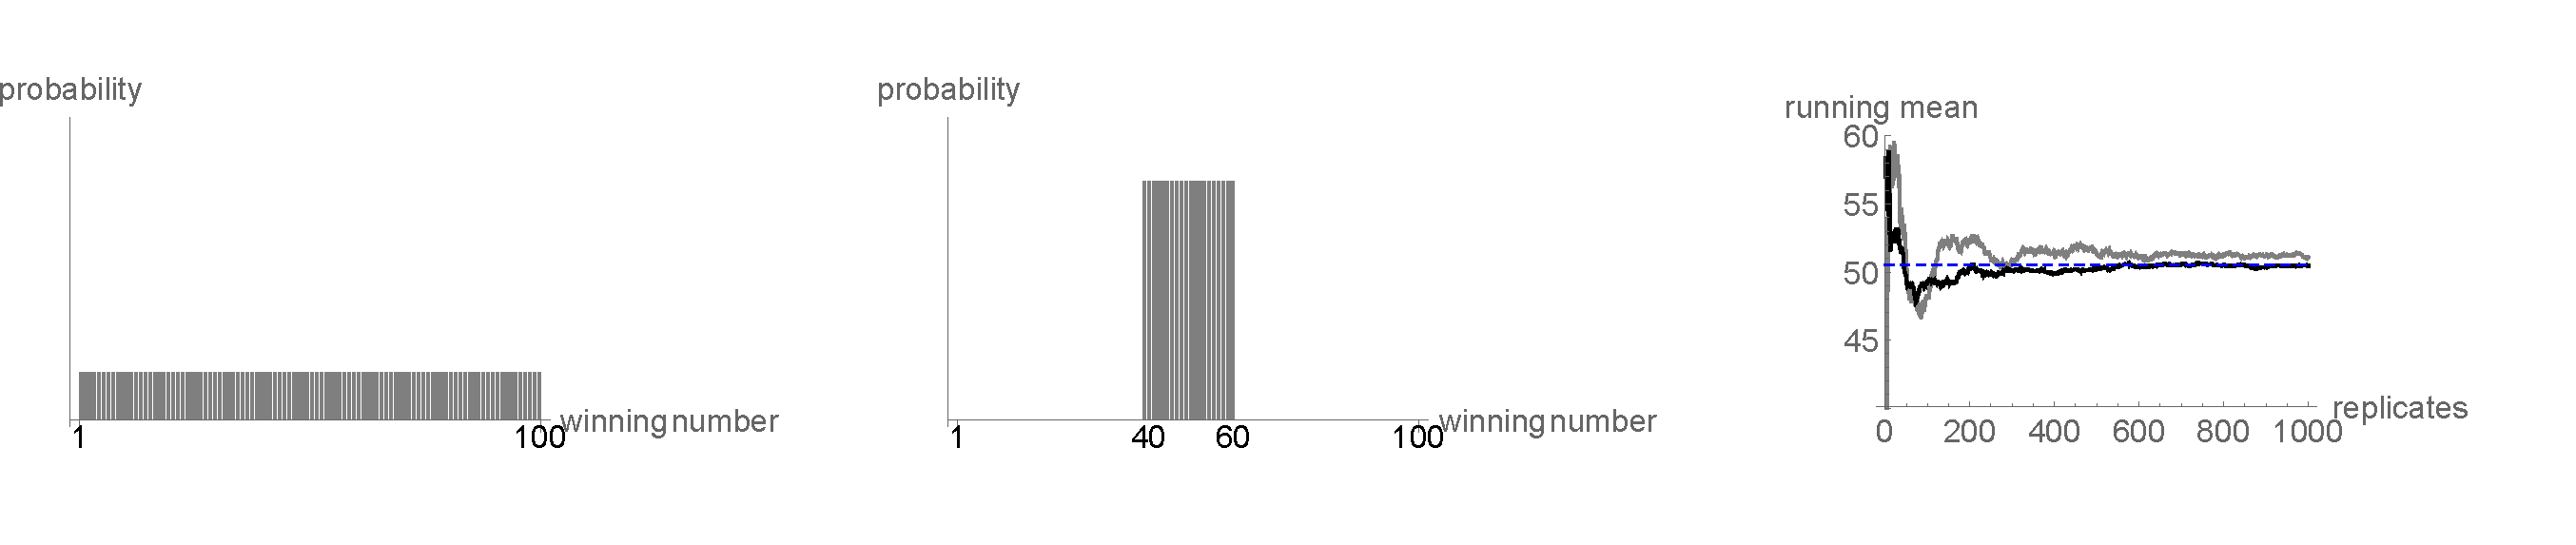
\includegraphics{Probability_varianceLottery.pdf}}
\caption{Comparing the variance of two lotteries, left: a lottery where all values between 0 and 100 are equally likely. Middle: a lottery where only values between 40 and 60 have a positive probability. Right: comparing the variability of these distributions about their common mean.}\label{fig:Probability_varianceLottery}
\end{figure} 

\subsection{Generalising probability distributions to two dimensions}
Life is often more complex than the examples of section \ref{sec:Probability_probabilityDistributions}. Often we are tasked with formulating opinions on a range of different outcomes; each of which may influence or shed light on the other results. We begin by considering the outcome of two measurements, in order to introduce the reader to the mechanics of probability. The great thing is that these rules do not become any more complex when we generalise to higher dimensional problems, meaning that if the reader is comfortable with the following examples, then they should be able to handle the vast majority of probability distribution operations encountered. In Bayesian statistics, being comfortable manipulating probability distributions is essential, since the output of the Bayesian formula - the posterior probability distribution - is used to derive all post-experiment conclusions. As such, it is important to devote some time to introduce two examples which we will use to describe and explain the manipulations of 2-dimensional probability distributions.

\subsubsection{Horses for courses: a 2-dimensional discrete probability example}\label{sec:Probability_biasedCoinsTwoDimensionalDiscrete}
Imagine that you are a horse racing aficionado, and are interested in quantifying the uncertainty regarding the outcome of two (fictitious) races for two thoroughbreds in a particular stable. From their historical performance over 100 races you notice that both horses tend to react in the same way to the racing conditions. When horse A wins, it is more likely that, later in the day, horse B will win, and vice versa. Similarly regarding the losses; when horse A finds the going tough, so does horse B. Wanting to flex your statistical muscle, you choose to represent this information by the two-dimensional probability distribution shown in table \ref{tab:Probability_coinBiased}

\begin{table}[htbp]
  \centering
    \begin{tabular}{rrcc}
    \toprule
          &       & \multicolumn{2}{c}{\textbf{horse A}} \\
    \midrule
          &       & \textbf{0} & \textbf{1} \\
    \multicolumn{1}{c}{\textbf{horse B}} & \multicolumn{1}{c}{\textbf{0}} & $\frac{30}{100}$   & $\frac{10}{100}$ \\
    \multicolumn{1}{c}{} & \multicolumn{1}{c}{\textbf{1}} & $\frac{10}{100}$   & $\frac{50}{100}$ \\
    \bottomrule
    \end{tabular}%
  \caption{A probability distribution showing the historical performance of two horses, A and B, in two separate races. $\{0,1\}$ refers to each horse losing or winning in their respective races.}\label{tab:Probability_coinBiased}
\end{table}

How can we check whether this distribution satisfies the requirements for a valid probability distribution? We simply apply the rules described in section \ref{sec:Probability_validProbabilityDistribution}. Firstly, all the values of the distribution are real and non-negative; satisfying our first requirement. For the second rule rather than summing over the values of one random variable, we now have to sum over the outcome of two:

\begin{equation}\label{eq:Probability_discreteTwoDimensionalCoinSum}
\sum\limits_{X_A=0}^{1}\sum\limits_{X_B=0}^{1} Pr(X_A,X_B) = \frac{30}{100} + \frac{10}{100}  + \frac{10}{100}  + \frac{50}{100}  = 1
\end{equation}

In (\ref{eq:Probability_discreteTwoDimensionalCoinSum}), $X_A$ and $X_B$ are random variables\footnote{A function which associates a unique numerical value with each outcome of an experiment. In this case the function gives value 0 if the result is a tails, and 1 if it is heads.} which refer to the outcome of the races for horse A and horse B respectively. Notice that since we are now considering a situation with the outcome of two random variables, we are now required to index the probability, $Pr(X_A,X_B)$, by both. Due to the probability now being a function of two variables, we say that the probability distribution is 2-dimensional.

How can we interpret the probability distribution shown in table \ref{tab:Probability_coinBiased}? The probability that both horses lose (and hence both their random variables take on the value of 0), is simply read off from the top-left entry in the table, meaning $Pr(X_A=0,X_B=0)=\frac{30}{100}$. We ascribe a smaller likelihood to heterogeneous outcomes, $Pr(X_A=0,X_B=1)=\frac{10}{100}$ or $Pr(X_A=1,X_B=0)=\frac{10}{100}$, since we believe that the horses are more likely to react similarly to the racing conditions. We believe that the most likely outcome is that both horses win, since historically the horses have done well on this particular racing course, and hence ascribe the highest probability to this result, with $Pr(X_A,X_B)=\frac{50}{100}$.

\subsubsection{Foot length and literacy: a 2-dimensional continuous probability example}
We suppose that we have a sample of individuals, and we measure their foot size, as well as how well they score on a literacy test. Both of these variables can reasonably be assumed to be continuous, meaning that we are now required to represent our strength of belief, by specifying a probability distribution across a continuum of values (see figure \ref{fig:Probability_footSizeIntelligenceTwoDimensionalExample}). 

\begin{figure}
\centering
\scalebox{0.5} 
{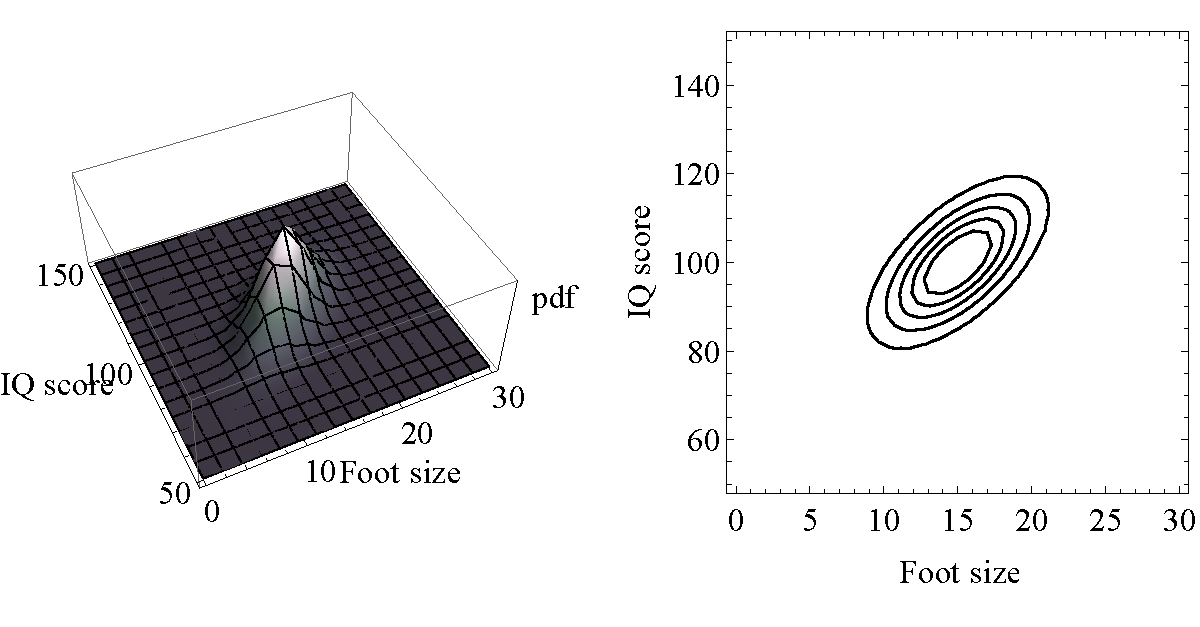
\includegraphics{Probability_footSizeIntelligenceTwoDimensionalExample.pdf}}
\caption{A probability distribution describing the foot size and scores on a literacy test for an individual within our sample. Left) Represented as a 3-dimensional plot, and Right) Contour lines specify isolines of probability.}\label{fig:Probability_footSizeIntelligenceTwoDimensionalExample}
\end{figure}

We could verify that the distribution shown in figure \ref{fig:Probability_footSizeIntelligenceTwoDimensionalExample} is in fact valid, by showing that the volume underneath the left hand plot is 1, via integration. However, since we don't want to overcomplicate things now, you will have to take our word for it.

Notice that there to be a degree of correlation between foot size and scores on the literacy test. Why might this be the case\footnote{Our sample of individuals here is a sample of children of various ages. Age is correlated with shoe size and literacy.}?

\subsection{Marginal distributions}\label{sec:Probability_marginal}
We may be interested in simplifying the preceding analysis, by stating the distribution of one variable, completely \textit{unconditional} of the other. In our horses example, we might be interested in say, only the result of the first horse race, which involves horse A. Alternatively, we might want to remove the dependence on foot size, in our literacy score example, and what remains would then be an \textit{unconditional} probability distribution for literacy score.

In order to do this, we essentially need to \textit{average} out the dependence of the other variable. In our horses example, if we are only interested in the result of horse A, we can sum down the column values for horse B, obtaining the \textit{marginal} distribution of horse A, shown at the bottom of table \ref{tab:Probability_coinsMarginal}.


\begin{table}[htbp]
  \centering
    \begin{tabular}{rrccr}
    \toprule
          &       & \multicolumn{2}{c}{\textbf{horse A}} &  \\
    \midrule
          &       & \textbf{0} & \textbf{1} & \multicolumn{1}{c}{\textbf{$Pr(X_B)$}} \\
    \multicolumn{1}{c}{\textbf{horse B}} & \multicolumn{1}{c}{\textbf{0}} & $\frac{30}{100}$   & $\frac{10}{100}$    & \multicolumn{1}{c}{\textbf{$\frac{40}{100}$ }} \\
    \multicolumn{1}{c}{} & \multicolumn{1}{c}{\textbf{1}} & $\frac{10}{100}$    & $\frac{50}{100}$    & \multicolumn{1}{c}{\textbf{$\frac{60}{100}$ }} \\
          & \multicolumn{1}{c}{\textbf{$Pr(X_A)$}} & \textbf{$\frac{40}{100}$ } & \textbf{$\frac{60}{100}$ } & \multicolumn{1}{c}{} \\
    \bottomrule
    \end{tabular}%
  \caption{The marginal distribution of horses A and B, achieved by summing the values in each column or row respectively.}\label{tab:Probability_coinsMarginal}%
\end{table}%

Hence, we have that the \textit{marginal} probability of horse A winning is 0.6. This value is composed out of the two possible ways in which this \textit{single} event can occur:

\begin{equation}\label{eq:Probability_marginalCoinsExample}
Pr(X_A=1) = Pr(X_A=1,X_B=0) + Pr(X_A=1,X_B=1)
\end{equation}

In (\ref{eq:Probability_marginalCoinsExample}), we see that A can win with B losing, or alternatively both horses can win.

Thus, in order to calculate the probability of a single event, we simply need to sum across all possible occurrences of it, allowing the other variable to take on its possible values. Mathematically, we can summarise this rule by the following for the case of two discrete random variables:

\begin{equation}\label{eq:Probability_marginalDiscreteProbabilityTwoDimensions}
Pr(A=\alpha) = \sum\limits_{\beta} Pr(A=\alpha,B=\beta)
\end{equation}

In (\ref{eq:Probability_marginalDiscreteProbabilityTwoDimensions}), $\alpha$ and $\beta$ refer to the specific values taken on by the random variables $A$ and $B$. 

We can use (\ref{eq:Probability_marginalDiscreteProbabilityTwoDimensions}) for the horses example to calculate the probability that horse B loses:

\begin{equation}
\begin{align}
Pr(X_B=0) &= \sum\limits_{\alpha=0}^{1} Pr(X_B=0,X_A=\alpha)\\
&= Pr(X_B=0,X_A=0) + Pr(X_B=0,X_A=1)\\
&= \frac{30}{100}  + \frac{10}{100}  = \frac{40}{100} 
\end{align}
\end{equation}

For continuous random variables we need the continuous analogue of a sum, an \textit{integral}, in order to calculate the marginal distribution. Intuitively, this is because the other variable is now able to take on an continuum of values:

\begin{equation}\label{eq:Probability_marginalContinuousProbabilityTwoDimensions}
p_A(\alpha) = \int\limits_{All\;\beta} p_{AB}(\alpha,\beta) \mathrm{d}\beta
\end{equation}

In (\ref{eq:Probability_marginalContinuousProbabilityTwoDimensions}), $p_{AB}(\alpha,\beta)$ corresponds to the joint probability distribution of random variables $A$ and $B$ evaluated at $(A=\alpha,B=\beta)$. Similarly, $p_A(\alpha)$ refers to the marginal distribution of random variable A, evaluated at $A=\alpha$. Although it is somewhat of an abuse of notation, for simplicity, from now on we will now write $p_{AB}(\alpha,\beta)$ as $p(A,B)$, and $p_A(\alpha)$ as $p(A)$.

In the foot size/literacy example, we may not be interested in foot size; wanting only the distribution of literacy scores in our sample. We can obtain this by simply integrating out the dependence on foot size:

\begin{equation}\label{eq:Probability_marginalContinuousProbabilityTwoDimensionsFootExample}
p(score) = \int\limits_{0}^{30} p(score,FS) \mathrm{d}FS
\end{equation}

The result of carrying out the step in (\ref{eq:Probability_marginalContinuousProbabilityTwoDimensionsFootExample}) is that we are left with the distribution shown on the right of figure \ref{fig:Probability_footSizeIntelligenceMarginal}. We have rotated this graph to emphasise that it is the result of essentially summing\footnote{We really mean integrating, but it is more intuitive to think about this in terms of discrete summing.} across the joint density at each particular value of literacy scores. 

Another way to think about marginal densities, is imagine that you are walking along the landscape of the joint density. The total distance walked - horizontally and vertically - from $FS=0$ to $FS=30$ along a line of constant literacy, gives the height of the marginal density for literacy score at that point. If the path is relatively flat, indicating a low value of joint density, then the corresponding marginal density is low. However, if the path encompasses a large hill, indicating a high value of joint density, then the marginal density will be relatively high.

Add a 3D version of the figure with the contours traced out on the landscape, and leading to the height of the marginals, perhaps with stick figures walking along lines of iso-literacy.

\begin{figure}
\centering
\scalebox{0.5} 
{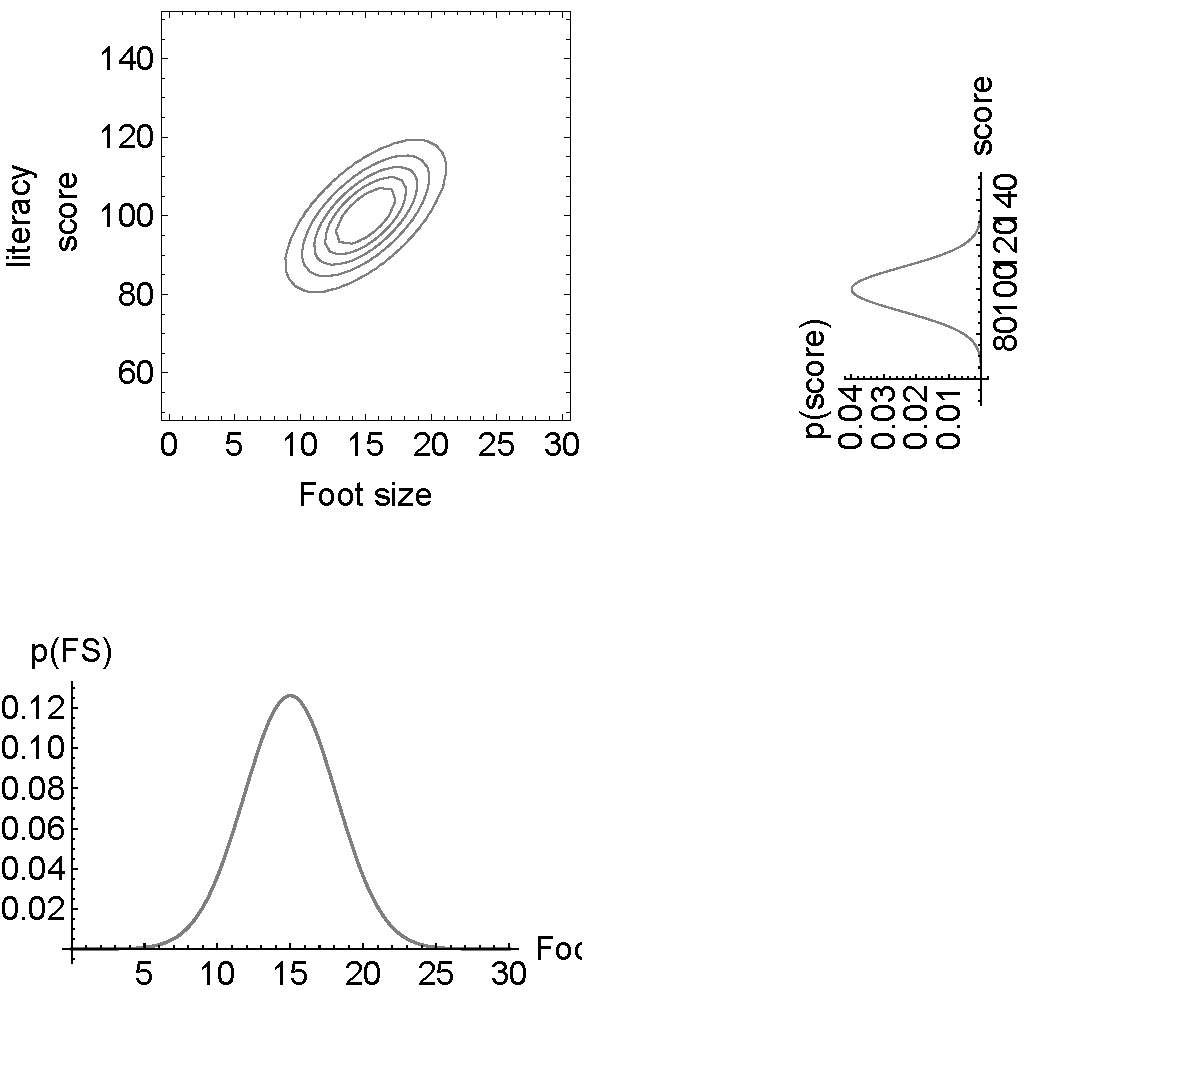
\includegraphics{Probability_footSizeIntelligenceMarginal.pdf}}
\caption{Top-left: the joint density of foot size and intelligence. Right: the marginal density of literacy scores. Bottom: the marginal density of foot size. \textbf{I want to add a line at a particular value of literacy scores, and at a particular value of FS, to illustrate the horizontal and vertical summing.}}\label{fig:Probability_footSizeIntelligenceMarginal}
\end{figure}

\subsubsection{Venn diagrams}
An alternative way of thinking about marginal distributions is provided by the Venn diagram shown in figure \ref{fig:Probability_Venn}. In a Venn diagram, the area of a particular event indicates its probability, and the rectangular area represents all the events that can possibly happen, and so has an area of 1. We have chosen to specify the events of horse A winning, and B winning A as sub-areas the diagram, which overlap indicating a region of joint probability, $p(X_A=1,X_B=1)$. In this set-up it is straightforward to calculate the marginal probability of horse A winning, or horse B; we find the area of the elliptic shapes A or B respectively. Considering horse A, when we calculate the area of the entire ellipse, we are implicitly carrying out the sum of the form indicated in (\ref{eq:Probability_marginalDiscreteProbabilityTwoDimensions}):

\begin{equation}\label{eq:Probability_vennMarginals}
p(A) = p(A,B) + p(A,not\; B)
\end{equation}

and are working out the probability that A wins unconditionally\footnote{Irrespective of what happens to B.}.

In (\ref{eq:Probability_vennMarginals}), the terms on the right hand side correspond to the overlap region, and the remaining part of A (where B does not occur) respectively.

\begin{figure}
\centering
\scalebox{0.5} 
{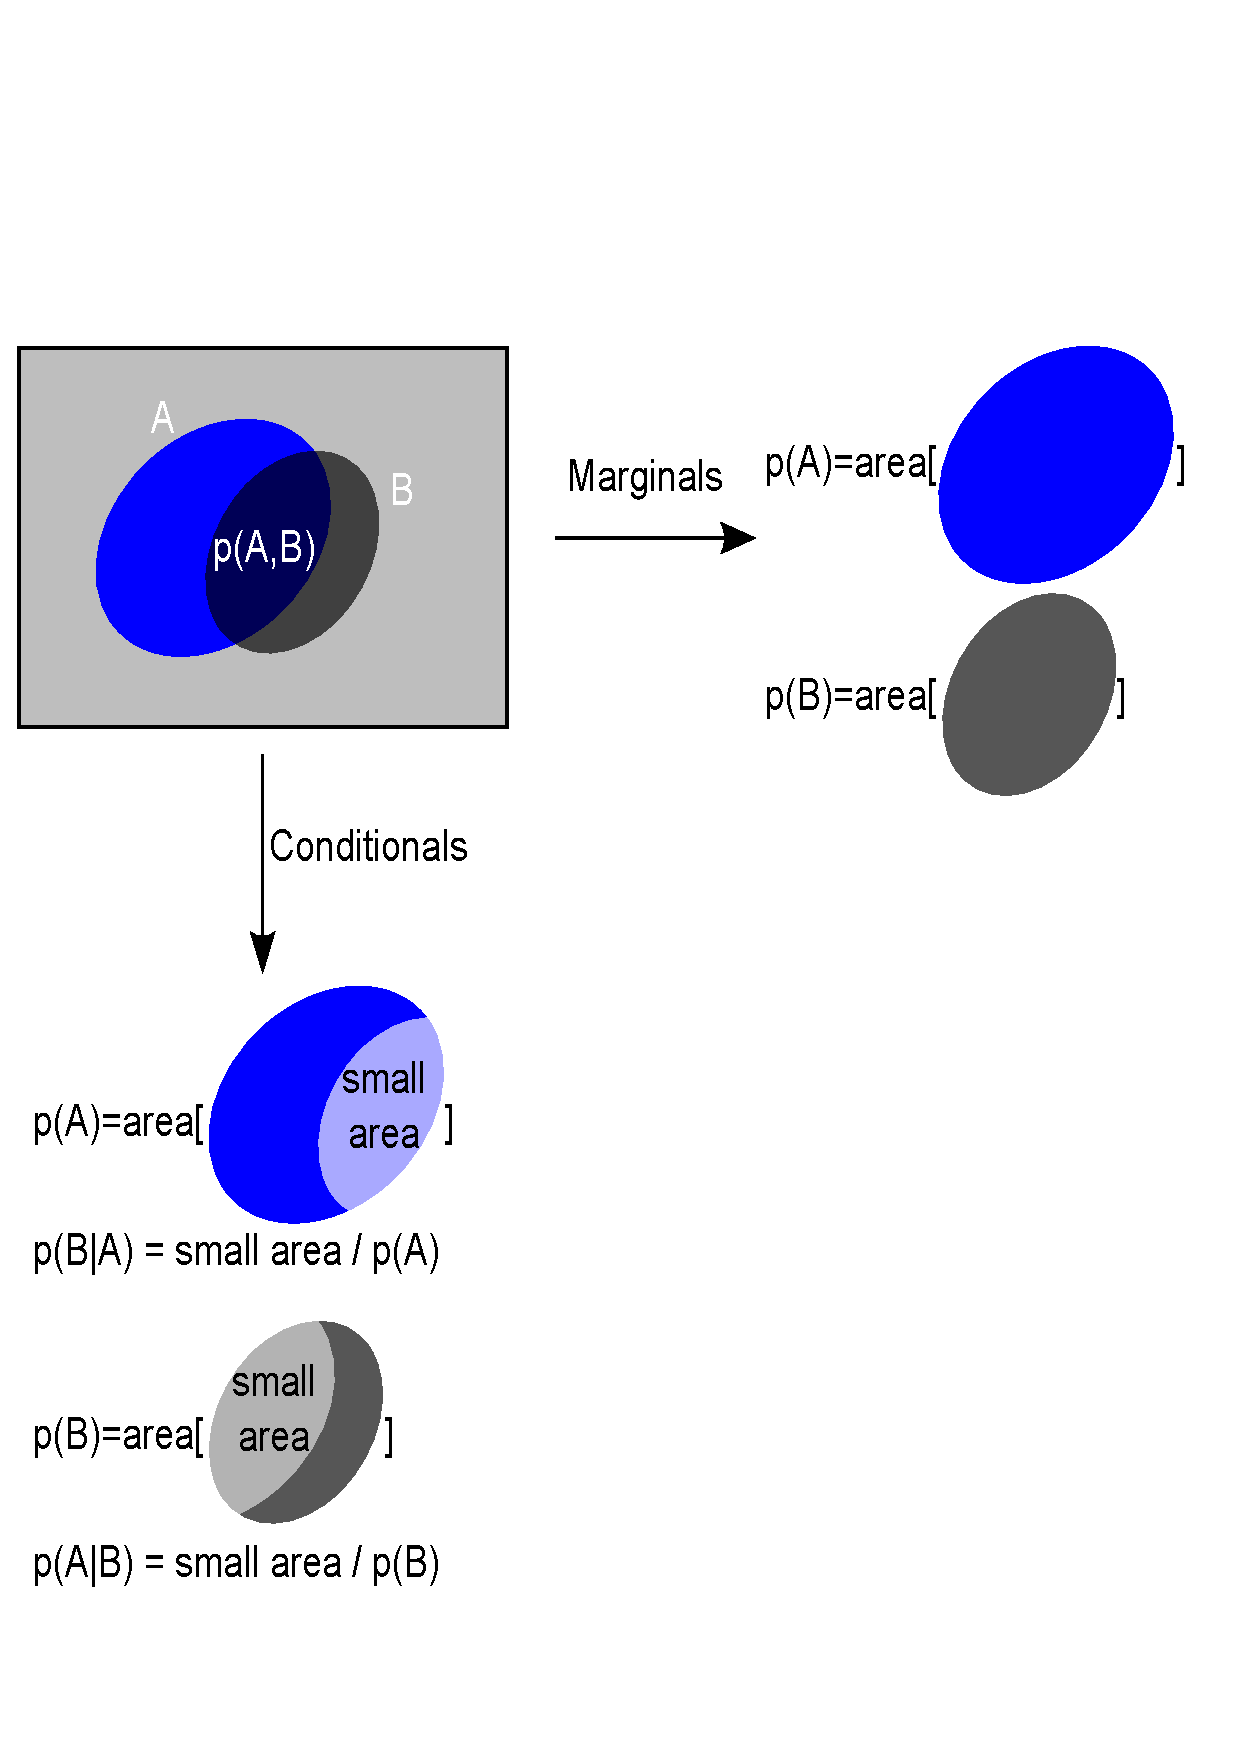
\includegraphics{Probability_Venn.pdf}}
\caption{A Venn diagram showing one way of interpreting marginal and conditional distributions for the horse racing example.}\label{fig:Probability_Venn}
\end{figure}

\subsection{Conditional distributions}\label{sec:Probability_conditionalDistributionIntro}
We sometimes only receive partial information by observing part of the system in which we are interested. In horses example, we might only see the result of one horse race, and on this basis update our probabilities of the other horse winning. Alternatively, in the foot size - literacy example described before, we might measure an individual's shoe size, and then want to obtain the updated probability distribution for literacy scores.

In probability, when we observe one variable, and reformulate the probability distribution for the other variable, we say that we are deriving the \textit{conditional} distribution of the latter. \textit{Conditional} refers to the fact that we are deriving the probability distribution of one variable, \textit{conditional} on the value of the other(s).

In each case, we have reduced some of the uncertainty in the system, by observing one of its characteristics. Hence in the two-dimensional examples described above the conditional distribution is only one-dimensional, because we are only now uncertain about one variable. 

Luckily, there is a simple rule that we can use to obtain the probability of one variable, conditional on the value of the other:

\begin{equation}\label{eq:Probability_conditionalProbability}
p(A|B) = \frac{p(A,B)}{p(B)}
\end{equation}

In (\ref{eq:Probability_conditionalProbability}), $p(A|B)$ refers to the probability of $A$ occurring, given that $B$ has occurred. In the right hand side of (\ref{eq:Probability_conditionalProbability}), $p(B)$ is the \textit{marginal} distribution of B occurring, and $p(A,B)$ is the joint probability of $A$ and $B$ occurring.

We can use (\ref{eq:Probability_conditionalProbability}) for the horses example to calculate the probability that \textit{given} that horse A wins, what is the probability of horse B also winning?

\begin{equation}\label{eq:Probability_conditionalDiscreteCoins}
\begin{align}
Pr(X_B=1|X_A=1) &= \frac{Pr(X_A=1,X_B=1)}{Pr(X_A=1)}\\
&= \frac{Pr(X_A=1,X_B=1)}{Pr(X_A=1,X_B=0)+Pr(X_A=1,X_B=1)}\\
&= \frac{\frac{50}{100}}{\frac{10}{100} + \frac{50}{100}}\\ 
&= \frac{5}{6}
\end{align}
\end{equation}

In (\ref{eq:Probability_conditionalDiscreteCoins}), we have used the rule we discussed earlier for calculating marginal probabilities, shown in (\ref{eq:Probability_marginalDiscreteProbabilityTwoDimensions}), to calculate the denominator, $Pr(X_A=1)$ (allowing us to move from line 1 to 2).

Another way to see the workings of this calculation is shown in table \ref{tab:Probability_coinsConditionalDiscrete}. When we see that horse A wins, we essentially reduce our solution space to only the central column (highlighted in blue). Therefore we need to renormalise the solution space such that it has a probability of 1, by dividing each of its entries through by its original total of probabilities, 0.6; yielding the conditional probabilities shown in the right hand column of table \ref{tab:Probability_coinsConditionalDiscrete}.

\begin{table}[htbp]
  \centering
    \begin{tabular}{rrccr}
    \toprule
          &       & \multicolumn{2}{c}{\textbf{horse A}} &  \\
    \midrule
          &       & \textbf{0} & \textbf{1} & \multicolumn{1}{c}{\textbf{$Pr(X_B|X_A=1)$}} \\
    \multicolumn{1}{c}{\textbf{horse B}} & \multicolumn{1}{c}{\textbf{0}} & $\frac{30}{100}$   & {\color{blue}$\frac{10}{100}$ }   & \multicolumn{1}{c}{\textbf{=$\frac{10}{100}$ /$\frac{60}{100}$  = $\frac{1}{6}$ }} \\
    \multicolumn{1}{c}{} & \multicolumn{1}{c}{\textbf{1}} & $\frac{10}{100}$   & {\color{blue}$\frac{50}{100}$ }   & \multicolumn{1}{c}{\textbf{=$\frac{50}{100}$ /$\frac{60}{100}$  = $\frac{5}{6}$ }} \\
          & \multicolumn{1}{c}{\textbf{$Pr(X_A)$}} & \textbf{$\frac{40}{100}$ } & {\color{blue}\textbf{$\frac{60}{100}$ }} & \multicolumn{1}{c}{} \\
    \bottomrule
    \end{tabular}%
\caption{The highlighted region indicates the new solution space, since we know that horse A has won.}
\label{tab:Probability_coinsConditionalDiscrete}
\end{table}

The Venn diagram in figure \ref{fig:Probability_Venn} shows another way of interpreting conditional distributions. If we are told that horse B wins, then our event space collapses to only the area specified by B. The conditional probability, $p(X_A=1|X_B=1)$ is then simply given by the ratio of the area of overlap between A and B to the total area of B. This makes intuitive sense, since this is the only way that horse A can win, given that B has already won.

\begin{figure}
\centering
\scalebox{0.5} 
{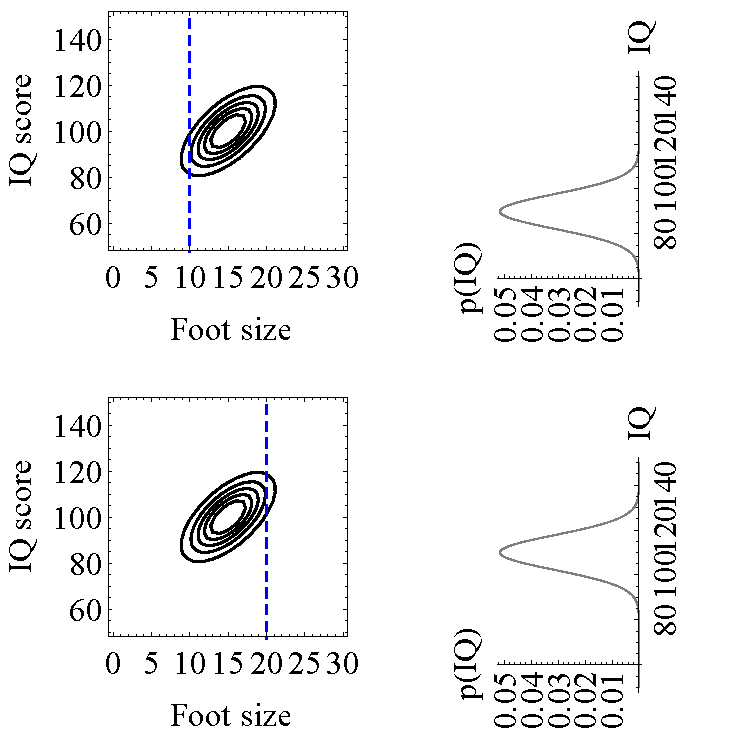
\includegraphics{Probability_footSizeIntelligenceConditional.pdf}}
\caption{The dashed blue lines indicate the new event space in each case. The height walked following these lines is related to the magnitude of the conditional distributions shown on the right.}\label{fig:Probability_footSizeIntelligenceConditional}
\end{figure}

We can also use (\ref{eq:Probability_conditionalProbability}) to allow us to calculate the conditional distribution of literacy scores for individuals after we have measured their shoe size. The only difference with the discrete example is that we now have to use an integral to work out the marginal probability for foot size; the denominator of (\ref{eq:Probability_conditionalProbability}). Figure \ref{fig:Probability_footSizeIntelligenceConditional} shows the conditional distributions traced out when we measure an individual's foot size to be 10cm and 20cm respectively. The blue dashed lines show the new event space, since we have lost our uncertainty over foot size in each of the cases. Therefore the heights traversed on the walk along these lines of constant foot size indicate the relative likelihood of different values of literacy scores. 

Add a stick man diagram.

\section{Higher dimensional probability densities: no harder than 2-D, just looks it!}
Now that we are equipped with the tools to calculate marginal and conditional distributions in two dimensions, we can use these to work with probability distributions that depend on any number of variables. Although formulae appear more complex, this is really just a result of having to keep track of each individual variable.

Imagine that we are told that there is another horse C, which comes from the same stable as horses A and B, which will compete in a third race, on the same day as the other two. This probability distribution could be represented by a 3-dimensional array, or alternatively as two separate tables of the same form as table \ref{tab:Probability_coinBiased}, one for each outcome for horse C's race. We could write this probability distribution as before, but with a third random variable $p(X_A,X_B,X_C)$. If we were only interested in the result of horses A and B, we can define a vector $\boldsymbol{Z}=(X_A,X_B)$, meaning that we could write our density as $p(\boldsymbol{Z},X_C)$. We can then just apply the same rule as before (in (\ref{eq:Probability_marginalDiscreteProbabilityTwoDimensions})) to get the marginal density, because our notation makes it look '2-dimensional':

\begin{equation}\label{eq:Probability_3DDiscreteHorsesExample}
\begin{align}
p(X_A,X_B) = p(\boldsymbol{Z}) &= \sum\limits_{X_C=0}^{1} p(\boldsymbol{Z},X_C)\\
&= p(\boldsymbol{Z},0) + (\boldsymbol{Z},1)
\end{align}
\end{equation}

If we wanted to work out the new probabilities of the two horses winning \textit{conditional} on the fact that horse C has won, we can simply use our 'two-dimensional' notation, and equation (\ref{eq:Probability_conditionalProbability}):

\begin{equation}
\begin{align}
&p(X_A, X_B|X_C=1) = \frac{p(X_A,X_B,X_C=1)}{p(X_C=1)}\\
&= \frac{p(X_A,X_B,X_C=1)}{p(1,1,X_C=1) + p(1,0,X_C=1) + p(0,1,X_C=1) + p(0,0,X_C=1)}
\end{align}
\end{equation}

Notice now however, that the denominator $p(X_C=1)$; representing the marginal probability of horse C winning is actually obtained by a sum over all the four possible ways this can occur: A and B winning, A winning and B not, B winning and A not, and finally both A and B losing\footnote{I have shortened the notation to allow all the outcomes to be shown on a single line, so $p(X_A=1,X_B=1,X_C)=p(1,1,X_C)$, for example.}.

For another example, suppose that we have a continuous posterior density that is defined in terms of three person-specific variables, $p(IQ,FS,W)$; where $W$ represents the weight of an individual. If we wish to determine the posterior solely as a function of $IQ$ and $FS$, then we start by defining the parameter vector $\boldsymbol{\theta} = (IQ,FS)$, meaning we are left with $p(\boldsymbol{\theta},W)$. Note that all we have done is defined a new composite variable, $\boldsymbol{\theta}$. Now our density is of the '2-dimensional' form shown in (\ref{eq:Probability_marginalContinuousProbabilityTwoDimensions}), and we can apply this relation:\\

\begin{equation}\label{eq:Probability_higherDimensionalMarginal}
\begin{align}
p(IQ,FS) &= p(\boldsymbol{\theta})\\
&= \int\limits_{All\; W} p(\boldsymbol{\theta},W)\mathrm{d}W
\end{align}
\end{equation}

If we wish to find the marginal distribution for $IQ$ \textit{only}, then all we do is integrate the resultant distribution in (\ref{eq:Probability_higherDimensionalMarginal}) with respect to $FS$.

We can use exactly the same trick to calculate the \textit{conditional} density of $IQ$ and $FS$, conditional on observing weight:

\begin{equation}\label{eq:Probability_higherDimensionsConditional}
\begin{align}
p(IQ,FS|W) &= p(\boldsymbol{\theta}|W)\\
&= \frac{p(\boldsymbol{\theta},W)}{p(W)}
\end{align}
\end{equation}

In (\ref{eq:Probability_higherDimensionsConditional}), we have used (\ref{eq:Probability_conditionalProbability}) to arrive at the second line.

Finally, note that combining all parameters of interest into a single parameter vector $\boldsymbol{\theta}$ allows us to calculate \textit{marginal} and \textit{conditional} distributions for probability distributions that depend on an arbitrary number of parameters.

\section{Independence}\label{sec:Probability_independence}
If we think that there is a relationship between two random variables, then we say that they are \textit{dependent}. This does not necessarily mean \textit{causal} dependence, as it is sometimes supposed, in that the behaviour of variable $A$ affects the outcome of variable $B$. What it really means is that the value taken on by $A$ is informative for predicting $B$. 

An example of dependence might be the \textit{colour} and \textit{suit} of a playing card. If we are told that the colour of a playing card is $red$, this means that our other variable \textit{suit} is constrained to be either \textit{hearts} or \textit{diamonds}. In this case, knowing with certainty the value of the first variable, \textit{colour}, helps us to narrow down the list of outcomes of the second variable, \textit{suit} (see figure \ref{fig:Probability_IndependenceCards}).

\begin{figure}
\centering
\scalebox{0.3} 
{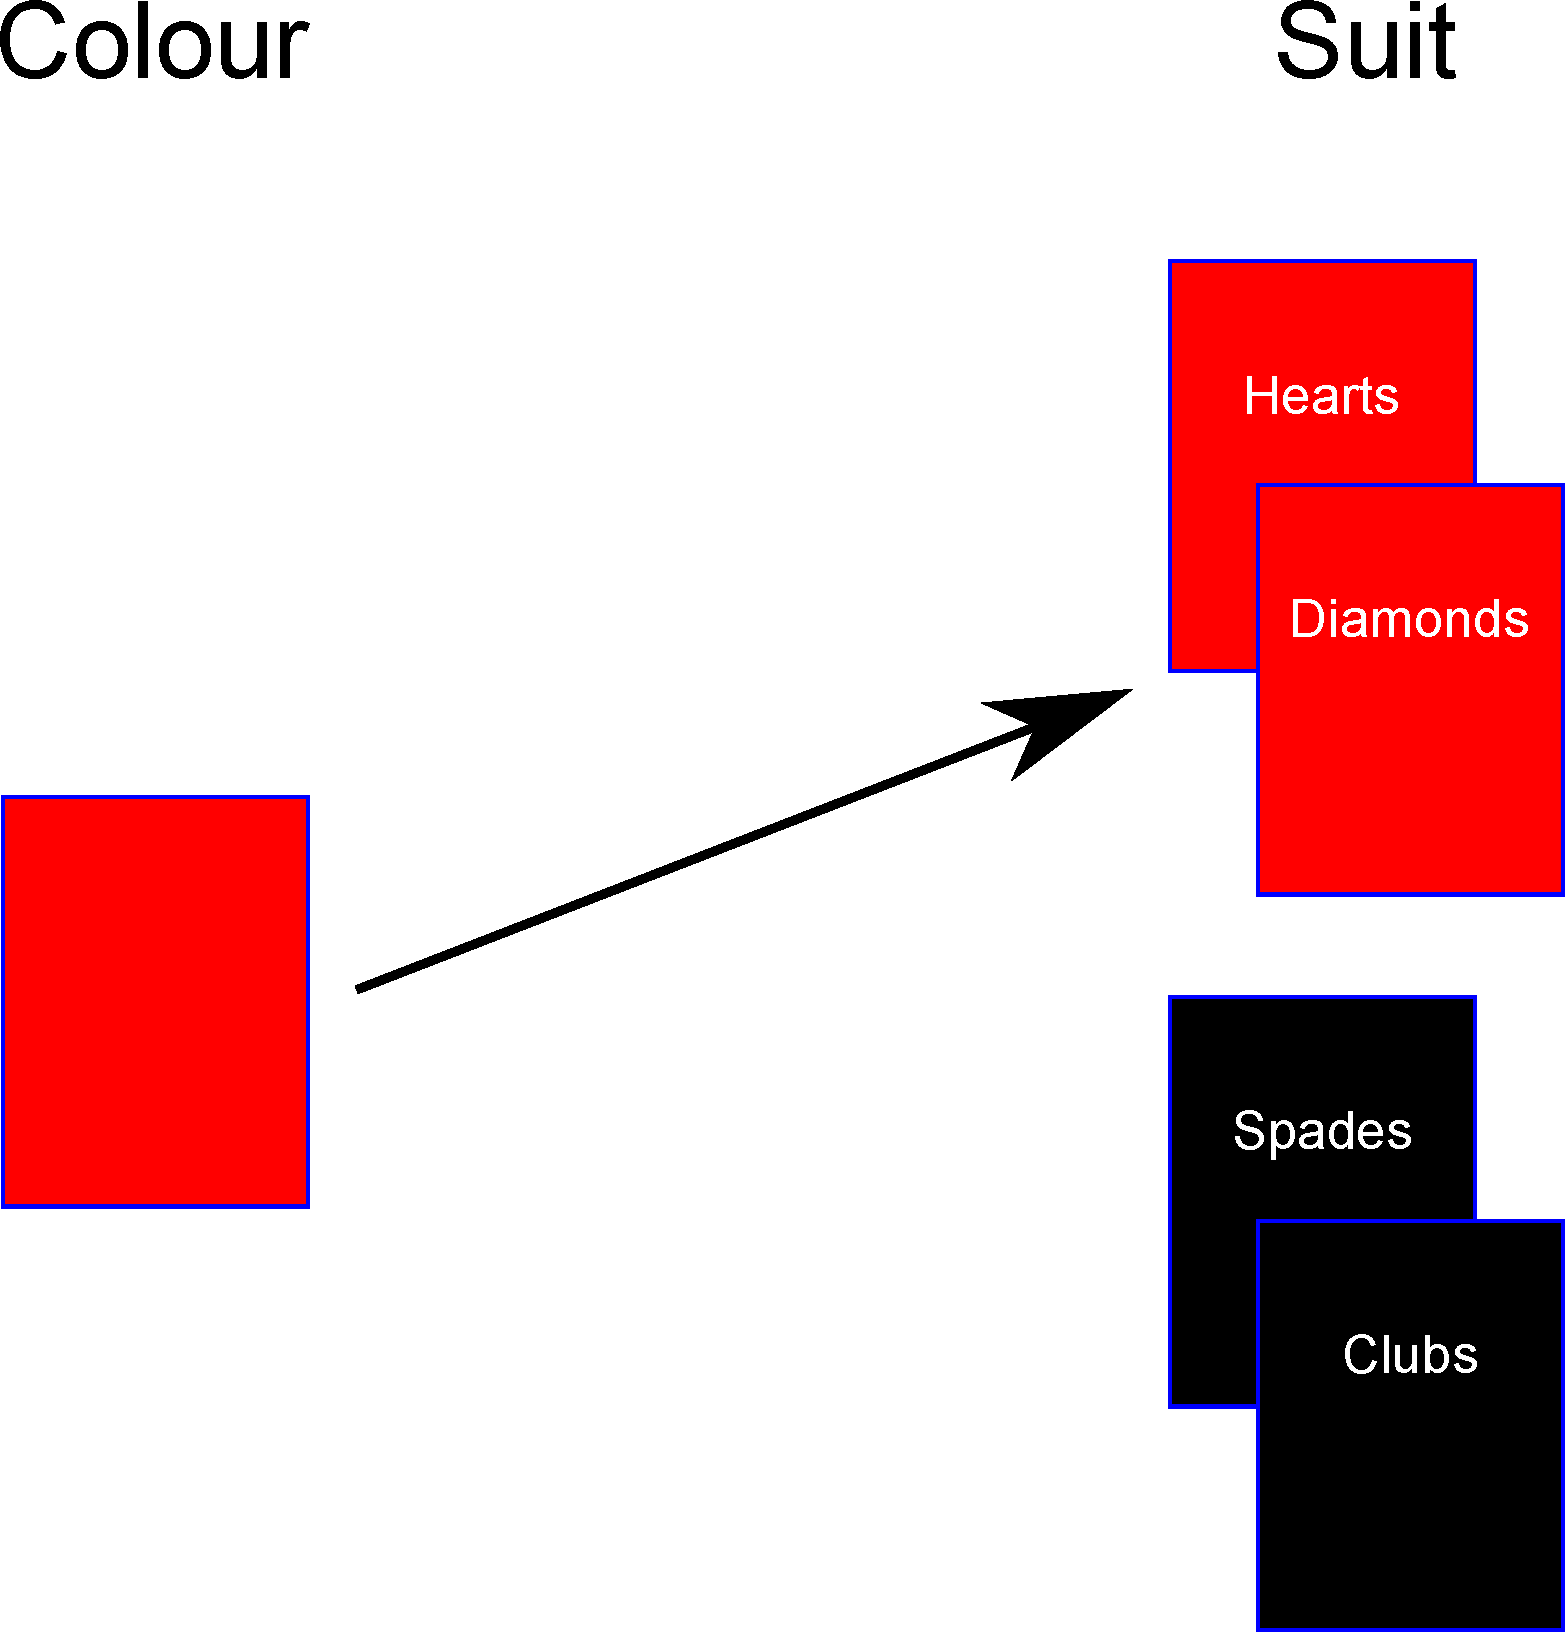
\includegraphics{Probability_IndependenceCards.pdf}}
\caption{Knowledge of the colour of a card provides information about the suit of the card. The colour and suit of a card are \textit{dependent}.}\label{fig:Probability_IndependenceCards}
\end{figure}

Another example of dependent variables, is the weather outside and the suntan of a particular, vein, individual\footnote{Discounting sunbeds.}. If it is sunny, then we assume it is more likely that an individual is tanned. Whereas, if the weather is cloudy, it is less so.

If two variables, $A$ and $B$ are \textit{disjoint}, then if one occurs, then the other cannot. In this case, it is often mistakenly believed that the variables are \textit{independent}, although this is very much not the case (see the left hand panel of figure \ref{fig:Probability_VennIndependence}). In this case, knowledge of variable $A$, provides significant information about variable $B$. If $A$ occurs, then we know for \textit{certain} that $B$ cannot!

\begin{figure}
\centering
\scalebox{0.4} 
{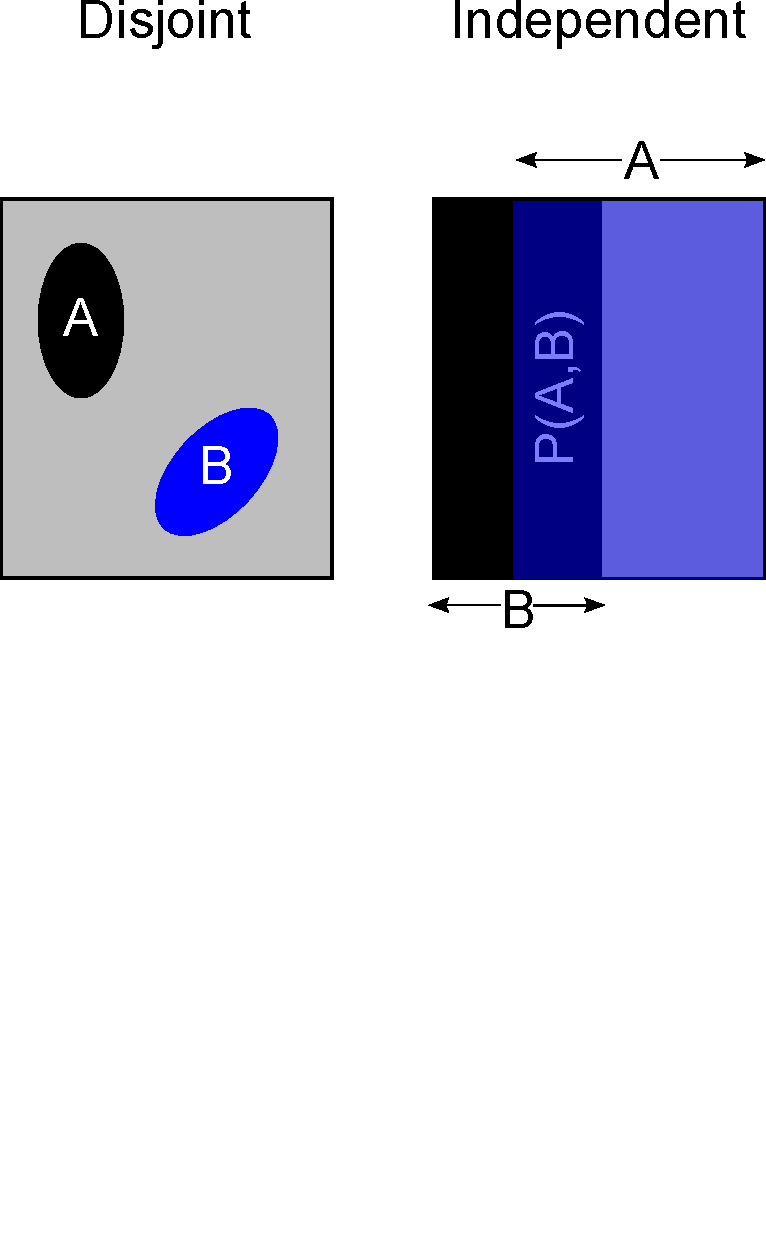
\includegraphics{Probability_VennIndependence.pdf}}
\caption{Venn diagram depictions of left: disjoint, and right: independent, events $A$ and $B$.}\label{fig:Probability_VennIndependence}
\end{figure}

By contrast, if two events are \textit{independent}, then knowledge of $B$ provides no additional information on $A$. Mathematically, this means that the conditional probability of $A$ is equal to the marginal:

\begin{equation}\label{eq:Probability_independentConditionalEqualMarginal}
p(A|B) = p(A)
\end{equation}

Using our conditional probability rule given in (\ref{eq:Probability_conditionalProbability}), we can then use this to rewrite the above as:

\begin{equation}\label{eq:Probability_independentConditionalEqualMarginal1}
\frac{p(A,B)}{p(B)} = p(A)
\end{equation}

In words, the ratio of the area of overlap between $A$ and $B$ to the area of $B$, is the same as the overall probability of $A$ (see the right hand panel of figure \ref{fig:Probability_VennIndependence}). This makes intuitive sense, since uncovering that $B$ has occurred (being in $B$) should result in no change to the probability of $A$ occurring (now $p(A|B)$).

Another way of stating independence that is commonly used, is obtained by multiplying (\ref{eq:Probability_independentConditionalEqualMarginal}) by its denominator:

\begin{equation}\label{eq:Probability_independentMultiplicationForm}
p(A,B) = p(A)\times p(B)
\end{equation}

To make this idea more concrete, we can think again of our horses example. Imagine that now are are considering two horses C and D, that come from separate stables, and race on different days. Using historical race results we have come up with the probability distribution shown in table \ref{tab:Probability_horsesIndependent}. 

We can use this table to test whether or not the results for the two horses are independent using (\ref{eq:Probability_independentMultiplicationForm}). We should be able to get the joint probabilities of both C and D winning from multiplying together the individual marginal densities:

\begin{equation}
\begin{align}
p(X_C=1,X_D=1) &= 0.3\\
&= p(X_C=1) \times p(X_D=1) 
&= 0.6 \times 0.5 = 0.3
\end{align}
\end{equation}

which we see is true. We could similarly also validate this by checking the other three joint outcomes in the table, and find that this is the case.

\begin{table}[htbp]
  \centering
    \begin{tabular}{rrccr}
    \toprule
          &       & \multicolumn{2}{c}{\textbf{horse C}} &  \\
    \midrule
          &       & \textbf{0} & \textbf{1} & \multicolumn{1}{c}{\textbf{$Pr(X_D)$}} \\
    \multicolumn{1}{c}{\textbf{horse D}} & \multicolumn{1}{c}{\textbf{0}} & 0.2   & 0.3   & \multicolumn{1}{c}{\textbf{0.5}} \\
    \multicolumn{1}{c}{} & \multicolumn{1}{c}{\textbf{1}} & 0.2   & 0.3   & \multicolumn{1}{c}{\textbf{0.5}} \\
          & \multicolumn{1}{c}{\textbf{$Pr(X_C)$}} & \textbf{0.4} & \textbf{0.6} & \multicolumn{1}{c}{} \\
    \bottomrule
    \end{tabular}%
  \caption{The probability distribution for horses C and D. The marginal distribution of horses C and D are achieved by summing the values in each column or row respectively.}\label{tab:Probability_horsesIndependent}%
\end{table}%

\subsection{Conditional independence}\label{sec:Probability_conditionalIndependence}
In statistics we often come across situations where we suppose that observations are \textit{conditionally} independent. This is often swept under the carpet, and in discussion authors (falsely) state that the observations are \textit{independent}. Suppose that we work for the WHO, as an epidemiologist, and are interested in estimating the proportion of obese individuals within a distinct urban area. Within this are, we can suppose that there exists a true proportion of this condition, $\theta$. Suppose we select an individual uniformly at random from this population, and record their status, $X_1$, for this disorder. We then pick another individual, and record their status, calling it $X_2$. If we knew $\theta$, then we might suppose that the outcomes of these two picks are independent \textit{conditional} on this overall parameter. In other words, the outcome of the first sampling provides us \textit{no} further information on the disorder status of the second.

This conditional independence property has frequently be represented in diagrammatic form of the type shown in figure \ref{fig:Probability_conditionalIndependence}. The arrows represent a dependency. When viewed in this light we see that it is incorrect to view the disease statuses of individuals 1 and 2 as \textit{fully} independent, since they are linked through a joint dependence on $\theta$. However, note that there is no direct arrow joining $X_1$ and $X_2$; this means that the random variables are \textit{conditionally} independent, when we allow for a joint dependence on $\theta$. 

\begin{figure}
\centering
\scalebox{0.4} 
{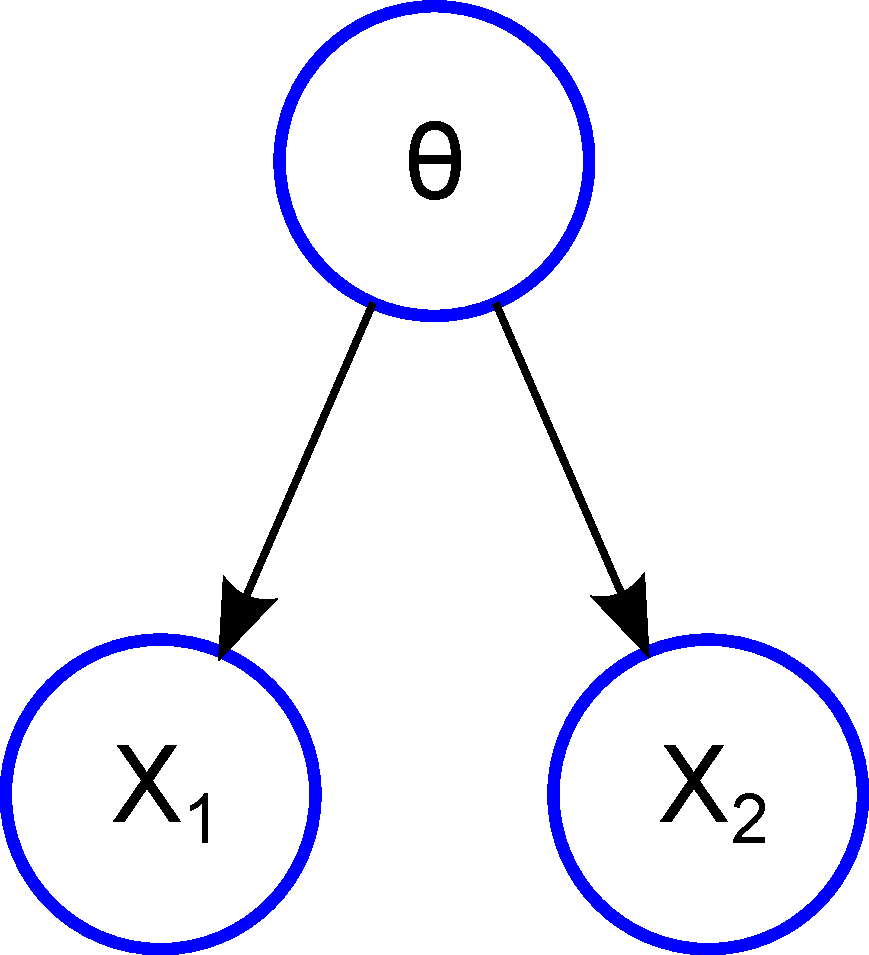
\includegraphics{Probability_conditionalIndependence.pdf}}
\caption{A diagrammatic depiction of conditional independence.}\label{fig:Probability_conditionalIndependence}
\end{figure}

\section{Central Limit Theorems}\label{sec:Probability_CLT}
Life is rarely simple, and in stating statistical models of phenomena we are attempting to at best, \textit{approximate} what is actually happening. In this environment, anything that brings a degree of certainty and coherence to our models is most welcome. 

Imagine that we are tasked with coming up with a model of probability for the \textit{mean} IQ test score in a particular school. Furthermore, as a simplification, we imagine that IQ is constrained to lie in the range $\left[0,300\right]$, and we believe that a reasonable probability distribution for an individual's test score is uniform on this range\footnote{Albeit this isn't a particularly good model, but suspend your disbelief for this thought experiment.} (see figure \ref{fig:Probability_CLTNormalSum}). We also suppose that individuals' scores are independent of one another.

Before we consider a sample size of $N$, we imagine that we only have a sample of two individuals, and we are asked to describe the distribution for the mean of their scores. If we use our assumption of uniformity, we might then ask, whether any mean scores are more likely than others, or are \textit{all} values equally likely, as per the individual case? We start by considering the extremes: there is only one way to achieve a mean test score of 300; both individuals would have to had scored 300. Similarly, to obtain a mean of 0, both individuals must score 0. However, consider obtaining a mean of 150. This could have been obtained with a number\footnote{Technically an infinity.} of combinations of scores, for example $\left(score_A,score_B\right)=$: $\left(150,150\right),\;\left(100,200\right),\;\left(125,175\right)$. Intuitively, there are many more ways of obtaining moderate values for the sample mean, that there are for the extremes. 

This tendency towards the centre increases the more values we sum over, since in order to get extreme values we would require \textit{more} individual scores to be simultaneously extreme; which is less likely. We can see this increasing central-tendency in figure \ref{fig:Probability_CLTNormalSum}, as the number of points being summed over increases.

However, we also see another tendency of the probability densities: \textit{an increasingly good fit of the normal distribution to these sample averages.} This approximation, it turns out, becomes \textit{exact} in the limit that we have an infinite sample, and is known as the \textit{Central Limit Theorem}. Although for our purposes, it will often be practically-exact if the sample size is sufficiently large. 

There are in fact a number of central limit theorems, of which we have only exposed you to the one for the average of independent, identically-distributed random variables\footnote{Known as the Lindeberg-Levy CLT. \textbf{Note: need an accent on the e.}}. However, what is important for you to note is that, whenever we have a number of factors, which additively result in an outcome, then an assumption of normality may be reasonable.

For example, there is an argument which would suggest that an individual's intelligence is the result of a number of factors including: un-bringing, genetics, life-experience, and health amongst others. Hence, we might tentatively propose that an individual's test score picked at random from the population would actually be normally-distributed! This is why I earlier discussed that the assumption that individuals' test scores were uniform might not be reasonable.

\begin{figure}
\centering
\scalebox{0.4} 
{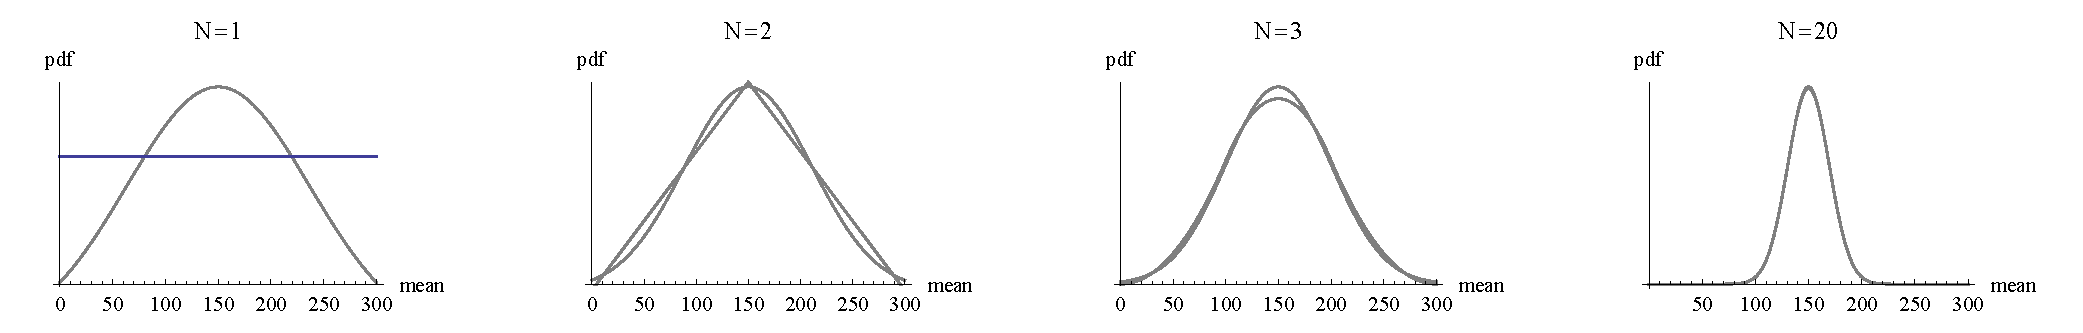
\includegraphics{Probability_CLTNormalSum.pdf}}
\caption{The convergence to a normal distribution for the mean of a sum of uniform distributions for IQ. The pdf for the average is shown in blue, with a normal distribution of the same mean and variance indicated in grey.}\label{fig:Probability_CLTNormalSum}
\end{figure}

\section{The Bayesian formula}\label{sec:Probability_BayesianFormula}
We first of all rewrite the conditional probability formula (\ref{eq:Probability_conditionalProbability}), regarding the probability of event A occurring, \textit{given} that event B has occurred:

\begin{equation}\label{eq:Probability_conditionalProbabilityAB}
p(A|B) = \frac{p(A,B)}{p(B)}
\end{equation}

However, we could also swap A and B around leading to the following for the probability of B \textit{given} that A has already occurred:

\begin{equation}\label{eq:Probability_conditionalProbabilityBA}
p(B|A) = \frac{p(B,A)}{p(A)}
\end{equation}

We however reason from the Venn diagram in figure \ref{fig:Probability_Venn}, that the overlap region of $p(A,B)$ really translated means, the probability of A \textit{and} B occurring. This means that this is exactly the same as the reverse; the probability of B \textit{and} A coinciding, $p(B,A)$. We can therefore rearrange (\ref{eq:Probability_conditionalProbabilityBA}) for this joint probability:

\begin{equation}\label{eq:Probability_jointConditionalProbability}
p(A,B) = p(B|A)\times p(A)
\end{equation}

We can use (\ref{eq:Probability_jointConditionalProbability}) to break down the probability of both A and B occurring into two steps. Firstly, for this to happen we require that A \textit{must} happen, with its corresponding probability $p(A)$. Then for both to occur, we straightforwardly require the probability of B occurring, \textit{given} that A has already occurred, which is given by $p(B|A)$. This reasoning provides a little intuition as to the workings of the conditional probability law that we wrote down in (\ref{eq:Probability_conditionalProbability}).

We can finally substitute (\ref{eq:Probability_jointConditionalProbability}) into the numerator of the fraction in (\ref{eq:Probability_conditionalProbabilityAB}), to yield the famous Bayesian formula!

\begin{equation}\label{eq:Probability_BayesianFormula}
p(A|B) = \frac{p(B|A)\times p(A)}{p(B)}
\end{equation}

The Bayesian formula importantly tells us how to correctly convert from $p(B|A)$ to its inverse $p(A|B)$, which is central to Bayesian statistics.

\subsection{The intuition behind the formula}
If we multiply both sides of (\ref{eq:Probability_BayesianFormula}) by $p(B)$, we arrive at the following alternative statement of Bayes' rule:

\begin{equation}\label{eq:Probability_BayesianIntuition}
p(A|B)\times p(B) = p(B|A)\times p(A) \;\;\;[= p(A,B)]
\end{equation}

In (\ref{eq:Probability_BayesianIntuition}), we have added the final part in square parentheses due to the reasoning of section \ref{sec:Probability_BayesianFormula}, that both sides are equivalent to the joint probability of A and B.

What the relation (\ref{eq:Probability_BayesianIntuition}) tells us however, is that there are two ways of arriving at this joint probability (see figure \ref{fig:Probability_BayesianIntuition}). The first way is given by the left hand side, and is due to B occurring, with probability $p(B)$, followed by A \textit{given} that B has occurred, with probability $p(A|B)$. An exactly equivalent way route to both A and B occurring is given by the right hand side of the leftmost equals sign. Here we require that A occurs first, with probability $p(A)$, followed by B \textit{given} that A has occurred, with probability $p(B|A)$.

\begin{figure}
\centering
\scalebox{0.4} 
{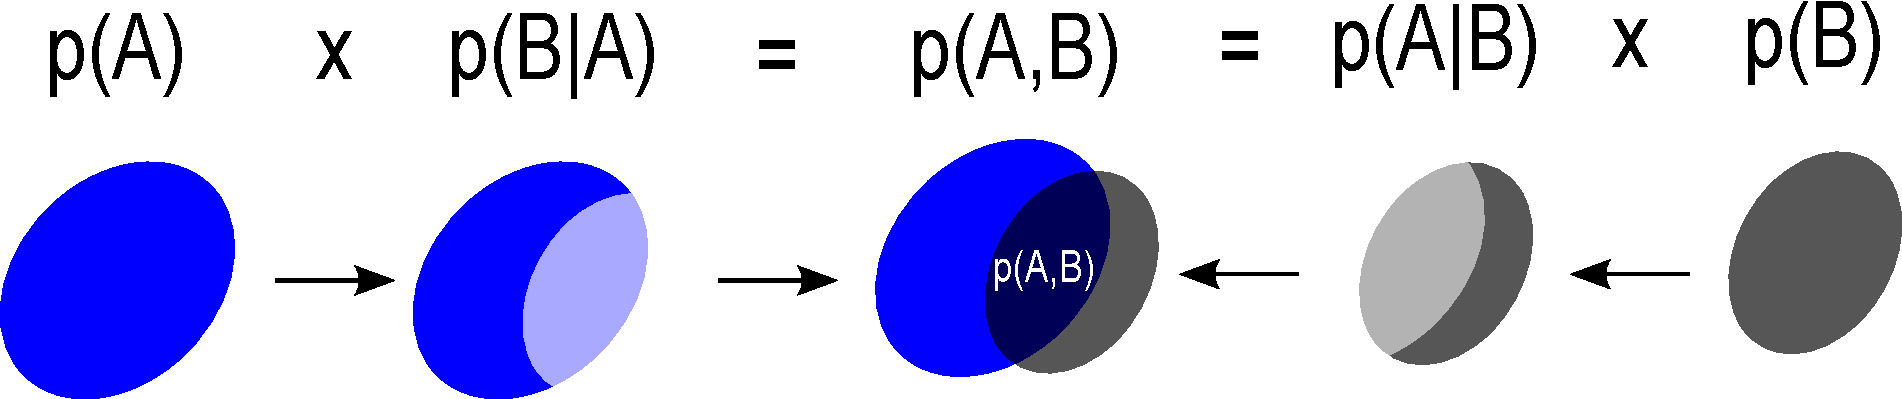
\includegraphics{Probability_BayesianIntuition.pdf}}
\caption{The two ways of arriving at the joint probability $p(A,B)$; providing some intuition behind Bayes' rule.}\label{fig:Probability_BayesianIntuition}
\end{figure}

\subsection{Breast cancer screeing}
Let's now make this discussion more concrete by means of an example. Let's imagine that we are an oncology doctor, working in breast cancer diagnosis. We suppose that out of all women aged forty who participate in screenings, about 1\% of them will have breast cancer at the time of testing. We suppose that the screening process is relatively robust, and it is known that for women who have breast cancer, the tests will indicate a positive result 80\% of the time. However, there is also the risk of false-positives, with 10\% of women without breast cancer also testing positive\footnote{I am not necessarily indicating clinically-up-to-date values, more I am using these example values to indicate the importance of reducing false-positives of any medical-test.}.

We now suppose that we are in the position where a woman has tested positive. What we would like to do, is work out the probability that she has breast cancer.

In the language of probability we would like to work out the conditional probability: $p(cancer|+ve)$. In words, the probability that she has breast cancer, \textit{given} that she has tested positive. However, summarising the information we currently have in probability language: $p(cancer)=0.01$, $p(+ve|cancer)=0.8$, and finally $p(+ve|no\; cancer) = 0.1$. How can we proceed? Bayes' formula to the rescue:

\begin{equation}\label{eq:Probability_bayesBreastCancer}
\begin{align}
p(cancer|+ve) &= \frac{p(+ve|cancer)\times p(cancer)}{p(+ve)}\\
&= \frac{p(+ve|cancer)\times p(cancer)}{p(+ve,cancer)+p(+ve,no\;cancer)}\\
&= \frac{0.8\times 0.01}{0.8\times 0.01 + 0.1\times 0.99} \approx 0.08
\end{align}
\end{equation}

In (\ref{eq:Probability_bayesBreastCancer}), we got from the first line to the second by using (\ref{eq:Probability_marginalDiscreteProbabilityTwoDimensions}) to work out the marginal probability of an individual testing positive. The fact that the probability is so small is due to the risk of false positives (see video XXX for a fully-intuitive explanation of this), which produce many more positive diagnoses than the real-positives (because the risk of cancer is much lower than the probability of not having cancer).

\section{The Bayesian inference process from the Bayesian formula}
In Bayesian statistics we aim to use probability distributions to describe all components of our system. Our starting point is Bayes' rule:

\begin{equation}\label{eq:Probability_BayesianFormula1}
p(A|B) = \frac{p(B|A)\times p(A)}{p(B)}
\end{equation}

In statistics we are typically looking to estimate a number of parameters, which we will from now on call $\theta$, which represent a component of a statistical model which we build to represent a particular phenomenon. These parameters can be real (such as the proportion of individuals within a given population that have a disease), or mere abstractions (for example the scale parameter of a hyper-distribution).

In Bayesian statistics, we want to update our beliefs about values of a parameter \textit{given} that we have obtained a particular sample of data. Being Bayesians, we would like to represent these beliefs via a probability distribution, which we write as $p(\theta|data)$. However, we can use (\ref{eq:Probability_BayesianFormula1}), (if we associate $A$ with $\theta$, and $B$ with the \textit{data}) to write:

\begin{equation}\label{eq:Probability_BayesianInferenceFormula}
p(\theta|data) = \frac{p(data|\theta)\times p(\theta)}{p(data)}
\end{equation}

Although we have straightforwardly made two substitutions to arrive at (\ref{eq:Probability_BayesianInferenceFormula}) from (\ref{eq:Probability_BayesianFormula1}), what have we gained by doing so? Also, what exactly do the terms on the right hand side actually mean? Although we introduced these in chapter \ref{chap:subjectiveFrequentistBayes}, we will spend the next part of this book examining each of these components in detail.

\section{Chapter summary}
The reader should now have developed a working understanding of probability distributions. Of particular importance in Bayesian statistics are the concepts of marginal and conditional distributions introduced in sections \ref{sec:Probability_marginal} and \ref{sec:Probability_conditionalDistributionIntro} respectively. If you do not feel fully confident with probability distributions, do not fret, since we will have ample opportunity to work with these mathematical objects in the next part of the book, where we provide an in-depth discussion of the various elements of the central formula of Bayesian inference: Bayes' rule.

\section{Chapter outcomes}
The reader should now be familiar with the following concepts:
\begin{enumerate}
\item The conditions under which a probability distribution is valid.
\item The difference between probability and probability density.
\item Summary distribution measures, and how to calculate them.
\item Two-or-more dimensional probability distributions.
\item Marginal distributions and how to calculate them.
\item Conditional distributions and how to calculate them.
\item Independence,
\item Central Limit Theorems.
\item The Bayesian formula.
\end{enumerate}

\section{Problem set}
\subsection{The expected returns of a derivative}
The returns of a particular stock are thought to be well described by a log-normal distribution:

\begin{equation}
log(S_t) \sim N(\mu,\sigma)
\end{equation}

\subsubsection{What are the expected returns of the stock?}
\subsubsection{What are the variance in returns?}

The performance of a particular type of derivative is given by the following formula:
\begin{equation}
D_t = S_t^2
\end{equation}

\subsubsection{Would you expect the return to be equal to the mean of the original stock squared? If not, why not?}
Note to myself: the convexity of the squared function means that it is greater.
\subsubsection{What would be a fair price to pay for this derivative?}

An alternative stock is probabilistically related to the performance of $S_t$:

\begin{equation}
R_t \sim N(S^2,1)
\end{equation}

\subsubsection{What is a fair price to pay for this stock?}
\subsubsection{Which asset is more risky, $D_t$ or $R_t$?}

The data file XXX contains Stock return data for the stock $S_t$. A way to estimate the parameter is via a method known as \textit{method of moments}. Here, we might estimate the parameters $\mu$ and $\sigma$ by equating the sample mean and variance, to the \textit{population} quantities we believe our process abides by.

\subsubsection{Use \textit{method of moments} to estimate $\mu$ and $\sigma$. Note: this requires use of a computer with mathematical software, as analytic solutions aren't possible.}

\subsubsection{Compare the estimated model with the data.}
\subsubsection{Is the model a reasonable approximation to the data generating process?}
\subsubsection{If not, suggest a better alternative.}

\subsection{The boy or girl paradox\footnote{First introduced by Martin Gardner in 1959.}}
Suppose we are told the following information:

Mr Bayes has two children. The older child is a girl. What is the probability that both children are girls?
Mr Laplace has two children. At least one of the children is a girl. What is the probability that both children are girls?

\subsection{The Bayesian game show}
A game show presents contestants with four doors: behind one of the doors is a car worth \$1000; behind another is a forfeit whereby the contestant must pay \$500 out of their winnings thus far on the show. Behind the other two doors there is nothing.

The order of the game is thus:
\begin{enumerate}
\item The contestant chooses one of four doors.
\item The game show host opens one of the empty doors.
\item The contestant is given the option of changing their choice to one of the two remaining doors.
\item The contestant's final choice door is opened, either to their delight (a car!), dismay (a penalty), or indifference (nothing).
\end{enumerate}

Assuming that the contestant prefers less risk, what should they do?

If you are unsure as to how to proceed, why not simulate the game using a computer. The program should only be a few lines, and might provide you with some intuition as to what is happening.

\subsection{Blood doping}
Suppose as a benign omniscient observer, we tally up the historical cases where professional cyclists used/didn't-use blood doping, and either won or lost a particular race. This results in the probability distribution shown in table \ref{tab:Probability_PS_bloodDoping}.

\subsubsection{What is the probability that a professional cyclist wins a race?}
\subsubsection{What is the probability that a cyclist wins a race given that they have cheated?}
\subsubsection{What is the probability that a cyclist is cheating given that he wins?}

\begin{table}[htbp]
  \centering
    \begin{tabular}{ccc}
    \toprule
          & \textbf{Lost} & \textbf{Won} \\
    \midrule
    \textbf{Clean} & 0.7   & 0.05 \\
    \textbf{Doping} & 0.15  & 0.15 \\
    \bottomrule
    \end{tabular}%
    \caption{The historical probabilities of behaviour and outcome for professional cyclists.}
  \label{tab:Probability_PS_bloodDoping}%
\end{table}%

Now suppose that drug testing officials have a test which is relatively accurate in finding cheats. It accurately indicates a blood-doper 90\% of the time. However, it incorrectly indicates a positive for clean athletes 5\% of the time. 

Should the officials test all the athletes or only the winners, for the cases when:

\begin{enumerate}
\item They care only about the proportion of people correctly identified as dopers.
\item They want only to minimise the proportion of falsely accused athletes.
\item They care only about the \textit{number} of people correctly identified as dopers.
\item They care five times about the \textit{number} of people who are falsely identified as they do about the \textit{number} of people who are correctly identified as dopers.
\item What factor would make the officials choose the other group? (By factor, we mean the number 5 in the previous question.)
\end{enumerate}


\part{Understanding the Bayesian formula}\label{part:bayesianFormula}
\section{Part mission statement}
This part introduces the reader to the various elements of the Bayesian inference formula: the posterior, the likelihood, the prior and the denominator.

\section{Part goals}
The goal of Bayesian inference is to calculate the posterior distribution for parameters of interest. This distribution is the starting point for making decisions, and drawing conclusions about situations under examination. It is thus important to understand why this part of Bayes' formula is so useful, and hence we devote chapter \ref{chap:posterior} to this purpose. The first term on the right-hand-side of Bayes' formula that we encounter is the likelihood function, introduced in chapter \ref{chap:Likelihoods}. These functions/distributions allow for variance in the data, even if the parameters are fixed. This variance is what classical statisticians call sampling variation. Importantly, likelihood functions are not valid probability distributions, and are actually the inverse of what we desire. Bayes' rule essentially tells us how to invert these distributions in order to get our desired distributions - the posterior. However, in order to invert the likelihood, we need to specify the final piece of the puzzle - the prior distribution. This is a measure of our pre-data confidence across all the possible values of the parameter. We are required to specify this term, since Bayes' rule only tells us how to \textit{update} our beliefs, not how to specify them in the first place. Priors are without doubt the most controversial part of Bayesian inference, although as we have seen in chapter \ref{chap:subjectiveFrequentistBayes}, and we advocate in chapter \ref{chap:Prior}, this criticism is unwarranted. The final part of the formula - the denominator - is determined fully by our choice of likelihood and prior. However, this predetermination does not make out lives simple, and we shall see that the difficulty in evaluating this term, along with similar expressions, motivates the computational methods introduced in part \ref{part:computationalBayes}.

\chapter{The posterior - the goal of Bayesian inference}\label{chap:posterior}
\section{Chapter Mission statement}
At the end of this chapter the reader will understand the central importance, and use of the posterior probability distribution in Bayesian statistics.

Insert a graphic with the likelihood part of Bayes' formula circled, as in the equation shown below for the part highlighted in blue.

\begin{equation}
{\color{blue}p(\theta|data)} = \frac{p(data|\theta)\times p(\theta)}{p(data)}
\end{equation}\label{eq:Posterior_BayesHighlighted}

\section{Chapter goals}
Calculating the posterior distribution for a model's parameters is the focus of Bayesian analysis. This \textit{probability distribution} which results from the application of Bayes' rule (see \ref{eq:Posterior_BayesHighlighted}) can be used to infer the effects of given variables, to forecast, compare different models of phenomena, as well as test its own foundations! In order to do justice to the multitude of uses of the posterior distribution, it is necessary that the reader is familiar with the basics of probability distributions explained in chapter \ref{chap:subjectiveFrequentistBayes}. 

\section{Expressing uncertainty through the posterior probability distribution}\label{sec:Posterior_parameterUncertainty}
Unlike looking out the window, getting exam results, or playing a hand at blackjack, we frequently in inference never learn the \textit{true}\footnote{Whether a true value for a parameter actually exists we leave until section \ref{sec:Posterior_parametersExist}.} state of nature. The uncertainty here is both in the future and \textit{present}; the latter meaning we are unable to perfectly measure the state of the world today, and hence cannot hope to perfectly know the former.

A way of representing our ignorance, or uncertainty in a parameter's value is through probability distributions. For example, suppose that we wanted to know the proportion of individuals that would vote for the democrats in an upcoming election. We might, on the basis of past exit poll surveys, calculate a posterior\footnote{Via Bayes' rule - don't worry if you don't know how to do this, that is the goal of this whole first part!} uncertainty which is represented by the probability distribution which is shown in figure \ref{fig:Posterior_electionProportion}. 

\begin{figure}
\centering
\scalebox{0.5} 
{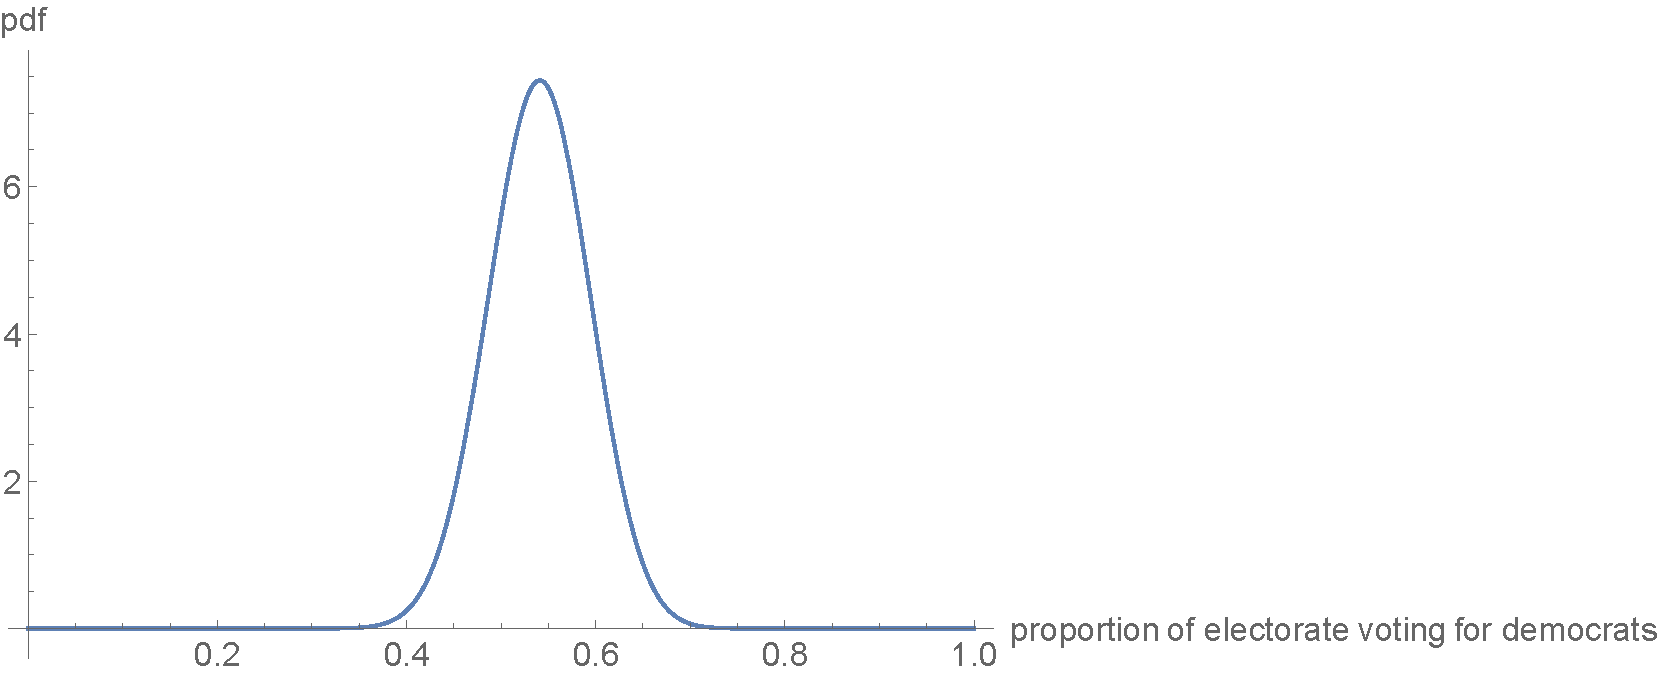
\includegraphics{Posterior_electionProportion.pdf}}
\caption{A probability distribution representing uncertainty over the proportion of the electorate that will vote for the Democrats in an upcoming election.}\label{fig:Posterior_electionProportion}
\end{figure}

How can we interpret the probability distribution shown in figure \ref{fig:Posterior_electionProportion}? And further, how can we use it to express our uncertainty to a non-mathematician? 

Often we describe a distribution by its summary characteristics. These are aspects of the distribution that we commonly want to know. For example, we normally want to know the \textit{mean} value of a parameter. This is a measure of central tendency of our estimates, that is essentially a weighted mean (where the weights are provided by the values of the probability density function). If we have the mathematical description of the distribution shown in figure \ref{fig:Posterior_electionProportion}, we can calculate this by simply finding its mean, by taking the expectation:

\begin{equation}
\mathbb{E}[\theta] = \int\limits_{0}^{1} p(\theta)\theta \mathrm{d}\theta = 54\%
\end{equation}

This provides a point estimate of the proportion of individuals - 54\% - that we expect to vote for the Democrats, which may be a useful piece of information to pass on to an interested party. 

A point estimate of the proportion of individuals that we expect to vote for the Democrats is not useful in itself, (and quite dangerous to pass on), without some measure of our inherent confidence/uncertainty in this particular value. One measure of uncertainty in a parameter's value is its variance:

\begin{equation}
var(\theta)=  \int\limits_{0}^{1} p(\theta)(\theta-\mathbb(E[\theta])^2 \mathrm{d}\theta
\end{equation}

In many cases, it is easier to understand the meaning of uncertainty if it is expressed in the same units as the mean, which we do by taking the square root of the variance, yielding 5.3\% for the case of figure \ref{fig:Posterior_electionProportion}. A larger variance indicates that we view a wider range of outcomes as being feasible. In this case, a wider variance would mean that we would be less surprised if the electorate voted in the Republican party. 

In sections \ref{sec:Posterior_HDI} and \ref{sec:Posterior_CPI} we will introduce other summary measures of distributions, that are also often presented in research articles, and books. However, the important thing to note is that all of these are derived from the posterior distribution for our parameters. 

Another example of the use of posteriors can be illustrated by a regression example. Suppose that we are investigating the effect of military participation on lifetime earnings\footnote{See Angrist's fantastic 1990 article for a detailed study of this effect for Vietnam war veterans \cite{angrist1990lifetime}.}. We suppose that the effect is, on average, negative due in part to the psychological stresses of warfare. We also suppose that the effect is can be modelled as being linear, and hence our relationship of interest can be represented as:

\begin{equation}\label{eq:Posterior_militaryParticipation}
LI_i = \alpha + \beta MP_i + \epsilon_i
\end{equation}

where we expect that $\beta$ is negative. Here $\epsilon_i$ represents the myriad of other factors that are important for determination of an individual's income.

If we formulate a Bayesian model, with a given prior and likelihood, then we might end up with a posterior density for $\beta$, that is shown in figure \ref{fig:Posterior_regressionMilitaryParticipation}. We can use this density to help us to calculate the posterior probability that the given parameter is in fact non-negative, by finding the area under the curve corresponding to $\beta\geq 0$ (shown as the shaded region in figure \ref{fig:Posterior_regressionMilitaryParticipation}), which we find in this case to be approximately 25\%. This suggests that we are not all that confident in the fact that the parameter is negative (at 75\%), and cannot reasonably go along with our hypothesis.

\begin{figure}
\centering
\scalebox{0.5} 
{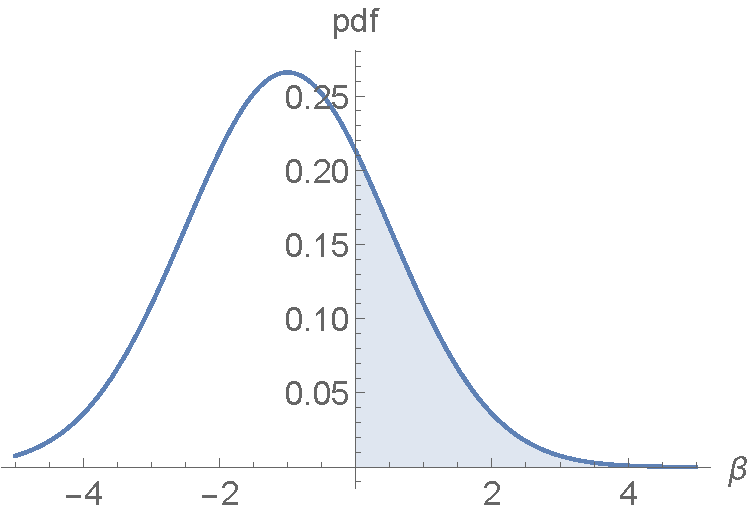
\includegraphics{Posterior_regressionMilitaryParticipation.pdf}}
\caption{An estimated posterior probability distribution for the parameter $\beta$ in (\ref{eq:Posterior_militaryParticipation}). The shaded region represents the posterior probability that the parameter is positive.}\label{fig:Posterior_regressionMilitaryParticipation}
\end{figure}

\subsection{Bayesian coastguard: introducing the prior and the posterior}
Imagine you are stationed in a radio control tower at the top of a steep cliff, in the midst of a stormy night. The tower received a distress call over radio from a ship - The Frequentasy - which has got engine trouble, somewhere out in the bay. It is your job to direct a search helicopter to rescue the poor sailors.

When you first receive the weak crackled radio signal, you are not made aware of their location. However, you know that the boat must be somewhere in the bay, less that 25km away from the tower, since this is the maximum possible range of the radio. Accordingly, you represent these views via the prior shown in the left hand panel of figure 1 (fairly flat prior in a circle from the tower, perhaps going down to zero gradually at 25km). The search area represented by this prior is currently far too wide for a rescue crew to reach the flagging ship in time!

In an attempt to improve the odds, you radio to the ship, and ask that they switch on their emergency transmitter. After radioing a number of times, you receive a weak signal, which you feed into the computer, resulting in a posterior probability density for the ship's location shown in the central panel of figure 1. (This panel shows a broadly peaked density along a line from the ship to the station, near a particular location 15km away).

The trouble is, the search area inferred from the aforementioned posterior is still wide. Luckily for the crew however, another nearby radio station has also picked up the signal, and they share this information with you. Finally, feeding this information into the computer, you obtain a final estimation of the ship's location, shown in the right hand panel of figure 1. 

Since there is only a small area of high density, you direct the rescue helicopter to search this area, and they find the find the captain and crew in time.

\begin{figure}
\centering
\scalebox{0.2} 
{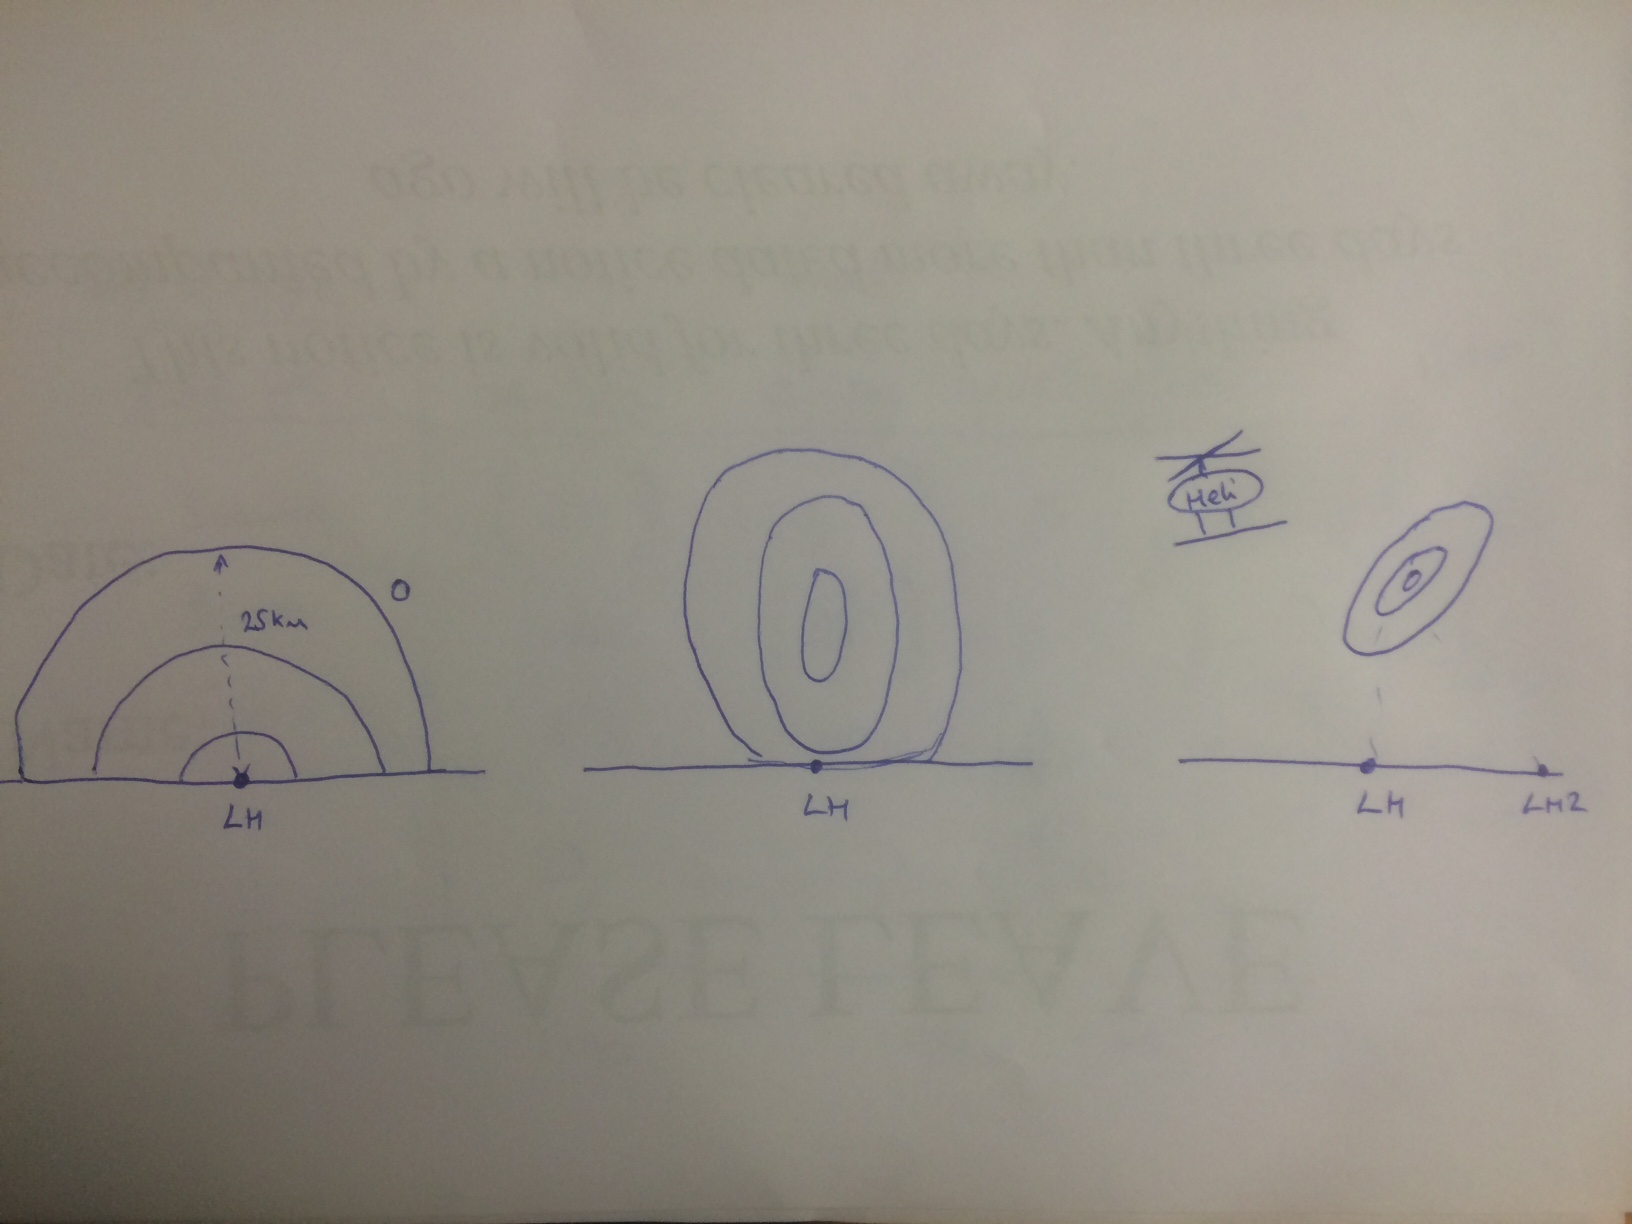
\includegraphics{Posterior_bayesianLighthouse.jpg}}
\caption{Three plots. Left hand plot is a contour plot of probability radiated symmetrically in a semi-circle away from the lighthouse, with the density declining to zero at 25km. The middle plot shows a contour plot of probability, with a higher density towards the centre of the diagram (here the densities are still relatively smooth, indicating high uncertainty). The final plot shows a definite peak in intensity around a particular point about 10km away from the coast, just right of centre. The different contours will be increasing shades of a particular colour.}\label{fig:Posterior_bayesianLighthouse}
\end{figure}

\subsection{Bayesian statistics: updating our pre-analysis uncertainty}
In Bayesian statistics the posterior distribution summarises the combination of our pre-study, and post-analysis knowledge about a given situation, and is used as the starting point for any further analysis or descriptions of our results. In order to calculate it, we need to choose a probability model, which in turn defines uncertain parameters, over which we place priors. The model also provides us with a \textit{likelihood} of the data we obtained. The priors and likelihoods are then combined in a certain way - using Bayes' rule - to yield the posterior distribution.

\begin{equation}
prior + data \rightarrow posterior
\end{equation}

In the Bayesian lighthouse example, we started off with a fairly wide prior, since we were quite uncertain of the boat's location. We then fed the data from the ships' emergency transmitter, along with the prior, into the computer - which uses Bayes' rule - to provide an updated estimate of the ship's location. We actually went through this process twice, to emphasise the fact that Bayes' rule can be used iteratively to update knowledge about an uncertain situation.

Statistical inference is useful whenever there is uncertainty regarding a parameter of interest. Bayesians use the posterior distribution, and various summaries of it, in order to describe the degree of uncertainty regarding a parameter. Before we delve too deep though, it is useful to take a step back, and ask the somewhat philosophical question, 'Do parameters actually exist?' 

\subsection{Do parameters actually exist and have a point value?}\label{sec:Posterior_parametersExist}
For Bayesians, the parameters of the system are taken to vary, whereas the known part of the system - the data - is taken as given. Whereas Frequentist statisticians view the unseen part of the system - the parameters of the probability model - as being fixed, whereas the known parts of the system - the data - as varying. Whether you agree with one of these views more than the other mainly comes down to how you want to interpret the parameters of a given statistical model. 

The Bayesian perspective on parameters can be viewed as having a duality of meaning. Either we view the parameters as truly \textit{varying}, or we view our knowledge about the parameters as imperfect. The fact that we will get different estimates of parameters from different studies can be taken to reflect either of these two views. Either we view the parameters of interest as varying - taking on different values in each of the samples we pick (see the bottom panel of figure \ref{fig:Posterior_manyWorldsDoParametersExist}). Alternatively, we can view our uncertainty over a parameter's value as the reason we will estimate slightly different values in different samples. This uncertainty is thought of as decreasing as we collect more data (see the middle panel of figure \ref{fig:Posterior_manyWorldsDoParametersExist}). Bayesians are more at ease with using parameters as a means to an end - taking them not as real immutable constants, but as tools from which to make inferences about a given situation.

The Frequentist perspective is less flexible, and assumes that these parameters are constant; alternatively representing the average of a long run - typically infinite number - of identical experiments. There are occasions when we might think that this is a reasonable assumption. For example, if our parameter represented the proportion of the electorate that voted for the Democrat party in the last election, or the probability that an individual taken at random from the UK population will have dyslexia. In both these examples, it is reasonable to assume that there is a \textit{true}, or fixed \textit{population} value of the parameter of question. Whilst the Frequentist view might be in some ways reasonable here, the Bayesian view easily extends here to encompass these two situations by assuming that we are uncertain about the value of these fixed parameters before we measure them, and using a probability distribution to represent this lack of perfect knowledge. 

However, there are circumstances when the Frequentist view runs into trouble. When we are estimating parameters of an arbitrarily complicated distribution, we normally do not view them as actually existing. Unless you view the universe as being built from mathematical building blocks\footnote{See \cite{tegmark2014our} for an interesting argument for this hypothesis}, then it seems incorrect to assert that a given parameter has any deeper existence than that with which we endow it. The less restrictive Bayesian perspective here seems more reasonable.

The Frequentist view of parameters as a limiting value of an average across an infinity of identically repeated experiments (see the top panel of figure \ref{fig:Posterior_manyWorldsDoParametersExist}) also runs into difficulty when we think about one-off events, such as the 2016 US Presidential Election result. Any parameter we wish to estimate about such an event cannot easily be existentially justified on these grounds, since elections cannot be rerun.


\begin{figure}
\centering
\scalebox{0.2} 
{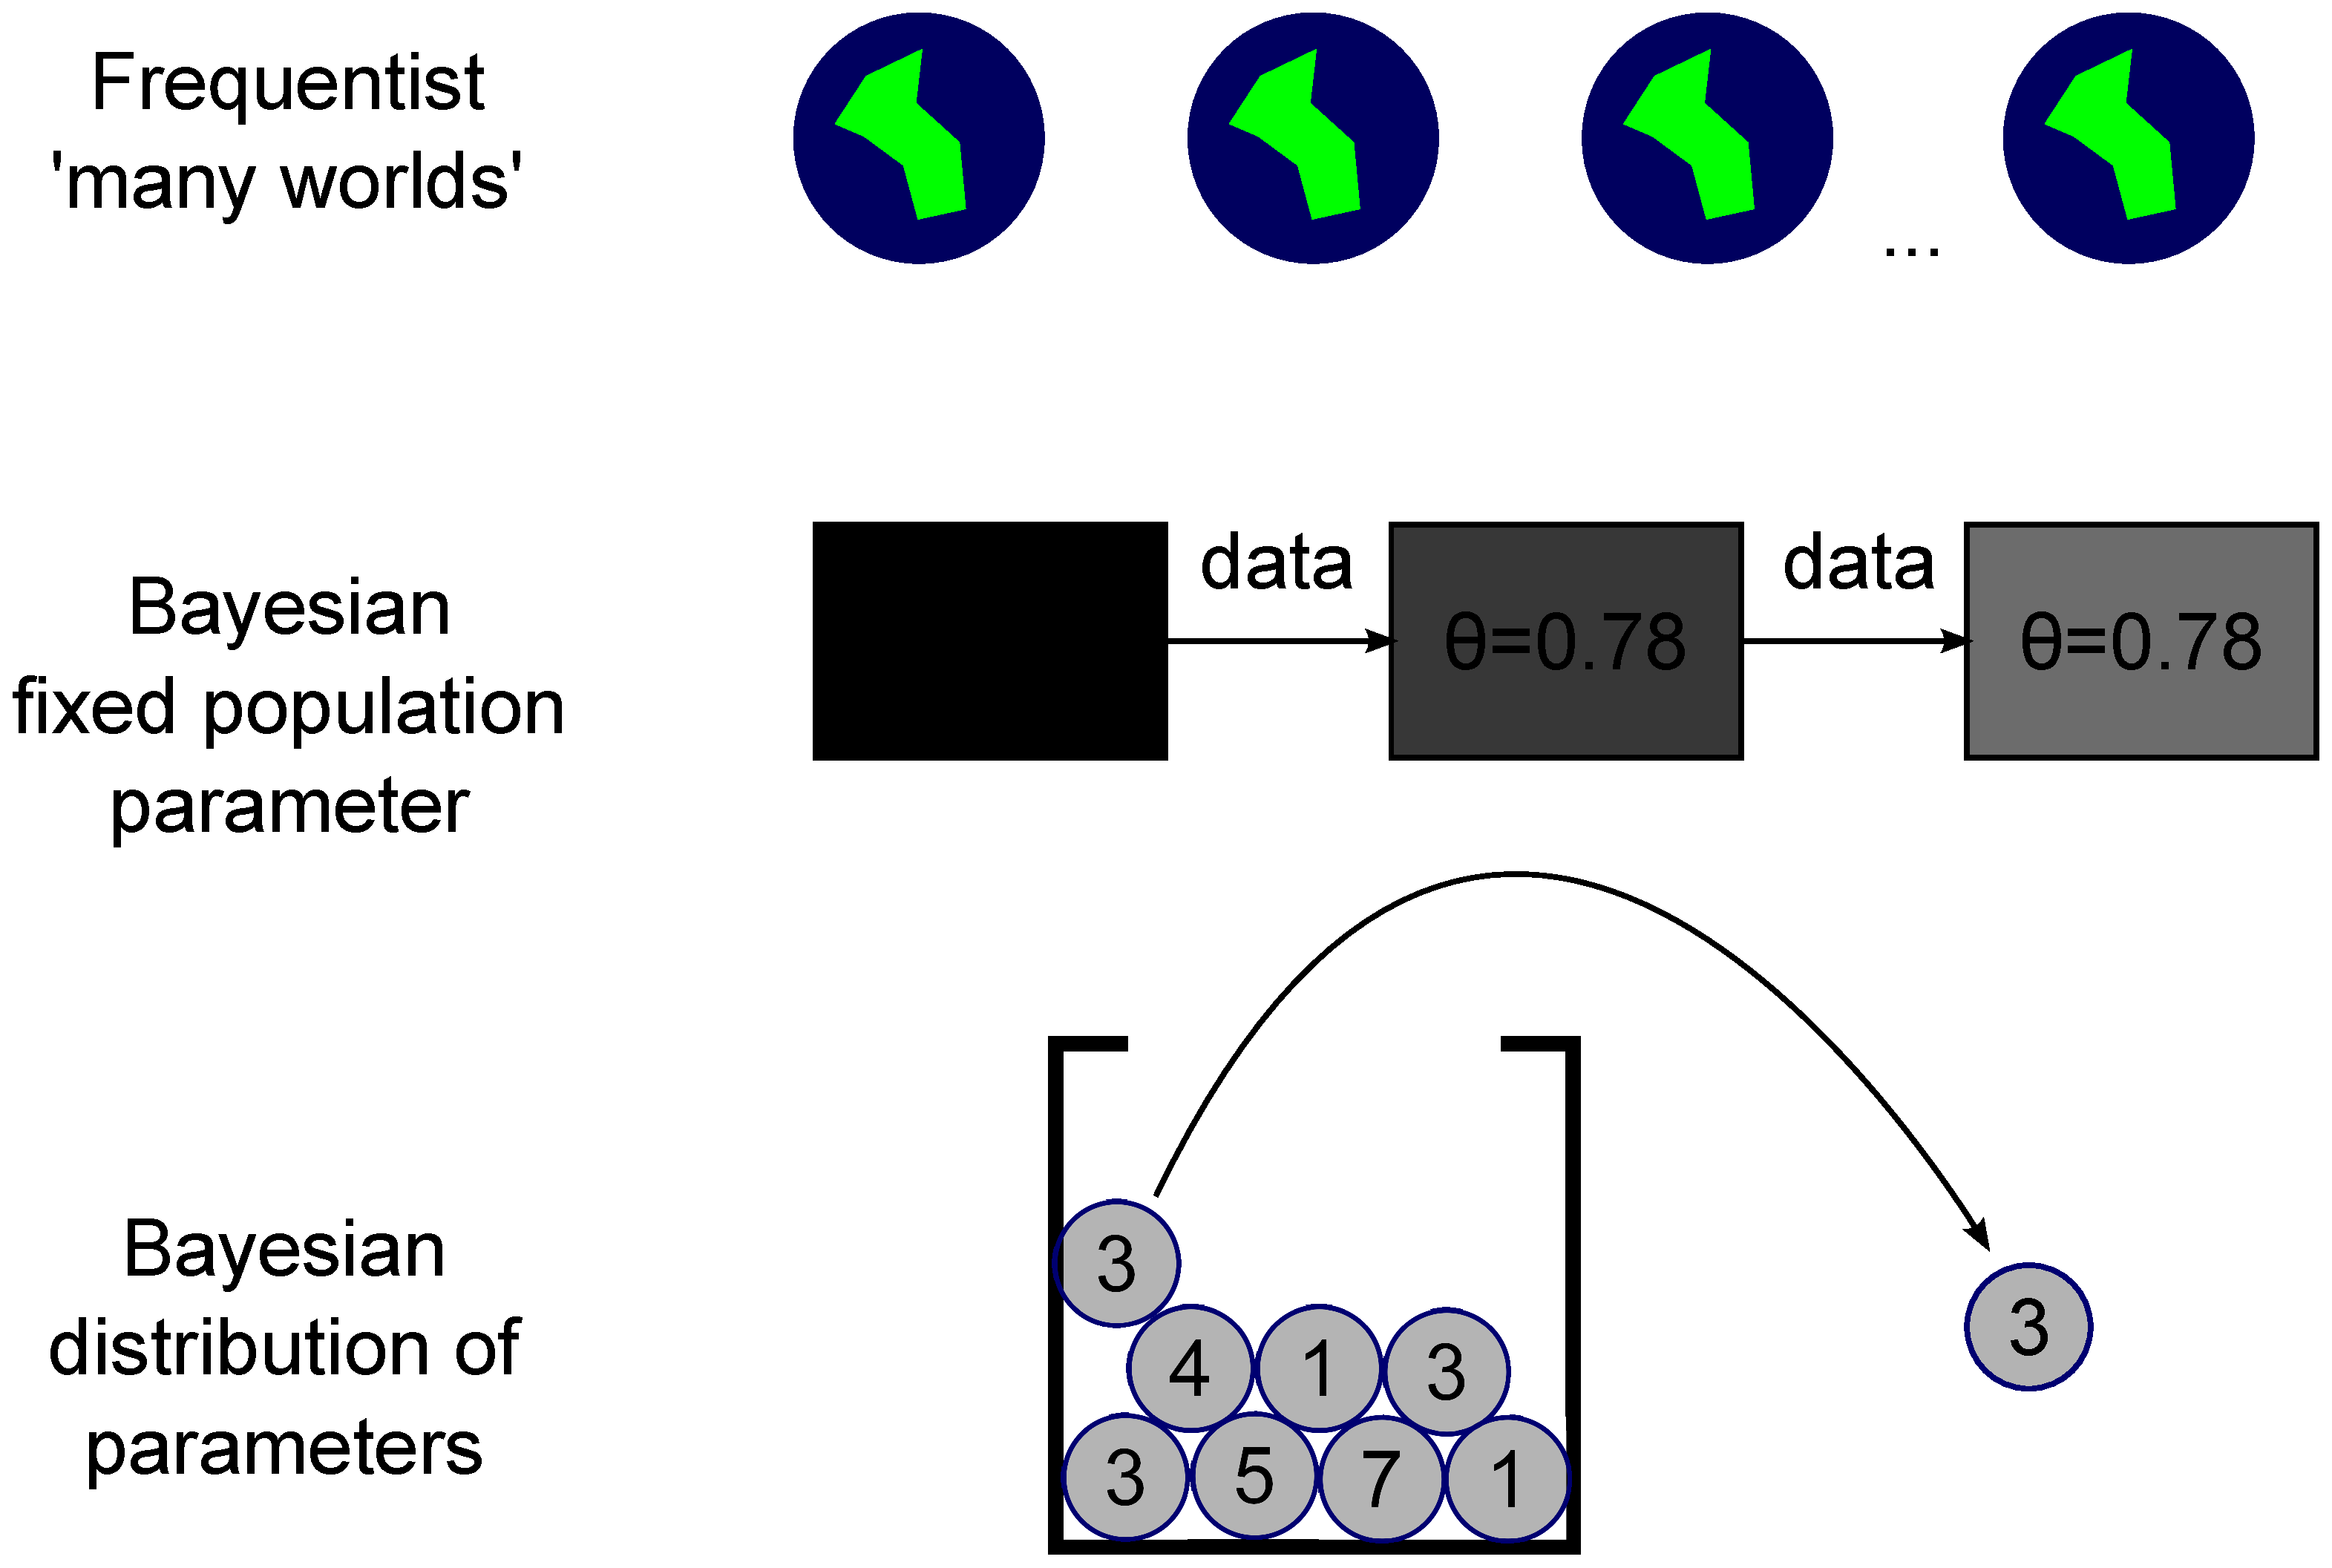
\includegraphics{Posterior_manyWorldsDoParametersExist.eps}}
\caption{The Frequentist and Bayesian perspectives on parameters.}\label{fig:Posterior_manyWorldsDoParametersExist}
\end{figure}

\subsection{Failings of the Frequentist confidence interval}\label{sec:Posterior_classicalConfidenceInterval}
A mainstay of the Frequentist estimation procedure is the \textit{confidence interval}. In empirical research we often see these intervals as stated for a given parameter (where for now we assume that the parameters are unknown and fixed). For example,

\textbf{'From our research, we concluded that the percentage of penguins with red tails, $RT$, has a 95\% confidence interval of $1\%\leq RT \leq 5\%$.'}

This is often incorrectly taken as having an implicit meaning, 'We are 95\% sure that the true percentage of penguins with red tails lies in the range of 1\% to 5\%.' However, what it actually captures is not uncertainty about the parameter in question, but about the interval we calculate. 

In the Frequentist paradigm we imagine that we are taking repeated samples from a population of interest, and for each of the samples, we estimate a confidence interval (see figure \ref{fig:Posterior_classicalConfidenceInterval}). A 95\% confidence interval means that across all of the intervals we calculate, the true value of the parameter will lie in this range 95\% of the time. 

\begin{figure}
\centering
\scalebox{0.4} 
{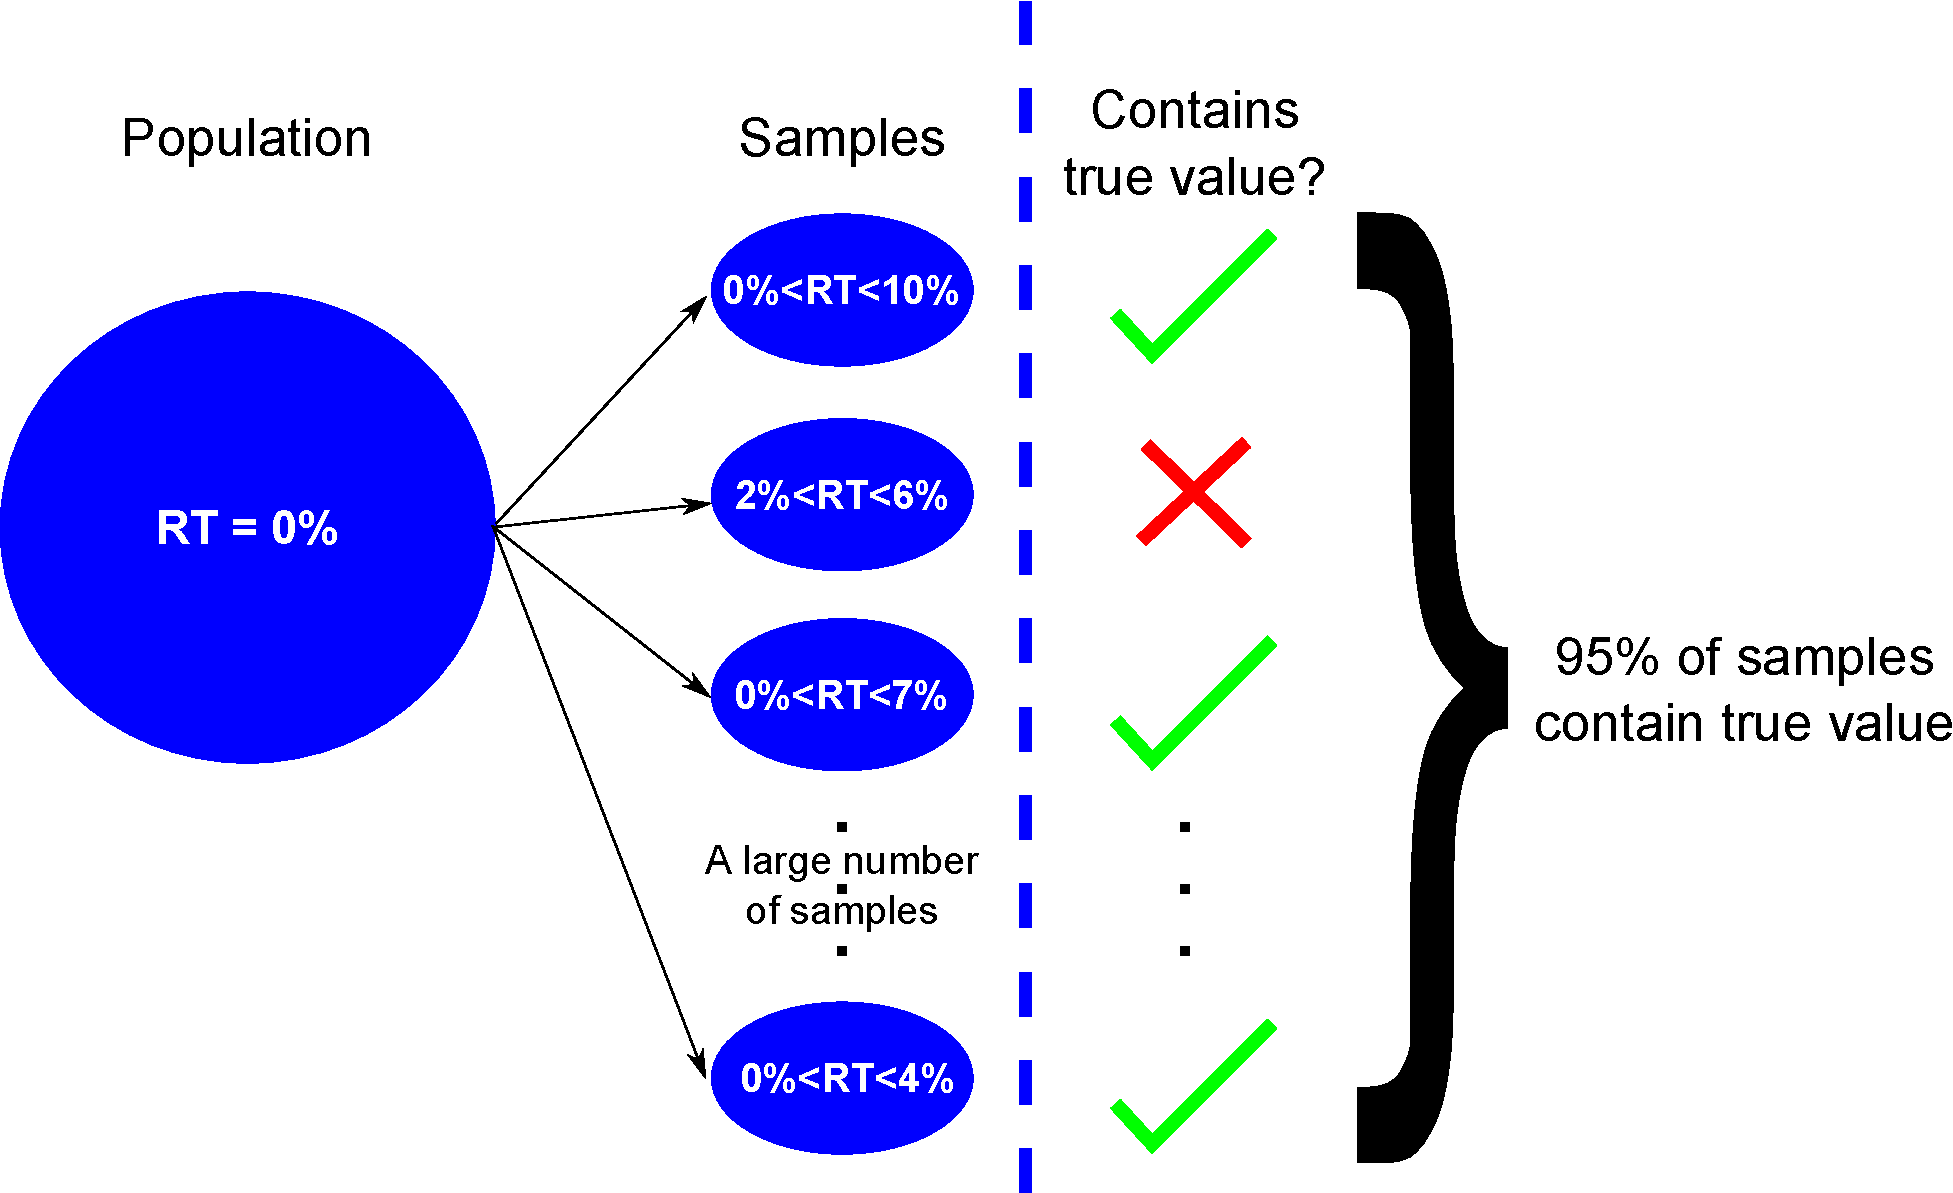
\includegraphics{Posterior_classicalConfidenceInterval.pdf}}
\caption{The classical confidence interval. In each sample, we can calculate a 95\% confidence interval. Across repeated samples from a given population distribution, the classical confidence interval will contain the true parameter value 95\% of time.}\label{fig:Posterior_classicalConfidenceInterval}
\end{figure}

However, what is important to note here is that in reality, we only draw one sample from the population, and we have no way of knowing whether the confidence interval we calculate contains the true parameter value. This means that although 95\% of the time the confidence intervals we calculate will contain the true value of the parameter, and 5\% of confidence intervals will be nonsense! 

In general, a confidence interval represents the uncertainty about the interval we obtained, rather than a statement of probability about the parameter of interest. The uncertainty is quantified in terms of all the samples we \textit{could}
have taken, not only the one we have in our hands.

\subsection{Credible intervals}
Credible intervals, in contrast to confidence intervals, describe our uncertainty in the location of the parameter values and thus can be interpreted as a probabilistic statement about the parameters. They are a Bayesian concept, that is calculated from the posterior density.

In particular, a 95\% credible region satisfies the condition that 95\% of the posterior density's area lies in this parameter range. The statement below,

\textbf{'From our research, we concluded that the percentage of penguins with red tails, $RT$, has a 95\% credible interval of $0\%\leq RT \leq 4\%$.'}

can be interpreted as, 'From our research, we conclude that there is a 95\% probability that the percentage of penguins with red tails, lies in the range $0\%\leq RT \leq 4\%$'.

In general an arbitrary credible interval of $X$\% can be constructed from the posterior density, by finding a region whose area is equal to $\frac{X}{100}$. 

\begin{figure}
\centering
\scalebox{0.35} 
{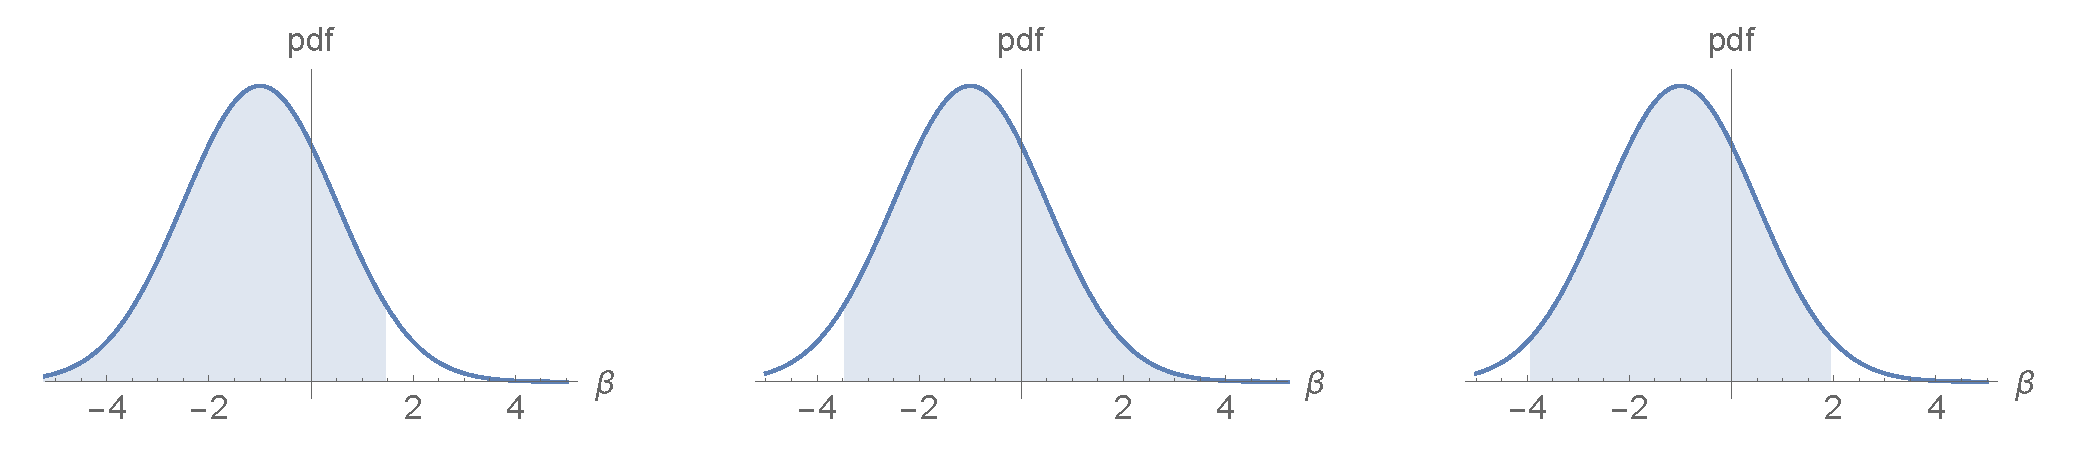
\includegraphics{Posterior_infiniteCredibleIntervals.pdf}}
\caption{Three examples of a 95\% credible interval for the regression parameter $\beta$ of the example described in section \ref{sec:Posterior_parameterUncertainty}.}\label{fig:Posterior_infiniteCredibleIntervals}
\end{figure}

In contrast to the classical confidence interval, a credible interval is more straightforward to understand. It is a probability statement of confidence in the location of a parameter. Also, in contrast to the classical confidence intervals, the uncertainty here refers to our inherent uncertainty in the value of the parameter, rather than counter-factual samples.

There are usually an infinite number of regions which satisfy this condition, as figure \ref{fig:Posterior_infiniteCredibleIntervals} indicates for the regression example used in section \ref{sec:Posterior_parameterUncertainty}. All three of the examples shown in figure \ref{fig:Posterior_infiniteCredibleIntervals} satisfy the condition, that given our choice of model and prior, we conclude that there is a 95\% probability that the parameter lies in this range. 

In order to reduce the number of credible intervals down to one, there are 'industry standards' that are followed in most applied research. We introduce two of the most frequently used metrics now.

\subsubsection{Treasure hunting: The central posterior and highest density intervals}\label{sec:Posterior_CPI}\label{sec:Posterior_HDI}
Imagine you (as a pirate) were told by a fortune-teller that treasure of \$1000 is buried somewhere along the seashore of an imagined island. Further, imagine that the mystic has gone to the trouble of using their past experience, and intuition, to arrive at a posterior density for the location of the treasure, along the x-axis seashore, that is shown in figure \ref{fig:Posterior_CPIvsHDI}. The cost to hire a digger to dig up 1km of coastline is \$100.

Suppose you want to find the gold with 95\% certainty, and maximise your profit in doing so\footnote{This is really a Bayesian Decision Theory question, where you are choosing an \textit{action}, which corresponds to an interval; specifying a constant cost function across the domain.}. In order to reach this level of confidence in plundering the gold, you have the choice of the two 95\% credible intervals shown in figure \ref{fig:Posterior_CPIvsHDI}: the left-hand \textit{central posterior interval}, and the right-hand \textit{highest density interval}.

Both of these intervals have the same area, so we are equally likely to find the gold in either. So which one would be best to choose?

The central posterior interval spans a range of $0.25km-9.75km$ along the beach. This would entail a cost of $9.5\times \$100 = \$950$.

The highest density interval by contrast spans two non-contiguous regions, given by $0km-2.5km$ and $7.5km-10km$. Each has a cost of $2.5\times\$100 = \$250$, meaning a total cost of \$500. We pick the right-hand strategy, and cross our fingers!

Intuitively, we should avoid the left-hand central posterior interval since it this involves digging up more coastline which has a very low probability of containing the gold. The right-hand highest density interval avoids this misspent effort by directing our search efforts towards the areas most likely to contain the treasure.

If it was costly to drive a digger a given distance, without digging, then we might change our minds, and favour the contiguous region of the \textit{central posterior interval} over the \textit{highest density interval}. However, in most practical (non-pirate) situations, the most sensible thing to do is to report the highest density interval.

To work out the upper and lower bounds of an X\% central posterior interval, we find the $\frac{X}{2}\%$ and $(100-\frac{X}{2})\%$ quantiles of the posterior distribution. This will result in an interval that is centred on the median parameter value.

To find the X\% highest posterior interval, we find the set of values which contains this percentage of the posterior density area, with the property that the probability density in this set is never lower than outside.

\begin{figure}
\centering
\scalebox{0.35} 
{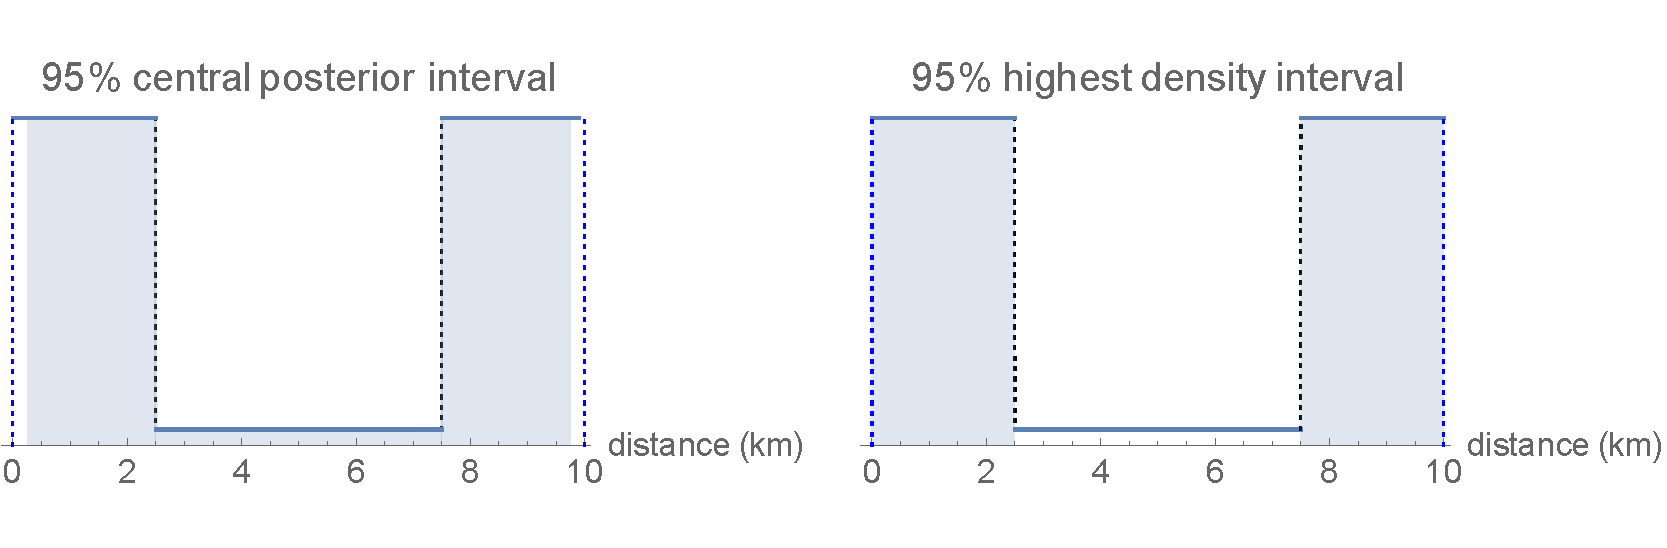
\includegraphics{Posterior_CPIvsHDI.pdf}}
\caption{The posterior probability for treasure being found along the seashore (represented by a linear x-axis).}\label{fig:Posterior_CPIvsHDI}
\end{figure}

For a unimodal, symmetric distribution the central posterior density and highest density intervals will be the same. However, for more complex distributions, this is no longer the case (compare the left and right hand panels of figure \ref{fig:Posterior_CPIvsHDI}).


\subsection{Reconciling the difference between confidence and credible intervals}
It is easy to jump on the bandwagon, and dismiss classical confidence intervals as misleading; favouring the Bayesian alternative definitively. However, in doing so we are somewhat guilty of zealotry\footnote{Fanaticism.}. The two concepts really just represent different measures of uncertainty. As we explained in section \ref{sec:Intro_FrequentistsWorld}, Frequentists view data sets as one of an infinity of exactly repeated experiments, and hence design an interval which contains the true value X\% of the time across all these repetitions. The Frequentist confidence interval states uncertainty in terms of the interval itself. By contrast, Bayesians view the data as fixed, and the parameter as coming from an over-arching distribution. They correspondingly calculate an interval where X\% of the parameter's estimated probability mass lies.

The problem with the classical confidence interval is more that it is often interpreted \textit{incorrectly}, as a \textit{credible} interval. It is not a problem with the concept itself. It just depends on your personal preference, and situation, as to which you find more useful.

The following (slightly silly) example hopefully makes this difference of viewpoint clearer. 

\subsubsection{The interval ENIGMA}
Suppose that at the outbreak of war, you are employed as a code breaker in hut 8 at Bletchley Park. By monitoring enemy communications we are able to identify the \textit{source} of the message, although not its \textit{contents}. The source of the message is either submarine, boat, tank or aircraft. The content of the messages is details of the next domestic target of the enemy, and can either be dams, ports, towns or airfields.

Fortunately, previous code-breakers have managed to decode a significant proportion of messages, and have tallied up the proportions of communications from each source, which resulted in a particular attack destination (see figure \ref{tab:Posterior_confidenceIntervalHistoric}). We also know from experience that the proportion of attacks on each destination are roughly similar.


\begin{table}[htbp]
  \centering
    \begin{tabular}{ccccc}
    \toprule
          & \multicolumn{4}{c}{\textbf{Attack destination}} \\
    \midrule
    \textbf{Communication method} & Dam & Port & Town & Airfield \\
    Submarine & 73\%  & 50\%  & 50\%  & 13\% \\
    Boat  & 9\%   & 25\%  & 25\%  & 16\% \\
    Tank  & 0\%   & 25\%  & 25\%  & 66\% \\
    Aircraft & 18\%   & 0\%  & 0\%   & 5\% \\
    \bottomrule
    Total & 100\% & 100\% & 100\% & 100\% \\
    \end{tabular}%
  \caption{Historical communication frequencies resulting in an attack on a given location.}\label{tab:Posterior_confidenceIntervalHistoric}
\end{table}%

Our job is to predict the next attack destination \textit{given} that we have received the mode of communication used. Since there is uncertainty regarding the attack destination, we shall be making confidence intervals which consist of groups of these entities. We are told to use the most narrow\footnote{We suppose there is a cost to readying a destination against attack.} intervals of width greater than or equal to 75\% in all cases.

From this historical evidence we first put the data into a 'statistics-machine', turning the knob that says 'classical confidence intervals'. The result are the confidence intervals shown in table \ref{tab:Posterior_confidenceIntervalClassical}. In words, this is because the sum of the interval values contained in each column exceeds the threshold. So, for every attack destination, our intervals ensure that the true attack destination lies within the specified sets at least 75\% of the time.

\begin{table}[htbp]
  \centering
    \begin{tabular}{cccccc}
    \toprule
          & \multicolumn{4}{c}{\textbf{Attack destination}} & \multicolumn{1}{c}{\textbf{}} \\
    \midrule
    \textbf{Communications method} & Dam & Port & Town & Airfield   & \textbf{Credibility} \\
    Submarine & \color{red}{$[$73\%}  & \color{red}{50\%}  & \color{red}{50\%$]$}  & 13\%  & \textbf{93\%} \\
    Boat  & \color{red}{$[$9\%}   & \color{red}{25\%}  & \color{red}{25\%}  & \color{red}{16\%$]$}  & \textbf{100\%} \\
    Tank  & 0\%   & 25\%  & 25\%  & \color{red}{$[$66\%$]$}  & \textbf{57\%} \\
    Aircraft & 18\%   & 0\%  & 0\%   & 5\%   & \textbf{0\%} \\
    \bottomrule
    \textbf{Coverage} & \textbf{82\%}  & \textbf{75\%}  & \textbf{75\%}  & \textbf{82\%} &  \\
    \end{tabular}%
  \caption{Classical confidence intervals calculated from data shown in table \ref{tab:Posterior_confidenceIntervalHistoric}. Confidence intervals greater than or equal to 75\% are indicated in red, surrounded by parentheses.}\label{tab:Posterior_confidenceIntervalClassical}%
\end{table}%

We next turn the dial to 'Bayesian credible intervals', and obtain the results shown in table \ref{tab:Posterior_confidenceIntervalBayesian} (see section \ref{sec:Posterior_appendixConfidenceInterval} for a full explanation). In this case, we are implicitly assuming that the choice of destination is a random variable, and that the enemy chooses amongst them uniformly\footnote{Which isn't unreasonable given that we know from experience that the enemy attacks each of these locations in similar proportions.}. In this case, since the sum of interval values in each row exceeds 75\%, we have credible intervals. With these intervals, for each mode of communication, we will ensure that the true attack destination is contained within these destinations at least 75\% of the time.

\begin{table}[htbp]
  \centering
    \begin{tabular}{cccccc}
    \toprule
          & \multicolumn{4}{c}{\textbf{Attack destination}} &  \\
    \midrule
    \textbf{Communication method} & Dam & Port & Town & Airfield   & \textbf{Credibility} \\
    Submarine & \color{red}{$[$73\%}  & \color{red}{50\%}  & \color{red}{50\%$]$}  & 13\%  & \textbf{93}\% \\
    Boat  & \color{red}{$[$9\%}   & \color{red}{25\%}  & \color{red}{25\%$]$}  & 16\%  & \textbf{79}\% \\
    Tank  & 0\%   & 25\%  & 25\%  & \color{red}{$[$66\%$]$}  & \textbf{78}\% \\
    Aircraft & \color{red}{$[$18\%$]$}   & 0\%  & 0\%   & 5\%   &\textbf{78\%} \\
    \bottomrule
    \textbf{Coverage} & \textbf{100\%}  & \textbf{75\%} &\textbf{ 100\%}  & \textbf{66\%}  &  \\
    \end{tabular}%
   \caption{Bayesian credible intervals calculated from data shown in table \ref{tab:Posterior_confidenceIntervalHistoric}. Credible intervals greater than or equal to 75\% are indicated in red, surrounded by parentheses. Note: 'credibility' is calculated by dividing the sum of interval values in each row by the row's total (see section \ref{sec:Posterior_appendixConfidenceInterval} for a full explanation.)}\label{tab:Posterior_confidenceIntervalBayesian}%
\end{table}%

The difference between these two measures is subtle. In fact, as is often the case, the intervals are actually similar, and overlap considerably. But which should we choose? Using the classical confidence intervals, we are assured that whatever destination the enemy chooses, our interval will contain the true attack destination at least 75\% of the time. A Bayesian would criticise the confidence interval for the case of the \textit{Aircraft} communication method, since this is the empty interval! This clearly is nonsensical, since we know that one of the locations is about to be attacked. This error could be particularly costly if attacks coordinated via Aircraft are particularly costly. A Frequentist would argue that since, \textit{at most}, Aircraft communications happen 18\% of the time (for dams), this isn't something to worry about.

A Bayesian would also criticise a classical confidence interval, since for a given communication mode, what is the use in worrying about all the other communication modes? We aren't uncertain about the communication mode!

A Frequentist would argue that for attacks on airfields, the Bayesian confidence intervals only correctly predict this as the attack destination 66\% of the time. Again, if these types of attack are particularly costly, then this interval might not be ideal\footnote{If we were to assign costs to each of these attack events, then we could work out optimal intervals, although this is the realm of Bayesian Decision Theory; not covered in this text.}. A Bayesian would argue that, assuming a uniform prior, this type of attack only happens 25\% of the time, and so is not something to worry about. Further, for every mode of communication, our credible intervals are guaranteed to never be nonsense, in contrast to the classical confidence interval.

\section{Point parameter estimates}
Whilst it is beneficial to estimate the entire posterior distribution for a particular parameter, we are often required to give point estimates. This is sometimes for direct comparison with Frequentist approaches, but more often it is to allow people not versed in Bayesian statistics to make decisions\footnote{The correct process in order to make decisions using posterior distributions is through decision theory, not covered in this text. A good review of this field is provided in \cite{robert2007bayesian}.}. We want to reiterate, that we are \textit{not} advocating these estimators\footnote{Rules that take an input, and produce estimates.} as a replacement to providing the entire posterior distribution; only that they are useful summaries which supplement an analysis.

There are three main approaches here, although we argue that only two out of the three should be used. These estimators can be summarised as:

\begin{itemize}
\item The posterior mean.
\item The posterior median.
\item The maximum a posteriori estimator (MAP).
\end{itemize}

The posterior mean is simply defined for a univariate-continuous example as:

\begin{equation}
\mathrm{E}[\theta|data] = \int\limits_{\Theta} \theta p(\theta|data)\mathrm{d}\theta
\end{equation}

For the discrete case, we replace the integrals above with summations (see section \ref{sec:Probability_meanVariance}). 

The posterior median is the point of a posterior distribution to which 50\% of its area (the probability), lies to its left. The MAP estimator is simply the highest point in the posterior (see figure \ref{fig:Posterior_meanMedianMAP}).

Whilst each of these three estimators can be optimal for a given loss function\footnote{A decision theoretic concept, again.}, we believe that there is a clear hierarchy of these estimators. At the top of the hierarchy - denoting our preferred estimator - we have the posterior mean. This is our favourite for two reasons: firstly, it normally yields \textit{sensible} estimates, which are fairly representative of the central position of the posterior distribution; secondly, and more mathematically, this estimator makes sense from a measure-theoretic perspective, since the quantity of interest is a probability not a density. The density depends on the particular parameterisation that we choose, the probability should not. Don't worry about this last point too much, we just wanted to mention it for completeness. Next down the hierarchy we have the posterior median. This is usually pretty close to the mean (see figure \ref{fig:Posterior_meanMedianMAP}), and is often indicative of our posterior distribution. It is sometimes preferable to use a median if the mean is heavily-skewed by a slowly-changing density, although the choice between the two estimators depends on circumstance.

At the bottom of the hierarchy, we have the MAP estimator. Proponents argue that the simplicity of this estimator is a benefit. Since it maximises the posterior, across values of the parameter, we do not actually need to calculate the tricky denominator (see chapter \ref{chap:denominator}), as this is independent of the parameter. This means that it is often feasible to find the MAP estimator exactly, even if this is not possible for the other two measures. However, its simplicity is misleading. Importantly, the mode of a distribution often lies away from the majority of the probability distribution's area, and is hence not a particularly indicative central measure of the posterior. Secondly, and mathematically, this estimator does not make sense because it relies on the density, which depends on the particular parameterisation in question.

The bottom line is that one should not use the MAP estimator unless you have a \textit{very} good reason for doing so. 

\begin{figure}
\centering
\scalebox{0.4} 
{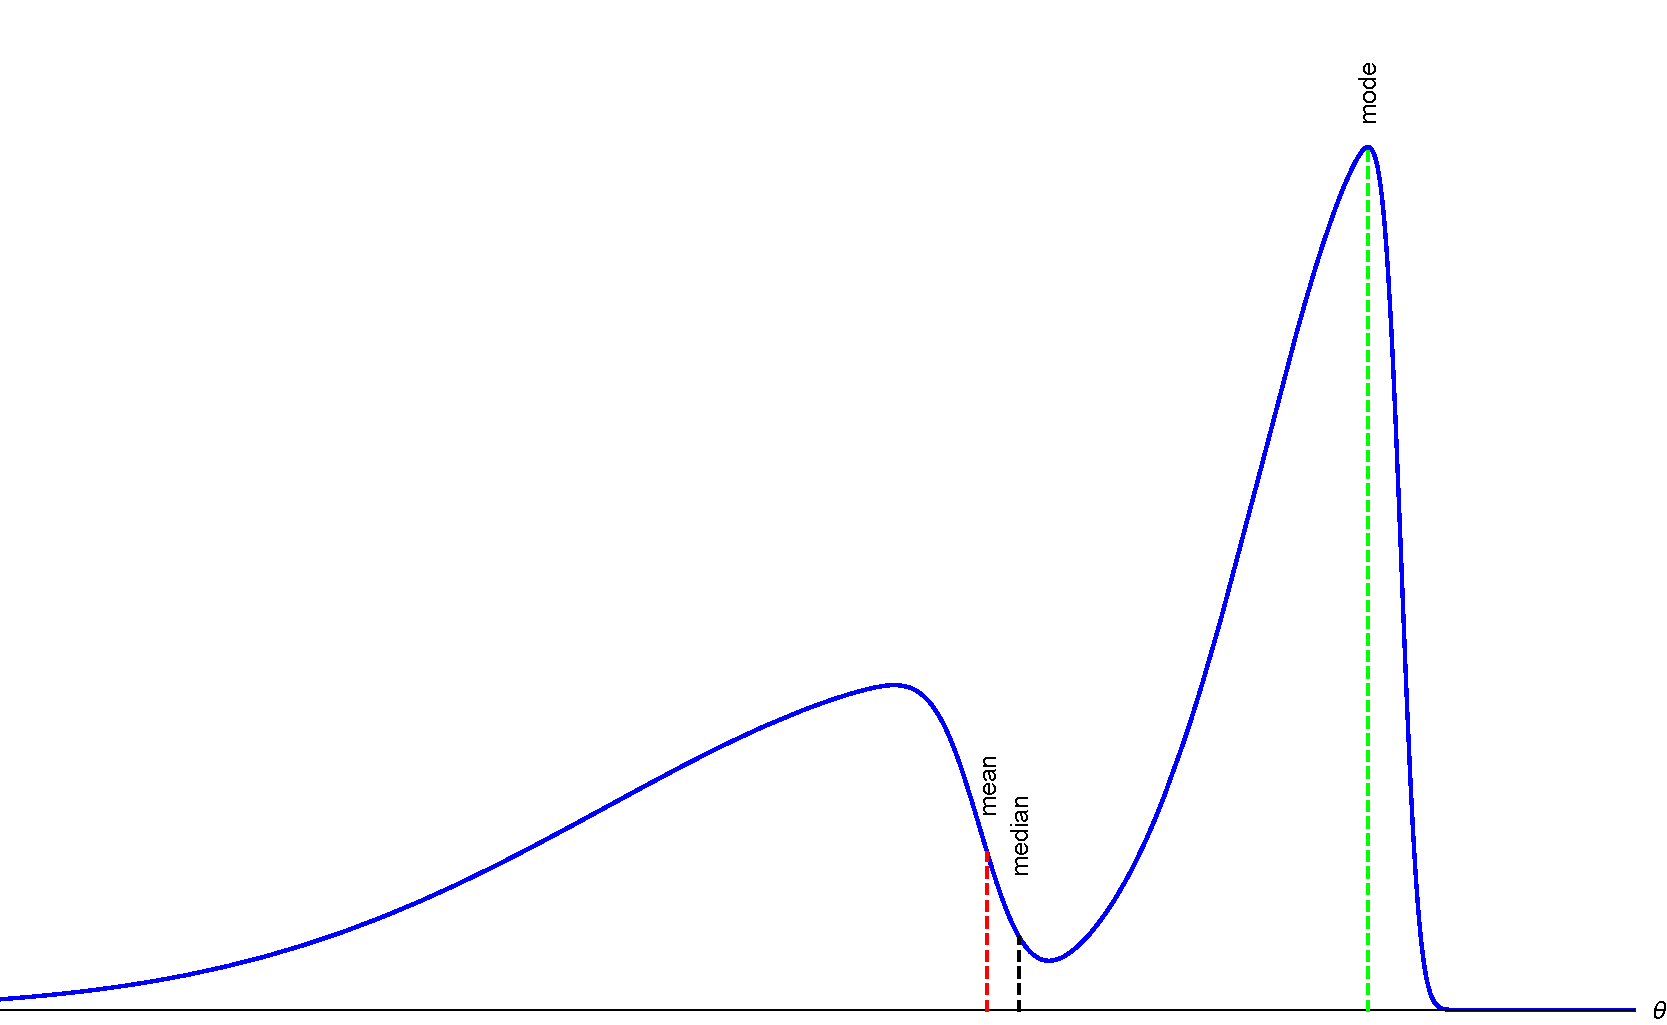
\includegraphics{Posterior_meanMedianMAP.pdf}}
\caption{The mean, median and mode for a skewed, multi-modal distribution.}\label{fig:Posterior_meanMedianMAP}
\end{figure}


\section{Prediction using predictive distributions}
Parameters of a statistical distribution are typically only of interest insomuch as they influence \textit{real variables}, for which we collected data in the first place. Be it income levels, disease cases, or electoral votes; the data is what drove us to conduct a statistical analysis. As such, it is frequently useful to compare models (which may have very different statistical formulations) using this common currency, of \textit{data}.

Before we have run our model, we only have our prior views of the likely values of parameters. It is often informative to convert from the currency of \textit{parameters}, to that of \textit{data}, in order to evaluate the tangible implications of the chosen priors\footnote{See chapter \ref{chap:Prior} for a much more in-detail discussion.}.

Also, after we have fed our priors and likelihoods into the Bayesian formula, we are outputted with the posterior distribution for our parameters of interest. Fortunately, both of these are simple, due to the manipulable nature of probabilities.

\subsection{Example: number of Republican voters within a sample}
You find yourself working for a polling organisation, ahead of the next US Presidential election. Your job is to try to predict, out of a sample of 100 people, what will be the number voting for the Republican party. Based on previous work, you expect that the proportion of Republican voters in a sample, $\theta$, can be represented by the prior distribution, $p(\theta)$, shown in the top-left of figure \ref{fig:Posterior_priorPosteriorPredictiveVoting}. To evaluate the implications of this prior, we would like to know what this means in terms of number, $x$, of people out of our sample of 100, who will vote for the Republicans; in other words, the \textit{prior predictive distribution}. Fortunately, we can obtain this by manipulating probabilities, although we need to specify a likelihood function, $p(x|theta)$; in this case we pick a binomial distribution\footnote{The relevance and nice fit of this distribution is explained in full in chapter \ref{chap:Likelihoods}, so do not worry if you don't follow its use here.}. The prior predictive distribution here is essentially the marginal distribution of $x$, which we know from section \ref{sec:Probability_marginal} can be obtained by integrating\footnote{Since the parameter is continuous here.} out the dependence of the parameter $\theta$ from the joint distribution $p(x,\theta)$:

\begin{equation}\label{eq:Posterior_priorPredictiveVoting}
\begin{align}
p(x) &= \int\limits_{0}^{1} p(x,\theta) \mathrm{d}\theta\\
&= \int\limits_{0}^{1} p(x|\theta) p(\theta) \mathrm{d}\theta
\end{align}
\end{equation}

\begin{figure}
\centering
\scalebox{0.4} 
{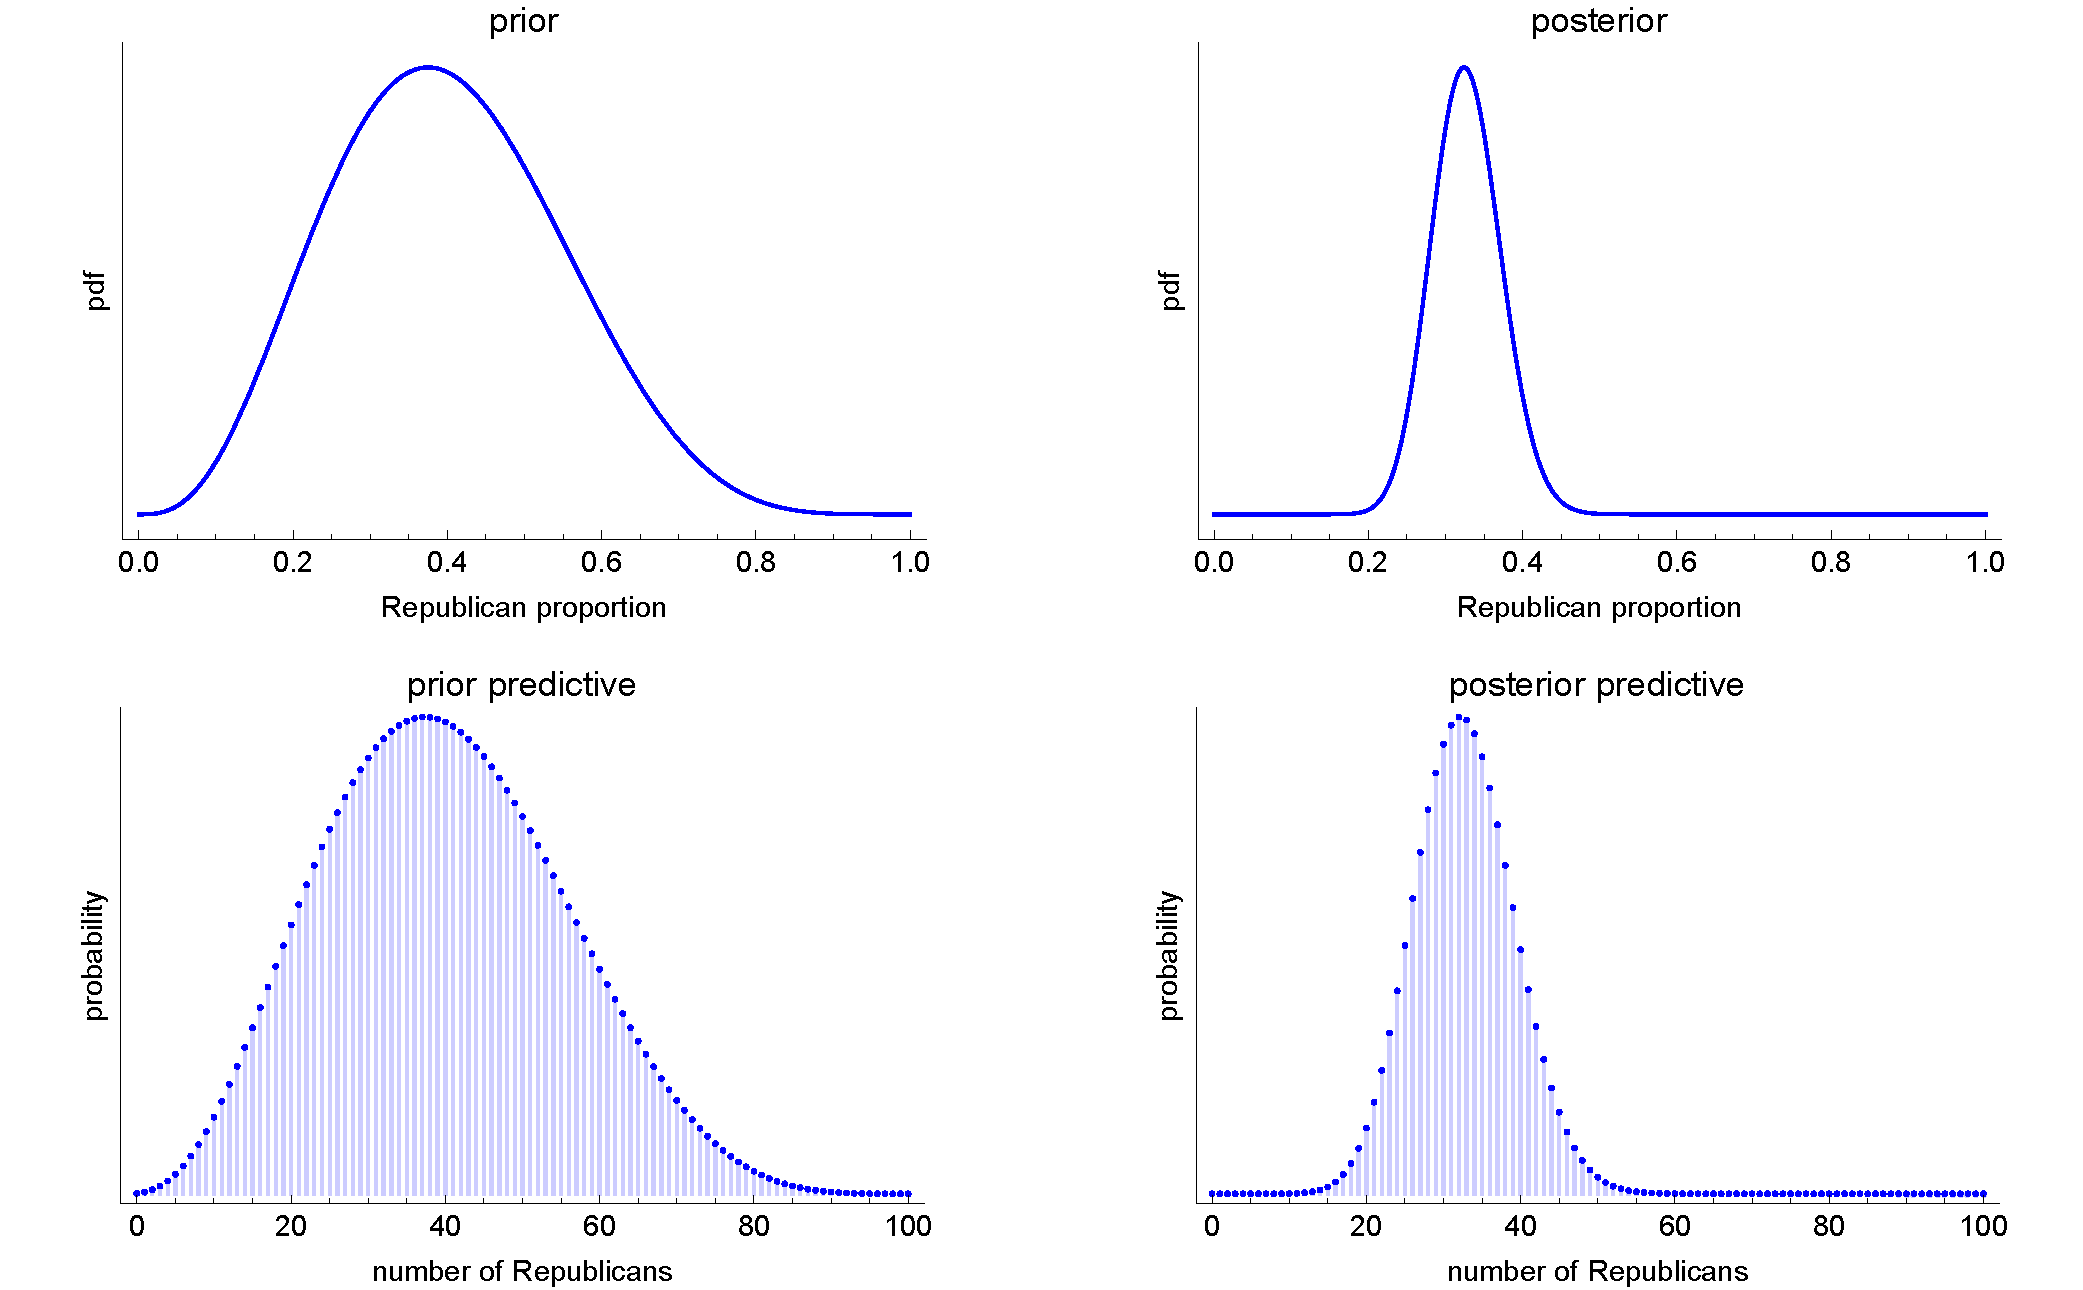
\includegraphics{Posterior_priorPosteriorPredictiveVoting.pdf}}
\caption{Top-left: the prior proportion of people voting for the Republican party in a sample of 100, resulting in the prior predictive distribution shown in the bottom-left. Top-right: the posterior proportion of people voting Republican, resulting the bottom-right posterior predictive distribution.}\label{fig:Posterior_priorPosteriorPredictiveVoting}
\end{figure}


where to get to the second line from the first, we have used the conditional law of probability (\ref{eq:Probability_conditionalProbability}), to decompose the joint distribution into a conditional and prior. Notice that the prior predictive distribution is essentially a sum of the probability of $x$ conditional on $\theta$, weighted by our prior probability to that proportion, $\theta$, voting Republican. this case, this results in the intuitive result, where the prior density and the prior predictive distribution\footnote{This is predictably called a Beta-binomial distribution, since it is made from combining a Beta prior, with a Binomial likelihood. Don't worry though, we will discuss this in detail in chapter \ref{chap:conjugate}.} exactly line up (albeit on different scales).

After our first sample of 100 people from that particular location, we find that 32 of them would vote Republican. We use this data to calculate our likelihood, then combine this with our prior via Bayes' rule; obtaining the posterior density shown in the top-right of figure \ref{fig:Posterior_priorPosteriorPredictiveVoting}. Our job is now to estimate the number of people who will vote republican in a new sample, of the same size. Ideally, we would like to have a probability distribution to describe all the possible outcomes. This distribution is known as the \textit{posterior predictive distribution}, because it is that which we would predict \textit{after} obtaining our data sample. It is written as $p(x'|x)$ where $x'$ represents the number of people voting Republican in the new sample, and $x$ is the number voting Republicans in the previous sample ($x=32$). We can use a method exactly analogous to that which we used previously, by integrating out $\theta$ dependence of the joint distribution of $x'$ and $\theta$, although now we have to condition on $x$:

\begin{equation}\label{eq:Posterior_posteriorPredictiveVoting}
\begin{align}
p(x'|x) &= \int\limits_{0}^{1} p(x',\theta|x) \mathrm{d}\theta\\
&= \int\limits_{0}^{1} p(x'|\theta,x) p(\theta|x) \mathrm{d}\theta\\
&= \int\limits_{0}^{1} p(x'|\theta) p(\theta|x) \mathrm{d}\theta
\end{align}
\end{equation}

Note that to get from the second line from the first, we have used the same conditional probability law  (\ref{eq:Probability_conditionalProbability}), as we used for the prior predictive case. The only difference here is that we are additionally conditioning on $x$. To get from the second to the third line we have used a typical assumption, which is that once $\theta$ is known, the likelihood for our new sample does not depend on the previous data $x$. Another way to think about this is that all the information in $x$ has been used to estimate $\theta$; meaning that it does not confer any further information which is helpful for predicting $x'$. Again, we note in figure \ref{fig:Posterior_priorPosteriorPredictiveVoting} how the posterior predictive distribution lines up exactly with the posterior distribution of $\theta$. This makes intuitive sense, since if we predict the most likely \textit{proportion} to vote Republicans is 0.32, we should expect that this will translate into the most likely \textit{number} of $0.32\times 100=32$, in a sample of 100.

\subsection{Example: interest rate hedging}
Suppose that you work as an analyst in an investment bank, focussing on predicting the actions of the central bank, so that your investments can be sufficiently hedged. The return of a certain investment, $x$, is probabilistically dictated by the rate of interest, and is also discrete; following a poisson distribution with rate parameter given by the chosen rate. Imagine that the current rate of interest is 1\%, and the bank sets rates at 0.5\% intervals; yielding a discrete distribution of possible values: $i\in[0.5\%, 1.0\%, 1.5\%, 2.0\%, 2.5\%,3.0\% ]$; resulting in the likelihood\footnote{Do not worry about the use of likelihoods here, as we shall explain this concept fully in chapter \ref{chap:Likelihoods}.} shown in figure \ref{fig:Posterior_likelihoodInterestRate}.

\begin{figure}
\centering
\scalebox{0.65} 
{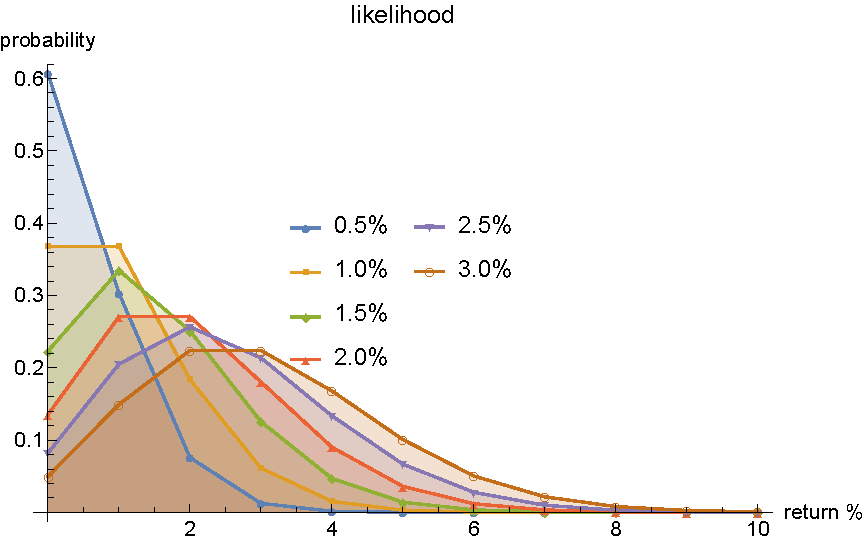
\includegraphics{Posterior_likelihoodInterestRate.pdf}}
\caption{The likelihood of different rates of return across different central bank interest rates.}\label{fig:Posterior_likelihoodInterestRate}
\end{figure}

The pre-data-analysis probabilities that your in-house economist gives to each different central bank rate are shown in figure \ref{fig:Posterior_priorPosteriorInterestRate}. After combining these expert views with a probabilistic model, which looks at historical rate decisions, this results in the posterior distribution of probabilities shown in figure \ref{fig:Posterior_priorPosteriorInterestRate}; illustrating considerable discordance between the data's view, and those of your economist\footnote{This might indicate that your economist doesn't know his head from his hands, \textit{or} he believes there is reason to suggest that this rate decision will be different to those historically.}.

\begin{figure}
\centering
\scalebox{0.45} 
{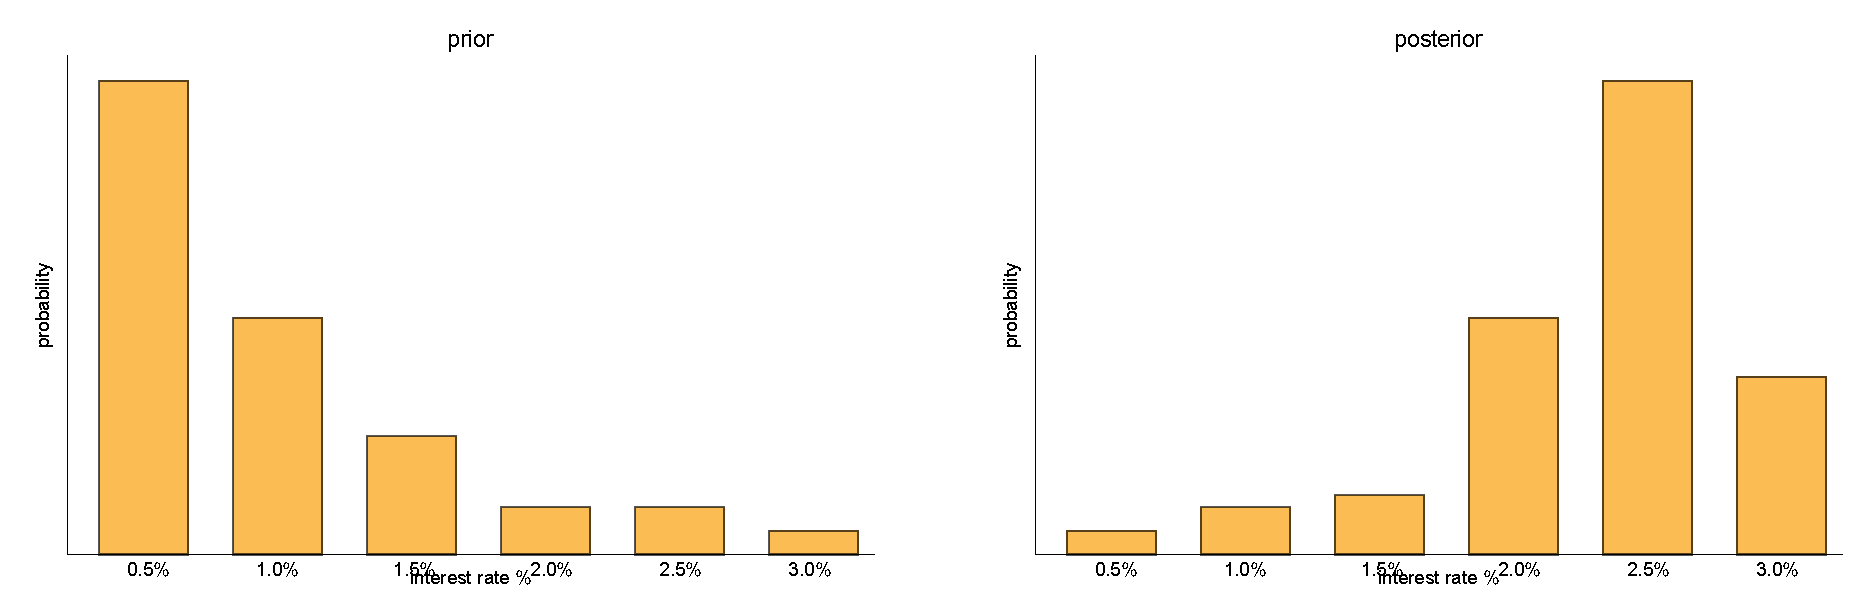
\includegraphics{Posterior_priorPosteriorInterestRate.pdf}}
\caption{The prior and posterior probabilities of different central ban interest rates.}\label{fig:Posterior_priorPosteriorInterestRate}
\end{figure}

From the prior distribution, $p(i)$, we would like to estimate the probability of particular rates of investment return. Mathematically, what we want is the marginal distribution of investment return, $p(x)$. Fortunately, we know from section \ref{sec:Probability_marginal}, that we can get a marginal distribution from a joint distribution by summing (for a discrete parameter) across values of the parameter:

\begin{equation}\label{eq:Posterior_InterestpriorPredictiveDistribution}
\begin{align}
p(x) &= \sum\limits_{i=0.5\%}^{3.0\%} p(x,i)\\
&= \sum\limits_{i=0.5\%}^{3.0\%} p(x|i) p(i)
\end{align}
\end{equation}

This distribution essentially weights each of the conditional probabilities, $p(x|i)$, by its corresponding prior probability $p(i)$ (see the left-hand side of figure \ref{fig:Posterior_priorBuildInterestRate}), then sums them to yield the marginal probability of the data (see the right hand side of figure \ref{fig:Posterior_priorBuildInterestRate}).

\begin{figure}
\centering
\scalebox{0.4} 
{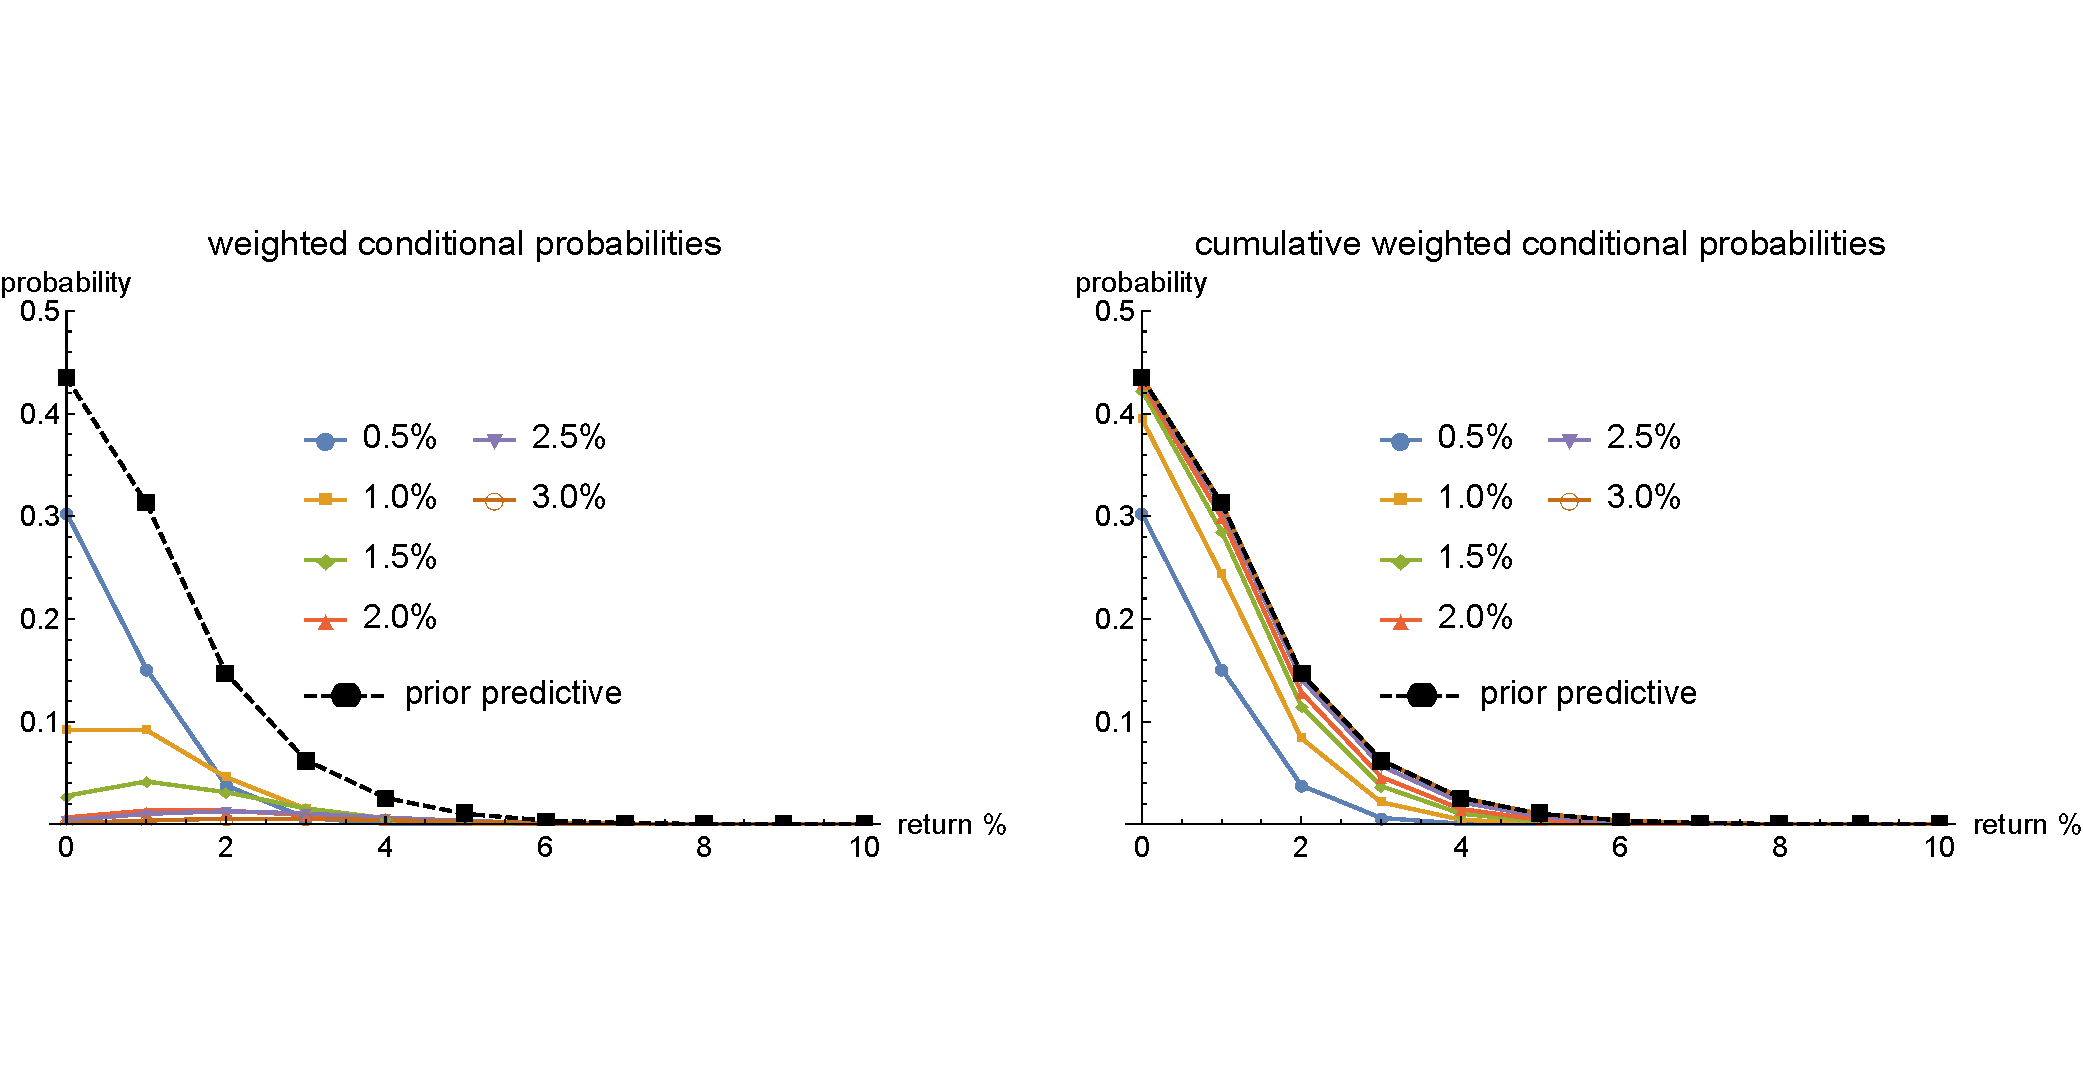
\includegraphics{Posterior_priorBuildInterestRate.pdf}}
\caption{Building the prior predictive distribution, as a sum of weighted conditional probabilities. Left: the weighted conditional probabilities (compare with figure \ref{fig:Posterior_likelihoodInterestRate}). Right: the cumulative weighted conditional probabilities, which converge on the prior predictive distribution.}\label{fig:Posterior_priorBuildInterestRate}
\end{figure}

To calculate the posterior predictive distribution, we proceed in an analogous way to the prior case. What we would like to obtain is $p(x'|x)$, where $x'$ indicates the predicted return on the investment, and $x$ represents the historical data that has been used to produce the posterior. We can again achieve this by summing out all $i$ dependence from the joint-conditional distribution $p(x',i|x)$:

\begin{equation}
\begin{align}
p(x'|x) &= \sum\limits_{i=0.5\%}^{3.0\%} p(x',i|x)\\
&= \sum\limits_{i=0.5\%}^{3.0\%} p(x'|i,x) p(i|x)\\
&= \sum\limits_{i=0.5\%}^{3.0\%} p(x'|i) p(i|x)
\end{align}
\end{equation}

Note that we have gone from the second line to the third line, because we suppose that, once $i$ is known, the likelihood is independent of past values of $x$, and thus $p(x'|i,x)=p(x'|i)$. Also, note the similarity between this derivation and that for the prior predictive distribution in \ref{eq:Posterior_InterestpriorPredictiveDistribution}; the only difference in both second lines, is that in the posterior case, everything is conditioned on the historical values of $x$. We suppose that the likelihood function remains constant, so that like the prior predictive distribution, the posterior predictive distribution is obtained by weighting each of the conditional probability lines $p(x'|i)$ by a probability - in this case, the posterior probability for that value of $i$. 

The resultant prior and posterior distributions are shown in figure \ref{fig:Posterior_priorPosteriorPredictiveInterestRate}. We notice that the posterior predictive distribution is shifted rightwards, towards higher investment returns, because of the fact that the posterior expected interest rate is higher than for the prior case.

\begin{figure}
\centering
\scalebox{0.65} 
{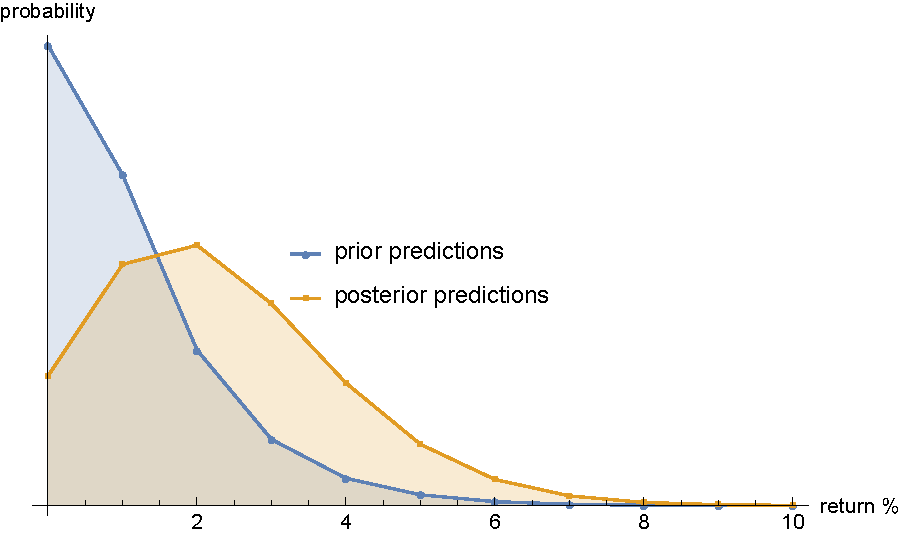
\includegraphics{Posterior_priorPosteriorPredictiveInterestRate.pdf}}
\caption{The prior and posterior predictive distributions for investment returns.}\label{fig:Posterior_priorPosteriorPredictiveInterestRate}
\end{figure}

\section{Model comparison using the posterior}
Suppose we have two competing models ($M1$ and $M2$) which we could use to explain a given dataset, and would like a way of evaluating their respective worth. The Bayesian framework can be used to incorporate the choice between two (or more) models, in a straightforward way. Suppose we denote a discrete parameter, $M\in[M1,M2]$, which indexes the choice of model. A way of gauging a model's performance is to calculate the probability of the model \textit{given} the data obtained, $p(M|data)$. Since we have introduced this new parameter $M$, we can use Bayes' rule to calculate this quantity:

\begin{equation}\label{eq:Posterior_modelGivenDataProbability}
p(M|data) = \frac{p(data|M) p(M)}{p(data)}
\end{equation}

Looking at (\ref{eq:Posterior_modelGivenDataProbability}) in detail, we examine the following quantities: $p(data|M)$, which represents what we, in the single model set-up, simply call $p(data)$; the $p(M)$ which represents our \textit{a priori} probability of each model being correct; and $p(data)$, which in this case represents the marginal probability of the model when we have summed out our dependence on the model choice:

\begin{equation}
\begin{align}
p(data) &= \sum\limits_{M=M1}^{M2} p(data,M)\\
&= \sum\limits_{M=M1}^{M2} p(data|M) p(M)\\
&= p(data|M1) p(M1) + p(data|M2) p(M2)
\end{align}
\end{equation}

We can then calculate the ratio of the probabilities of each model, given the data obtained:

\begin{equation}\label{eq:Posterior_modelComparisonFull}
\begin{align}
\frac{p(M1|data)}{p(M2|data)} &= \frac{p(data|M1) p(M1)}{p(data|M2) p(M2)}\\
&= \frac{p(data|M1)}{p(data|M1)} \times \frac{p(M1)}{p(M2)}\\
&= BF \times \frac{p(M1)}{p(M2)}
\end{align}
\end{equation}

If this ratio is greater than 1, then this test suggests that we should favour model 1, and vice versa if the ratio is less than 1. We have also defined a quantity, $BF$, called the \textit{Bayes Factor}:

\begin{equation}\label{eq:Posterior_bayesFactorDefinition}
BF = \frac{p(data|M1)}{p(data|M1)}
\end{equation}

This factor represents in a narrow sense, the strength of support of model 1, over model 2, provided by the data. Note that if our prior probabilities of each model are identical, $p(M1) = p(M2) = \frac{1}{2}$, then:

\begin{equation}
\frac{p(M1|data)}{p(M2|data)} = BF
\end{equation}

And the choice of model is determined solely through the Bayes Factor. 

However, there is uncertainty over when is the BF enough to prefer one model over another. Whereas a BF of 100 may be enough to prefer a given model, how about 1.01? Jeffrey's scale (introduced in chapter \ref{chap:ModelFit}), is an arbitrary, albeit industry-standard, meter to determine when a given model should be preferred over another.

I do importantly want to state here, that this is \textit{not} the correct way to choose between competing models. We will learn a much more nuanced, and reasonable way of choosing between models when we introduce the concept of \textit{Posterior Predictive Checks} in chapter \ref{chap:ModelFit}. That is not to say that these methods introduced above can't be used as additional evidence for or against a given model, it is just that they should not be used as \textit{sole}, or even \textit{primary}, method.

\subsection{Example: epidemiologist comparison}
Suppose you find yourself in the (bizarre) situation, where you would like to compare two epidemiologists in terms of their ability to predict the underlying proportion of individuals having colds. The first epidemiologist, named \textit{optimist}, gives his estimation of the proportion of individuals with colds, $\theta$, via the (prior) distribution shown in figure \ref{fig:Posterior_bayesFactorFluEpidemiologist}. The second, named \textit{pessimist}, gives a slightly more conservative estimate of the underlying proportion of individuals with colds (also shown in figure \ref{fig:Posterior_bayesFactorFluEpidemiologist})\footnote{Here I have actually generated these priors by assuming, for the optimist, $\theta\sim Beta[3,40]$ and $\theta\sim Beta[4,15]$ for the optimist and pessimist respectively.}.

The data we have is 10 samples of 100 people, where survey respondents have indicated whether or not they are currently suffering from a cold, $\boldsymbol{x} = \{22, 18, 18, 12, 16, 15, 21, 19, 14, 15\}$. 

We can then go through and calculate the $p(data|M)$ for each of the two different priors (see figure \ref{fig:Posterior_bayesFactorFluEpidemiologist} for a graphical depiction of this), by simply integrating the joint density with respect to $\theta$:

\begin{equation}
\begin{align}
p(data) &= \int\limits_{0}^{1} p(data,\theta) \mathrm{d}\theta\\
&= \int\limits_{0}^{1} p(data|\theta) p(\theta) \mathrm{d}\theta
\end{align}
\end{equation}

where $p(data|\theta)$ is the likelihood function\footnote{Which here is taken to be a binomial density.}. Carrying out this integrand for each of the different priors results in the probabilities of data given in the bottom panel of figure \ref{fig:Posterior_bayesFactorFluEpidemiologist}. From this, we note two things: firstly both of the probabilities are very small. This is typical, and is unsurprising when you consider the vast array of possible outcomes that could have occurred. Secondly, we see that the probability of the data for the pessimist is higher than for the optimist. Indeed, we can calculate the Bayes factor via (\ref{eq:Posterior_bayesFactorDefinition}), and find here $BF \approx 6$ for the pessimist vs the optimist model; which, if we assign equal priors to each model, results in us favouring the pessimistic perspective.

I should add that this use of Bayes factors is atypical; it is not usually used as a means of testing between differing priors. However, since this forms part of a model, we can test its support with the data like any other part.

\begin{figure}
\centering
\scalebox{0.45} 
{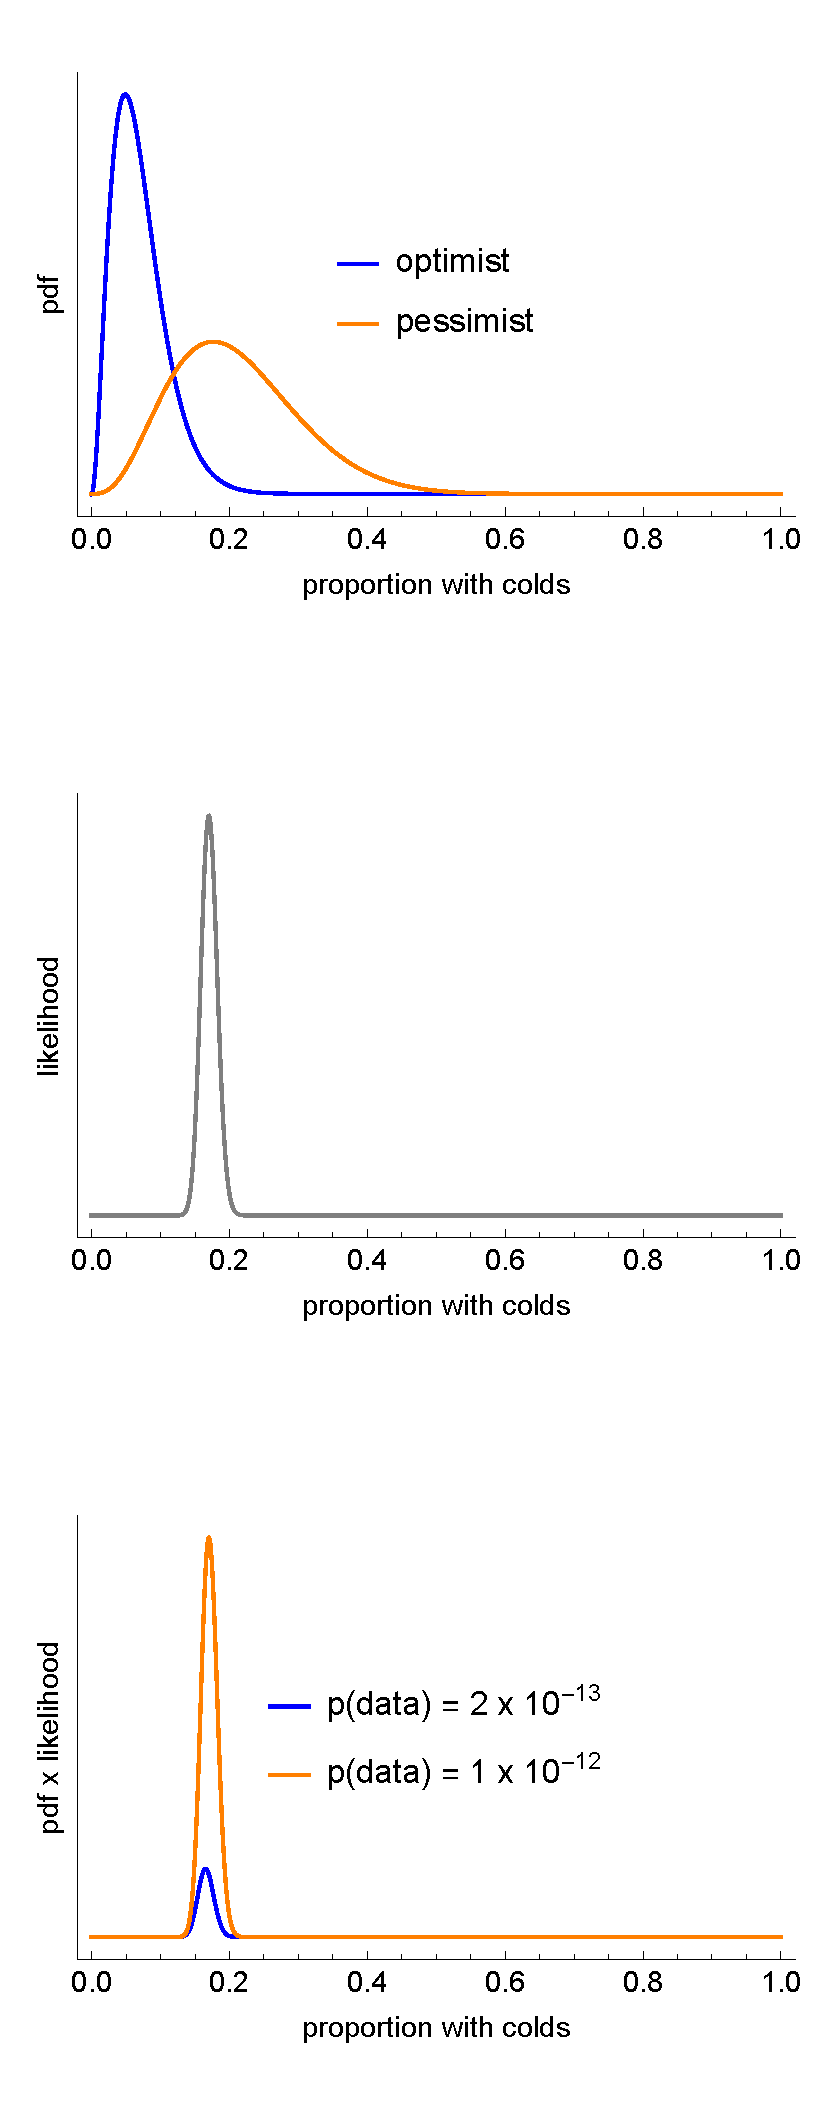
\includegraphics{Posterior_bayesFactorFluEpidemiologist.pdf}}
\caption{Calculating the probability of the data for the two epidemiologists' opinions on colds.}\label{fig:Posterior_bayesFactorFluEpidemiologist}
\end{figure}

\subsection{Example: customer footfall}
Suppose that your job at a consultancy is to try to develop a statistical model which describes the footfall of customers into a particular store location at 1pm-2pm, over a span of 2 months. We have collected the data shown in the histogram in the left hand panel of figure \ref{fig:Posterior_modelComparisonFootfall}. 

Firstly, we fit a poisson likelihood to the data, since we know that the data were collected over a fixed period of time, and we might initially posit that the entry of an individual into the store is independent of others' entry\footnote{See chapter \ref{chap:distributions} for a more complete examination of this distribution.}. However, we notice the point to the far right of the histogram. A poisson distribution is not reasonably able to cope with this degree of extremity, since it has a variance which is given by its mean - in this case this is estimated to be 10.5. For a small dataset, it seems hard to believe that a data point at 26, could have been generated from such a model\footnote{This would be more easily seen by posterior predictive checks.}.

An alternative model, which allows for a variance which exceeds its mean is the negative binomial. This choice of distribution would make most sense if we believed that one consumers' entry into a store was not independent of another's. This would make sense if people tend to shop in groups, and if the shop is outside, with people tending to enter \textit{en masse} when it rains. The expense of this extra freedom, compared to the poisson, is that it is a two-parameter distribution, opposed to a single one.

Again, we can go through and calculate the probability of the data in each case (see figure \ref{fig:Posterior_modelComparisonFootfall}), and then take the ratio to find $BF\approx 3$ for the negative binomial vs the poisson, which is unsurprising given the extreme observation. Here though, we might be tempted to \textit{a priori} favour the poisson, due to its relative parsimony; setting a prior for this model that more than accounted for its loss in explanatory power. This might mean that overall we end up using the poisson model, acknowledging its shortcomings in predicting extreme footfall. However this depends on the nature of these extreme events. If they account for a disproportionate part of sales, then it may be worth the extra flexibility of the negative binomial. If by contrast, the extreme footfall is often due to rain, where consumers simply enter to avoid getting wet, and fail to buy, we would perhaps not be so worried about the modelling of these events.

\begin{figure}
\centering
\scalebox{0.45} 
{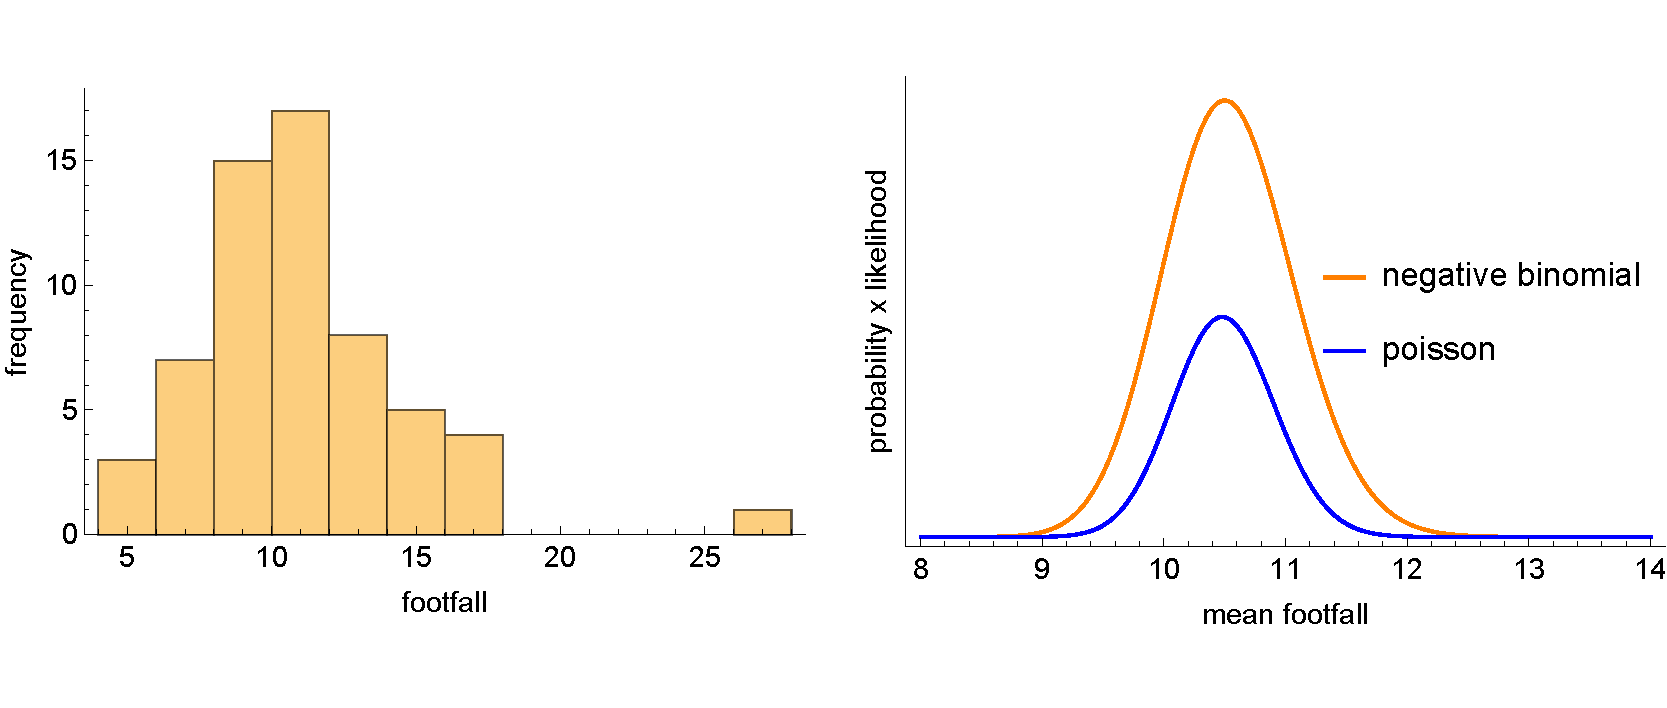
\includegraphics{Posterior_modelComparisonFootfall.pdf}}
\caption{Left: the footfall data. Right: the area under the curves represents the probability of the data from each of the two models.}\label{fig:Posterior_modelComparisonFootfall}
\end{figure}



\section{Model comparison through posterior predictive checks}
The posterior is also the predominant means for testing the worth of a model, and comparing different models. The idea behind this method is that a reasonable model should be able to \textit{simulate} data which is in some correspondence with the \textit{real} data. 

The idea behind this methodology is to simulate data, of the same dimension, and in the case of regression, with the same covariates, then compare this to the actual data. To go about simulating the data, we typically go through the following two steps:

\begin{enumerate}
\item Sample parameter values from the posterior: $\theta\sim p(\theta|x)$
\item Use these parameters in the likelihood function, then use this distribution to sample new data: $x'\sim p(x'|\theta)$
\end{enumerate}

We shall see a full description of this methodology in chapter \ref{chap:ModelFit}, so I only mention it briefly as a sign of things to come, and illustrate its basic mechanism through the following example.

\subsection{Example: stock returns}
Suppose we are tasked with modelling the daily-stock returns for a particular company over a one year period (see the leftmost panel of figure \ref{fig:Posterior_PPCstockReturns}). 

We firstly notice the symmetry of the returns, and reason that a normal likelihood may be a reasonable fit. We then use Bayes' rule, with appropriate priors (see chapter \ref{chap:conjugate} for a good guide as to appropriate priors for the parameters of a normal distribution), to calculate posteriors for the mean and variance of this distribution. We then use these posterior distributions, which are fairly narrow, to firstly sample the mean, and variance, then use a normal likelihood to simulate a number of samples of the same size as the original data. For each of the simulated series, we compare the histogram of returns to that of the actual dataset. A typical plot of this form is shown in the middle panel of figure \ref{fig:Posterior_PPCstockReturns}. We notice that the simulated data is a poor fit to the actual in a number of ways: it under-predicts the number of days with little stock movement; there are an over-abundance of days with moderate returns; and an under-weighting given to those days with more extreme stock movements. Overall, the dataset is not well represented by our model.

Instead of throwing in the towel, we decide to go for a distribution with fatter tails, which allows a greater degree of flexibility than that of a normal - a student's t distribution. We then go through the rigmarole of setting priors on its three parameters, and finally use Bayes' rule to find the posteriors of these. We then use the posterior distributions to sample these parameters, and then a t-likelihood to simulate the data a number of times. What we now typically see is a better fit (see the rightmost panel of figure \ref{fig:Posterior_PPCstockReturns}), with a similar abundance of observations near zero, and a similar distribution of extreme daily movements.

Whilst these visual checks may become cumbersome with more complex data series, it is always a good idea to at least start with them, since the eyes can often be less misleading that, for example, p-values. However, we postpone a more complete discussion of posterior predictive checks until chapter \ref{chap:ModelFit}.

\begin{figure}
\centering
\scalebox{0.35} 
{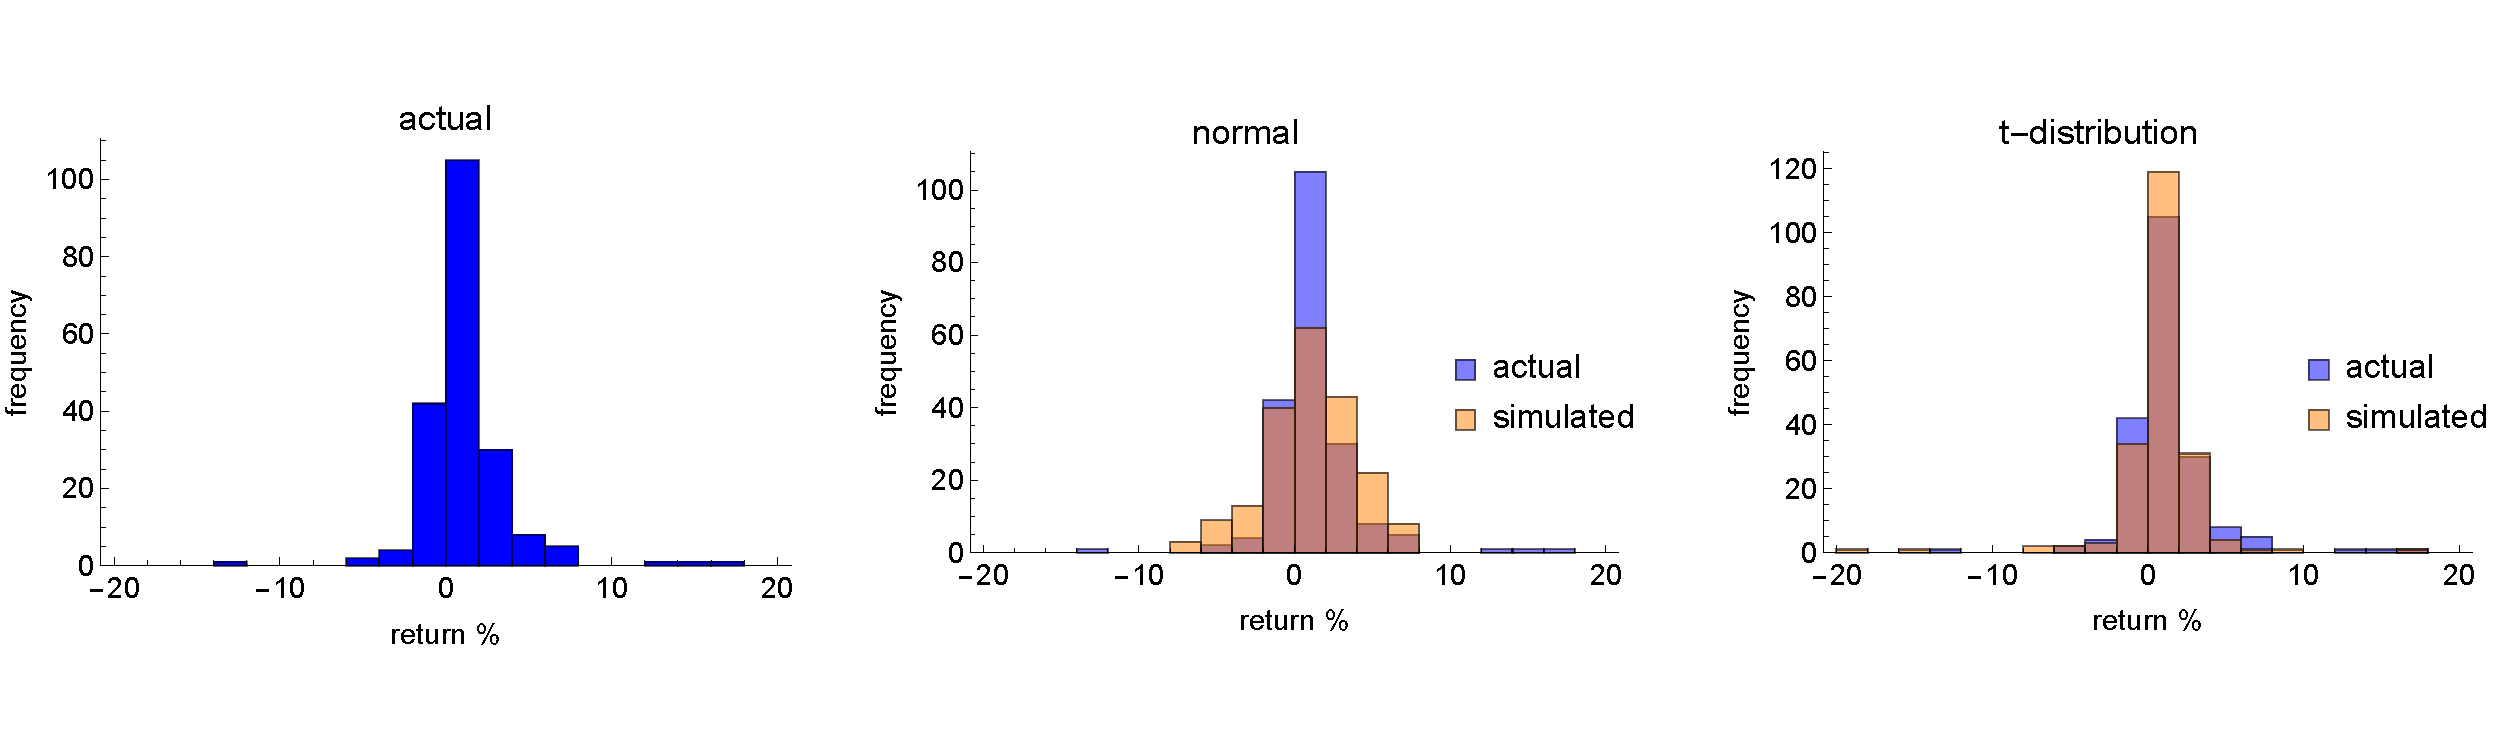
\includegraphics{Posterior_PPCstockReturns.pdf}}
\caption{Left: the actual data. Middle: actual returns vs normal-simulated returns. Right: actual returns vs t-distribution-simulated returns.}\label{fig:Posterior_PPCstockReturns}
\end{figure}


\section{Chapter summary}
In this chapter we have seen how the posterior distribution can be used to produce summaries of parameters. In particular, we have used these distributions to produce Bayesian credible intervals. We then compared and contrasted these with the classically-equivalent confidence interval, and have reasoned that in many cases the Bayesian formulation is more straightforward and intuitive than the former. We then move from the realm of the parameter, to that of the data, in order to produce prior and posterior data probabilities; which can be used to sense-check the implications of statistical models. We finally discussed methods of model comparison, introducing firstly the Bayes Factor method, followed by a short introduction to posterior predictive checks. Although the former method is common in the literature, we advocated the more nuanced approach of posterior predictive checks, albeit postponing more in-depth discussion until chapter \ref{chap:ModelFit}. Now that we have seen the utility of posterior probability distributions, we need to know how we can obtain them via Bayes' rule. In order to use the latter, we need to understand its constituent parts: the likelihood, prior and denominator. It is these three parts to which I devote the rest of the first part of this book.

\section{Chapter outcomes}
The reader should now be familiar with the following concepts:
\begin{enumerate}
\item Expressing uncertainty in a parameter's value through probability distributions.
\item The difference between the classical confidence interval and the Bayesian credible interval.
\item Summary measures of central tendency: posterior mean and median, and MAP. The issues with the latter.
\item How to obtain the prior and posterior predictive distributions from the prior and posterior distributions respectively.
\item Model evaluation through the posterior predictive distribution.
\end{enumerate}

\section{Problem set}
\subsection{The lesser evil}
Suppose that you are a neurosurgeon and have been given the unenviable task of finding the position of a tumour within a patient's brain, and cutting it out. Along two dimensions - height and left-right axis - the tumour's position is known to a high degree of confidence. However, along the remaining axis - front-back - the position is uncertain, and cannot be ascertained without surgery. However, a team of brilliant statisticians has already done most of the job for you, and has generated samples from the posterior for the tumour's location along this axis, and is given by the data contained within the data file "data\_Posterior\_PS\_tumour.csv" .

Suppose that the more brain that is cut, the more the patient is at risk of losing cognitive functions. Additionally, suppose that the damage inflicted varies:

\begin{enumerate}
\item Linearly with the distance the surgery starts away from the tumour.
\item Quadratically with the distance the surgery starts away from the tumour.
\item There is no damage if tissue cut is within 1mm of the tumour.
\end{enumerate}

Under each of the three regimes above, find the best position along this axis from which to belong the surgery?

\subsubsection{Which of the above loss functions do you think is most appropriate, and why?}
\subsubsection{Which loss function might you choose to be most robust to \textit{any} situation?}
\subsubsection{Following from the previous point, which measure of posterior centrality might you choose?}

\subsection{Google word search prediction}
Suppose you are chosen, for your knowledge of Bayesian statistics, to work at Google as a search traffic analyst. Based on historical data you have the data shown in table \ref{tab:Posterior_PS_googleInterval} for the actual word searched, and the starting string (the first three letters typed in a search). It is your job to help make the search engines faster, by reducing the search-space for the machines to lookup each time a person types.

\begin{table}[htbp]
  \centering
    \begin{tabular}{cccc}
    \toprule
          & \textbf{Barack Obama} & \textbf{Baby clothes} & \textbf{Bayes} \\
    \midrule
    \textbf{Bar} & 50\%  & 30\%  & 30\% \\
    \textbf{Bab} & 30\%  & 60\%  & 30\% \\
    \textbf{Bay} & 20\%  & 10\%  & 40\% \\
    \bottomrule
    \end{tabular}%
  \caption{The columns give the historic breakdown of the search traffic for three topics: Barack Obama, Baby clothes, and Bayes; by the first three letters of the user's search.}\label{tab:Posterior_PS_googleInterval}%
\end{table}%


\subsubsection{Find the minimum-coverage confidence intervals of topics that exceed 70\%.}
\subsubsection{Find most narrow credible intervals for topics that exceed 70\%.}

\subsubsection{Topic search volumes}
Now we suppose that your boss gives you the historic search information shown in table \ref{tab:Posterior_PS_googleIntervalHistoricTopic}. Further, you are told that what is most important is correctly suggesting the actual topic as one of the first auto-complete options irrespective of the topic searched.

Do you prefer confidence intervals or credible intervals in this circumstance?

\begin{table}[htbp]
  \centering
    \begin{tabular}{rccc}
    \toprule
          & \textbf{Barack Obama} & \textbf{Baby clothes} & \textbf{Bayes} \\
    \midrule
    \textbf{Search volume} & 60\%  & 30\%  & 10\% \\
    \bottomrule
    \end{tabular}%
  \caption{The historic search traffic broken down by topic.}\label{tab:Posterior_PS_googleIntervalHistoricTopic}%
\end{table}%

\subsubsection{Three-letter search volumes}
Alternatively, suppose that you have the historic search volume by the starting characters of the search, shown in table \ref{tab:Posterior_PS_googleIntervalHistoricKeyword}. You are now told, that the most important thing is directing the user to the correct topic given the keyword they have started to type.

Do you prefer confidence intervals or credible intervals in this circumstance?


\begin{table}[htbp]
  \centering
    \begin{tabular}{cccc}
    \toprule
          & \textbf{Bar} & \textbf{Bab} & \textbf{Bay} \\
    \midrule
    \textbf{Search volume} & 50\%  & 40\%  & 10\% \\
    \bottomrule
    \end{tabular}%
  \caption{The historic search traffic broken down by keyword.}\label{tab:Posterior_PS_googleIntervalHistoricKeyword}%
\end{table}%


\subsection{Prior and posterior predictive example (with PPCs maybe)}
Ben to add later.

\section{Appendix}
\subsection{The interval ENIGMA - explained in full}\label{sec:Posterior_appendixConfidenceInterval}


\chapter{Likelihoods}\label{chap:Likelihoods}
\begin{quotation}
The world is everything that is the case. \textbf{Wittgenstein}
\end{quotation}

\section{Chapter Mission statement}
At the end of this chapter a reader will know how to go about selecting a likelihood which is appropriate to a given situation. Further the reader will understand the basis behind maximum likelihood estimation.

Insert a graphic with the likelihood part of Bayes' formula circled, as in the equation shown below for the part highlighted in blue.

\begin{equation}
p(\theta|data) = \frac{{\color{blue}p(data|\theta)}\times p(\theta)}{p(data)}
\end{equation}\label{eq:Likelihood_BayesHighlighted}

\section{Chapter goals}
The starting point of the right hand side of the Bayesian formula is the likelihood function. This chapter will explain what is meant by a likelihood function, and why it is incorrect to view it as a probability in Bayesian analyses. The choice over which likelihood to use for a given situation is often difficult; especially to those unfamiliar with statistics. This chapter will provide practical guidance on likelihood choice, describing a framework that can be used to select a model in a systematic way. As an important stepping stone to Bayesian estimation, this chapter will also explain how classical maximum likelihood estimation works. 

\section{What is a likelihood?}
In all statistical inference, we use an idealised, simplified, model to try to mimic relationships between real variables of interest. This model is then used to test hypotheses about the nature of the relationships between these variables. In Bayesian statistics the evidence for a particular hypothesis is summarised in posterior probability distributions. Bayes' magic rule tells us how we can compute this posterior probability distribution for a given parameter within a model, $\theta$:

\begin{equation}
p(\theta|data) = \frac{p(data|\theta)\times p(\theta)}{p(data)}
\end{equation}\label{eq:Likelihood_Bayes}

The first step to understanding this formula (so that we can ultimately use it!) is to understand what is meant by the numerator term, $p(data|\theta)$, which Bayesians call a \textit{Likelihood}. Firstly, it's important to say that what we really mean by the numerator is:

\begin{equation}
p(data|\theta) = Probability(data|\theta,Model \; Choice)
\end{equation}\label{eq:Likelihood_simple}

(\ref{eq:Likelihood_simple}) represents the probability that we would have obtained the 'data', given (this is represented by the $|$ symbol) a particular value of $\theta$ and a particular choice of model. In other words, if our statistical model were true, and the value of the model's parameter were $\theta$, (\ref{eq:Likelihood_simple}) tells us the probability that we would have obtained our data. 

But what does this mean in simple, everyday language? Imagine that we flip a \textit{fair} coin. The most simple statistical model for coin flipping we can pick is to disregard the angle it was thrown at, as well as its height above the surface, along with any other details, and just pick the probability of the coin coming heads to be $\theta=\frac{1}{2}$. Furthermore, if a coin is thrown twice, we might choose to model the situation by assuming that the throwing technique is sufficiently similar between the two throws such that we can model each throw as independently having a probability of $\frac{1}{2}$. It's important to note that it is an assumption to forget about the throwing angle, as well as height of throw for each throw, and this forms part of our model of the situation. 

We can use our simple model\footnote{Albeit in practicality, this is a pretty reasonable representation of the situation for most purposes.} to calculate the probability that we obtain two heads in a row:

\begin{equation}
\begin{align}
Pr(HH|\theta,Model) &= Pr(H|\theta,Model)\times Pr(H|\theta,Model)\\
&= \theta \times \theta = \theta^2\\ 
&= \frac{1}{2}\times \frac{1}{2} = \frac{1}{4}
\end{align}
\end{equation}\label{eq:Likelihood_fairCoin}

The last row of (\ref{eq:Likelihood_fairCoin}) is obtained by assuming the probability of a head, $\theta=\frac{1}{2}$. If we continue to use this \textit{same} value of $\theta$, we can calculate the corresponding probabilities for all outcomes of throwing the coin twice. The most heads that can show up is 2, and the least being zero (if both flips come up tails). Figure \ref{fig:Likelihood_fairCoin} displays the probabilities for this model of the situation. The most likely number of heads to occur is 1, since this can occur in two different ways - either the first coin comes up heads, and the second is tails, or vice versa - whereas the other possibilities (all heads, or no heads) can each only occur in one way. However, the important thing to note about figure \ref{fig:Likelihood_fairCoin} isn't the individual probabilities, it is that it is a \textit{valid} probability distribution\footnote{See section \ref{sec:Probability_validProbabilityDistribution} for a refresher if you are unsure what is meant by a valid probability distribution.}, because:

\begin{itemize}
\item The individual event probabilities are all non-negative.
\item The sum of the individual probabilities is 1.
\end{itemize}

So it appears when we assume a particular value of $\theta$, and vary the data (in this case the number of heads obtained), the collection of resultant probabilities form a probability distribution. So, why do Bayesians call $p(data|\theta)$ a 'likelihood', and eschew the name 'probability'?

\begin{figure}
\centering
\scalebox{0.5} 
{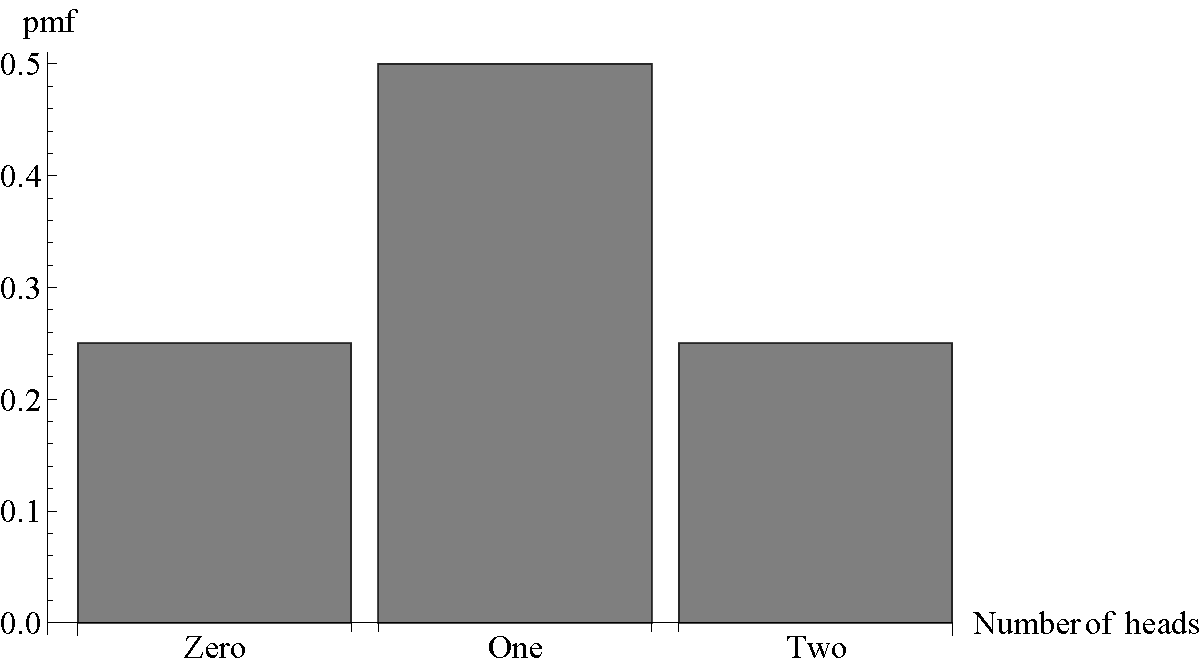
\includegraphics{Likelihood_fairCoin.pdf}}
\caption{The probabilities of all possible numbers of heads for a fair coin.}\label{fig:Likelihood_fairCoin}
\end{figure}

\section{Why use 'likelihood' rather than 'probability'?}
When we hold the parameters of our model fixed, as when we held the probability of an individual throw turning up heads, $\theta=\frac{1}{2}$, we've reasoned that the first term of the numerator of Bayes' rule in (\ref{eq:Likelihood_Bayes}) is a probability. So why don't we just keep calling it that, instead of renaming it a \textit{likelihood}? 

The reason is that in Bayesian inference, we \textit{don't} keep the parameters of our model fixed! In Bayesian analysis, it is the \textit{data} that is fixed, and the parameters that vary. This is because a posterior distribution shows the probability a parameter in a model lies in a particular range, assuming that we have obtained our particular data sample. For the case of a coin, where we don't know the probability of a head beforehand, what we hope to get out is a probability distribution of the kind shown in figure \ref{fig:Likelihood_posteriorExample}, where the x-axis is the value of $\theta$. In order to get $p(\theta|data)$ however, we must calculate $p(data|\theta)$ from the numerator of Bayes' rule in (\ref{eq:Likelihood_Bayes}) for each \textit{possible} value of $\theta$. If we assume we obtained one head and one tail, then we can calculate the probability of this occurring for a fixed $\theta$:

\begin{equation}
\begin{align}
Pr(HT|\theta) + Pr(TH|\theta) &= \theta(1-\theta) + \theta(1-\theta)
&= 2\theta(1-\theta)
\end{align}
\end{equation}

Since we are unsure as to the 'correct' value of $\theta$, we can graph this expression as a function of this parameter, to try to understand which values of the parameter are more or less likely, given our data (see figure \ref{fig:Likelihood_coinLikelihood}).

On first glances it appears that \ref{fig:Likelihood_coinLikelihood} could be a probability distribution, but first looks can be deceiving. 

\begin{figure}
\centering
\scalebox{0.5} 
{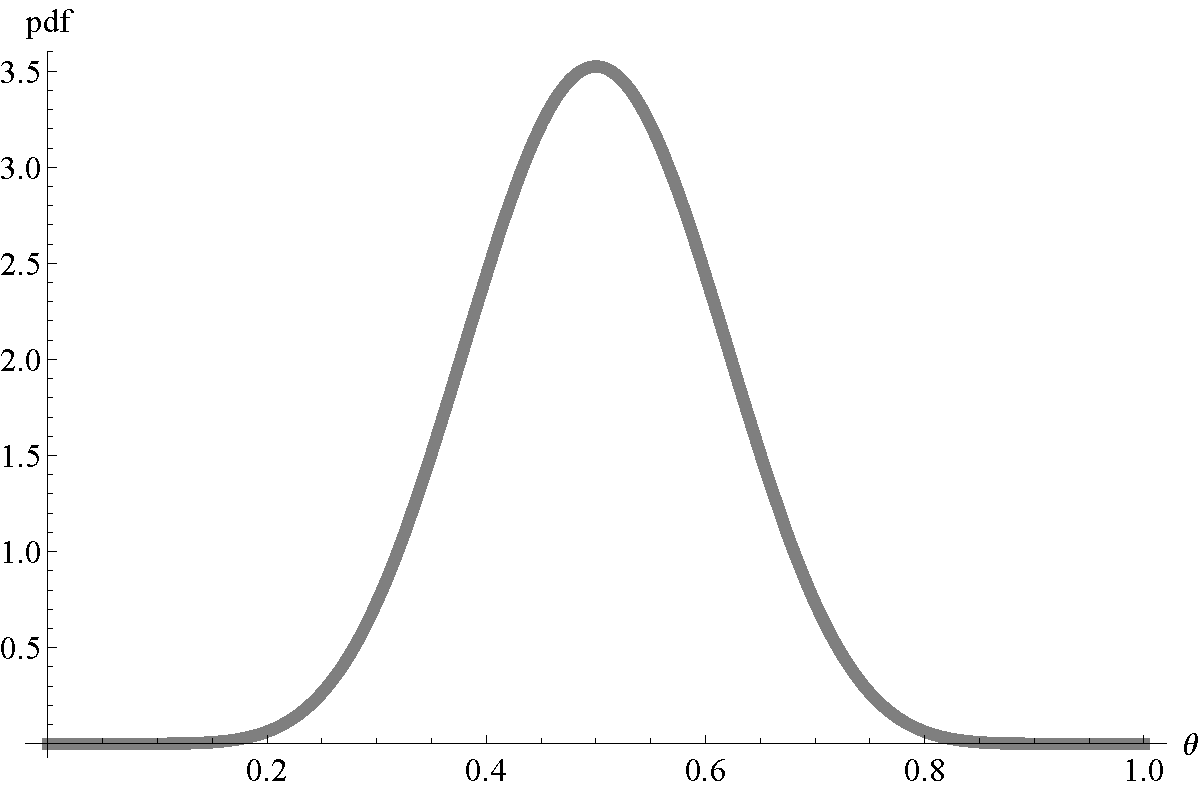
\includegraphics{Likelihood_posteriorExample.pdf}}
\caption{An example posterior distribution for the probability of obtaining a heads in a coin toss.}\label{fig:Likelihood_posteriorExample}
\end{figure}

\begin{figure}
\centering
\scalebox{0.5} 
{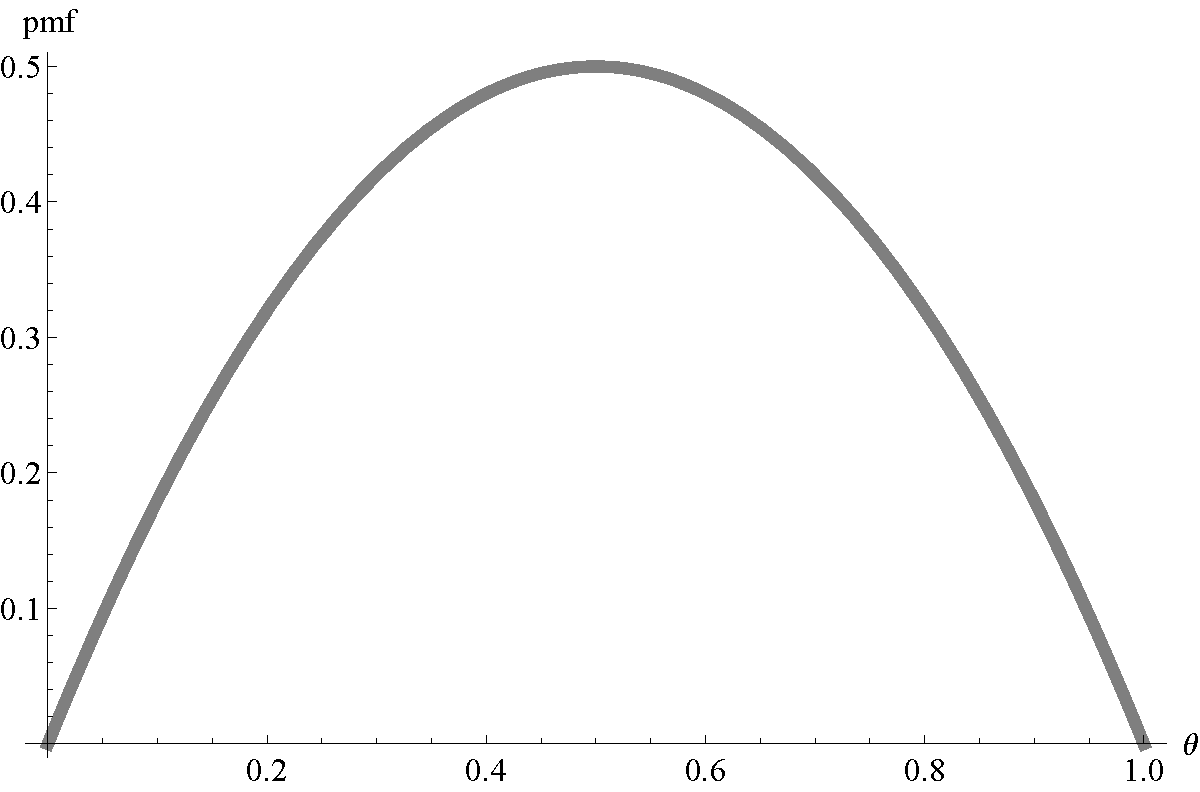
\includegraphics{Likelihood_coinLikelihood.pdf}}
\caption{The likelihood function for obtaining a single head from two throws. The area under the curve is $\frac{1}{3}$.}\label{fig:Likelihood_coinLikelihood}
\end{figure}

Checking off our necessary components of a probability distribution, we first note that all the values of the distribution in figure \ref{fig:Likelihood_coinLikelihood} are non-negative; which is what we require. However, if we calculate the area underneath the curve in figure \ref{fig:Likelihood_coinLikelihood}:

\begin{equation}
\mathrm{I} = \int\limits_{0}^{1} 2\theta(1-\theta)\mathrm{d}\theta = \frac{1}{3} \neq 1
\end{equation}

we find that it does not integrate to 1. Thus we have a violation of the second condition for a valid probability distribution. Hence, when we vary $\theta$ we find that, $p(data|\theta)$ is not a valid probability distribution! We thus introduce the term 'likelihood' to represent $p(data|\theta)$ when we vary the parameter, $\theta$. Often the following notation is used to emphasise that likelihood is a function of the parameter $\theta$ with the data held fixed:

\begin{equation}\label{eq:Likelihood_notation}
\mathcal{L}(\theta|data) = p(data|\theta)
\end{equation}

However, in this book, we will persist with the original notation as this is most typical in the literature, under the implicit assumption that when we vary the parameters in question, the term is not strictly a probability.

To provide further justification for this argument, consider the following (albeit contrived) example. Suppose that, we throw a coin twice, and we are told beforehand that the probability of obtaining a head on a particular throw is one of six discrete values: $\theta\in\{0.0,0.2,0.4,0.6,0.8,1.0\}$. We can then use our model to calculate the probability of obtaining a number of heads, $X$:

\begin{align}\label{eq:Likelihood_OneHead}
Pr(X = 0|\theta)& = Pr(TT|\theta) = Pr(T|\theta)\times Pr(T|\theta) = (1-\theta)^2\\
Pr(X = 1|\theta)& = Pr(HT|\theta) + Pr(TH|\theta) = 2\times Pr(T|\theta)\times Pr(H|\theta) = 2\theta(1-\theta)\\\label{eq:Likelihood_TwoHead}
Pr(X = 2|\theta)& = Pr(HH|\theta) = Pr(H|\theta)\times Pr(H|\theta) = \theta^2
\end{align}

In (\ref{eq:Likelihood_OneHead}), the probability is simply given by the product of the probabilities of not obtaining a head on the first throw, $(1-\theta)$, by the probability of not obtaining a head in the second\footnote{Since we have assumed a model whereby the results of the first and second throws are independent, conditional on $\theta$. In other words, all the similarity between the two throws is captured in the parameter $\theta$.}, which is also $(1-\theta)$. The factor of two arises in (\ref{eq:Likelihood_TwoHead}) since there are two ways of getting one head: \{HT,TH\}.

We can represent the corresponding values of likelihood/probability as is shown in table \ref{tab:Likeihood_BayesBox}. In this form we can see the impact of varying the data (moving along each row), and contrast it with the effect of varying $\theta$ (moving down each column). Note that if we hold the parameter fixed - regardless of this initial choice of $\theta$ - and move along each row summing the entries, we find that the values sum to 1; meaning that this is a valid probability distribution. By contrast, when we hold the number of heads fixed, and vary the parameter $\theta$, moving down each column, summing the entries, we find that the values do not sum to 1. Hence, when we vary $\theta$, we are not dealing with a proper probability distribution, meriting the use of the term 'likelihood'.

In Bayesian inference, we always vary the parameter, and implicitly hold the data fixed. Thus, from a Bayesian perspective it is important to use the term \textit{likelihood} to indicate that we recognise we are not dealing with a probability distribution.


\begin{table}[htbp]
  \centering
  
    \begin{tabular}{ccccc}
    \multicolumn{5}{c}{\textbf{Number of heads}} \\
    \midrule
    \textbf{$\theta$} & \multicolumn{1}{c}{\textbf{0}} & \multicolumn{1}{c}{\textbf{1}} & \multicolumn{1}{c}{\textbf{2}} &  \multicolumn{1}{c}{\textbf{Total}} \\
    \hline
    \textbf{0.0} & \multicolumn{1}{c}{1.00} & \multicolumn{1}{c}{0.00} & \multicolumn{1}{c}{0.00} & \multicolumn{1}{c}{\textbf{1.00}} \\
    \textbf{0.2} & \multicolumn{1}{c}{0.64} & \multicolumn{1}{c}{0.32} & \multicolumn{1}{c}{0.04} & \multicolumn{1}{c}{\textbf{1.00}} \\
    \textbf{0.4} & \multicolumn{1}{c}{0.36} & \multicolumn{1}{c}{0.48} & \multicolumn{1}{c}{0.16} & \multicolumn{1}{c}{\textbf{1.00}} \\
    \textbf{0.6} & \multicolumn{1}{c}{0.16} & \multicolumn{1}{c}{0.48} & \multicolumn{1}{c}{0.36} & \multicolumn{1}{c}{\textbf{1.00}} \\
    \textbf{0.8} & \multicolumn{1}{c}{0.04} & \multicolumn{1}{c}{0.32} & \multicolumn{1}{c}{0.64} & \multicolumn{1}{c}{\textbf{1.00}} \\
    \textbf{1.0} & \multicolumn{1}{c}{0.00} & \multicolumn{1}{c}{0.00} & \multicolumn{1}{c}{1.00} & \multicolumn{1}{c}{\textbf{1.00}} \\
    \bottomrule
    \textbf{Total} & \multicolumn{1}{c}{\textbf{1.20}} & \multicolumn{1}{c}{\textbf{1.60}} & \multicolumn{1}{c}{\textbf{2.20}} &  \\
    
    \end{tabular}%
  %
  \caption{The values of likelihood for the case of tossing a coin twice, where the probability of heads is constrained to take on a discrete value: \{0.0,0.2,0.4,0.6,0.8,1.0\}.}\label{tab:Likeihood_BayesBox}
\end{table}

\section{What are models and why do we need them?}
All models are wrong. They are idealised representations of reality resultant from making assumptions, which if reasonable, may emulate some of the behaviour of a system of interest. Joshua Epstein in an article titled, 'Why model?' emphasises that we perennially build \textit{implicit} mental models for various phenomena \cite{epstein2008model}. Before we go to bed at night we set our alarms for the next morning on the basis of a model. We imagine an idealised - model - morning when it takes us 15 minutes to wake up as a result of an alarm. We use this model to predict how long it will take us to rise from bed, shower, and get changed into clothes in sufficient time to get to work. Whenever we go to the Doctor, they use an internalised biological model of the human body to advise on the best course of treatment for a particular ailment. Whenever we hear expert opinions on TV about the outcome of an upcoming election, the pundits are using mental models of society to explain the results of current polls, as well as make forecasts. As is the case with all models, some are better than others. Hopefully, the models a Doctor uses to prescribe medicine are subject to less error than the opinions of pundits seen on TV\footnote{For a great discussion of the performance of TV pundits, read Thinking Fast. Insert reference}! 

Epstein goes on to emphasise that the question, 'Why model?' really means why should we build an \textit{explicit} - written down - model of phenomena? The point being that \textit{implicit} models are by their very nature, opaque, and not subject to the sort of interrogation that can be obtained by writing the model on paper. 

We can also ask more narrowly, what are we hoping to gain by building an \textit{explicit} model of a situation? Epstein suggests the following motivations:

\begin{itemize}
\item Prediction
\item Explanation
\item Guide data collection
\item Discover new questions
\item Bound outcomes to plausible ranges
\item Illuminate uncertainties
\item Challenge the robustness of prevailing theory through perturbations
\item Reveal the apparently simple (complex) to be complex (simple) 
\end{itemize}

There are of course other reasons to build models, but we believe that this list is a reasonable starting point. However, we should not think of this list as static. Whenever we build a model, whether it is statistical, biological or sociological, we should ask, 'What are we hoping to gain by building this model, and how can I judge its success?'. Only when we have a grasp on the answers to these basic questions should we proceed to model building.

\section{How to choose an appropriate likelihood?}\label{sec:chooseLikelihood}
Bayesians are acutely aware that their models are wrong. At best the abstraction from reality allows us to explain some aspect of real behaviour; at worst they can be very misleading. Before we use a model for prediction, we require that it can explain some reasonable proportion of the system's behaviour for the past and present. With this in mind we introduce the following model selection framework:

\begin{enumerate}
\item Write down the real life behaviour/data patterns that the model should be capable of explaining.
\item Write down the assumptions that it is believed are reasonable in order to achieve the above point.
\item Search the literature for models which utilise these assumptions; extracting only the relevant components.
\item Test your model's ability to explain said behaviour/data patterns. If unsuccessful go back to the second step and re-evaluate the appropriateness of your assumptions.
\end{enumerate}

Whilst this methodology is useful for building a statistical model in general, it is more applicable for use with a full Bayesian model, resulting in a posterior distribution. In which case how do we go about specifying a likelihood for a given situation? To answer this we will start with going through a simple example.

\subsection{A likelihood model for an individual's disease status}\label{sec:Likelihood_individualDisease}
Suppose we work for the State as a healthcare analyst, and we want to build a statistical model to explain the prevalence of a certain disease within a sample, which can then be used to make inferences about the population incidence. Also, (unrealistically) let's imagine that we start off with a sample of only one person, for whom we have no prior information. Let the disease status of that individual be denoted by the variable $X$ which takes on the following binary outcome values dependent on the disease status the individual:

\begin{equation}
X =
\begin{cases}
O & , No\; disease \\
1 & , Positive \; diagnosis
\end{cases}
\end{equation}

The goal of our model is to output a probability that this individual has the disease. We might assume that a fraction $\theta$ of the population has the disease, and that this individual has come from that population. For each possible outcome, we can use this simple model to calculate the probability of each outcome:

\begin{align}\label{eq:Likelihood_SimpleModel1}
Pr(X = 0|\theta)& = (1-\theta)\\
Pr(X = 1|\theta)& = \theta\label{eq:Likelihood_SimpleModel2}
\end{align}

Note the similarity between these probabilities and those of the coin flipping example in the previous section. Often, a given model can be reused in a multitude of different settings.

However, we would like to write down a single rule which yields (\ref{eq:Likelihood_SimpleModel1}) or (\ref{eq:Likelihood_SimpleModel2}) respectively, dependent on whether $X=0$ or $X=1$. This can be achieved with the following:

\begin{equation}\label{eq:Likelihood_bernoulli}
Pr(X=\alpha|\theta) = \theta^\alpha(1-\theta)^{1-\alpha}
\end{equation}

Note that in (\ref{eq:Likelihood_bernoulli}) that $\alpha\in\{0,1\}$ refers to the numeric value taken by the variable $X$. The function (\ref{eq:Likelihood_bernoulli}) is known as a \textit{Bernoulli} probability density.

Although this rule for calculating a probability of a particular disease status, $\alpha$, looks complex, we see that it reduces to (\ref{eq:Likelihood_SimpleModel1}) and (\ref{eq:Likelihood_SimpleModel2}) if the individual is disease -negative/-positive respectively:

\begin{align}\label{eq:Likelihood_SimpleModel3}
Pr(X = 0|\theta)& = \theta^0(1-\theta)^1 = (1-\theta)\\
Pr(X = 1|\theta)& = \theta^1(1-\theta)^0 = \theta\label{eq:Likelihood_SimpleModel4}
\end{align}

When we hold the datum $X$ fixed and vary $\theta$, (\ref{eq:Likelihood_bernoulli}) represents a likelihood. However, figure \ref{fig:Likelihood_bernoulli} shows that for a fixed value of $theta$ the sum (here we mean the vertical sum) of the two probability densities is always equal to 1; demonstrating that in this case (\ref{eq:Likelihood_bernoulli}) is a valid probability density. Notice also in figure \ref{fig:Likelihood_bernoulli} that the sum of probability density is defined continuously on $\{0,1\}$, whereas the sum of likelihoods is discrete.

\begin{figure}
\centering
\scalebox{0.75} 
{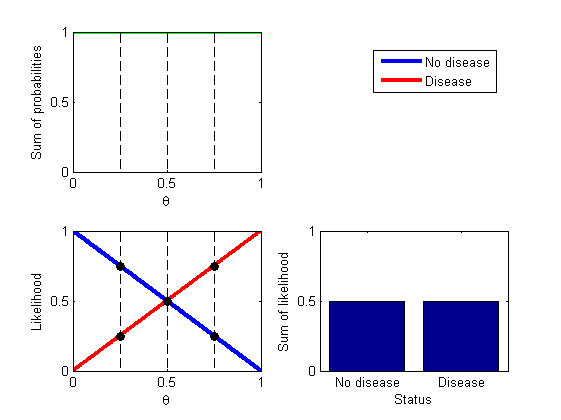
\includegraphics{likelihood_bernoulli.png}}
\caption{The likelihood function as theta varies for the case of the two possible data. The sum of likelihoods is found by the area under each line, whereas the sum of probabilities is a discrete sum.}\label{fig:Likelihood_bernoulli}
\end{figure}

\subsection{A likelihood model for disease prevalence of a group}\label{sec:Likelihood_diseaseGroup}
Now we imagine that instead of this solitary individual, we have a group of $N$ individuals. What we would like to do is to calculate the develop a model which will tell us the probability of obtaining $Z$ disease cases within our sample. We would also like to be able to use our model to predict the most likely number of individuals who have the disease in a sample, for a given value of the parameters\footnote{We are starting off by assuming that we know the parameters. Later in this chapter we will obtain a point estimate of the parameters using \textit{Maximum likelihood} estimation.}. 

In order to write down a model we first need to make some simplifying assumptions. We might assume that one individual's disease status tells us nothing about the probability of another individual in the sample having the disease\footnote{Other than, if the disease prevalence were unknown, through our ability to estimate overall disease prevalence from their individual statuses.}. This would not be a reasonable assumption if the disease were contagious, and if the individuals in the sample came from the same neighbourhood or household. It also would not be a good assumption if (as is often the case with volunteer-dependent studies) the individuals who volunteered for the experiment, self-selected on the basis of some common pre-existing ailment/underlying-factor. If an advert for participants reads, 'Psychological experiment on sleep disorders: participants wanted', we might suspect that there would be an over-presence of insomniacs than is found in the population as a whole. This first assumption is that which in statistical language we call 'independence'. We also suppose that all individuals in our sample come from the same population - the one we are trying to draw conclusions about. If we knew beforehand that some individuals came from different populations, with significantly different prevalence rates, then we might abandon this assumption. Combining these two assumptions we say in statistical language that our data sample is \textit{independent} and \textit{identically-distributed}.

With our two assumptions in hand, we can begin to formulate a model for the probability of obtaining $Z$ disease-positive individuals out of a total of $N$ individuals. We start by considering each person's disease status individually, meaning we can reuse (\ref{eq:Likelihood_bernoulli}):

\begin{equation}\label{eq:Likelihood_bernoulli1}
Pr(X=\alpha|\theta) = \theta^\alpha(1-\theta)^{1-\alpha}
\end{equation}

Note that in (\ref{eq:Likelihood_bernoulli1}) the $\alpha\in\{0,1\}$ refers to a particular numeric value taken by the variable $X$. The assumption of \textit{independence} means that we can get the overall probability by multiplying together the individual probabilities\footnote{See section \ref{sec:Probability_independence} for an explanation of this.}. In words, we obtain the probability that the first person has disease status $X_1$ \textit{and} the second person has status $X_2$:

\begin{equation}\label{eq:Likelihood_bernoulli2}
\begin{align}
Pr(X_1=\alpha_1,X_2=\alpha_2|\theta_1,\theta_2) &= Pr(X_1=\alpha_1|\theta_1)\;\times \;Pr(X_2=\alpha_2|\theta_2)\\
 &= \theta_1^{\alpha_1}(1-\theta_1)^{1-\alpha_1}\times \theta_2^{\alpha_2}(1-\theta_2)^{1-\alpha_2}
\end{align}
\end{equation}

In (\ref{eq:Likelihood_bernoulli2}) we have assumed that each individual has a different predisposition to having the disease, denoted by $\theta_1$ and $\theta_2$ respectively.

The second assumption of \textit{identically-distributed} individuals means that we can set $\theta_1=\theta_2$:

\begin{equation}\label{eq:Likelihood_bernoulli3}
\begin{align}
 Pr(X_1=\alpha_1,X_2=\alpha_2|\theta) &= \theta^{\alpha_1}(1-\theta)^{1-\alpha_1}\times \theta^{\alpha_2}(1-\theta)^{1-\alpha_2}\\
&= \theta^{\alpha_1+\alpha_2}(1-\theta)^{2-\alpha_1-\alpha_2}
\end{align}
\end{equation}

In (\ref{eq:Likelihood_bernoulli3}) we have obtained the second line by using the simple exponent rule: $a^b\times a^c = a^{b+c}$, for the components $\theta$ and $(1-\theta)$ respectively.

For our sample of 2 we are now in a position to calculate the probability that we obtain $Z$ cases of the disease. We first realise that we can get from $X_1$ and $X_2$ to $Z$ by:

\begin{equation}\label{eq:Likelihood_binomialTwo}
Z = X_1 + X_2
\end{equation}

We can then use (\ref{eq:Likelihood_bernoulli3}) to generate the respective probabilities.

\begin{equation}\label{eq:Likelihood_binomialTwoProbs}
\begin{align}
Pr(Z = 0|\theta)& = Pr(X_1=0,X_2=0|\theta) = \theta^{0+0}(1-\theta)^{2-0-0} = (1-\theta)^2\\
Pr(Z = 1|\theta)& = Pr(X_1=1,X_2=0|\theta) + Pr(X_1=0,X_2=1|\theta)= 2\theta(1-\theta)\\
Pr(Z = 2|\theta)& = Pr(X_1=1,X_2=1|\theta) = \theta^{1+1}(1-\theta)^{2-1-1} = \theta^2
\end{align}
\end{equation}

To complete our probability model we want to write out a single rule for calculating the probability of any value taken on by $Z$. To do this we note that we could rewrite (\ref{eq:Likelihood_binomialTwoProbs}) as:

\begin{equation}\label{eq:Likelihood_binomialTwoProbsSimple}
\begin{align}
Pr(Z = 0|\theta)& = \;\theta^0(1-\theta)^2\\
Pr(Z = 1|\theta)& = 2\theta^1(1-\theta)^1\\
Pr(Z = 2|\theta)& = \;\theta^2(1-\theta)^0
\end{align}
\end{equation}

In (\ref{eq:Likelihood_binomialTwoProbsSimple}) we notice the common term $\theta^\beta (1-\theta)^{2-\beta}$ in each of the expressions, where $\beta\in\{0,1,2\}$ represents the number of disease cases found. Therefore this suggests that we may be able to write down a single rule as something similar to:

\begin{equation}\label{eq:Likelihood_binomialNearly}
Pr(Z = \beta|\theta) \sim \theta^\beta(1-\theta)^{2-\beta}
\end{equation}

The only problem with matching (\ref{eq:Likelihood_binomialNearly}) with the previously obtained result is the factor of 2 on the middle line of (\ref{eq:Likelihood_binomialTwoProbsSimple}). However, as a complete aside we note that when we expand a quadratic factor we get the following:

\begin{equation}\label{eq:Likelihood_quadratic}
(x+1)^2 = x^2 + 2x + 1
\end{equation}

The numbers $\{1,2,1\}$ correspond here to the non-b-dependent coefficients of $\{x^2,x^1,x^0\}$ respectively. This sequence of numbers normally appears in early secondary school maths classes, and is either known as the binomial expansion coefficients or simply $^nC_r$. The expansion coefficients are normally written in compact form:

\begin{equation}\label{eq:Likelihood_nCr}
{2 \choose \beta} = \frac{2!}{(2-\beta)!\beta!}
\end{equation}

In (\ref{eq:Likelihood_nCr}) the $!$ has its usual meaning of factorial, and $\beta\in\{0,1,2\}$. We can therefore use this notation to help us to write down a single model for the probability of obtaining $Z$ disease cases out of a total of 2 individuals using our model:

\begin{equation}\label{eq:Likelihood_binomialTwoFull}
Pr(Z=\beta|\theta) = {2 \choose \beta} \theta^\beta (1-\theta)^{2-\beta}
\end{equation}

This likelihood function is illustrated for the three possible numbers of disease cases in figure \ref{fig:Likelihood_binomial}.

\begin{figure}
\centering
\scalebox{0.75} 
{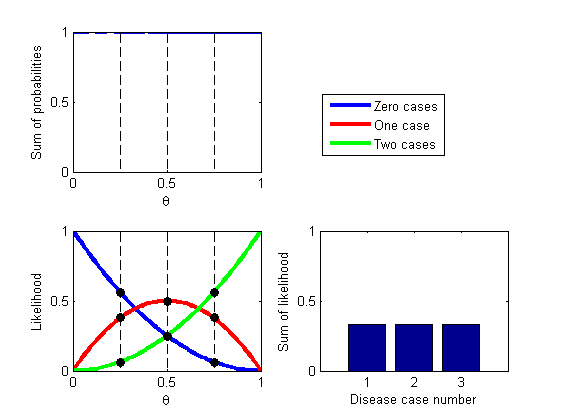
\includegraphics{likelihood_binomial.png}}
\caption{The likelihood function as theta varies for a sample of 2 individuals.}\label{fig:Likelihood_binomial}
\end{figure}

We will now extend the analysis to cover the case when we have groups of $N$ individuals. Firstly, consider the case when we have a group size of 3. If we assume that the individuals are identically distributed, then the 4 probabilities are of the form:

\begin{equation}\label{eq:Likelihood_binomialThreeProbsSimpler}
\begin{align}
Pr(Z = 0|\theta)& = \;Pr(X_1=0|\theta) Pr(X_2=0|\theta)  Pr(X_3=0|\theta)\\
Pr(Z = 1|\theta)& = 3Pr(X_1=1|\theta) Pr(X_2=0|\theta)  Pr(X_3=0|\theta)\\
Pr(Z = 2|\theta)& = 3Pr(X_1=1|\theta) Pr(X_2=1|\theta)  Pr(X_3=0|\theta)\\
Pr(Z = 3|\theta)& = \;Pr(X_1=1|\theta)Pr(X_2=1|\theta) Pr(X_3=1|\theta)
\end{align}
\end{equation}

Again, we notice a numeric pattern in terms of the first part of each expression $\{1,3,3,1\}$, which happens to correspond exactly to the coefficients on terms for the expansion of $(x+1)^3$. Hence, we can again rewrite the likelihood using the binomial expansion notation:

\begin{equation}\label{eq:Likelihood_binomialThreeFull}
Pr(Z=\beta|\theta) = {3 \choose \beta} \theta^\beta (1-\theta)^{3-\beta}
\end{equation}

We recognise a pattern in the likelihoods of (\ref{eq:Likelihood_binomialTwoFull}) and (\ref{eq:Likelihood_binomialThreeFull}) which allows us to deduce that, for a sample size of N, the likelihood is given by:

\begin{equation}\label{eq:Likelihood_binomialNFull}
Pr(Z=\beta|\theta) = {N \choose \beta} \theta^\beta (1-\theta)^{N-\beta}
\end{equation}

(\ref{eq:Likelihood_binomialNFull}) is known as the \textit{binomial} probability distribution.

If we had data, then we could test whether the assumptions made were appropriate by calculating the model-implied-probability of this outcome. For example, if we had a sample of 100 people of which 10 were disease-positive, and we assumed beforehand that the proportion of the population who have the disease is $\theta=1\%$, then we could calculate the probability that we would have achieved a number of cases as bad, or worse than this using (\ref{eq:Likelihood_binomialNFull}):

\begin{equation}
Pr(Z\geq 10|\theta=0.01) = \sum\limits_{Z=10}^{100}{100 \choose Z} 0.01^Z (1-0.01)^{100-Z} = 7.63 \times 10^{-8}
\end{equation}\label{eq:Likelihood_binomialTest}

We have summed over all the disease cases from 10 to 100 here, because we wanted the probability that we would have obtained a result as bad, or worse, than the one which we actually achieved. This is a particular way of carrying out classical hypothesis tests, which we will dispense with later on, but for now it seems a reasonable way of testing our model. 

The probability found in this case is extremely small. What does this tell us? Well, it basically says that there is something wrong with our model which we have chosen here. It could be that the actual disease incidence in the population is much higher than the 1\% which we have assumed beforehand. It could also be that our assumption of  \textit{independence} is violated in this case, for example if we sampled whole households rather than individuals. This could mean that in a particular household, the chance of having the disease, if another member of your family has the disease, is substantially higher than for the population as a whole. 

It is difficult to gauge what in particular is wrong with our model without knowing further details of data collection, as well as how the estimate of 1\% incidence was estimated for the population. However, it does suggest that we need to do adjust one or more of our assumptions, and reformulate the model to take these into account. We should never simply accept that our model is \textit{correct}. A model is only as good as its capability to reproduce the data which we see in real life. In this case we find it is not a good representation, and we should readjust appropriately.

\subsection{The intelligence of a group of people}\label{sec:Likelihood_normal}
We are now tasked with formulating a model of intelligence test scores for a group of individuals for whom we have data. We are told that the test score is on a continuous scale from 0-200. We do not have any information on individual characteristics which might help us to predict scores, although we are going to, for this simplified example, assume that we do know the mean test score $\mu=70$, and its variance $\sigma^2=81$ in the population (although we will relax this assumption in section \ref{sec:Likelihood_MLE}). We might assume that there are a range of factors which overall result in an individual's performance on this test. For example, these might include their schooling, parental education, 'innate' ability, as well as how tired they were feeling on the day of the test. If we assume that there are a large range of such factors and the score which results is an average of all these, then we might assume that the Central Limit Theorem might be appropriate for determining the distribution of test scores\footnote{See section \ref{sec:Probability_CLT} for an introduction to the Central Limit Theorem.}. In which case, we assume that a normal distribution for our likelihood function for an individual's test score, $X$:

\begin{equation}
p(X=\alpha|\mu,\sigma^2) = \frac{1}{\sqrt{2\pi\sigma^2}}e^{-\frac{(\alpha-\mu)^2}{2\sigma^2}}
\end{equation}\label{eq:Likelihood_normal}

Note that since this distribution is continuous, we have written $p$ rather than $Pr$. The first $p$ represents a density, whereas $Pr$ represents a probability, which is only found in the continuous case by integrating over some bounds.

\begin{figure}
\centering
\scalebox{0.35} 
{\includegraphics{likelihood_normal.pdf}}
\caption{Left panel shows a normal with $\mu=70$ and $\sigma^2 = 81$, with the area corresponding to a result as extreme as 90 indicated. This translates into a standard normal cdf shown in the right panel, which can be used to calculate this area from the first figure. This translation to the standard normal is done by taking away $\mu$, and dividing through by $\sigma$. This is done since usually only standard normal cdf tables are available.}\label{fig:Likelihood_normal}
\end{figure}

If we obtain an individual within our sample who achieved a test score of 90, we ask what's the probability of achieving a result as extreme as this? Using our idealised model, we just integrate the probability density (this is the continuous analogue to the discrete summing that we did in (\ref{eq:Likelihood_binomialTest})):

\begin{equation}
\begin{align}
Pr(X\geq 90|\mu=70,\sigma^2=81) &= \int\limits_{90}^{\infty}\frac{1}{\sqrt{2\pi\times 10}}e^{-\frac{(\alpha-70)^2}{2\times 10}} \mathrm{d}\alpha\\
 & = 1-\Phi\left(\frac{90-70}{9}\right) \approx 0.0131
\end{align}\label{eq:Likelihood_normalSampleOne}
\end{equation}

In (\ref{eq:Likelihood_normalSampleOne}), $\Phi$ stands for the value of the \textit{standard} normal cumulative distribution function\footnote{A standard normal has mean 0, and a variance of 1. By taking away the mean of 70, and dividing through by the standard deviation, we transform from an arbitrary mean- and variance-normal, to a \textit{standard} one.} at the value of 90 (see figure \ref{fig:Likelihood_normal} for an explanation). Since we find that the probability of obtaining this data point under our current model is extremely small, we conclude that it is likely that there is something wrong with our model, and go back to examine the various assumptions that were made in deriving it.

If we also assume that information regarding one individual's test score tells us nothing about another's\footnote{Apart from their joint reliance on $\mu$ and $\sigma^2$.}, then we might assume \textit{independence} for our data. We might also assume that all individuals come from the same population; resulting in a \textit{random sample}\footnote{See section \ref{sec:Likelihood_randomSampleExchangeable} for further discussion of random samples.}. We calculate the joint probability density for a sample of N individuals by multiplying together the individual densities:


\begin{equation}
P(X_1=\alpha_1,X_2 =\alpha_2,...,X_N=\alpha_N|\mu,\sigma^2) = \prod\limits_{i=1}^{N}\frac{1}{\sqrt{2\pi\sigma^2}}e^{-\frac{(\alpha_i-\mu)^2}{2\sigma^2}}
\end{equation}\label{eq:Likelihood_normalN}


We could then use (\ref{eq:Likelihood_normalN}) to calculate the probability of obtaining a given sample of observations as extreme as the values obtained, again by integrating. However, here it would be slightly more complicated than that of (\ref{eq:Likelihood_normalSampleOne}) since we would have to integrate across all individuals' variables.

\section{Exchangeability vs random sampling}\label{sec:Likelihood_randomSampleExchangeable}
We have already been introduced to the concept of a \textit{random sample}, in developing a probability model for the disease status of patients (section \ref{sec:Likelihood_diseaseGroup}), and the intelligence of a group of people (see section \ref{sec:Likelihood_normal}). The use of this term is really just a shorthand for an \textit{independent}, and \textit{identically-distributed} sample of data. Often however, Bayesians eschew this term in want of a (slightly) weaker condition that still allows us to write down an overall likelihood as a product of individual likelihoods in many situations. 

Suppose we have a sequence of random variables representing the height of individuals in a sample of size 3: $\{H_1,H_2,H_3\}$. If this sequence is as likely as the reordered sequence: $\{H_2,H_1,H_3\}$, or any other re-ordering, then the sequence is said to be \textit{exchangeable}\footnote{Formally, a sequence which is exchangeable requires that the joint probability distribution is invariant under any permutation of the order.}.

Since the assumption of random sampling is stronger than that of exchangeability, it turns out that any random sample is automatically exchangeable. However, the converse is not necessarily true. A particular example of this is for the case of an urn containing 3 red and 3 blue balls, which are drawn at random without replacement. The probability of obtaining the sequence $RBR$ is given by:

\begin{equation}
Pr(RBR) = \frac{3}{6} \times \frac{3}{5} \times \frac{2}{4} = \frac{3}{20}
\end{equation}

The sequence of random variables representing the outcome of this sampling \textit{is} exchangeable, since we have that any permutation of this sequence is equally likely:

\begin{equation}
\begin{align}
Pr(BRR) &= \frac{3}{6} \times \frac{3}{5} \times \frac{2}{4} &= \frac{3}{20}\\
Pr(RRB) &= \frac{3}{6} \times \frac{2}{5} \times \frac{3}{4} &= \frac{3}{20}
\end{align}
\end{equation}

However, this sequence of random variables is \textit{not} a random sample. The probability distribution for the first ball drawn is different to that when the second is drawn. In the first case there are 6 balls in total, with equal numbers of each. However, for the second case there are only 5 balls, and \textit{dependent} on the first draw, there may be either more red balls or blue balls remaining.

In general we may not be able to assume we have a conditional\footnote{Conditional on a distribution of a vector of parameters $\theta$ which sits above all the observations.} random sample of observations for reasons similar to that of the urn example. However, a brilliant theory originally by Bruno de Finetti allows us to assume that a sequence behaves as if it is a random sample, \textit{so long as it is exchangeable.} Technically this requires that we need an infinite sample of observations, but for a reasonably large sample making this approximation is reasonable.

Much of the time we will have a random sample, and so do not need to worry about any of this. However, due to this theorem, we are often free to write down an overall likelihood as the product of individual likelihoods, so long as the observations are exchangeable.

\section{The subjectivity of model choice}
It is hoped that the analysis in the preceding sections has given us a taste of how we can go about specifying a likelihood for a hitherto unknown circumstance. We start by writing down the behaviours that we want to emulate, then make simplifying assumptions, which we then use to look for an appropriate model in the literature. This model is then used to test the validity of the assumptions with the sample data. If the model struggles to explain the data, then we should go back and iteratively modify, then test our model, until it adequately explains the range of behaviours.

However, it should be re-emphasised that by its nature, a model is always a simplification of reality. As such, no one model is \textit{correct}. There are often many models that could be used to explain the data which we have to hand. We should always take care to test each of these against its ability to explain the aspect of the data in which we are interested, and only proceed with it if it is adequate in this regard. Real life is complicated, and thus with each of the assumptions that were used to justify a particular model, there will inevitably be a degree of \textit{subjectivity}. As such, no analysis - whether Frequentist or Bayesian - can be thought to be purely \textit{objective}. Hence, the human analyst cannot, and should not, be replaced by automata for statistical analysis. A degree of subjective judgement is always necessary in statistics, as in all other walks of life.

\section{Maximum likelihood - a short introduction}\label{sec:Likelihood_MLE}
The analysis in section \ref{sec:chooseLikelihood} assumes that we know beforehand the fraction, $\theta$, of the populous that are predisposed to having the disease. In reality we rarely know such a thing. Often the main focus of building a statistical model is to try to estimate such parameters from our sample of data to which we have access. A popular Frequentist method for achieving this goal is the estimation strategy known as \textit{Maximum Likelihood}. In this section we will examine how this estimation strategy yields estimates of parameters.

The principle of Maximum Likelihood estimation is simple. Firstly, we assume a model which we use to approximate the data generating process which resulted in our sample, based on the various assumptions about the real life process which we make. We then calculate what is known as the joint probability of obtaining the sample of observations, assuming that we do not know the parameters which specify completely those distributions. We then choose the parameters which \textit{maximise} the likelihood of obtaining that particular sample of observations. We will go through some simple examples to illustrate this process. 

\subsection{Estimating disease prevalence}\label{sec:Likelihood_diseaseMLE}
In section \ref{sec:Likelihood_diseaseGroup} we assumed that we knew beforehand the fraction of individuals who are disease-positive within the population. As mentioned previously, it is uncommon that such a thing be known before carrying out an analysis. If in a sample of 100 individuals, 10 test positively\footnote{Assuming for simplicity that there are no false-positives.}, and we make the same assumptions as in section \ref{sec:Likelihood_diseaseGroup} - that of a random sample - then we can write down the overall likelihood function using (\ref{eq:Likelihood_binomialNFull}) as:

\begin{equation}\label{eq:Likelihood_binomialNew}
L(\theta|data) = {100 \choose 10} \theta^{10} (1-\theta)^{90}
\end{equation}

\begin{figure}
\centering
\scalebox{0.4} 
{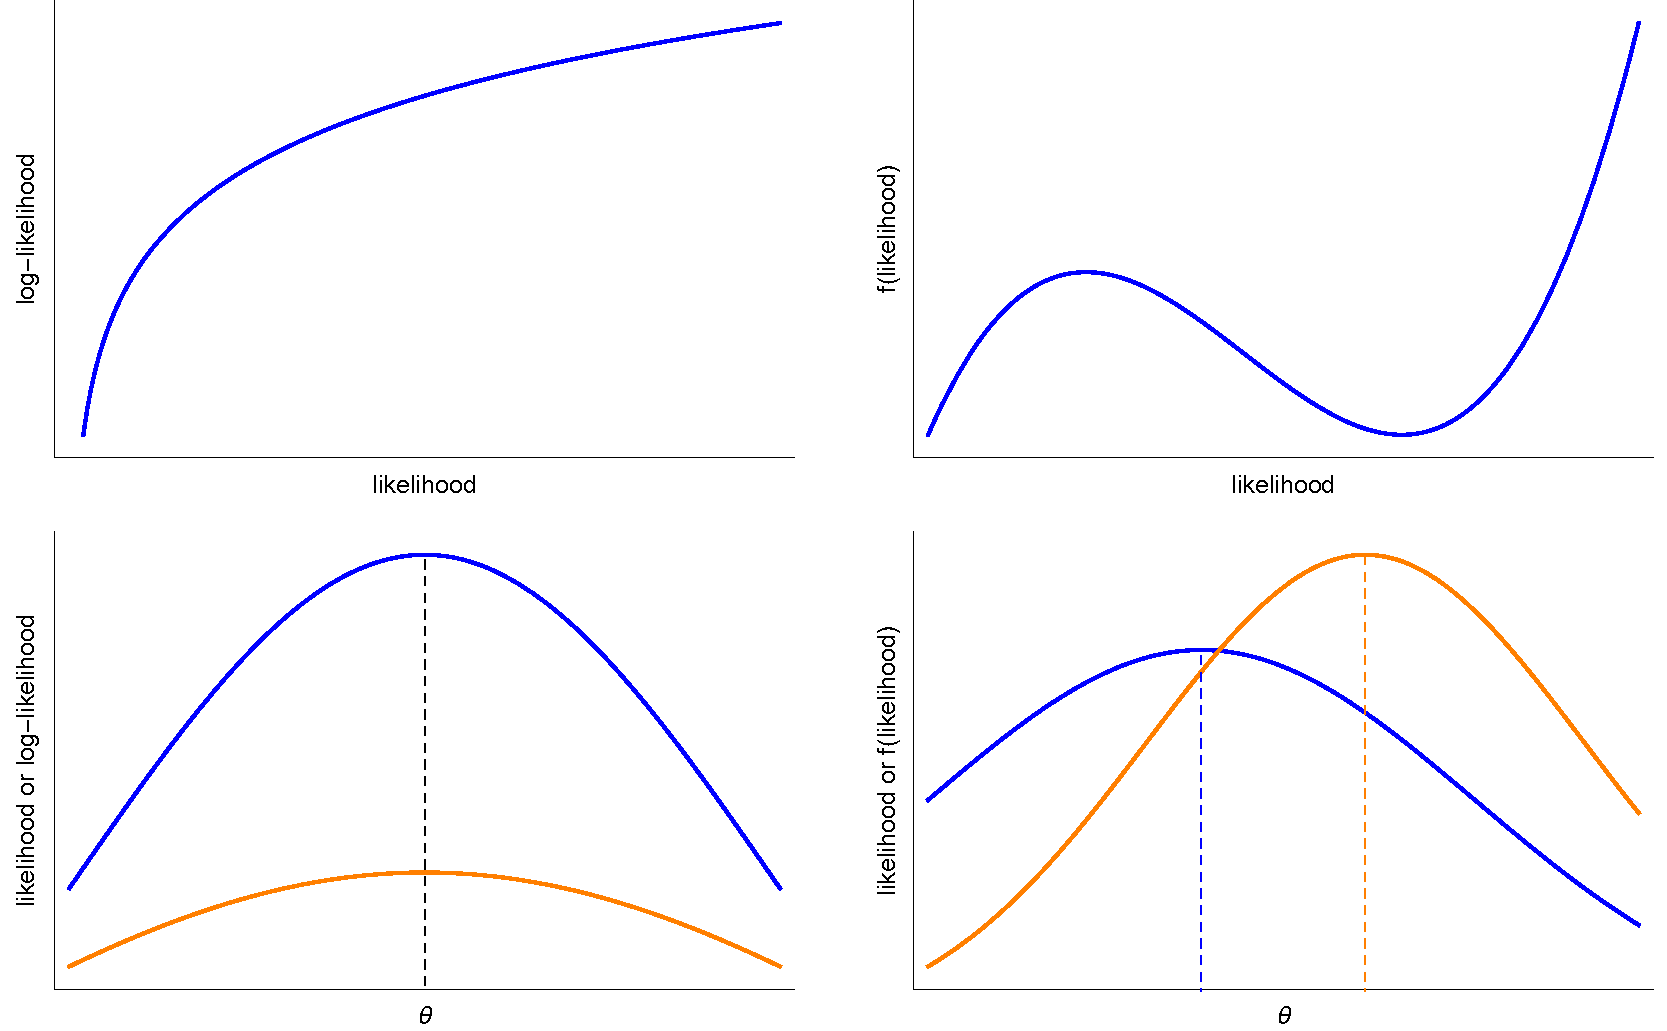
\includegraphics{Likelihood_logMonotonicity.pdf}}
\caption{The monotonicity of log-likelihood (top-left), means that the peaks of likelihood and log-likelihood coincide (bottom-left). However, this is not the case for an arbitrary function (top-right and bottom-right).\textbf{Add legends to the bottom two graphs.} }\label{fig:Likelihood_logMonotonicity}
\end{figure}

Remember, that since we are varying $\theta$ and holding the data constant here, that (\ref{eq:Likelihood_binomialNew}) is a \textit{likelihood}, not a probability. We then need to simply choose $\theta$ so that we can maximise the likelihood. We could simply differentiate (\ref{eq:Likelihood_binomialNew}) as it stands, and set the derivative equal to 0; rearranging the resultant equation for $\theta$. However, to make life a little easier for us, we are first going to take the \textit{log} of this expression, then differentiate it, setting the derivative to 0; resulting in the same value of $\theta$. We are able to do this because of the simple properties of the log transformation (see figure \ref{fig:Likelihood_logMonotonicity}):

\begin{equation}\label{eq:Likelihood_logLikelihoodBinomial}
l(\theta|data) = Log \left(L(\theta|data)\right) = log{100 \choose 10}+ 10log(\theta)+ 90 log(1-\theta)
\end{equation}

Where to get the result (\ref{eq:Likelihood_logLikelihoodBinomial}), we have used the log rules:

\begin{equation}\label{eq:Likelihood_logRules}
\begin{align}
log(ab) &= log(a) + log(b)\\
log(a^b) &= blog(a)
\end{align}
\end{equation}

We can now simply differentiate the log-likelihood $l(\theta|data)$:

\begin{equation}\label{eq:Likelihood_binomialderiv}
\frac{\partial l}{\partial \theta} = \frac{10}{\hat{\theta}}-\frac{90}{1-\hat{\theta}} = 0
\end{equation}

If we set the derivative to 0 we then obtain the maximum likelihood \textit{estimate}, $\hat{\theta} = \frac{1}{10}$ (see figure \ref{fig:Likelihood_MLE}).

\begin{figure}
\centering
\scalebox{0.75} 
{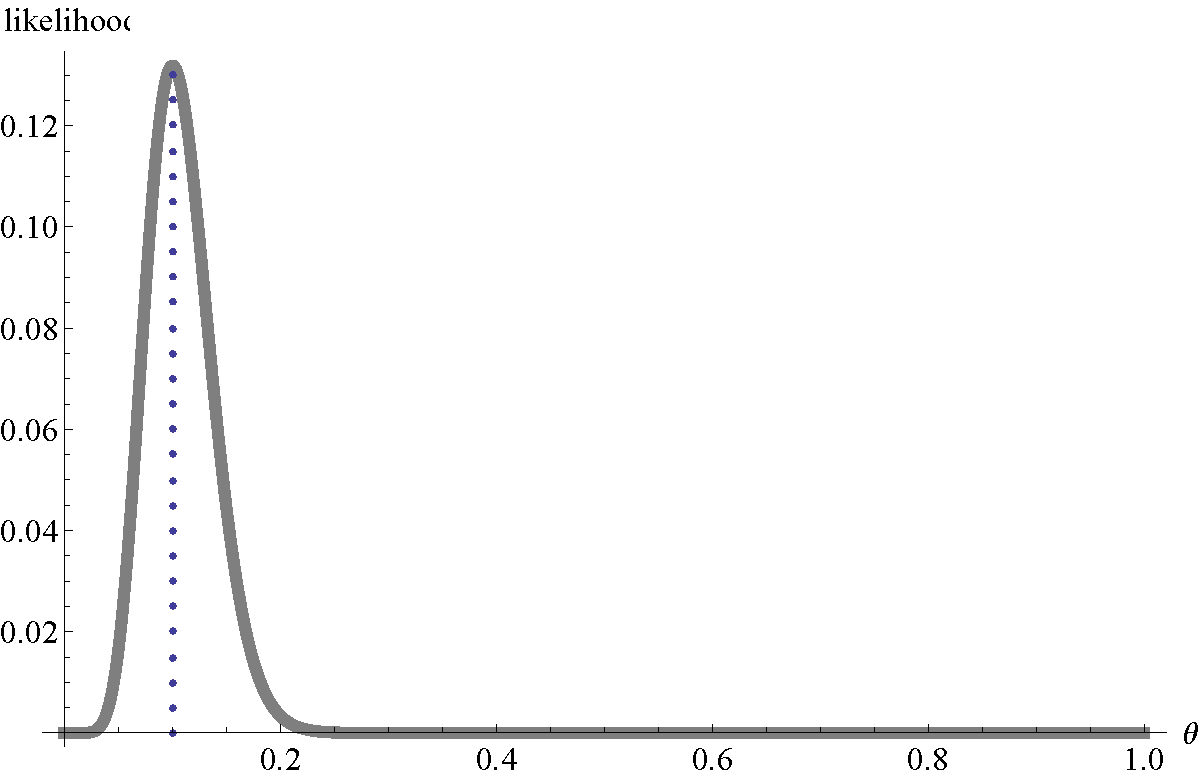
\includegraphics{Likelihood_ML.pdf}}
\caption{Log-likelihood of disease prevalence from section \ref{sec:Likelihood_diseaseMLE} as a function of the proportion of individuals which have the disease in a population, $\theta$. The dotted line shows the maximum likelihood estimate $\hat{\theta}=1/10$.}\label{fig:Likelihood_MLE}
\end{figure}


This estimator makes sense intuitively. The value of the parameter which results in the highest likelihood of obtaining the data occurs when the population prevalence exactly matches that obtained in our sample. In general if we found a number $\beta$ of individuals out of a sample of size $N$, who were disease-positive, then we would again find that the preceding analysis results in an estimator\footnote{An estimator is a mathematical function which outputs an estimate of a parameter in our model.} of the disease prevalence exactly equal to that in our sample:

\begin{equation}\label{eq:Likelihood_binomialestimator}
\hat{\theta} = \frac{\beta}{N}
\end{equation}

\subsection{Estimating the mean and variance in intelligence scores}
We are given a sample of individuals with test scores $\{75,71\}$, and we model the test scores using a normal likelihood as described in section \ref{sec:Likelihood_normal}:

\begin{equation}\label{eq:Likelihood_normalTwo}
L(\mu,\sigma^2|X_1=75,X_2 =71) = \frac{1}{\sqrt{2\pi\sigma^2}}e^{-\frac{(75-\mu)^2}{2\sigma^2}}\times \frac{1}{\sqrt{2\pi\sigma^2}}e^{-\frac{(71-\mu)^2}{2\sigma^2}}
\end{equation}

We can then proceed as we did in section \ref{sec:Likelihood_diseaseMLE} by taking the log of this expression before we differentiate it:

\begin{equation}\label{eq:Likelihood_diseaseLogLikelihood}
l(\mu,\sigma^2|X_1=75,X_2 =71) = 2log\left(\frac{1}{\sqrt{2\pi\sigma^2}}\right)-{\frac{(75-\mu)^2}{2\sigma^2}}-{\frac{(71-\mu)^2}{2\sigma^2}}
\end{equation}

Where we have again used the log rules in (\ref{eq:Likelihood_logRules}) to achieve (\ref{eq:Likelihood_diseaseLogLikelihood}). We can now proceed to differentiate (\ref{eq:Likelihood_diseaseLogLikelihood}) with respect to both variables, holding the other constant, setting each to 0:

\begin{equation}\label{eq:Likelihood_diseaseDerivativeOne}
\begin{align}
\frac{\partial l}{\partial \mu} &= {\frac{(75-\hat{\mu})}{\hat{\sigma^2}}}+{\frac{(71-\hat{\mu})}{\hat{\sigma^2}}} = 0\\
\frac{\partial l}{\partial \sigma^2} &= -\frac{1}{\hat{\sigma^2}} + \frac{(75-\hat{\mu})^2+(71-\hat{\mu})^2}{2\hat{\sigma^4}} = 0
\end{align}
\end{equation}

The first of these expressions yields $\hat{\mu} = \frac{71+75}{2} = 73$, which when put into the second gives: 

\begin{equation}
\hat{\sigma^2} = \frac{1}{2}\left[(75-73)^2 + (71-73)^2)\right] = 4
\end{equation}

Notice that the maximum likelihood estimators for the population mean and variance are for this case the \textit{sample mean} and \textit{sample variance}\footnote{Albeit a biased estimator of the population variance. The unbiased estimator would divide by 1, rather than 2.}. In fact, this holds for the case of N individuals' data, then the maximum likelihood estimators for this case would be:

\begin{equation}
\hat{\mu} = \frac{1}{N}\sum\limits_{i=1}^{N} X_i = \bar{X}
\end{equation}
\begin{equation}
\hat{\sigma^2} = \frac{1}{N}\sum\limits_{i=1}^{N}(X_i-\bar{X})^2 = s^2
\end{equation}

\section{Frequentist inference in Maximum Likelihood}
We have now detailed how to derive point estimates of parameters using the method of maximum likelihood. However, at the moment we are unable to make any conclusions about the population. This is because we do not have any idea as to whether we obtained a particular estimate of a parameter due to picking a weird sample, or because it \textit{actually} has a value in the population which is at this value. Frequentists get round this by examining a graph of log-likelihood near the maximum likelihood point estimate (see figure \ref{fig:Likelihood_likelihoodCurvature}). If the log-likelihood is strongly peaked near the maximum likelihood estimate, then this suggests that only a small range of parameters would yield a similar valued likelihood. By contrast, if the log-likelihood is gently peaked near the ML estimate, then it is feasible that a large range of parameters would yield estimates close to this value. In the latter case, it seems logical that we should be less confident in the particular value of the parameter which is given by maximum likelihood. We can measure the 'peakedness' in the log-likelihood by looking at the magnitude of the second derivative\footnote{The first derivative gives the gradient, the second derivative gives the rate of change of the gradient - a measure of curvature.} of the function at the ML point estimate value. The more curved the log-likelihood, the more confident we can be of our estimated parameter value, and any conclusions drawn from this. Note however, that the Frequentist inference is not based on proper probability distributions (since we infer based on a likelihood). This contrasts with the Bayesian method which, by its nature, allows for a more adequate description of parameters, using probability distributions.

\begin{figure}
\centering
\scalebox{0.65} 
{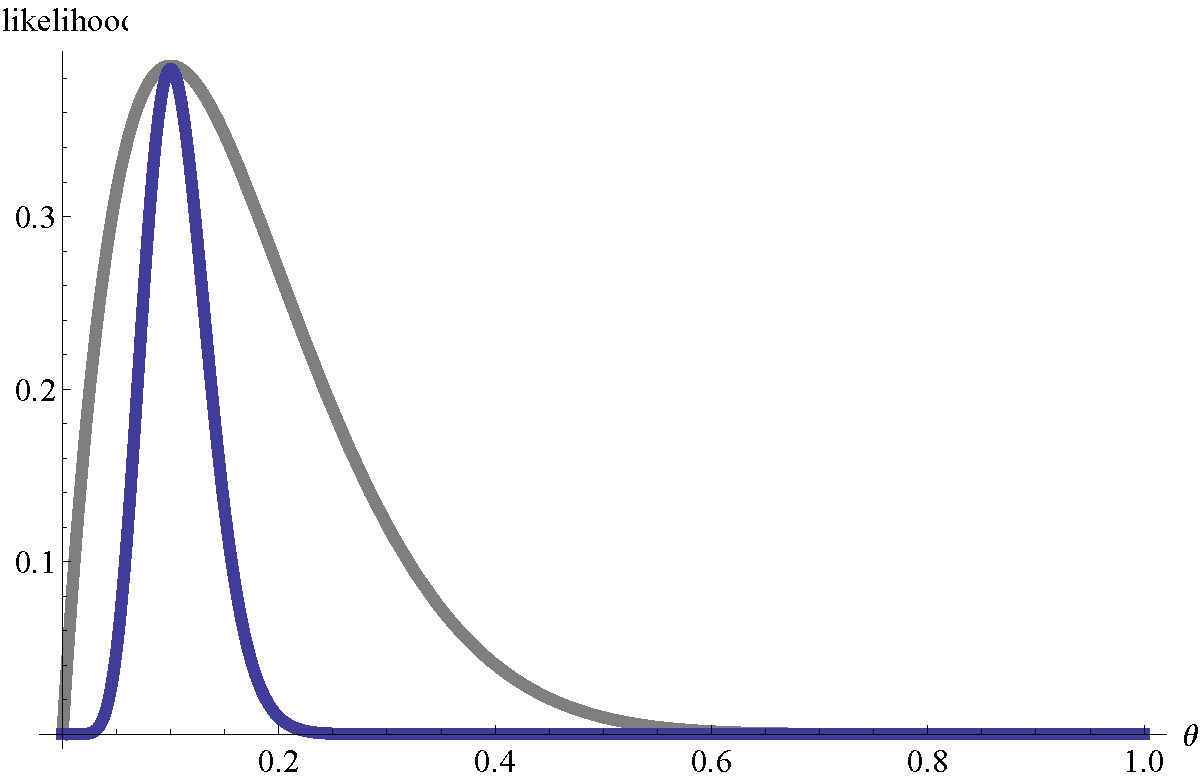
\includegraphics{Likelihood_likelihoodCurvature.pdf}}
\caption{Two likelihoods which result in the same maximum likelihood estimates of parameters, at 0.1. The gray likelihood is less strongly-peaked, meaning we can be less confident about the estimates.}\label{fig:Likelihood_likelihoodCurvature}
\end{figure}


\section{Chapter summary}
We should now understand what is meant by a likelihood, and how to build probabilistic models of real life processes. However, the difficulty of modelling a process is governed by its degree of complexity and sensitivity to violations of assumptions. Further we should also understand how the Frequentist method of Maximum Likelihood can be used to yield point estimates of parameters. We are however, currently restricted in our ability to make inferences based on full probability distributions over parameters. Bayes' rule tells us how we can convert a likelihood - itself not a proper probability distribution - to a posterior (\textit{correct}) probability distribution for parameters. In order to use to do this though, we need to understand what is meant by a \textit{prior} distribution and how we can specify this distribution to suit the particular situation. This is what is covered in the next chapter.

\section{Chapter outcomes}
The reader should now be familiar with the following concepts:

\begin{enumerate}
\item The difference between likelihoods and probabilities.
\item The need for probabilistic models in some circumstances.
\item How to go about choosing an appropriate likelihood for a given situation.
\item The exchangeability assumption.
\item Maximum likelihood, and how to carry out inference in this framework.
\end{enumerate}

\section{Problem set}
\subsection{Blog blues.}
We suppose that visits to your newly-launched blog occur sporadically. Suppose you were interested in the length of time between consecutive first-time visits to your homepage. You collect the time data for a given 100 visits to your blog for a particular time period and day, and you set about thinking about building a statistical model.
\subsubsection{What assumptions might you make about the first-time visits?}
\subsubsection{What model might be appropriate to model the time between visits?}
\subsubsection{Algebraically derive an estimate of the mean number of visits per hour}
\subsubsection{Data analysis:} you collect time data from Google Analytics\footnote{A popular provider of website analytics data.} for 1000 visits. The data set is called XXXX. \textbf{Derive an estimate of the mean number of visits per hour.}
\subsubsection{Graph the log likelihood near your estimated value. What does this show? Why don't we plot the likelihood?}
\subsubsection{Estimate confidence intervals around your parameter.}
\subsubsection{What is the probability that you will wait:}
\begin{enumerate}
\item 1 minutes or more.
\item 5 minutes or more.
\item Half an hour or more.
\end{enumerate}
before your next visit?
\subsubsection{Evaluate your model.}
\subsubsection{What alternative models might be useful here?}
\subsubsection{What are the assumptions behind these models?}
\subsubsection{Estimate the parameters of your new model.}
\subsubsection{Use your new model to estimate the probability that you will wait:}
\begin{enumerate}
\item 5 minutes.
\item 20 minutes.
\item 1 hour.
\end{enumerate}
before your next visit?

\subsubsection{Hints: the exponential is to the poisson model, what the ? is to the negative binomial.}

\subsection{Violent crime counts in New York counties}
In data file XXX we have compiled a data set of the population, violent crime count and unemployment across New York counties in 2014. 

\subsubsection{Graph the violent crime account against population. What type of relationship does this suggest?}
\subsubsection{A simple model}
A simple model here might be to assume that the crime count in a particular county is related to the population size by a poisson model:
\begin{equation}
crime_i \sim poisson(n_i\theta)
\end{equation}
\subsubsection{What are the assumptions of this model?}
\subsubsection{Estimate the parameter $\theta$ from the data. What does this parameter represent?}
\subsubsection{Do these assumptions seem realistic?}
\subsubsection{Estimate a measure of uncertainty in your estimates.}
\subsubsection{Evaluate the performance of your model.}

\subsubsection{A better model}
An alternative model allows each county to be heterogeneous with respect to its susceptibility to crime, and has a specification of the form:
\begin{equation}
crime_i \sim poisson(n_i\theta_i)
\end{equation}
\subsubsection{Why is this model better?}
\subsubsection{What factors might affect $\theta_i$?}
\subsubsection{Write down a new model specification taking into account the previous point.}
\subsubsection{Estimate the parameters of this new specification.}
\subsubsection{How does this new model compare to the previous iteration?}
\subsubsection{What alternative specifications might be worth attempting?}

\subsection{Monte Carlo evaluation of the performance of MLE in R}
Ben to add later.

\subsection{The sample mean as MLE}
Ben to add later.

\chapter{Priors}\label{chap:Prior}
\section{Chapter Mission statement}
At the end of this chapter a reader will know what is meant by a prior, and the different philosophies that are used to understand and construct them. 

Insert a graphic with the likelihood part of Bayes' formula circled, as in the equation shown below for the part highlighted in blue.

\begin{equation}
p(\theta|data) = \frac{p(data|\theta)\times {\color{blue}p(\theta)}}{p(data)}
\end{equation}\label{eq:Prior_BayesHighlighted}

\section{Chapter goals}
Bayes' rule tells us how to convert a likelihood - itself not a proper probability distribution - into a posterior probability distribution for parameters, which can then be used for inference. We are required in the numerator to multiply the likelihood by a pre-experimental weighting of each set of parameter values described by a probability distribution, which is known as a \textit{prior}. Priors are without doubt the most controversial aspect of Bayesian statistics, with opponents criticising its inherent \textit{subjectivity}. It is hoped that by the end of the chapter we will have convinced the reader that, not only is subjectivity inherent in \textit{all} statistical models - both Frequentist and Bayesian - but the explicit subjectivity of priors is more transparent, and hence open to interrogation, than the implicit subjectivity abound elsewhere.

This chapter will also explain the differing interpretations which are ascribed to priors. The reader will come to understand the types of method that can be used to construct prior distributions, and how they can be chosen to be minimally subjective, or otherwise to contain informative pre-experimental insights from data or opinion. Finally, the reader will understand that if significant data are available then the conclusions drawn should be insensitive to the initial choice of prior.

Inevitably, this chapter will be slightly more philosophical and abstract than other parts of this book, but it is hoped that the examples given will be sufficient to ensure its practical use.

\section{What are priors, and what do they represent?}
Chapter \ref{chap:Likelihoods} introduced us to the concept of formulating a likelihood, and how this can be used to derive Frequentist estimates of parameters, using the method of maximum likelihood. This pre-supposes that the parameters in question are immutable, fixed quantities that actually exist, and can be estimated by methods that can be repeated, or imagined to be repeated many times \cite{gill2007bayesian}. As Gill (2007) indicates, this is unrealistic for the vast majority of social science research.

\begin{quotation}
It is simply not possible to rerun elections, repeat surveys under exactly the same conditions, replay the stock market with exactly matching market forces, or re-expose clinical subjects to identical stimuli.
\end{quotation}

Furthermore, parameters only exist because we have \textit{invented} a model, hence we should innately be suspicious of any analysis which assumes an existence of a single certain value for any aspect of these abstractions.

For Bayesians, it is the data that are treated as fixed, and the parameters that vary. We know that the likelhood - however useful - is not a proper probability distribution. Bayes' rule tells us how to combine a likelihood with something called a \textit{prior} to obtain a proper posterior distribution for the parameter in question, which can then be used for inference. But what does it actually mean for a parameter to have a prior distribution?

Gelman et al. (2013) suggests that there are two different interpretations of priors: the \textit{state of knowledge} interpretation, where we specify our knowledge and uncertainty in a parameter as if regarding it as a draw from a probability distribution; alternatively in the more objective \textit{population} interpretation where the current value of a parameter is the result of a draw from a true population distribution \cite{gelman2013bayesian}. In both viewpoints the model parameters are not viewed as static, unwavering constants as they are taken to be in Frequentist theory.

\begin{figure}
\centering
\scalebox{0.3} 
{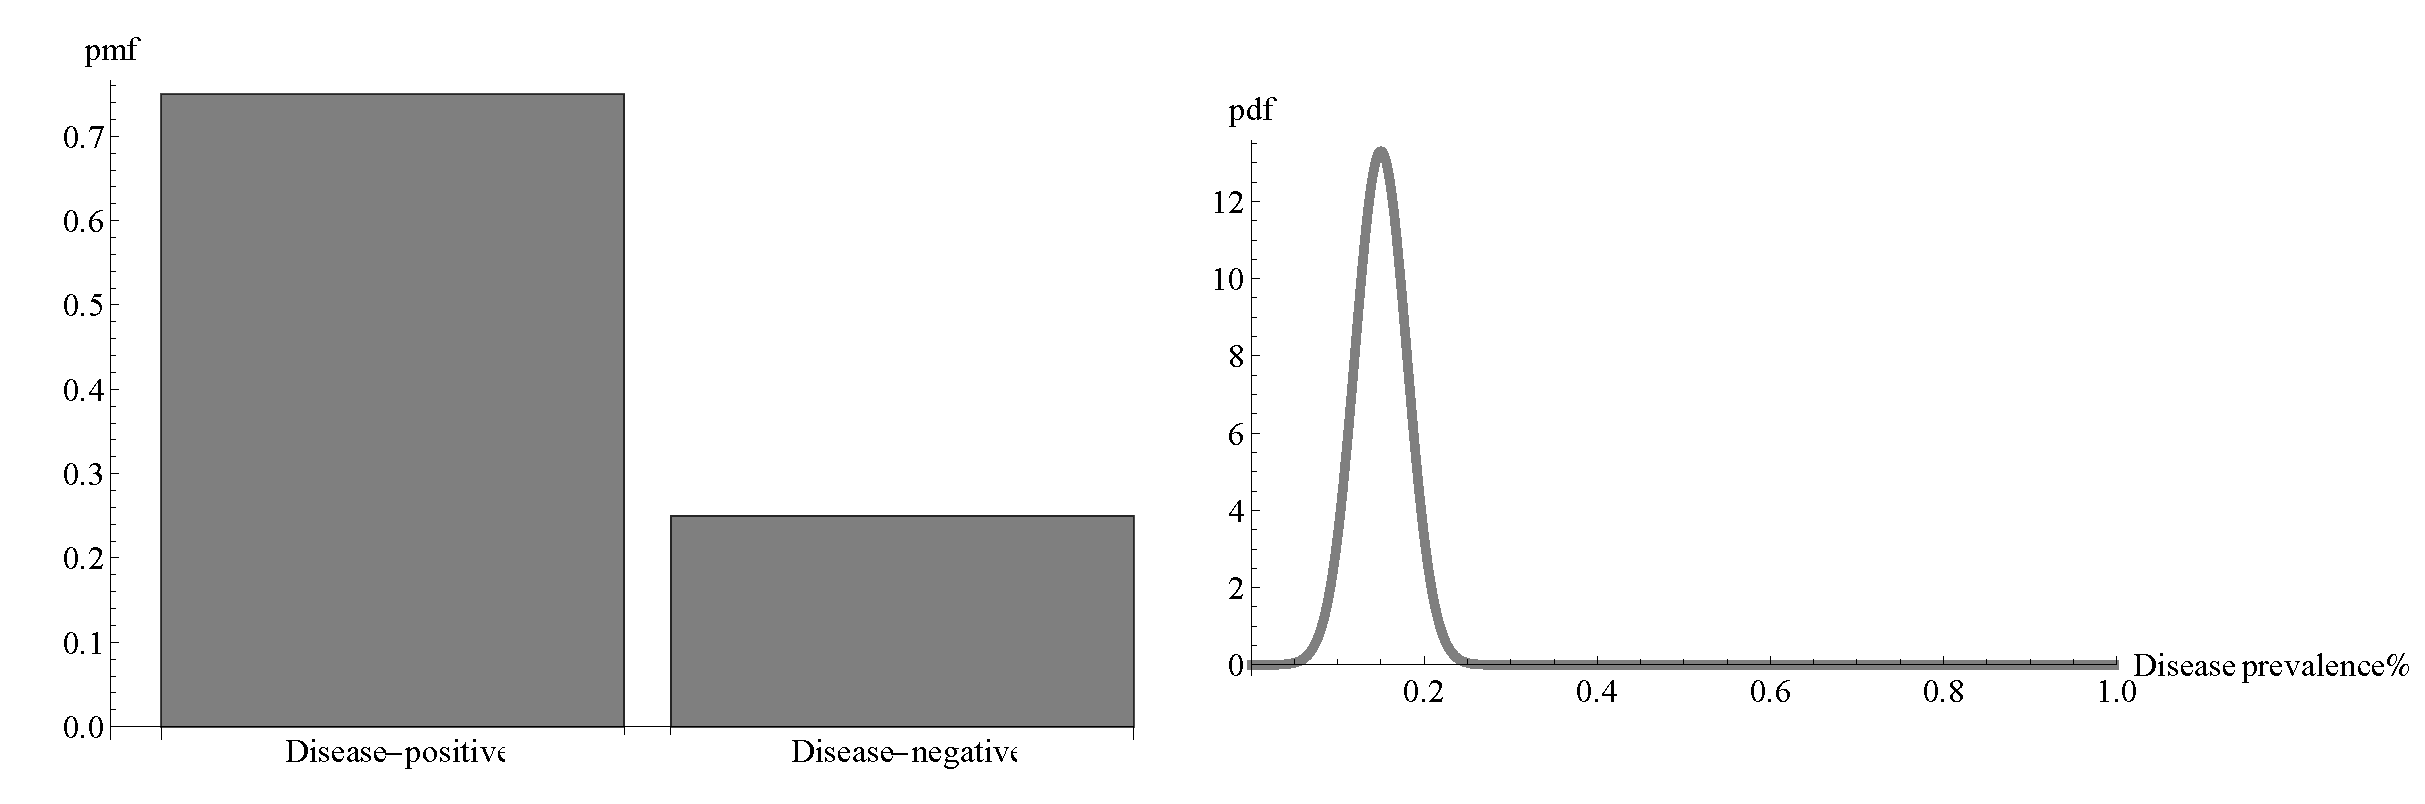
\includegraphics{Prior_introduction.pdf}}
\caption{Left - a prior for a doctor's pre-testing diagnostic probability of an individual having a disease. Right - a prior which represents pre-sample uncertainty in disease prevalence.}\label{fig:Prior_introduction}
\end{figure}

If we adopt the \textit{subjective} state of knowledge viewpoint above, then we can think of the prior as representing our pre-experimental/data certainty in the parameter in question. For example, imagine that a Doctor is asked to evaluate the probability that a given individual has a particular disease, before the results of a blood test become available. Using their knowledge of the patient's history and their expertise on the particular condition, they assign a prior disease probability of 75\% (see figure \ref{fig:Prior_introduction}). 

Alternatively, imagine we are tasked with estimating the proportion of the UK population that has this disease. We may have some idea of its prevalence, as well as the variance in the mean prevalence of a disease across a range of previous samples of individuals which have been tested. In this case, the prior is continuous and represents our uncertainty in our estimate of the prevalence (see figure \ref{fig:Prior_introduction}). 

In all cases a prior is a proper probability distribution, and hence can be used to elicit our prior expectations as to the value of a parameter. For example, we could use the prior probability distribution for the proportion of individuals having a particular disorder in figure \ref{fig:Prior_introduction} to estimate a pre-experimental mean of approximately 15\% prevalence. 

Adopting the \textit{population} perspective, we imagine the value of a parameter of current interest to be drawn from a population distribution. If we imagine the process of flipping a coin, we could if we knew the angle at which it is tossed, as well as the height from which it is thrown above the surface\footnote{Also assuming that we knew the physical properties of the coin and surface.} predict deterministically the side on which the coin would fall face up. We could then hypothetically enumerate the (infinitely) many angles and heights of the coin, and for each set determine whether the coin would fall face up or down. Each time we throw the coin we are implicitly choosing an angle and height from the set of all possible combinations, which determines whether a heads or tails falls face up. Some ranges of the angle and the height will be more frequently chosen than others, albeit relatively agnostic with regards to final state of the coin.  Hence we could think of this choice as the realisation from a distribution of all possible sets. Thus we could think about the choice of angle and height as being a realisation from this \textit{population} distribution, and hence determines the fate of the coin toss.

\boxed{Interactive:} see the interactive tool XXX which allows you to investigate the population interpretation of priors for local literacy rates in the US. 

Alternatively, going back to the disease prevalence example, we could imagine that each time we pick a sample, the data we obtain is partly determined by the exact characteristics of the sub-populations from which these individuals were drawn. The other part of variability is sampling variation within those sub-populations. Here we can view the particular sub-population characteristics as draws from an overall population distribution of parameters, representing the entirety of the UK. 

\section{Why do we need priors at all?}
A question we might ask is, why do we need priors at all? Can't we simply let the data speak for itself, without the need of these subjective beasts? 

Frequentists without knowing it actually do use something equivalent to priors, by setting the size of statistical tests\footnote{See section \ref{sec:Intro_implicitExplicitSubjectivity} for a further discussion.}. However, can't we as Bayesians side-step this subjective jump completely?

The answer to this question is provided by Bayes' rule. Its inclusion in Bayes' rule, which is the only correct way to update beliefs, means that if we are to be consistent with the laws of probability, we are required to provide this part for any Bayesian inferential procedure. 

If you find this description somewhat unsatisfying, then another way of re-phrasing this argument, is that Bayes' rule is really only a way to \textit{update} our initial beliefs, to yield new beliefs which reflect the weight of the data obtained:

\begin{equation}
initial\; belief \xrightarrow{Bayes' rule} new\;beliefs
\end{equation}

Viewed in this light, it is clear that we need to specify an initial belief, otherwise we have nothing to update! Bayes unfortunately doesn't tell us how to formulate this initial belief, but fear not, in this chapter we will delve into how we can go about setting priors in practice.

\section{Why don't we just normalise likelihood by choosing a unity prior?}\label{sec:Prior_unityPrior}
Another question that can be asked is, 'Why can't we simply let the prior be the same for all values of $\theta$?'; in other words set $p(\theta) = 1$ in the numerator of Bayes' rule; resulting in a posterior that takes the form of a normalised likelihood:

\begin{equation}
p(\theta|data) = \frac{p(data|\theta)} {p(data)}
\end{equation}\label{eq:Prior_BayesNormalisedLikelihood}


This would surely negate the need for specification of a prior, and thwart all attempts to denounce Bayesian statistics as \textit{subjective}. So why don't we do just that? 

There is a pedantic, mathematical argument against this, which is that $p(\theta)$ must be a proper probability distribution to ensure the same properness of the posterior. If we choose $p(\theta) = 1$ (or in fact any positive constant), then the integral $\int\limits_{-\infty}^{+\infty}p(\theta)\mathrm{d}\theta\rightarrow\infty$, and we can no longer think of the distribution, $p(\theta)$ as representing a probability distribution. It may still be possible that even if the prior is improper, that the resultant posterior also satisfies the required properties of a proper probability distribution, but care must be taken when using these distributions for inference, as technically they are \textit{not} probability distributions, due to the abuse of Bayes' rule. In this case the posteriors can only be viewed, at best, as approximations to the result we would have obtained under some limiting prior distribution.

Another, perhaps more persuasive argument, is that by assuming all parameter sets have an equal likelihood of being chosen beforehand, then this can result in nonsensical resultant conclusions being drawn. Consider the following example: 

We are given some data on a coin which has been flipped twice, with the result $\{H,H\}$. We are given the choice of deciding whether the  coin is fair, with an equal chance of both heads and tails occurring, or biased with a very strong weighting towards heads. We denote fairness by a parameter $\theta=1$, if the coin is fair, and $\theta=0$ otherwise.

\begin{figure}
\centering
\scalebox{0.1} 
{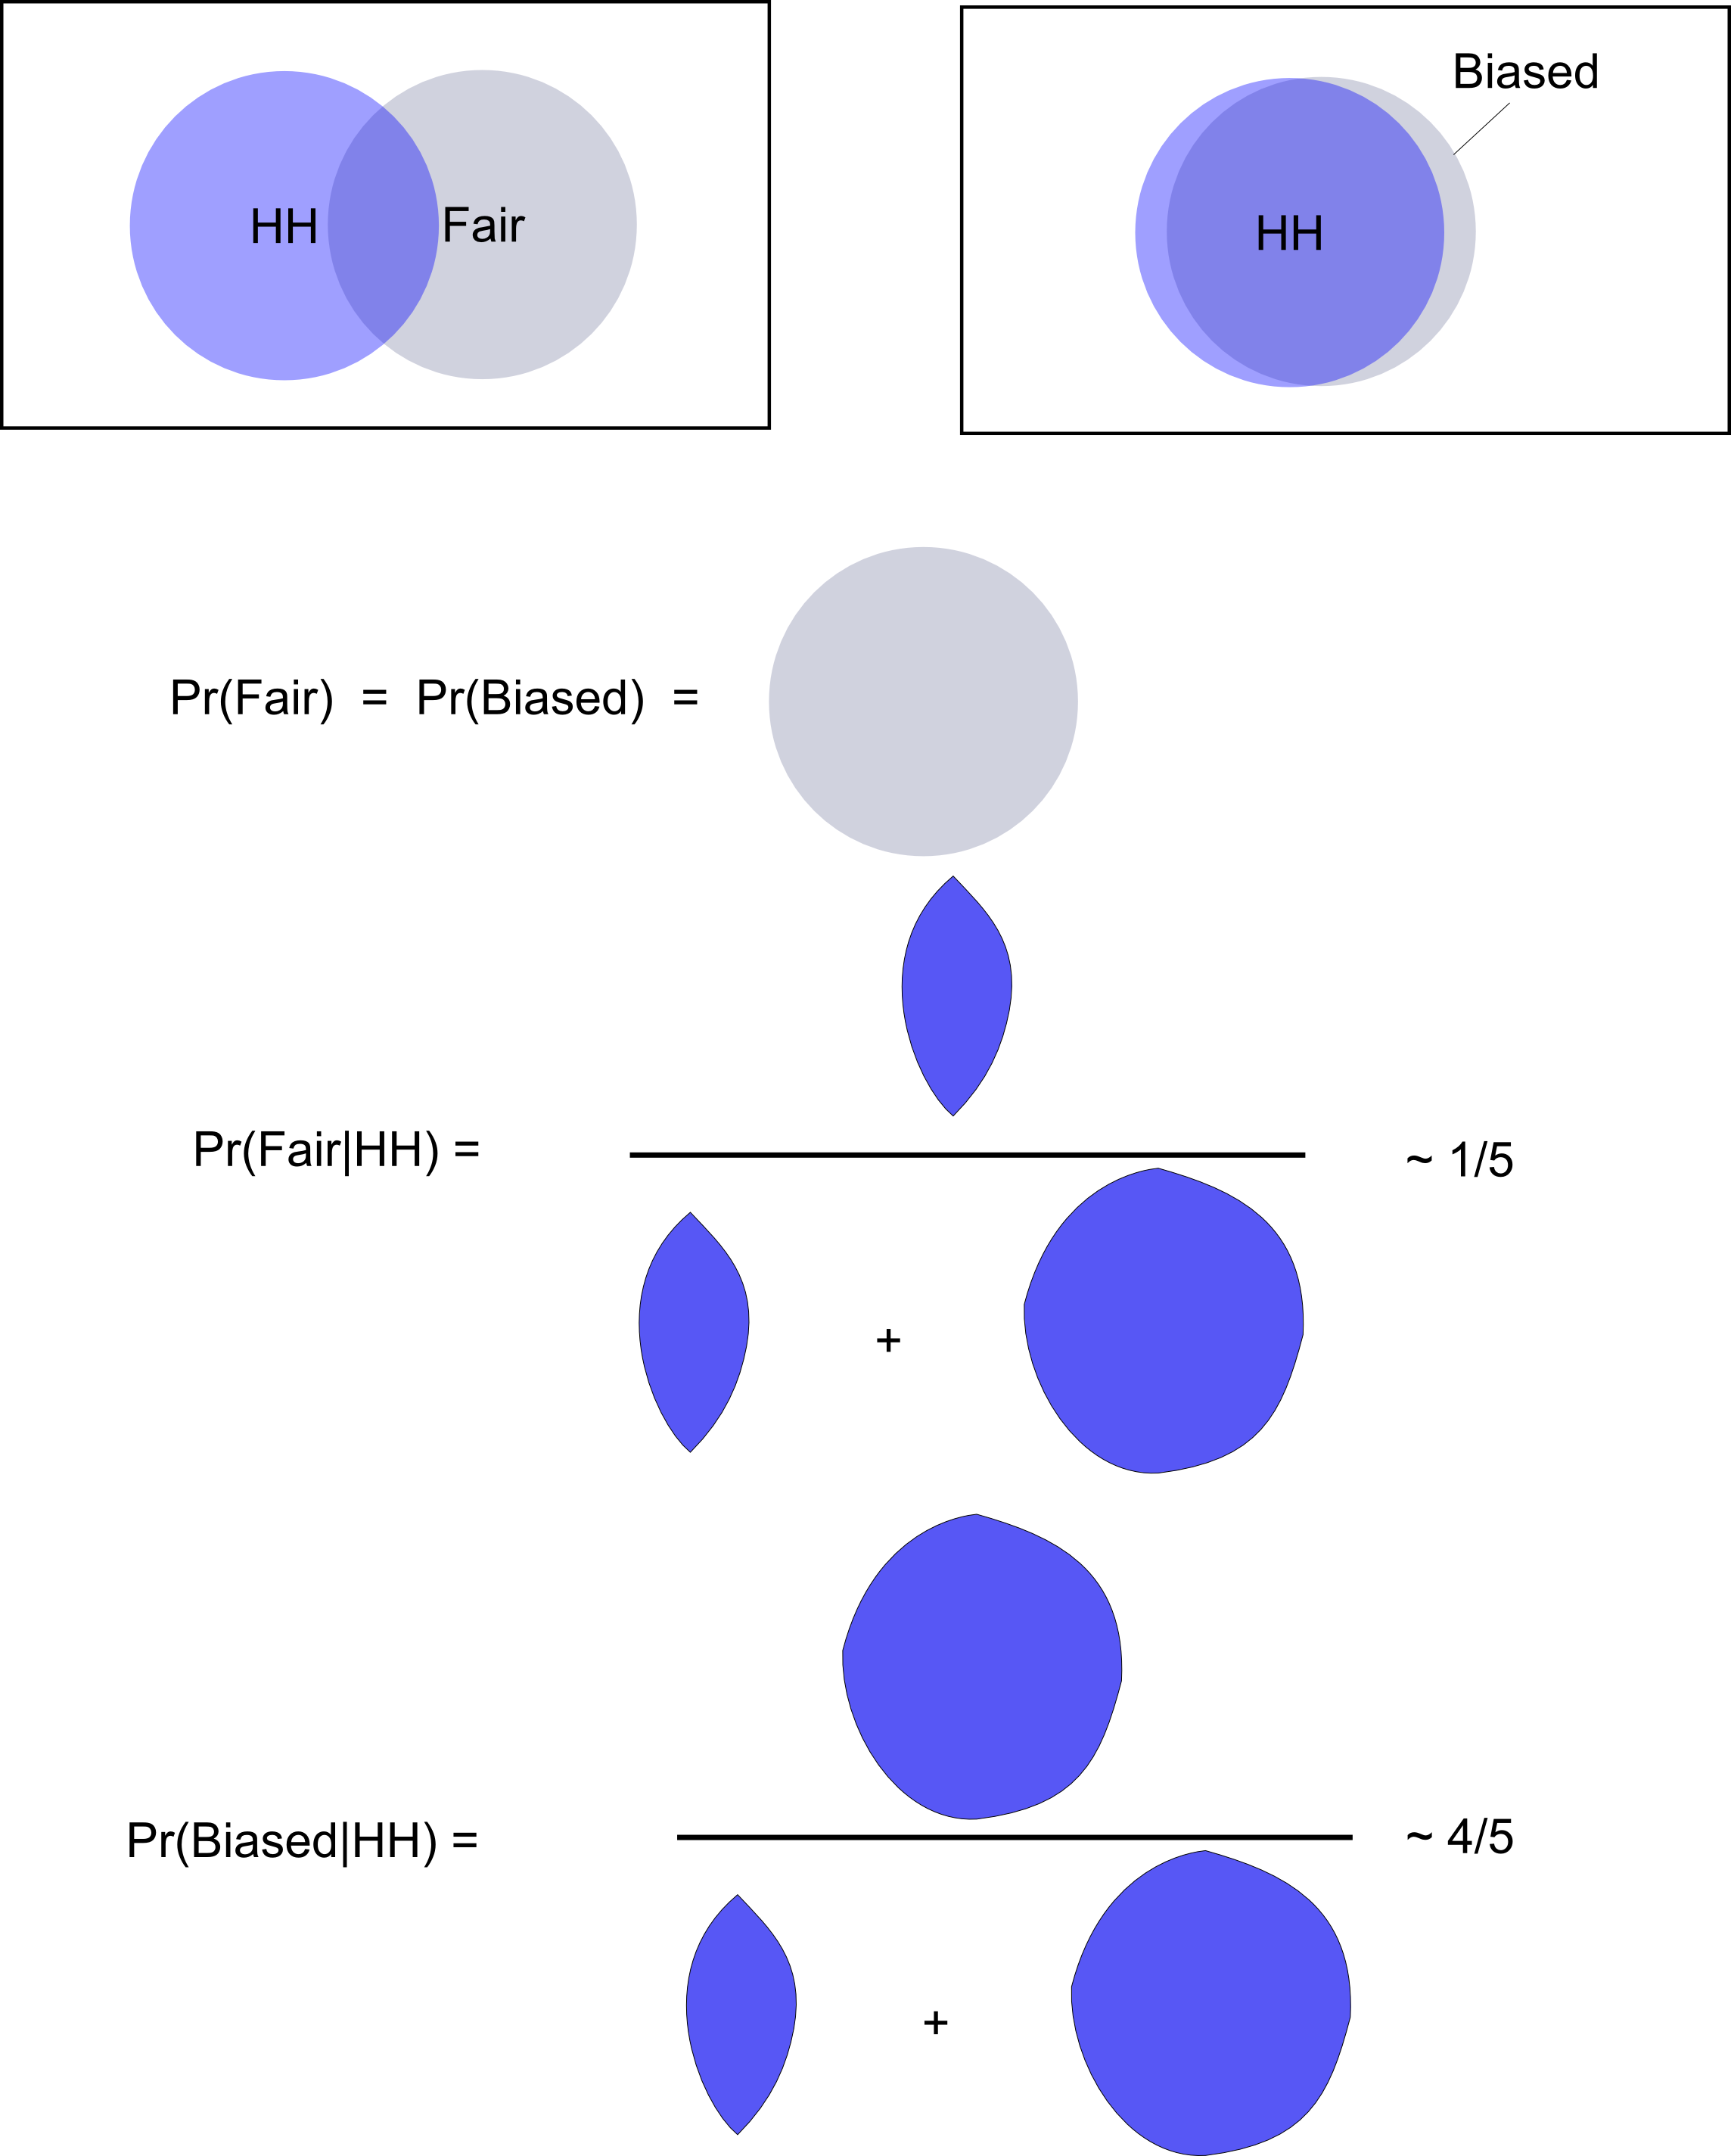
\includegraphics{Prior_priorJustificationCoin.png}}
\caption{Ignoring common sense, by setting a uniform prior between a coin being fair and biased, results in an unrealistic posterior; supposing that the coin is \textit{very} likely to be biased.}\label{fig:Prior_priorJustificationCoin}
\end{figure}

Figure \ref{fig:Prior_priorJustificationCoin} illustrates how assuming a uniform prior in this case results in a very strong posterior weighting towards the coin being biased. This is because from a likelihood perspective - $p(data|\theta)$ - if we assume that the coin is biased, then the probability of obtaining two heads is high. Whereas if we assume that the coin is fair, then the probability of obtaining this data is only $\frac{1}{4}$. Thus, by ignoring common sense - that it is likely the majority of coins are relatively unbiased - we end up with a result that is nonsensical. 

\boxed{Interactive:} see the interactive tool XXX which allows you to play around with your prior probability of a coin being biased, and note its effect on the posterior.

Of course, in this example we would hope that by collecting more data, in this case, throws of the coin, we could be confident in the conclusions drawn from the likelihood. However, Bayesian analysis allows us to achieve such a goal with a smaller sample size, should we be relatively confident about our pre-data knowledge.

\section{The explicit subjectivity of priors}
Opponents of Bayesian approaches to inference criticise the subjectivity inherent with choice of prior. However, all analysis involves a degree of subjectivity, particularly in regard to choice of statistical model. This choice is often formulated implicitly as being \textit{objectively} correct, with little justification or discourse given to the underlying assumptions necessary to arrive there. The statement of a prior, necessary for any full description of a Bayesian analysis, is at least \textit{explicit}; leaving this aspect of the modelling subject to the same interrogation and academic examination to which any analysis should be subjected. A word that is often used by protagonists of Bayesian methods, is that it is \textit{honest} due to the \textit{explicit} statement of assumptions. The statement of pre-experimental biases actually forces the analyst to self-examine, and perhaps also leads to a decline in the temptation to manipulate the analysis to one's own ends.

\section{Combining a prior and likelihood to form a posterior} 
This chapter thus far has given more attention to the philosophical and theoretical underpinnings of Bayesian analysis. Now we change tack to illustrate to the reader the mechanics behind Bayes' formula; specifically how the prior is combined with the likelihood to yield a posterior probability distribution. The following examples introduce an illustrative method, known as \textit{Bayes' box} described in detail in \cite{stewart2014teaching} and \cite{bolstad2007introduction}, which illustrates the functioning of Bayes' rule, in which the parameter, prior, likelihood, and posterior are all displayed in a logical manner.

\subsection{The Goldfish game}\label{sec:Prior_urn}
Imagine a covered bowl of water, containing 5 fish, each of which is red or white, and suppose we are tasked with inferring the total number of red fish which are present in the bowl, on the basis of a single fish which we pick out, and find to be red. Before we pull the fish out from the bowl, we have no prejudice for a particular number of red fish, and so suppose that all possibilities - 0 to 5 - are equally likely, and hence have the probability of $\frac{1}{6}$ in our discrete prior. Our model for the likelihood is that a number $Y$ of the fish are red, and that the result of an individual picking a fish from the bowl tells us nothing about future picks, apart from their joint dependence on $Y$. In this oversimplified example, this independence assumption seems reasonable, particularly if the fish are picked out in a randomised manner and have no distinguishing features. Further suppose that the random variable $X\in\{0,1\}$ indicates whether a fish is white or red respectively.  The analogy with the disease status of an individual described in section \ref{sec:Likelihood_individualDisease} is evident, and hence we choose a likelihood of picking a red fish of the form:

\begin{equation}\label{eq:Prior_bernoulli}
P(X = 1|Y=\alpha) = \frac{\alpha}{5}
\end{equation}

In (\ref{eq:Prior_bernoulli}), $\alpha\in\{0,1,2,3,4,5\}$ represents the number of red fish in the bowl.

We can then illustrate the functioning of Bayes' rule in the \textit{Bayes' box} shown in table \ref{tab:Prior_bayesBoxDiscreteUrns}. We start by listing all the possible numbers of red fish that can exist in the bowl in the leftmost column. We then introduce our prior probabilities that we associate with each of the six potential numbers of red fish that can be in the bowl. In the third column we then calculate the likelihoods for each of the outcomes using the simple rule given in (\ref{eq:Prior_bernoulli}). We then multiply the prior by the likelihood in the fourth column, which on summation gives us $p(data)=\frac{1}{2}$, which we use to create a proper probability distribution for the posterior in the last column. For a mathematical description of this process see section \ref{app:Prior_bayesUrn}.

The Bayes' box illustrates the straightforward and mechanical working of Bayes' rule for the case of discrete data. We also note that when we sum the likelihood over all possible numbers of red fish in the bowl - in this case the parameter which we are trying to infer - we find that this to be equal to 3; illustrating again that a likelihood is not a valid probability distribution. We also see that at a particular parameter value, if either the prior or the likelihood are found to be zero as is the case of 0 red fish being in the urn (impossible since we have at least one), then this ensures that the posterior distribution is zero at this point. This makes it important that we use a prior that gives a positive weight to \textit{all} possible ranges of parameter values. The results are also displayed graphically in figure \ref{fig:Prior_urnStacked}.

\begin{table}[htbp]
  \centering
  \caption{A Bayes' box showing how to calculate the posterior for the case of drawing fish from a bowl containing a 5 fish mixture of red and white fish, one of which has been drawn and shown to be red. Here we assume that pre-experiment all possible numbers of red fish are equally likely, by adopting a uniform prior.}\label{tab:Prior_bayesBoxDiscreteUrns}
    \begin{tabular}{ccccc}
    \toprule
    \textbf{Number of red fish} & \textbf{Prior} & \textbf{Likelihood} & \textbf{Prior x likelihood} & \textbf{Posterior$=\frac{Prior\times Likelihood}{p(data)}$} \\
    \midrule
    0     &  1/6  & 0     & 0       & 0       \\
    1     &  1/6  &  1/5  &   1/30 &   1/15 \\
    2     &  1/6  &  2/5  &   1/15 &   2/15 \\
    3     &  1/6  &  3/5  &   1/10 &   3/15  \\
    4     &  1/6  &  4/5  &   2/15 &   4/15 \\
    5     &  1/6  & 1     &   1/6  &   5/15  \\
    \bottomrule
    Total & \textbf{1    } & \textbf{3    } & \textbf{$p(data)=1/2$ } & \textbf{1      } \\
    \bottomrule
    \end{tabular}%
  \label{tab:addlabel}%
\end{table}%

\begin{figure}
\centering
\scalebox{0.75} 
{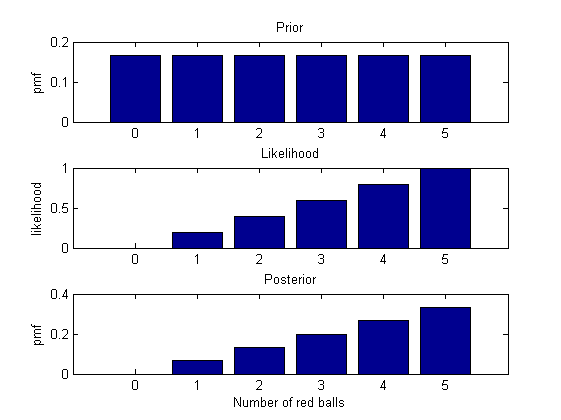
\includegraphics{Prior_urnStacked.png}}
\caption{The prior, likelihood and posterior for the fish example described in \ref{sec:Prior_urn}. The prior in the upper panel gives uniform weighting to all possible numbers of red fish. This is then multiplied by the likelihood (in the middle panel) at each number of fish, and normalised to make the posterior density shown in the bottom panel.}\label{fig:Prior_urnStacked}
\end{figure}

Now suppose that we had reason to believe that the game-maker had a prejudice towards more equal numbers of both fish, and as a result we alter our prior to have a greater weight towards these numbers of red fish(see table \ref{tab:Prior_bayesBoxUrnUpdated} and figure \ref{fig:Prior_bayesUrnUpdated}).


\begin{table}[htbp]
  \centering
  \caption{A Bayes' box showing how to calculate the posterior for the case of drawing fish from a bowl containing a 5 fish mixture of red and white fish, one of which has been drawn and shown to be red. Here we assume that pre-experiment all possible numbers of red fish are equally likely, by adopting a uniform prior.}\label{tab:Prior_bayesBoxUrnUpdated}%
    \begin{tabular}{ccccc}
    \toprule
    \textbf{Number of red fish} & \textbf{Prior} & \textbf{Likelihood} & \textbf{Prior x likelihood} & \textbf{Posterior$=\frac{Prior\times Likelihood}{p(data)}$} \\
    \midrule
    0     &   1/12 & 0     & 0       & 0       \\
    1     &   1/6  &  1/5  &   1/30 &   1/15 \\
    2     &   1/4  &  2/5  &   1/10 &   1/5  \\
    3     &   1/4  &  3/5  &   3/20 &   3/10 \\
    4     &   1/6  &  4/5  &   2/15 &   4/15 \\
    5     &   1/12 & 1     &   1/12 &   1/6  \\
    \bottomrule
    Total & \textbf{1      } & \textbf{3    } & \textbf{  1/2 } & \textbf{1      } \\
    \bottomrule
    \end{tabular}%
  
\end{table}%

\begin{figure}
\centering
\scalebox{0.75} 
{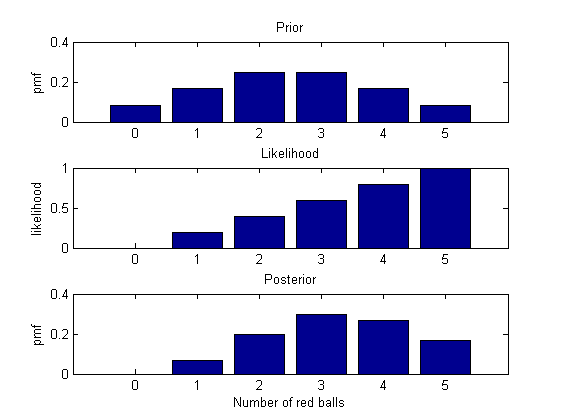
\includegraphics{Prior_bayesUrnUpdated.png}}\caption{The prior, likelihood and posterior for the goldfish game example described in \ref{sec:Prior_urn}. The prior in the upper panel gives more weighting to more equal numbers of red and white fish. This is then multiplied by the likelihood (in the middle panel) at each number of fish, and normalised to make the posterior density shown in the bottom panel.}\label{fig:Prior_bayesUrnUpdated}
\end{figure}


\boxed{Interactive:} see the interactive tool XXX to play the goldfish game!

\subsection{Disease proportions revisited}\label{sec:Prior_diseaseProp}
Suppose that we substitute our goldfish bowl from section \ref{sec:Prior_urn} for a sample of 100 individuals taken from the UK population. Suppose also that we continue to assert the independence of individuals within our sample, and make explicit the assumption that individuals are from the same population, and are hence identically-distributed. We are now interested in making conclusions about the overall proportion of individuals within the population who have the disease, $\theta$. Since the parameter of interest is now continuous, we cannot use Bayes' box as there would be infinitely many rows (corresponding to the continuum of possible $\theta$) over which to sum. Let's suppose that within our sample of 100 we find 3 of them who are disease-positive\footnote{We also suppose that there are no false-positives here.}. We could then use the assumptions of independence and identical-distribution to write down a likelihood of the form introduced in section \ref{sec:Likelihood_diseaseGroup}:

\begin{equation}\label{eq:Prior_binomial}
P(Z=3|\theta) = {100 \choose 3} \theta^\beta (1-\theta)^{100-3}
\end{equation}

The reason for the ${100 \choose 3}=161,700$ term at the beginning of (\ref{eq:Prior_binomial}) is that we have to count the number of different permutations of getting 3 individuals who are disease-positive within a sample size of 100. 

We suppose that at the beginning of the experiment all values of $\theta$ are equally likely. However, we would expect researchers to have a pre-experimental idea as to the most probable frequencies of the disease within the population, meaning that a flat prior which is given is likely understating a prejudice towards a certain range of $\theta$ values. Whilst, this is the case, it is often assumed in research papers - for the sake of objectivity - that priors are flat, in order to try to minimise the effect which assumptions here make on the outcome of an analysis.

The impact of using a flat prior here is that the posterior is peaked at the same value of $\theta$ as the likelihood (see figure \ref{fig:Prior_disease}). 

\subsubsection{Interactive effect of the prior on the posterior}
See the following link to explore the effect of the prior, as well as the data sample, on the posterior for the disease proportions example.


\begin{figure}
\centering
\scalebox{0.75} 
{\includegraphics{Prior_disease.png}}
\caption{The prior, likelihood and posterior for the disease proportion example described in section \ref{sec:Prior_diseaseProp}. Each point in $\theta$ along the continuous prior curve (top panel) is multiplied by the corresponding value of likelihood (middle panel), to form the numerator of Bayes' rule. The numerator is then normalised to make the posterior probability density shown in the bottom panel.}\label{fig:Prior_disease}
\end{figure}

\section{Constructing priors}
There are a number of different methodologies and philosophies when it comes to the construction of a prior density. In this section we consider briefly how priors can be engineered so as to be relatively uninformative - better-termed vague - or alternatively can be used to assemble pre-experimental knowledge in a logical manner.

\subsection{Vague priors}\label{sec:Prior_vague}
When there is a premium placed on the objectivity of analysis, as is often the case in regulatory work - drug trials, public policy and the like - then use of a relatively 'uninformative' prior is often desired. If we were uncertain as to the proportion of individuals within a population who have a particular disease, then a uniform prior (see figure \ref{fig:Prior_jeffreysIntro}) is often employed to this end. 

The use of a prior that has a constant value, $p(\theta)=constant$, is attractive because in this case:

\begin{equation}
\begin{align}
p(\theta|data) &= \frac{p(\theta)\times p(data|\theta)}{p(data)}\\
& \propto p(\theta)\times p(data|\theta)\\
& \propto p(data|\theta)
\end{align}
\end{equation}\label{eq:Prior_BayesFlatPrior}

In (\ref{eq:Prior_BayesFlatPrior}) we thus see that the shape of the posterior distribution is solely determined by the likelihood function. This is seen as a merit of uniform priors since they 'let the data speak for itself' through the likelihood. This is used as the justification for using a flat prior in many analyses.

The flatness of the uniform prior distribution is often termed 'uninformative', but this is misleading. If we assume the same model as described in section \ref{sec:Prior_diseaseProp}, then the probability that one individual has the disease is $\theta$, and the probability that two randomly sampled individuals both have the disease is $\theta^2$. If we assume a flat prior for $\theta$, then this implies a decreasing prior shown in figure \ref{fig:Prior_jeffreysIntro} for $\theta^2$. Furthermore, when we consider the probability that within a sample of ten individuals, all of whom are diseased, we see that a flat prior for $\theta$ implies an even more accentuated prior for this event; meaning that we beforehand give little weight to this event. For the mathematical details of these graphs see section \ref{app:Prior_diseaseJeffreys}.

\begin{figure}
\centering
\scalebox{0.75} 
{\includegraphics{Prior_jeffreysIntro.pdf}}\caption{The probability density for obtaining all diseased individuals within sample sizes of 1, 2 and 10 respectively. Starting out with a flat prior for the probability that one individual has a disease has resulted in non-flat priors for the other 2 probabilities.}\label{fig:Prior_jeffreysIntro}
\end{figure}

We can hence see that even though a uniform prior for an event looks, on first glances, to convey no information, we are actually making quite informative statements about other events. This aspect of choosing flat priors is swept under the carpet for most analyses, partly because often we care most about the particular parameter for which we create a prior. All priors contain some information, so we prefer the use of the terms "vague" or "diffuse" to represent situations where a premium is placed on drawing conclusions from only the data at hand.

\boxed{Interactive:} see the interactive tool XXX which allows you to select between different priors, and investigate their effect on the probability that a number of individuals have a disease.

There are methods for constructing priors that seek to limit the information contained within priors, so as to not colour the analysis with pre-experimental prejudices. However, we will leave a discussion of these methods until chapter \ref{chap:ObjectiveBayes} on \textit{Objective Bayes}.

Whilst uniform priors are relatively straightforward to specify when we aim to infer about a parameter which is bounded - such as in the previous example where $\theta\in\{0,1\}$, or in the case of discrete parameters - we run into issues for parameters which have no predefined range. An example of this would be if we were aiming to determine the mean, $\mu$, time of onset of lung cancer for individuals who develop the disease, after they begin to smoke. If we remove all background cases (assumed not to be caused by smoking), then $\mu$ has a lower bound of 0. However, there is no obvious point at which to draw an upper bound. A naive solution to this would be to use a prior for $\mu\sim Unif(0,\infty)$. This solution, although at first appears to be reasonable, is not viable for two reasons; one statistical, another which is practical. The statistical reason is that $\mu\sim Unif(0,\infty)$ is not a valid probability density, because any non-zero constant value for the pdf will mean that the area under the curve is $\infty$ because the $\mu$ axis stretches out forever. The common sense argument is that we would never ascribe the same likelihood to an individual having onset of lung cancer after 10 years as for it occurring after 250 years! The finiteness of human lifespan dictates that we select a more appropriate prior. If we were to ignore these two concerns although it is possible that the posterior could behave as a valid probability distribution\footnote{Although not assured.}, it would not actually be one (see section \ref{sec:Prior_unityPrior} for an explanation). A better choice of prior to use in this example would be one which ascribes zero probability to negative values of $\mu$, and ever decreasing values of the pdf for high values of $\mu$ such as the one shown in figure \ref{fig:Prior_lungcancerFlatandGammaPriors}. Alternatively, we could choose a uniform prior on a reasonable range of $\mu$, and allow the pdf to be zero elsewhere (see figure \ref{fig:Prior_lungcancerFlatandGammaPriors}).


\begin{figure}
\centering
\scalebox{0.75} 
{\includegraphics{Prior_lungcancerFlatandGammaPriors.pdf}}\caption{Two viable prior distributions for the average time taken before the onset of lung cancer after patients begin smoking.}\label{fig:Prior_lungcancerFlatandGammaPriors}
\end{figure}

\subsection{Informative priors}
We have seen in section \ref{sec:Prior_vague} that priors are frequently chosen to give a strong voice to the recent data; minimising the impact of existing prejudices. There are however occasions when the choice of prior acknowledges that the analysis is based on more than the latest data. This choice of prior can be used to incorporate previous data, conclusions from older studies, or to include expert opinion. 

In cases where data is available from previous studies, the construction of a prior can proceed methodically via a method that is known as \textit{moment-matching}. Suppose that we have the data shown in figure \ref{fig:Prior_SATScoresHistogram} for SAT scores of past participants of a particular class. We might think that to a reasonable approximation the data could be modelled as having come from a normal distribution\footnote{A weakness of this model is that it allows for scores outside of the 600-2400 range of permissible SAT scores.}. We typically characterise normal distributions via two parameters: its mean, $\mu$, and variance, $\sigma^2$. In moment-matching a normal prior to this previous data, we choose the mean and variance to be equal to their sample equivalents, in this case $\mu=1404$, and $\sigma^2 = 79,716$, respectively.

\begin{figure}
\centering
\scalebox{0.75} 
{\includegraphics{Prior_SATScoresHistogram.pdf}}\caption{The SAT scores for past students of a class. The mean and variance of this hypothetical sample are 1404, and 79,716 respectively, which are used to fit a normal distribution to the data, and is shown in red.}\label{fig:Prior_SATScoresHistogram}
\end{figure}


Whilst this simple methodology can result in priors that closely approximate pre-experimental datasets, note that it was a arbitrary choice to fit the first two moments of the sample. We could have used the skewness and kurtosis (measures related to the third and fourth centred moments respectively). Also, moment-matching is not Bayesian in nature, and can often be difficult to apply in practice. When we discuss hierarchical models in chapter \ref{chap:hierarchicalModels}, we will learn a more pure Bayesian method which can be used to create prior densities.

\subsection{The numerator of Bayes' rule determines the shape}\label{sec:Prior_numerator}
We notice for both the examples described in sections \ref{sec:Prior_urn} and \ref{sec:Prior_diseaseProp} that the overall shape of the posterior distribution is determined by the prior, $p(\theta)$, multiplied by the likelihood, $p(data|\theta)$. This is the numerator of Bayes' rule:

\begin{equation}
p(\theta|data) = \frac{{\color{blue}p(\theta)\times p(data|\theta)}}{p(data)} \propto {\color{blue}p(\theta)\times p(data|\theta)}
\end{equation}\label{eq:Prior_BayesNumerator}

The shape of the posterior is determined by how it varies with $\theta$. Since the denominator is independent of $\theta$, the numerator completely describes how the gradient and curvature of the posterior density varies with $\theta$, which allows us to write the above  $ \propto {\color{blue}p(\theta)\times p(data|\theta)}$ statement. Viewed another way, the denominator is a nuisance normalisation factor which allows us to ensure that the posterior density when summed (discrete) or integrated (continuous) is equal to 1. We will return to a discussion of these concepts in depth in the chapter \ref{chap:denominator}, but it doesn't hurt to see where we may be headed at present.


\subsection{Eliciting priors}
A different sort of informative prior is often required, which is not derived from prior data, but from expert opinions. In particular these priors are often required for evaluating clinical trials, and clinicians are interviewed before the trial is conducted. However, there is a raft of research in the social sciences which also make use of these methods for prior construction. Whilst there are a plethora of methods for creating priors from subjective views (see \cite{gill2007bayesian} for a detailed discussion), we go through a simplified example in order to explain a potential way in which these methods are used. 

Suppose that we asked a range of economists to give their estimates of the 25th and 75th percentiles, ${wage}_{25}$ and ${wage}_{75}$, of the wage premium which one extra year of education spent at college commands on the job market on average. If we were to assume a normal prior for the data, then we can relate these two quantiles back to the corresponding values of a standardised normal distribution for each expert:

\begin{equation}\label{eq:Prior_elicitingPriorNormal}
\begin{align}
z_{25} &= \frac{{wage}_{25} - \mu}{\sigma}\\
z_{75} &= \frac{{wage}_{75} - \mu}{\sigma}
\end{align}
\end{equation}

In (\ref{eq:Prior_elicitingPriorNormal}), $z_{25}$ and $z_{50}$ are the 25th and 75th percentiles of the standard normal distribution respectively. These two simultaneous equations can be solved for each expert, giving an estimate of the mean and variance of a normal variable. These could then be averaged to get estimates of the mean and variance across all the experts. However, a better method relies on linear regression. The expressions in (\ref{eq:Prior_elicitingPriorNormal}) can be rearranged to the following:

\begin{equation}\label{eq:Prior_elicitingPriorNormalRegression}
\begin{align}
{wage}_{25} &= \mu + \sigma z_{25}\\
{wage}_{75} &= \mu + \sigma z_{75}
\end{align}
\end{equation}

We now recognise that each equation is of the form of a straight line $y = mx + c$, where in this case $c=\mu$ and $m=\sigma$. If we then fit a linear regression line to the data from all the panel, we can then use the values of the y-intercept and gradient for $\mu$ and $\sigma$ to estimate the mean and square root of the variance respectively (see figure \ref{fig:Prior_elicitingRegression}).

\begin{figure}
\centering
\scalebox{0.30} 
{\includegraphics{Prior_elicitingRegression.pdf}}\caption{Hypothetical data for the 25th and 75th percentiles of the estimated wage premium from 10 experts. In the left hand panel we regress these percentiles on the corresponding percentiles from a standard normal distribution, yielding estimates of the mean and variance of a normal prior, which is shown on the right.}\label{fig:Prior_elicitingRegression}
\end{figure}

\section{A strong model is not heavily influenced by priors}
Returning to the example of section \ref{sec:Prior_diseaseProp} for estimating the prevalence of a disease within a population, we now examine the effects of using an informative prior on the analysis. Suppose we choose a prior which represents our pre-data view that the prevalence of a disease within a particular population is high (see the topmost row of figure \ref{fig:Prior_weakPriorEffect}). If we only have a sample size of 10, and obtain 1 individual in our sample who tests positive for the disease we see that the posterior is located roughly equidistant between the peaks of the prior and likelihood functions respectively (see the left hand column of figure \ref{fig:Prior_weakPriorEffect}). Now if we increase the sample size to 100, keeping the same percentage of individuals who are disease-positive within our sample, we then find that the posterior is peaked much closer to the position of the likelihood peak (see the middle column of figure \ref{fig:Prior_weakPriorEffect}). If we increase sample size further, maintaining the percentage of individuals with a disease in the sample, we see that the posterior peak's position appears indistinguishable from that of the likelihood (see the rightmost column of figure \ref{fig:Prior_weakPriorEffect}). 

We can see from figure \ref{fig:Prior_weakPriorEffect} that the effect of the prior on the posterior density decreases as we collect more data. Alternatively, we see that the likelihood - the effect of current data  - increases as we have access to further data points. This makes intuitive sense, since when we collect more evidence that comes solely from the data we should lend this source more weight, and pay less attention to our pre-experimental prejudices.

In general, in Bayesian analysis, when we collect more data our conclusions become less influenced by priors. The use of a prior allows us to make inferences in small sample sizes by using pre-experimental knowledge of a situation, but in larger samples, and for more appropriate models, we should see the effect of choice of priors decline. We have an obligation to report when choice of priors heavily influences the conclusions that we draw from an analysis, and \textit{sensitivity analysis} is a field which actually allows a range of priors to be specified, and combined into a single analysis. However, if we have sufficient data and a strong model, then we should see that the conclusions we draw are not heavily affected by choice of priors within a sensible range.

\begin{figure}
\centering
\scalebox{0.40} 
{\includegraphics{Prior_weakPriorEffect.pdf}}\caption{The effect of increasing sample size on the posterior density for the prevalence of a disease in a population. The leftmost column has N=10, the middle N=100, and the rightmost N=1,000. All three have the same proportion of disease cases in the sample.}\label{fig:Prior_weakPriorEffect}
\end{figure}

\section{Chapter summary}
We now know that a \textit{prior} is a probability distribution that represents our pre-experimental/-data knowledge about a particular situation. We also understand the importance of selecting a proper prior density, and the need to test and interpret a posterior carefully that results from using an improper prior. Further we understand that when an emphasis is placed on drawing conclusions solely from the data, that a vague prior may be most appropriate. This contrasts with situations in which we wish to use pre-experimental data or expert knowledge to help us to draw conclusions, in which case we may choose a more informative prior. In all cases however, we realise the need to be aware of the how sensitive our inferences are to choice of prior. We also realise that as the amount of data increases, or a better model is chosen, then the posterior density is less sensitive to choice of prior.

We are now nearly in a position to start doing Bayesian analysis, all that we have left to cover is the denominator of Bayes' rule. This aspect appears relatively benign on first glances, but is actually where the difficulty lies in Bayesian approaches to inference. Appropriately then we devote the next chapter to studying this final part of Bayes' rule.

\section{Chapter outcomes}
The reader should now be familiar with the following concepts:
\begin{enumerate}
\item Why do we need priors for Bayesian analysis?
\item The need to use proper priors in order to ensure posterior probability distributions result.
\item Bayes' box for discrete parameters.
\item How Bayes' rule can be used to combine a prior and a likelihood to yield a posterior.
\item The difference between vague and informative priors.
\item How expert knowledge can be encoded in priors.
\item A strong model is non overly-sensitive to priors.
\end{enumerate}

\section{Problem set}
\subsection{Counting sheep}
Suppose in an attempt to stay awake you decide to construct a probabilistic model for counting sheep which jump over a one-way fence into a neighbouring field. You know the total number of sheep on your side of the fence to be 100, but do not know the probability of a single sheep jumping the fence for the time period that you are awake.

\subsubsection{What likelihood model might you use here?}
\subsubsection{What are the assumptions underpinning this model?}

\subsubsection{Introducing a prior}
Suppose that you choose to use a Beta prior to represent your pre-sheep-viewing knowledge about the probability of an individual sheep jumping the fence. 

Graph the resultant prior for the following specific priors:

\begin{enumerate}
\item $Beta(1,1)$
\item $Beta(0.5,0.5)$
\item $Beta(0,0)$ - hint: consider this $\Lim{\epsilon \rightarrow 0} Beta(\epsilon,\epsilon)$.
\end{enumerate}

\subsubsection{Which of the previous priors is most uninformative?}
\subsubsection{Suppose that you observe 10 sheep jumping over the fence, calculate the posterior distribution for each of the different priors using your chosen likelihood.}
\subsubsection{For what numbers of jumping sheep would one of your posteriors run into problems?}

\subsection{Investigating priors through US elections}
Suppose that the probability that the Republicans win in any particular US state is given by a probability $\theta$. If we assumed a prior distribution on $\theta$ that is given by:

\begin{enumerate}
\item $p(\theta) = 1$
\item $\theta\sim Beta(2,2)$
\item $\theta\sim Beta(0.5,0.5)$
\end{enumerate}

In each case calculate what this implies about the probability that out of 10 US states, the Republicans win in:\\

\begin{enumerate}
\item none of them.
\item 5 of them.
\item 8 of them.
\end{enumerate}

\subsection{Choosing prior distributions.}
\subsubsection{If we choose a prior distribution that sets $p(log(\sigma))=1$, what does this imply about the distribution of $p(\sigma)$?}

\subsubsection{For a parameter $\theta$, which choice of prior will leave it invariant under transformations?}

\subsubsection{Pre-experimental data prior setting}
Moment matching as one way of doing this. Ben to add later.

\subsection{Expert data prior example}
Ben to add later.

\subsection{Data analysis example showing the declining importance of prior as data set increases in size}
Ben to add later.

\section{Appendix}
\subsection{Bayes' rule for the urn}\label{app:Prior_bayesUrn}
In this case the application of the discrete form Bayes' rule takes the following form:

\begin{equation}\label{eq:Prior_bayesDiscreteForm}
\begin{align}
P(Y=\alpha|X=1) &= \frac{P(X=1|Y=\alpha)\times P(Y=\alpha)}{P(X=1)}\\
&= \frac{P(X=1|Y=\alpha)\times P(Y=\alpha)}{\sum\limits_{\alpha=0}^{5}P(X=1|Y=\alpha)\times P(Y=\alpha)}\\
&= \frac{\frac{\alpha}{5}\times \frac{1}{6}}{\sum\limits_{\alpha=0}^{5}\frac{\alpha}{5}\times\frac{1}{6}}
\end{align}
\end{equation}

\subsection{The probabilities of having a disease}\label{app:Prior_diseaseJeffreys}
We assume that the probability of an individual having a disease is $\theta$, and we assume a uniform prior on this probability, $p(\theta)=1$. We can calculate the probability that out of a sample of two, $P(Y)=P(\theta^2)$ by applying the change of variables rule:

\begin{equation}\label{eq:Prior_appChangeOfVariables}
P(Y) = P(\theta(Y))\times |\theta^\prime(Y)|
\end{equation}

In (\ref{eq:Prior_appChangeOfVariables}), $\theta(Y)=Y^{-\frac{1}{2}}$ is the inverse of $Y=\theta^2$, and $\theta^\prime$ means derivative wrt $Y$. Now substituting in this, we derive the probability density for two individuals having the disease:

\begin{equation}\label{eq:Prior_appChangeOfVariablesSolved}
P(Y) = \frac{1}{2\sqrt{Y}}
\end{equation}


\chapter{The devil's in the denominator}\label{chap:denominator}
\section{Chapter mission}
At the end of this chapter, the reader will understand what is represented by the denominator term, $p(data)$, in Bayes' rule. Furthermore, they will also have an appreciation of the inherent complexity of this term, and similar expressions encountered in applied analysis, as well as an idea of how modern computational methods can be used to bi-pass this.

Insert a graphic with the likelihood part of Bayes' formula circled, as in the equation shown below for the part highlighted in blue.

\begin{equation}
p(\theta|data) = \frac{p(data|\theta)\times p(\theta)}{{\color{blue}p(data)}}
\end{equation}\label{eq:Denominator_BayesHighlighted}


\section{Chapter goals}
Bayesian inference uses probability distributions, called \textit{posteriors}, to make inferences about the world at large. However, to be able to use these powerful tools, we must ensure they are probability distributions. The denominator of Bayes' rule, $p(data)$, ensures that the posterior distribution is a \textit{valid} probability distribution, by constraining the sum of its values to be 1. 

$p(data)$ is a marginal probability density obtained by a sum across all parameter values of the numerator. The seeming simplicity of the previous statement belies the fact that for many circumstances its calculation can be complicated, and often practically intractable. In this chapter we will learn the circumstances when this difficultly arises, as well as a basic appreciation as to how modern computational methods sidestep this issue. We will leave the details of how these methods work in practice to part \ref{part:computationalBayes}, but this chapter will lay the foundations for this later study.

\section{An introduction to the denominator}
\subsection{The denominator as a normalising factor}
We know from chapter \ref{chap:Likelihoods} that the likelihood is not a valid probability density, and hence we reason that the numerator of Bayes' rule - the likelihood multiplied by the prior - is similarly not constrained to be one either. The numerator will satisfy the first condition of a valid probability density: that its values are non-negative. However, the sum of the numerator across all parameter values will not generally be 1; meaning it fails the second test.

A natural way to normalise the numerator to ensure that the posterior is a valid probability density, is to divide by its sum; thus ensuring that its transformed variable's sum is always 1. The denominator of Bayes' rule, $p(data)$, is just this normalising factor. Notice that it does not contain the parameter, $\theta$. This is because $p(data)$ is a \textit{marginal} probability density (see section \ref{sec:Probability_marginal}), obtained by summing/integrating out all dependence on $\theta$. This parameter-independence of the denominator ensures that the dependence of the posterior distribution $p(\theta|data)$ on $\theta$ is solely through the numerator (see sections \ref{sec:Prior_numerator} and \ref{sec:Denominator_dispensingWithNumerator}). 

There are two varieties of Bayes' rule which we will employ in this chapter, which use slightly different\footnote{Although conceptually identical.} formulations of the denominator. When $\theta$ is a discrete parameter we are required to \textit{sum} over all possible parameter values, in order to obtain a factor which normalises the numerator:

\begin{equation}\label{eq:Denominator_discreteDenominator}
\begin{align}
p(data) &= \sum\limits_{All\;\theta} p(data,\theta)\\ 
&= \sum\limits_{All\;\theta} p(data|\theta) \times p(\theta)
\end{align}
\end{equation}

We will leave multiple-parameter inference largely to chapter $\ref{chap:conjugate}$, although will discuss how this leads to added complexity in section \ref{sec:Denominator_difficulty}. However, the method proceeds in an analogous manner to (\ref{eq:Denominator_discreteDenominator}), with the single sum replaced by a number of summations\footnote{The number of summations corresponds to the number of parameters in the model.}.

For continuous parameters we use the continuous analogue of the sum - an integral - resulting in a denominator of the form:

\begin{equation}\label{eq:Denominator_continuousDenominator}
\begin{align}
p(data) &= \int\limits_{All\;\theta} p(data,\theta) \mathrm{d}\theta\\
&= \int\limits_{All\;\theta} p(data|\theta) \times p(\theta) \mathrm{d}\theta
\end{align}
\end{equation}

Similarly, for multiple-parameter systems the single integral is replaced by a multiple-integral. We will now demonstrate how to use (\ref{eq:Denominator_discreteDenominator}) and (\ref{eq:Denominator_continuousDenominator}) through two examples in sections \ref{sec:Denominator_discreteExample} and \ref{sec:Denominator_continuousExample} respectively.

\subsection{Example: disease}\label{sec:Denominator_discreteExample}
Imagine that we are a medical practitioner tasked with evaluating the probability that a given patient has a particular disease. We use $\theta$ to represent the two possible outcomes: 

\begin{equation}
\theta =
\begin{cases}
O & , Disease \; negative \\
1 & ,  Disease \; positive
\end{cases}
\end{equation}

Using our experience and the patient's medical history we estimate that there is a probability of $\frac{1}{4}$ that this patient has the disorder; representing our prior. We then obtain test information, and are asked to re-evaluate the probability that the patient is disease-positive. In order to do this, we are required to state our likelihood. In this case we choose a likelihood of the form:

\begin{equation}\label{eq:Denominator_discreteLikelihood}
Pr(test\;positive|\theta) =
\begin{cases}
\frac{1}{10} & , \theta=0\\
\frac{4}{5} & ,  \theta=1
\end{cases}
\end{equation}

In (\ref{eq:Denominator_discreteLikelihood}), we implicitly assume that the probability of a negative test result is given by 1 minus the positive test probabilities. Also, by stating that there is a non-zero probability for $Pr(positive|\theta=0)$, we are assuming that false-positives do occur.

Suppose that the individual tests positive for the disease. We can now use (\ref{eq:Denominator_discreteDenominator}) to calculate the denominator of Bayes' rule in this case:

\begin{equation}
\begin{align}
Pr(test\; positive) &= \sum\limits_{\theta=0}^{1} Pr(test\; positive|\theta) \times Pr(\theta)\\
&= Pr(test\; positive|\theta=0) \times Pr(\theta=0) + Pr(test\; positive|\theta=1) \times Pr(\theta=1)\\
&= \frac{1}{10} \times \frac{3}{4} + \frac{4}{5} \times \frac{1}{4} = \frac{11}{40}
\end{align}
\end{equation}

Furthermore, it turns out the denominator is also a valid probability density\footnote{Due to the fact that we have removed the $\theta$ dependence that confounds attempts to view the numerator as one.}, meaning that we can calculate the counter-factual $Pr(test\; negative) = 1 - Pr(test\; positive) = \frac{29}{40}$. We need to be careful with interpreting this last result, since it didn't actually occur. It's best to think of $Pr(test\; negative)$ as the probability that we would assign to an individual testing negative before we carry out the test.

We can then use Bayes' rule to obtain the posterior probability that the individual has the disease, given that they tested positively:

\begin{equation}\label{eq:Denominator_discreteExamplePosterior}
\begin{align}
Pr(\theta=1|test\; positive) &= \frac{Pr(test\; positive|\theta=1)\times Pr(\theta=1)}{Pr(test\; positive)}\\
&= \frac{\frac{4}{5} \times \frac{1}{4}}{\frac{1}{10} \times \frac{3}{4} + \frac{4}{5} \times \frac{1}{4}}\\
&= \frac{8}{11}
\end{align}
\end{equation}

We see that in this case, even though we started off with a fairly optimistic prejudice - a probability that the individual has the disease of $\frac{1}{4}$ - the strength of the data has shone through, and we now are fairly confident of the alternative (see figure \ref{fig:Denominator_discreteExample} for a graphical depiction of this change of heart). Bayesians are fickle by design!

\begin{figure}
\centering
\scalebox{0.8} 
{\includegraphics{Denominator_discreteExample.pdf}}\caption{The prior is multiplied through by the likelihood, resulting in the numerator (the penultimate panel), which is then normalised by the sum over its values, to obtain the denominator.}\label{fig:Denominator_discreteExample}
\end{figure}

\subsection{Example: the proportion of people who vote for conservatively}\label{sec:Denominator_continuousExample}
We now are in the position of interpreting exit polls in a general election, and are tasked with inferring the proportion of voters, $\theta$, that have voted for the conservative party. We suppose that conservatives are relatively unpopular at the time of the election, and hence we assume that, at most, 45\% of the electorate will vote for them, meaning we choose a cut-off uniform prior of the form shown in figure \ref{fig:Denominator_continuousExample}\footnote{This isn't really a reasonable prior in this case, since it is unrealistic to allow the probability density to jump from 0 at 46\% to above 2 at 45\%! However, we will stick with it to demonstrate its effect on inference.}. For data we obtain voter preference data from 100 individuals leaving a particular polling station. To simplify the analysis, we will assume that there are only two political parties, and all voters must choose between either of these two options. We will assume that the polling station chosen is thought to be representative of the electorate as a whole, and voters' choices are independent of one another. In this situation we can use the results of section \ref{sec:Likelihood_diseaseGroup}, and use a binomial likelihood function:

\begin{equation}\label{eq:Denominator_binomial}
Pr(Z=\beta|\theta) = {100 \choose \beta} \theta^\beta (1-\theta)^{100-\beta}
\end{equation}

In (\ref{eq:Denominator_binomial}), Z is a variable that represents the number of individuals who vote conservatively in the sample. $\beta\in[0,100]$ is the value which corresponds to the number of conservative voters. We assume in this case that 40 people out of the sample of 100 voted conservatively resulting in the likelihood shown in figure \ref{fig:Denominator_continuousExample}, which is peaked at the Maximum Likelihood estimate of $\theta=40\%$.

\begin{figure}
\centering
\scalebox{0.8} 
{\includegraphics{Denominator_continuousExample.pdf}}\caption{The prior, likelihood and posterior for the proportion of individuals voting for the conservative party in a general election, where we have found 40 people out of a sample of 100 voted conservative.}\label{fig:Denominator_continuousExample}
\end{figure}

We then find the denominator by using (\ref{eq:Denominator_continuousDenominator}), where $\theta\in\{0,1\}$:

\begin{equation}\label{eq:Denominator_continuousExampleApprox}
\begin{align}
Pr(Z=40) &= \int\limits_{0}^{1} Pr(Z=40|\theta) \times p(\theta) \mathrm{d}\theta\\
&= \int\limits_{0}^{0.45} {100 \choose 40} \theta^{40} (1-\theta)^{60} \times \frac{20}{9} \mathrm{d}\theta\\
&\approx 0.018
\end{align}
\end{equation}

In (\ref{eq:Denominator_continuousExampleApprox}), we have used the fact that since $p(\theta)=0$ for $\theta>0.45$, we can restrict the integral to only the region below that value\footnotetext{The factor $\frac{20}{9}$ is from the uniform density for $\theta\leq 0.45$.}. The value $\theta\approx 0.018$ has come by numerically integrating the second line.

Now that we have the value of the denominator, we can use it to normalise the product of the prior and the likelihood, resulting in the posterior distribution seen in figure \ref{fig:Denominator_continuousExample}. Notice the effect of truncating the uniform distribution at $\theta=0.45$ is to truncate the posterior distribution at this value; resulting in a discontinuous jump in the posterior, which could be seen as an undesirable consequence of this prior.

\subsection{The denominator as a probability}\label{sec:Denominator_asAProbability}
Another way to view the denominator is as the \textit{probability of the data given choice of model}. Where \textit{model} here encompasses both the likelihood and the prior. It is actually a \textit{marginal} probability density that is obtained by summing/integrating out the dependence on the parameter(s) of the joint density $p(data,\theta)$:

\begin{equation}\label{eq:Denominator_jointDensity}
\begin{align}
p(data) &= \int\limits_{All\; \theta} p(data|\theta) \times p(\theta)\mathrm{d}\theta\\
& = \int\limits_{All\; \theta} p(data,\theta) \mathrm{d}\theta
\end{align}
\end{equation}

In (\ref{eq:Denominator_jointDensity}) we have assumed that the parameter(s) is/are continuous. We have obtained the second line of (\ref{eq:Denominator_jointDensity}) from the first by using the conditional probability formula introduced in section \ref{sec:Probability_probabilityDistributions}:

\begin{equation}
p(data|\theta) = \frac{p(data,\theta)}{p(\theta)}
\end{equation} 

We are thus able to characterise the joint density of the data and $\theta$ in Bayesian statistics. We can draw the joint density for each of the examples in sections \ref{sec:Denominator_discreteExample} and \ref{sec:Denominator_discreteExample} respectively, by taking the product of the likelihood and prior. In the disease example of section \ref{sec:Denominator_discreteExample} this results in the discrete joint density shown in table \ref{tab:Denominator_discreteJoint}, with a graphical depiction of the density shown in figure \ref{fig:Denominator_discreteJointDensity}. In the continuous case we obtain a joint probability density with a landscape of the form shown in figure \ref{fig:Denominator_continuousJointDensity}.


\begin{table}[htbp]
  \centering
  
    \begin{tabular}{rr|cccc}
    
     &       & \multicolumn{2}{c}{\textbf{Disease status}} \\
    \toprule
          & \textbf{Test Results} & \textbf{Negative} & \textbf{Positive} \\
          \midrule
\textbf{Likelihood} & \multicolumn{1}{c}{0}\vline & 0.90   & 0.20 \\
          & \multicolumn{1}{c}{1}\vline & 0.10   & 0.80 \\
          &       & \multicolumn{1}{r}{} & \multicolumn{1}{r}{} \\
          &       & $\times$ & $\times$ \\
          &       & \multicolumn{1}{r}{} & \multicolumn{1}{r}{} \\
    \textbf{Prior} &       & 0.75  & 0.25 \\
    &       & \multicolumn{1}{r}{} & \multicolumn{1}{r}{} \\
          & \textbf{} & \textbf{=} & \textbf{=} \\
&      \textbf{Test Results} & \multicolumn{1}{r}{} & \multicolumn{1}{r}{} & $p(data)$ \\
    \textbf{Joint density} & \multicolumn{1}{c}{0} \vline& 0.675 & 0.05  & \textbf{0.725}\\
          & \multicolumn{1}{c}{1}\vline & 0.075 & 0.20 & \textbf{0.275}\\
    \bottomrule
    \end{tabular}%
    \caption{Shows the derivation of the joint density for the disease example described in section \ref{sec:Denominator_discreteExample}. Each column of the likelihood - corresponding to a given disease status - is multiplied by the corresponding prior, resulting in the joint density. By summing the joint density across the different disease statuses of the patient, this results in $p(data)$. \textbf{Add pluses and equals to the calculation of $p(data)$. Also add in the posterior calculation.} See figure \ref{fig:Denominator_discreteJointDensity} for a graphical depiction of this joint density.}
  \label{tab:Denominator_discreteJoint}%
\end{table}%

\begin{figure}
\centering
\scalebox{0.8} 
{\includegraphics{Denominator_discreteJointDensity.pdf}}\caption{The joint density of the data and the parameter for the disease example described in section \ref{sec:Denominator_discreteExample}. When we uncover that the test result is positive, we are confined to look at the bars in dark grey; finding that the probability that an individual is diseased is significantly higher than the alternative (see the bottom panel of figure \ref{fig:Denominator_discreteExample}). \textbf{Perhaps redo this figure with a contour plot opposed to a 3D graph, and show how the posterior is obtained in another panel. Or just get rid of it, the table does pretty much cover it.}}\label{fig:Denominator_discreteJointDensity}
\end{figure}

\begin{figure}
\centering
\scalebox{0.8} 
{\includegraphics{Denominator_continuousJointDensity.pdf}}\caption{Top-left: a contour plot of the joint density of the voting example described in section \ref{fig:Denominator_continuousJointDensity}. Top-right: the marginal density of $p(data)$ obtained by summing across all values of $\theta$. Bottom-left: the posterior obtained by summing the joint density across the line shown at 40. Note that in reality the data variable is discrete, but I have drawn it here as continuous to make the plot simpler to interpret. \textbf{The line at 40 may be dashed in the final version. The axes all need to be aligned.}}\label{fig:Denominator_continuousJointDensity}
\end{figure}



\subsection{Using the denominator to choose between competing models}
The denominator represents the accumulation of evidence for our particular model, with the result being a trade-off between our the data and our pre-experimental pre-conceptions. It represents the \textit{average} fit of our model to the data across all parameter values. To see this note that the denominator is actually the expected value of the likelihood - the fit - given choice of prior\footnote{This comes from the mathematical definition of the expected value of a quantity.}:

\begin{equation}\label{eq:Denominator_expectedLikelihood}
p(data) = \mathbb{E}_\theta\left[p(data|\theta)\right] = \int\limits_{All\; \theta} p(data|\theta) \times p(\theta) \mathrm{d}\theta
\end{equation}

In (\ref{eq:Denominator_expectedLikelihood}) we have assumed that the parameter(s) are continuous, necessitating an integral rather than a discrete sum.

Since it really represents the evidence for our model, we can use it to compare two competing models. We could simply calculate the ratio of $\frac{p(data|model_1)}{p(data|model_2)}$, and use this as a guide to choose between models, but we would ideally like to do model selection in a more complete Bayesian manner. What we really care about for model choice is $p(model|data)$, rather than what we currently have $p(data|model)$. To obtain this we can use Bayes' rule, but now conditioning on choice of \textit{model} rather than \textit{parameter}:

\begin{equation}\label{eq:Denominator_modelProbability}
p(model|data) = \frac{p(data|model)\times p(model)}{p(data)}
\end{equation} 

In (\ref{eq:Denominator_modelProbability}), the denominator is \textit{not} the same as that which we see in our previous applications of Bayes' rule, and represents the probability of obtaining the data across \textit{all} models. Notice also that we also have introduced $p(model)$ which represents our prior faith in this particular model. We can now use (\ref{eq:Denominator_modelProbability}) to choose between two models by calculating the ratio:

\begin{equation}\label{eq:Denominator_modelComparison}
\frac{p(model_1|data)}{p(model_2|data)} = \frac{p(data|model_1)}{p(data|model_2)}\times \frac{p(model_1)}{p(model_2)}
\end{equation} 

If we have no prior leaning towards either of the two models then it seems reasonable to set $p(model_1)=p(model_2)$, and we are reduced to our previously proposed way of choosing between models. In fact the first ratio on the RHS of (\ref{eq:Denominator_modelComparison}) is sufficiently used to merit its own name, the \textit{Bayes' factor} is:

\begin{equation}\label{eq:Denominator_bayesFactor}
Bayes\; factor(model_1,model_2) = \frac{p(data|model_1)}{p(data|model_2)}
\end{equation}

We shall come to discuss the usefulness of the Bayes factor in chapter \ref{chap:ModelFit} for choosing between models, as well as comparing hypotheses.

In both the examples discussed in sections \ref{sec:Denominator_discreteExample} and \ref{sec:Denominator_continuousExample}, we found the denominator as a means to obtaining the posterior distribution through Bayes' rule. However, as an ends in itself it is less useful, unless it is calculated across a number of models/hypotheses and then used to choose amongst them.

\section{The difficulty with the denominator}\label{sec:Denominator_difficulty}
We have come to realise that the denominator of Bayes' rule is obtained by summing/integrating the joint density $p(data,\theta)$, where the latter is obtained by the product of the prior and the likelihood. The examples in section \ref{sec:Denominator_asAProbability} indicate how this procedure works when there is a single parameter in the model. However, in most real-life applications of statistics, the likelihood is a function of a number of parameters. For the case of a two parameter discrete model, the denominator is given by a double sum:

\begin{equation}\label{eq:Denominator_doubleSum}
p(data) = \sum\limits_{All\;\theta_1}\sum\limits_{All\;\theta_2}p(data,\theta_1,\theta_2)
\end{equation}

And for a two-dimensional continuous parameter vector, we are now required to do a double integral:

\begin{equation}\label{eq:Denominator_doubleIntegral}
p(data) = \int\limits_{All\;\theta_1}\int\limits_{All\;\theta_2}p(data,\theta_1,\theta_2)\mathrm{d}\theta_1\mathrm{d}\theta_2
\end{equation}

Whilst the two-parameter forms (\ref{eq:Denominator_doubleSum}) and (\ref{eq:Denominator_doubleIntegral}) may not look more intrinsically difficult than their single parameter counterparts, (\ref{eq:Denominator_discreteDenominator}) and (\ref{eq:Denominator_continuousDenominator}) respectively, this aesthetic similarity is misleading, particularly in the continuous case. Whilst in the discrete case, it is possible to enumerate all parameter values, and hence - by brute force - calculate the exact value of $p(data)$, for continuous parameters, the integral may be difficult to undertake. This difficulty is amplified the more parameters we include within the model, rendering the analytic\footnote{This just means to write down a relation for the denominator in closed form.} calculation of the denominator practically impossible, for all but the simplest models.

\subsection{Multi-parameter discrete model example: the comorbidity between depression and anxiety}\label{sec:Denominator_comorbidityTwoParameterDiscrete}
In medicine co-morbidity refers to the concurrence of two or more conditions. An example of this is the frequent coincidence of depression and anxiety in a patient. Let $D\in\{0,1\}$ and $A\in\{0,1\}$ be random variables representing the depression and anxiety statuses of a particular patient respectively. Now that we have two parameters, we must specify a joint prior distribution. An example prior is shown at of the top of table \ref{tab:Denominator_comorbidityTwoParameterDiscrete}, in which we have also calculated the marginal prior distributions by summing over all values of the other variable. We suppose that \textit{a priori} the clinician undertaking this case believes that the patient is unlikely to meet all the criteria necessary for them to be defined as having both disorders, which is reflected in a prior probability of $p(D=1,A=1)=0.2$.

We can also use this joint distribution to calculate prior conditional probabilities. For example, we can calculate the probability that an individual has anxiety, \textit{given} that they have depression:

\begin{equation}
\begin{align}
p(A=1|D=1) &= \frac{p(A=1,D=1)}{p(D=1)}\\
&= \frac{0.2}{0.35}\\
&=\frac{4}{7}\approx 0.57
\end{align}
\end{equation}

This shows that it is considerably more likely that a patient has anxiety, if they are already depressed (compared with the unconditional $p(A=1)=0.25$), indicating our prior beliefs regarding the comorbidity of these two conditions.

We assume that the patient takes a personality diagnostic test which provides some extra information regarding whether the individual has either of these conditions. Let's assume for simplicity that the result of the test, $X\in\{0,1\}$, has the likelihood shown in the second panel of table \ref{tab:Denominator_comorbidityTwoParameterDiscrete}. The maximum likelihood estimator would be that the individual has $(D=1,A=1)$, with the lowest likelihood going to the disorder-free case.


\begin{table}[htbp]
  \centering
    \begin{tabular}{cccccc}
    \toprule
    \textbf{Prior} &       & \multicolumn{1}{c}{} & \multicolumn{2}{c}{\textbf{A}} &  \\
    
    \textbf{} &       & \multicolumn{1}{c}{} & \textbf{0} & \textbf{1} & \textbf{$p(D)$} \\
    \textbf{} & \textbf{D} & \multicolumn{1}{c}{\textbf{0}} & 0.6   & 0.05  & \textbf{0.65} \\
    \textbf{} &       & \multicolumn{1}{c}{\textbf{1}} & 0.15  & 0.2   & \textbf{0.35} \\
    \textbf{} &       & \multicolumn{1}{c}{\textbf{$p(A)$}} & \textbf{0.75} & \textbf{0.25} &  \\
    \midrule
    \textbf{Likelihood (X=1)} &       & \multicolumn{1}{c}{} & \multicolumn{2}{c}{\textbf{A}} &  \\
    \textbf{} &       & \multicolumn{1}{c}{} & \textbf{0} & \textbf{1} & \textbf{} \\
    \textbf{} & \textbf{D} & \multicolumn{1}{c}{\textbf{0}} & 0.05  & 0.4   & \textbf{} \\
    \textbf{} &       & \multicolumn{1}{c}{\textbf{1}} & 0.4   & 0.8   & \textbf{} \\
    \midrule
    \textbf{Numerator = Prior x Likelihood} &       & \multicolumn{1}{c}{} & \multicolumn{2}{c}{\textbf{A}} &  \\
    \textbf{} &       & \multicolumn{1}{c}{} & \textbf{0} & \textbf{1} &  \\
    \textbf{} & \textbf{D} & \multicolumn{1}{c}{\textbf{0}} & 0.03  & 0.02  &  \\
    \textbf{} & \textbf{} & \multicolumn{1}{c}{\textbf{1}} & 0.06  & 0.16  &  \\
    $\textbf{p(X=1)=0.03+0.03+0.06+0.16=0.27}$ &     &  &  &       &  \\
    \midrule
    \textbf{Posterior} &       & \multicolumn{1}{c}{} & \multicolumn{2}{c}{\textbf{A}} &  \\
          &       & \multicolumn{1}{c}{} & \textbf{0} & \textbf{1} & \textbf{$p(D|X=1)$} \\
          & \textbf{D} & \multicolumn{1}{c}{\textbf{0}} & 0.11  & 0.07  & \textbf{0.19} \\
          & \textbf{} & \multicolumn{1}{c}{\textbf{1}} & 0.22  & 0.59  & \textbf{0.81} \\
          &       & \multicolumn{1}{c}{\textbf{$p(A|X=1)$}} & \textbf{0.33} & \textbf{0.67} &  \\
    \bottomrule
    \end{tabular}%
    \caption{Calculation of posterior for the anxiety and depression example described.}
  \label{tab:Denominator_comorbidityTwoParameterDiscrete}%
\end{table}%

We would now like to calculate the joint posterior probability of the two conditions, given that an individual tests positive ($X=1$). We can write this using Bayes' rule, although now we must now make sure to condition the likelihood on both parameters. However, we can denote the parameter vector, $\boldsymbol{\theta}=(D,A)$, and apply Bayes' rule just as before:

\begin{equation}\label{eq:Denominator_TwoParameterDiscreteBayesSimple}
\begin{align}
p(\boldsymbol{\theta}|X=1) &= \frac{p(X=1|\boldsymbol{\theta})\times p(\boldsymbol{\theta})}{p(X=1)}\\
& = \frac{p(X=1|A,D)\times p(A,D)}{p(X=1)}
\end{align}
\end{equation}

In (\ref{eq:Denominator_TwoParameterDiscreteBayesSimple}), we have simply substituted the definition of, $\boldsymbol{\theta}=(D,A)$, into the top line to get the final expression. Therefore, just like before we multiply the likelihood by the prior to obtain the numerator of Bayes' rule. We finally sum over all numerator values, and use this to obtain the posterior distribution (see table \ref{tab:Denominator_comorbidityTwoParameterDiscrete}). In table \ref{tab:Denominator_comorbidityTwoParameterDiscrete} we have also calculated the marginal conditional posterior probabilities by using the law of conditional probability, and we find an 81 \% probability that the individual has depression, and 67 \% chance that they have anxiety. The probability that they have both disorders is 59\%.

\boxed{Interactive:} see the interactive tool XXX which allows you to see how altering the priors and likelihoods affects the posterior.

\subsection{Continuous multi-parameter example: mean and variance of IQ}\label{sec:Denominator_continuousTwoParameterIQ}
We now consider a situation where the parameters of interest are continuous. It is hoped that this section will provide evidence for the complexity of analytic multi-parameter inference in Bayesian statistics, and hence by its very nature, the material covered here may be difficult to fully grasp. However, we will cover it in more detail in part \ref{part:analyticalBayes}.

We suppose we are interested in estimating the mean IQ of some population of interest, of which we only possess a sample of three persons' IQ data of $\boldsymbol{IQ}=\{100,50,150\}$. We suppose that since intelligence - as measured by $IQ$ - is dependent on many additive factors, and hence as an approximation we assume a normal likelihood\footnote{We have used the central limit theorem here - see section \ref{sec:Probability_CLT} for a full explanation.}:

\begin{equation}\label{eq:Denominator_continuousTwoParameterLikelihood}
p(IQ_i|\mu,\sigma^2) = \frac{1}{\sqrt{2\pi\sigma^2}} exp\left(-\frac{(IQ_i-\mu)^2}{2\sigma^2}\right)
\end{equation}

For sake of simplicity, we will assume that IQ is measured on a fixed scale, $IQ\in[0,300]$. We also assume that prior independence between $\mu$ and $\sigma^2$, which means that we can calculate the joint prior by multiplying together the individual probabilities:

\begin{equation}\label{sec:Denominator_continuousMultiparameterIndependence}
p(\mu,\sigma^2) = p(\mu) \times p(\sigma^2)
\end{equation}

Since $\sigma^2\geq 0$, we might be tempted to specify a prior distribution for $\sigma^2\sim Unif(0,\infty)$. However, this does not appear sensible because this would assign the same probability to an infinite variance, which is not possible on finite-scaled data. A frequently-used alternative is to specify a prior as uniform in $log(\sigma^2)$ space. This serves two purposes, firstly, because the inverse of a log (the exponent) is always non-negative for real inputs, this ensures that this condition is satisfied by $\sigma^2$. Secondly, and most importantly, when we transform a uniform prior on $log(\sigma^2)$ back to $\sigma^2$ space, we find that the prior density is equivalent to\footnote{See the chapter appendix for a full mathematical treatment of this result.}:

\begin{equation}\label{eq:Denominator_continuousTwoParameterPrior}
p(\sigma^2) \propto \frac{1}{\sigma^2}
\end{equation}

This results in a joint prior for $(\mu,\sigma^2)$ shown in figure \ref{fig:Denominator_continuousTwoParameter3D}. We importantly note that this prior is improper, since $\int\limits_{0}^{\infty} \frac{1}{\sigma^2}\mathrm{d}\sigma^2\rightarrow \infty$, and hence must take case when interpreting the resultant 'posterior' distribution (see section \ref{sec:Prior_vague}). 

\begin{figure}
\centering
\scalebox{0.25} 
{\includegraphics{Denominator_continuousTwoParameter3D.pdf}}\caption{The prior, likelihood, and posterior distributions for the mean and variance of IQ example described in section \ref{sec:Denominator_continuousTwoParameterIQ}.}\label{fig:Denominator_continuousTwoParameter3D}
\end{figure}

We imagine we only observe a sample of one individual, from which we would like to find the posterior distribution of the joint distribution of $(\mu,\sigma^2)=\boldsymbol{\theta}$. This is found by application of Bayes' rule:

\begin{equation}\label{eq:Denominator_continuousTwoParameterJointPosterior}
\begin{align}
p(\boldsymbol{\theta}|\boldsymbol{IQ}) &= \frac{p(\boldsymbol{IQ}|\boldsymbol{\theta})\times p(\boldsymbol{\theta})}{p(\boldsymbol{IQ})}\\
&= \frac{p(\boldsymbol{IQ}|\mu,\sigma^2)\times p(\mu,\sigma^2)}{p(\boldsymbol{IQ})}\\
&= \frac{\frac{1}{\sqrt{2\pi\sigma^2}} exp\left(-\frac{\sum\limits_{i=1}^{3}(IQ_i-\mu)^2}{2\sigma^2}\right)\times\frac{1}{\sigma^2}}{\int\limits_{0}^{300}\int\limits_{0}^{\infty}\frac{1}{\sqrt{2\pi\sigma^2}} exp\left(-\frac{\sum\limits_{i=1}^{3}(IQ_i-\mu)^2}{2\sigma^2}\right)\times\frac{1}{\sigma^2}\mathrm{d}\sigma^2\mathrm{d}\mu}\\
&\propto \sigma^{-3} exp\left(-\frac{\sum\limits_{i=1}^{3}(IQ_i-\mu)^2}{2\sigma^2}\right)
\end{align}
\end{equation} 

In (\ref{eq:Denominator_continuousTwoParameterJointPosterior}), the second line was obtained from the first by simply substituting in for $\boldsymbol{\theta}=(\mu,\sigma^2)$. We then substituted for the likelihood\footnote{We have assumed independence for the data, meaning that to get the overall likelihood, we multiply together the three individual likelihoods.} and prior from (\ref{eq:Denominator_continuousTwoParameterLikelihood}) and (\ref{eq:Denominator_continuousTwoParameterPrior}) respectively. 

We can choose, in this rather simplified example, to go through and actually evaluate the posterior exactly, by calculating the denominator by brute force:

\begin{equation}
\begin{align}
p(IQ)&=\int\limits_{0}^{300}\int\limits_{0}^{\infty}\frac{1}{\sqrt{2\pi\sigma^2}} exp\left(-\frac{\sum\limits_{i=1}^{3}(IQ_i-\mu)^2}{2\sigma^2}\right)\times\frac{1}{\sigma^2}\mathrm{d}\sigma^2\mathrm{d}\mu\\
&= \frac{e^{-\frac{2500}{\sigma ^2}} \left(\text{erf}\left(\frac{50 \sqrt{6}}{\sigma }\right)+\text{erf}\left(\frac{100 \sqrt{6}}{\sigma }\right)\right)}{4
   \sqrt{3} \pi  \sigma ^4}\\
&\approx 3.2\times 10^{-7}
\end{align}
\end{equation}

Do not worry if you find the above calculation hard to follow! We have included it to emphasise the difficulty which calculating this term can pose even for relatively simple examples. We carried out this calculation using Mathematica's symbolic calculation engine, but would not want to attempt it by hand.

Using the above denominator results in a posterior density shown in figure \ref{fig:Denominator_continuousTwoParameter3D}. We can then obtain the marginal densities by integrating out any dependence of the parameter not in interest:


\begin{align}
p(\mu|\boldsymbol{IQ}) &= \int\limits_{0}^{\infty} p(\mu,\sigma^2|\boldsymbol{IQ}) \mathrm{d}\sigma^2\\
p(\sigma^2|\boldsymbol{IQ}) &= \int\limits_{0}^{300} p(\mu,\sigma^2|\boldsymbol{IQ}) \mathrm{d}\mu\\
\end{align}

Although, here we could go through and analytically derive these posteriors\footnote{Although we have chosen to omit the exact closed-form results here for brevity. Postponing such a full derivation until part \ref{part:analyticalBayes}.}, it is hoped that this example gives a little insight into the complexity of  calculating the denominator in Bayesian models. The degree of difficulty in calculating the denominator increases rapidly in the number of unknown parameters within a model. In fact, at some point, the denominator becomes practically infeasible to calculate for models more complicated than only a few parameters. 

However, all is not lost, as we discuss in section \ref{sec:Denominator_dispensingWithNumerator}.

\section{How to dispense with the difficulty: Bayesian computation}\label{sec:Denominator_dispensingWithNumerator}
The Herculean task of calculating the denominator for continuous parameters would seem to put a real spanner in the works for Bayesian statistics, such its reliance on the denominator of Bayes' rule. However, all is not lost. There are two solutions to the difficulty:

\begin{itemize}
\item Use priors conjugate to the likelihood (See chapter \ref{chap:conjugate}).
\item Abandon analyticity, and opt to sample from the posterior instead.
\end{itemize}

The first of these workarounds still allows for exact derivation of an expression for the posterior distribution, by choosing a mathematically \textit{nice} form for the prior distribution. This simplifies the analysis, since one can simply look up formulae for the posterior which have already been tabulated for us, avoiding to have to do any maths at all. However, frequently in real life applications of Bayesian statistics, we need to stray outside this realm of mathematical convenience. The price for a more varied choice of priors and likelihoods is that we have to give up our aspirations for closed-form calculation of the posterior density. However, it turns out in these circumstances we can still \textit{exactly} sample from the posterior, and then use sample summary statistics to describe the posterior distribution in a very adequate way. We will leave a full description of these computational methods to part \ref{part:computationalBayes}, but to provide a clue as to where we may be heading, we note that the posterior density can be written:

\begin{equation}\label{eq:Denominator_proportional}
\begin{align}
p(\theta|data) &= \frac{p(data|\theta)\times p(\theta)}{p(data)}\\
&\propto p(data|\theta)\times p(\theta)
\end{align}
\end{equation}

In (\ref{eq:Denominator_proportional}) we have arrived at the second line due to $p(data)$ being independent of $\theta$; it is essentially a constant that we use to normalise the posterior. The numerator of Bayes' rule tells us everything that we need to know about the \textit{shape}\footnote{It's dependence on $\theta$.} of the posterior distribution, whereas the denominator merely tells us about its \textit{height}. Computational methods use the shape of the posterior distribution to generate samples from it based on local comparison of relative probabilities. 

Furthermore, the use of sampling allows one to bypass the difficulty with calculating some of the most important summary measures of parameter estimates. Even if we were able to calculate the denominator, we usually want to use the joint posterior to calculate marginal quantities of interest. For example, we are often interested in the expected value of a parameter:

\begin{equation}
\begin{align}
\mathrm{E}[\theta_1] &= \int\limits_{\Theta_1} \theta_1\int\limits_{\Theta_2} p(\theta_1,\boldsymbol{\theta_2}|data)\mathrm{d}\boldsymbol{\theta_2} \mathrm{d}\theta_1\\
&= \int\limits_{\Theta_1} \theta_1 p(\theta_1|data) \mathrm{d}\theta_1
\end{align}
\end{equation}

In the above, we have got to the second line by marginalising out the parameter vector $\boldsymbol{\theta_2}$ (see section \ref{sec:Probability_marginal} for further explanation). As the difficulty with calculating the denominator proves, these highly-dimensional integrals can be practically intractable. In Part \ref{part:computationalBayes} we will see how sampling again comes to our rescue.

\section{Chapter summary}
This chapter should have introduced you to the different interpretations of the denominator of Bayes' rule; firstly as a nuisance normalising factor; secondly as a probability of the data. We then discussed the difficulty that the denominator poses for Bayesians. Fortunately, this problem can be side-stepped via use of conjugate priors (see chapter \ref{chap:conjugate}), although this is often extremely limiting for all but the most simple of data processes. We then reasoned that since the curvature of the posterior is solely determined by the numerator of Bayes' rule - the prior multiplied by the likelihood - we can learn much of the posterior from this quantity. In particular modern computational methods use the numerator of Bayes' rule, to generate samples from the posterior distribution. These can then be used to summarise the posterior distribution, as well as for any of the uses of posterior distributions described in chapter \ref{chap:posterior}. Before we introduce computational methods in full in part \ref{part:computationalBayes}, we firstly must understand the multitude of distributions which we have in our arsenal. We then discuss how conjugate priors can be used to analytically derive posteriors, which can be useful before moving to approximate computational methods.

\section{Chapter outcomes}
The reader should now be familiar with the following concepts:

\begin{enumerate}
\item The denominator as a normalising factor.
\item The denominator as a probability.
\item The difficulty with computing the denominator.
\item How computational methods dispense with the difficulty.
\end{enumerate}


\section{Problem set}
\subsection{New disease cases}
As an intern at the WHO you have been tasked with developing a statistical model of the number of outbreaks of new diseases throughout the world. You have data on the number of outbreaks that have occurred in the month of June for the past 10 years.

\subsubsection{What likelihood model might be appropriate here?}
\subsubsection{What are the assumptions of this model? Are they appropriate here?}
\subsubsection{A gamma prior}
A colleague of yours suggests that a gamma prior may be appropriate to model the mean number of cases occurring within each month, $\lambda$. The gamma distribution PDF they suggest has the following parameterisation:

\begin{equation}
p(\lambda|\alpha,\beta) = \frac{\lambda^{\alpha-1}\beta^\alpha e^{-\beta\lambda}}{\Gamma(\alpha)}
\end{equation}

Assuming your likelihood and the above prior, find $p(data)$. In other words the prior predictive distribution.

\subsubsection{Data}
Suppose that the data you have for the past 10 years is: \{2,1,0,5,2,1,1,7,3,2\}.

Using the aforementioned model along with a $Gamma(2,1)$ prior to find $p(data)$. 

\subsubsection{Find the posterior distribution for the mean parameter $\lambda$}


\subsection{The comorbidity between depression, anxiety and psychosis}
Suppose that you are a medical researcher interested in the coincidence of depression, anxiety and psychosis. You have collected historical data for patients who were admitted to your clinic, and record it in tabular form shown in table \ref{tab:Denominator_PS_anxietyDepression}. 

\subsubsection{Calculate the probability that a patient is depressed.}
\subsubsection{Calculate the probability that a patient is psychotic.}
\subsubsection{What is the probability that a patient is psychotic given that they are depressed, and anxious?}
\subsubsection{What is the probability that a patient is not psychotic if they are not depressed?}

\begin{table}[htbp]
  \centering
    \begin{tabular}{rcccc}
    \toprule
          & \multicolumn{2}{c}{\textbf{Not psychotic}} & \multicolumn{2}{c}{\textbf{Psychotic}} \\
    \midrule
          & \multicolumn{2}{c}{\textbf{Depression}} & \multicolumn{2}{c}{\textbf{Depression}} \\
    \textbf{Anxiety} & 0     & 1     & 0     & 1 \\
    \multicolumn{1}{c}{0} & 0.32  & 0.16  & 0.04  & 0.04 \\
    \multicolumn{1}{c}{1} & 0.08  & 0.24  & 0.04  & 0.08 \\
    \bottomrule
    \end{tabular}%
  \caption{The joint distribution representing historical patient diagnoses upon entering the clinic.}\label{tab:Denominator_PS_anxietyDepression}%
\end{table}%

\subsection{Finding mosquito larvae after rain}
It is important for those combating malaria to understand the factors that affect mosquito larvae development. Suppose that you work as part of a field team, and collect data on the position of larval sites within a lake, after a rainfall. Specifically, you estimate the distance of these sites away from the bank. 

Suppose experience tells you that a lognormal likelihood function is sensible for the distance of the larval sites away from the bank. Further suppose that the scale parameter of this distribution is known to be 1, leaving the first parameter of this distribution $\mu$ to be estimated.

\subsubsection{Find the mean of a $lognormal(d,1)$ distribution.}

\subsubsection{Finding the mode}
Suppose that further, you choose to use a $Gamma(2,1)$ distribution for the parameter $\mu$. You collect the following data for distances from the most recent rainfall \{3.3, 1, 0.5, 0.4, 3.3\}.

Using computational simulation, find the position of the mode.

\subsubsection{Use a computer to graph the shape of the posterior distribution.}

\subsubsection{Calculate the posterior (difficult).}


\section{Appendix}\label{sec:Denominator_appendix}

\part{Analytic Bayesian methods}\label{part:analyticalBayes}
\section{Part mission statement}
\section{Part goals}

\chapter{An introduction to distributions for the mathematically-un-inclined}\label{chap:distributions}
\section{Chapter mission statement}
\section{Chapter goals}

\section{Sampling distributions for likelihoods}
\subsubsection{Bernoulli}\label{sec:Distributions_bernoulli}

Distribution checklist (\textbf{want this in a different colour/shading. Not sure whether to have it at the end or the beginning. It would be good to have ticks next to these points.})

\begin{enumerate}
\item Discrete data.
\item A single trial.
\item \textit{Only} two trial outcomes: \textit{success} and \textit{failure}\footnote{These do not need to literally represent successes and failures, but this shorthand is typically used, and we adopt it here.}
\end{enumerate}

Example uses: outcome of flipping a coin, a single clinical trial, or a presidential election!

Imagine you are interested in the outcome of a single horse race. For added simplicity, we suppose that we only care whether the horse wins, or loses; forgetting about its position if it doesn't win. In this framework, we formalise the outcomes of the race by creating a mathematical object - a \textit{random variable} - which associates a numerical value with each of the outcomes, $X$:

\begin{equation}
X =
\begin{cases}
O & , horse\; wins \\
1 & , horse\; loses
\end{cases}
\end{equation}

In this set-up it makes sense to model the outcome of a single race as being influenced by a background probability of success, $0\leq\theta\leq 1$. We don't actually witness this probability, and after the discussion in chapter \ref{chap:subjectiveFrequentistBayes}, we aren't sure it \textit{really} exists. In the Frequentist paradigm $\theta$ represents the proportion of races\footnote{Really identical races, but who's counting?} that the horse has won historically\footnote{And will win in total if we were to continue re-racing forever.}. Whereas to Bayesians, $\theta$ merely gauges our subjective confidence in the event of the horse winning\footnote{If any of this is news to you, then have a re-read of section \ref{sec:Intro_FrequentistsWorld}.}.

Now that we have a model, we can work out the probability of the two distinct possible outcomes. The probability that the horse wins is straightforwardly $p(win)=\theta$; meaning the probability of a loss \textit{must}\footnote{It \textit{must} be given by $1-\theta$, so that the Bernoulli distribution sums to 1, and hence is a valid probability density.} be given by $p(loss)=1-\theta$.

We now are in a position to work out the likelihood of a given outcome. Remember that a likelihood is \textit{not} a valid probability density, and is found by holding the \textit{outcome}, or in other words \textit{data}, constant, whilst varying the parameters. Suppose that the horse has had a good meal of carrots this morning, and goes on to win by a country mile. We know that the likelihood of this event is given by $l(\theta|X=1)=p(X=1|\theta)=\theta$ (see the red line in figure \ref{fig:Distributions_bernoulliHorseRace}).

Alternatively, if our horse spent the night in the midst of night-mares\footnote{Get it? Sorry, that is terrible.}, and went on to lose, then the likelihood is given by $l(\theta|X=1)=1-\theta$ (see the blue line in figure \ref{fig:Distributions_bernoulliHorseRace}).

As you can see, in this situation, the maximum likelihood estimates in each case are given by $\hat{\theta}=1$, and $\hat{\theta}=0$, if the horse wins or loses respectively.

We can actually write down a single expression that yields the likelihood/probabilities\footnote{Dependent on whether we vary the parameter or data respectively.} for both potentialities:

\begin{equation}\label{eq:Distributions_binomialDefinition}
p(X|\theta) = \theta^X (1-\theta)^{1-X}
\end{equation}

This distribution is known as the \textit{Bernoulli}, after the Swiss mathematician Jacob Bernoulli who first probed this much-discussed distribution.

\boxed{Properties:}
\begin{subequations}
\begin{empheq}[box=\widefbox]{align}
notation&: X\sim Ber(\theta)\\
pdf&: p(X|\theta) = \theta^X (1-\theta)^{1-X} \\
mean&: \mathrm{E}[X] = \theta\\
variance&: var[X] = \theta (1-\theta)
\end{empheq}
\end{subequations}


It is rare in life to come up against one-off events, and we typically have data for a number of races historically.  However, this discussion has given us the necessary grounding to make the step to the next distribution up the rung, the \textit{binomial}, which is perfect for this more realistic setting.

\begin{figure}
\centering
\scalebox{0.5} 
{\includegraphics{Distributions_bernoulliHorseRace.pdf}}
\caption{Bernoulli likelihoods for the event that the horse wins (red), and loses (blue). The maximum likelihood estimates are shown as dotted lines for each of the cases.}\label{fig:Distributions_bernoulliHorseRace}
\end{figure}

\boxed{Video:} Need to make an intuitive video here. One exists but is overly mathematical.

\subsubsection{Binomial}
Distribution checklist (\textbf{want this in a different colour/shading. Not sure whether to have it at the end or the beginning. It would be good to have ticks next to these points.})

\begin{enumerate} 
\item Discrete data.
\item Multiple trials.
\item Each trial has only two outcomes (see the Bernoulli): we for lack of better words, deem these \textit{successes} and \textit{failures}.
\item Individual outcome probabilities are not determined by any other factor that varies across individuals for which we have data.
\item Probability of success is same in each trial.
\item Overall data we measure is the aggregate number of successes. 
\item Trials are independent\footnote{Knowing the outcome of a single trial would not influence our opinion as to the likelihood of another trial's result, apart from any information it provides on $\theta$. To be absolutely correct we should really say that the data are \textit{conditionally}-independent. See section \ref{sec:Probability_conditionalIndependence}}.
\end{enumerate}

Example uses: clinical drug trials, Democrat voters exiting a poll station, or the number of mosquito bites over the course of a day.

Now we jump immediately to a much more practically-relevant case where we have data on the outcome of a number of horse races, Republican votes, or in this case, we shall imagine we are examining the outcome of a clinical trial of a new flu drug. We have a sample of 10 willing students, who have chosen to take the pain of a sweaty week in pyjamas, for the betterment of humanity. At the week's start, the students are infected with the virus via an injection. At the end of the week, the consulting physician records the number of volunteers that still show flu symptoms, and those that do not. In order to build a model, we need some assumptions. Firstly, we assume that the students' data are exchangeable\footnote{In this example, this really means that the students constitute a \textit{random sample}; meaning the data are independent and identically-distributed.}. This might be violated if we knew that some of the volunteers have asthma, and are likely not to be so rapidly cured by the wonder drug. We also create a random variable $X$ which represents the outcome of the trial for a single volunteer, which takes the value 1 if the trial is successful, in other words the volunteer is no longer symptomatic, and 0 if not.

However, we have data on the success of the trials for all 10 of our volunteers. Here, it makes sense to create another helper random variable, $0\leq Z\leq 10$, which measures the aggregate outcome of the trial:

\begin{equation}
Z = \sum\limits_{i=1}^{10} X_i
\end{equation}

Carrying out the trial we find that 5 volunteers successfully recovered from the virus of the week. We reason that the following outcomes \textit{could} have lead to this aggregate result: $\boldsymbol{X} = \{1,1,1,1,1,0,0,0,0,0\}$; meaning the arbitrarily-chosen first 5 volunteers happened to react well to the treatment. Feeling satisfied we present our results to the pharma company executives who developed the drug in the first place. They look slightly perturbed, and say that $\boldsymbol{X} = \{1,0,1,0,1,0,1,0,1,0\}$ would also have been possible. Realising our mistake, we counter with the argument that it is also possible that the latter 5 volunteers were the ones who recovered. This back-and-forth continues, until you realise that there is a unifying mathematical formula that can cover any situation - the binomial nCr formula\footnote{See section \ref{sec:Likelihood_diseaseGroup} for a more complete discussion.}. You reason that there are possibly ${10 \choose 5}=252$  possible overall combinations of results with the same aggregate outcome!

With this realisation you make the next step; writing down the likelihood. Since we have supposed that the observations are \textit{independent}, we are able to calculate the overall probability by multiplying together the individual probabilities, taking into account the 252 possible combinations:

\begin{equation}
\begin{align}
p(Z=5|\theta) &= 252\times p(X_1=1|\theta) ... p(X_5=1|\theta) p(X_6=0|\theta) ... p(X_10=0|\theta)\\
&= 252\times \theta^5 (1-\theta)^5
\end{align}
\end{equation}

We can graph this likelihood as a function of $\theta$ (see the blue line of figure \ref{fig:Distributions_binomialClinicalTrial}), and note that the maximum likelihood estimator of the parameter occurs at the intuitive result of $\theta=\frac{1}{2}$.

If we were less lucky and only found 2 patients recovered, then we see that the likelihood is shifted leftwards; peaking now at $\theta=\frac{1}{5}$ (see the red line of figure \ref{fig:Distributions_binomialClinicalTrial}). By contrast if our patients respond well, and 9 out of 10 recover in the week period, then the likelihood shifts right (see the grey line of figure \ref{fig:Distributions_binomialClinicalTrial}).

\begin{figure}
\centering
\scalebox{0.5} 
{\includegraphics{Distributions_binomialClinicalTrial.pdf}}
\caption{\textbf{Left}: Binomial likelihoods for the event that 5 (blue), 2 (red), and 9 (grey) volunteers recovered in the week period. The maximum likelihood estimates are shown as dotted lines for each of the cases. \textbf{Right:} the probability distribution of successful trials if $\theta=0.3$ (blue) and $\theta=0.7$ (orange).}\label{fig:Distributions_binomialClinicalTrial}
\end{figure}

As for the Bernoulli case, we would like a compact way of writing down the likelihood to cover any eventuality. We now suppose that the number of volunteers is given by $n$, the probability of individual treatment success is $\theta$, and $k$ cases turn out to be successes:

\begin{equation}\label{eq:Distributions_binomialDef}
p(Z=k|n,\theta) = {n \choose k} \theta^{k} (1-\theta)^{n-k}
\end{equation}

This distribution is known as the \textit{Binomial} distribution.

If we hold $n$ constant, and increase the probability of success $\theta$, we see that the probability distribution of data shifts to the right (see the right-hand panel of figure \ref{fig:Distributions_binomialClinicalTrial}).

\boxed{Properties:}
\begin{subequations}
\begin{empheq}[box=\widefbox]{align}
notation&: X \sim B(n,\theta)\\
pdf&: p(X|\theta) = {n \choose k} \theta^{k} (1-\theta)^{n-k} \\
mean&: \mathrm{E}[X] = n\theta\\
variance&: var[X] = n\theta (1-\theta)
\end{empheq}
\end{subequations}


\boxed{Video:} Need to make an intuitive video here. One exists but is overly mathematical.

\subsubsection{Normal}
Distribution checklist (\textbf{want this in a different colour/shading. Not sure whether to have it at the end or the beginning. It would be good to have ticks next to these points.})

\begin{enumerate} 
\item Continuous data.
\item Outcome can be considered to be the outcome of a large number of additive factors.
\end{enumerate}

\subsubsection{Poisson}
Distribution checklist (\textbf{want this in a different colour/shading. Not sure whether to have it at the end or the beginning. It would be good to have ticks next to these points.})

\begin{enumerate} 
\item Count of discrete events.
\item Individual events occur at a given rate, and independently of other events.
\item Fixed amount of time or space, in which the events can occur.
\end{enumerate}

Example uses: estimating the failure rate of artificial heart valves, the first appearance of crop disease in a large farming area, approximating the binomial for the percentage of the UK population who suffer from autism.

Relationships with other distributions: approximates $binomial(n,\theta)$ if n is large, and $\theta$ is small. \textbf{It would be good to add a graph showing interrelations of the various distributions.}

Suppose that you are interested in estimating the rate at which new outbreaks of Legionella disease\footnote{A nasty disease carried by bacteria that thrive in warm water, named for its first reported occurrence among conference attendees at a Philadelphia convention of the American Legion.} occur worldwide. Public health officials have collected data of the count of independent disease outbreaks that occur each year, $X$. In this case, a reasonable model would be to assume that the outbreaks appear spontaneously, and at a mean rate $\lambda$ which is independent of any systematic macro factors for which we might have data. In this case, a sampling distribution of the form:

\begin{equation}
p(X=k|\lambda) = \frac{\lambda^k}{k!} e^{-\lambda}
\end{equation}

The distribution is called a \textit{poisson} model, after a prominent French mathematician born in the 18th century.

The likelihood is found by varying the mean rate of occurrence, $\lambda$, holding the data sample constant. The likelihood is shown for three data samples with $\bar{X}=0.5,3,8$ respectively on the left hand side of figure \ref{fig:Distributions_poissonLegionella}. 

This distribution is only defined for non-negative integer $X$ data, which makes it perfect for modelling the count of occurrences. However, the mean rate $\lambda$ is not constrained to the integers; being able to take on any non-negative real value. It is important to stress that this distribution is only valid if the individual events being counted occur \textit{independently} of each other. In our Legionella example, this would be violated if there was an issue with the data collection, meaning that some of the outbreaks were not in fact new, and were actually caused by contagion from existing outbreaks. 

The distribution is shown for different values of $\lambda$ on the right hand side of figure \ref{fig:Distributions_poissonLegionella}

\begin{figure}
\centering
\scalebox{0.5} 
{\includegraphics{Distributions_poissonLegionella.pdf}}
\caption{\textbf{Left}: The poisson likelihood for three different samples. \textbf{Right}: the poisson distribution for different values of the mean rate. \textbf{Add legends: left xbar=0.5,3,8. Right: lambda=0.5,3,8.}}\label{fig:Distributions_poissonLegionella}
\end{figure}

Notice in the below listed properties, that the mean and variance of this distribution are the same, and equal to $\lambda$. This restriction hence limits the use of this distribution to cases where the data sample satisfies these properties, at least approximately. However, we will see next that the addition of an extra parameter, which governs the degree of over-dispersion in the data, can allow for sufficient flexibility to handle data with a variance greater than the mean.

\boxed{Properties:}
\begin{subequations}
\begin{empheq}[box=\widefbox]{align}
notation&: X \sim poisson(\lambda)\\
pdf&: p(X=k|\lambda) = \frac{\lambda^k}{k!} e^{-\lambda} \\
mean&: \mathrm{E}[X] = \lambda\\
variance&: var[X] = \lambda
\end{empheq}
\end{subequations}


\boxed{Video:} Need to make an intuitive video here.
\boxed{Interactive:} Need to make an interactive element here.

\subsubsection{Negative binomial}
Distribution checklist (\textbf{want this in a different colour/shading. Not sure whether to have it at the end or the beginning. It would be good to have ticks next to these points.})

\begin{enumerate} 
\item Count of discrete events.
\item Non-independent events. It is sometimes said that the events can exhibit contagion; meaning that if one event occurs, it is more likely that another will do.
\item Fixed amount of time or space, in which the events can occur.
\end{enumerate}

Example uses: everything the poisson can do and more, numbers of measles cases on an island, collapses of banks in a financial crisis.

In real life it is not uncommon for us to want to model the count of events which occur in clumps; either in time or space. This 'clumping' behaviour indicates that the occurrence of one event makes it more likely that another will occur afterwards. 

Again we imagine we are in the role of epidemiologists, this time modelling the occurrence of influenza over a winter season in three small villages Socialville, Commuterville, and Hermitville, all of the same size. To keep things simple, we imagine that in each village, the magnitude of the outbreak is determined by a parameter $\theta$. If this number were known, we assume that the numbers of flu cases, $X$ is given by a poisson distribution:

\begin{equation}
X|\theta \sim Pois(\lambda\theta)
\end{equation}

$\theta$ can be thought of as measuring the type and degree of social interactions of the villagers. In Socialville, $\theta=1.5$ meaning that each person has a lot of interaction with fellow villagers, and the outsider world. In Commuterville, $\theta=1$ meaning that each person has no contact with their fellow villagers, but have a large number of contact with the outside world. In Hermitville, $\theta<0.5$ meaning only a few villagers have contact with the outside world, and again none within the village. Across all villages, it is straightforward (see below) to show that the mean number of cases is $\lambda$.

Clearly, in this case we will on average get the most cases of the flu in Socialville, where people are likely to contract the disease, then pass it on to others. In Commuterville, where all the people have no contact with one another, then the number of flu cases is governed by how many people \textit{independently} get sick. Finally in Hermitville, only some of the people will likely get sick since some people are complete hermits! And, those that do get sick, will again not pass on the disease to their fellow villagers.

The above example illustrates how contagion can result in a higher number of cases than would be expected if the flu cases were independent. We also see that $\theta$ captures this degree of contagion. If we suppose that we are now interested in predicting the number of flu cases across a large number of equally sized villages. We assume that we have no data on the connectivity of the various villages, and that it is reasonable to assume that $\theta\sim\Gamma(\kappa,\frac{1}{\kappa})$\footnote{Wait until section \ref{sec:Distributions_gamma} for a full explanation of this distribution.}, meaning that $\mathrm{E}[\theta] = 1$ across all villages, meaning that unconditionally, the above distribution has the property that the mean number of flu cases is given by:

\begin{equation}
\begin{align}
\mathrm{E}[X] &= \mathrm{E}\left[\mathrm{E}[X|theta]\right]\\
&= \mathrm{E}[\theta]\mathrm{E}[\lambda]\\
&= \lambda
\end{align}
\end{equation}

where to obtain the right-hand-side of the first line, we have used the law of iterated expectations\footnote{Do not worry if you don't know what this is. It is not important, but I have a video here \url{https://www.youtube.com/watch?v=Ki2HpTCPwhM} which explains it in full.}. 

Here because of the inherent variance in the connectivity across villages, we will get a greater variability of results than would be predicted, if all villages were equally connected. In this latter case we can suppose that $\theta=1$, which means that all villages would have a $Pois(\lambda)$ number of cases. In the former, we can calculate the variance in flu cases:

\begin{equation}
\begin{align}
var\left[X\right|\lambda,\kappa] &= \lambda + \lambda^2\kappa\\
&\geq var(X_{Poisson})\\
&= \lambda
\end{align}
\end{equation}

Do not worry about the provenance of this expression, that is not what is important. The only thing that matters here, is that because we have allowed variance in the parameter $\theta$, which governs the connectivity in each village, we see that we have a wider variance than we would have got if all the villages were the same as Commuterville.

More generally, we see that this distribution allows for a variance that is greater than that of the Poisson distribution. However this extra flexibility comes at a cost of extra complexity, because it is characterised by two parameters rather than one. The parameter $\kappa$ measures the degree of dispersion of the data; the larger its value, the greater the variability. This greater variance of this distribution has lead some to categorise it as an \textit{over-dispersed} Poisson. However, its more common name is the \textit{negative binomial}.

This distribution has a number of commonly used parameterisations, each of which we illustrate below.

\boxed{Properties:}
\begin{subequations}
\begin{empheq}[box=\widefbox]{align}
notation&: X \sim NB(\lambda,\kappa)\\
pdf&: p(X=y|\lambda,\kappa) = \frac{\Gamma(y+\frac{1}{\kappa})}{y!\Gamma(\frac{1}{\kappa}+1)}\left(\frac{\lambda}{\lambda + \frac{1}{\kappa}}\right)^y \left(\frac{\frac{1}{\kappa}}{\lambda + \frac{1}{\kappa}}\right)^\frac{1}{\kappa} \\
mean&: \mathrm{E}[X] = \lambda\\
variance&: var[X] = \lambda + \lambda^2\kappa
\end{empheq}
\end{subequations}


\boxed{Video:} Need to make an intuitive video here.
\boxed{Interactive:} Need to make an interactive element here.

\subsubsection{Logistic}

\section{Prior distributions}
\subsubsection{Distributions for probabilities, proportions and percentages}
\subsubsection{Uniform}
\subsubsection{Beta}
\subsubsection{Dirichlet}

\section{Table of distributions, their uses, and reasonable priors}

\subsection{Distributions for means and medians}
\subsubsection{Normal}
\subsubsection{Student t}

\subsection{Distributions for variances, and shape parameters}
\subsubsection{Gamma}\label{sec:Distributions_gamma}
\subsubsection{Half-Cauchy}
\subsubsection{Inverse Gamma}
\subsubsection{Inverse chi}
\subsection{Multinomial - or other regression}
\subsection{LBG prior - see Michael Betancourt video and Stan doc}
Better alternative to Wishart.
\subsection{Wishart}

\subsection{Distributions for categories}
\subsubsection{Categorical}
\section{Chapter summary}


\chapter{Conjugate priors and their place in Bayesian analysis}\label{chap:conjugate}

\chapter{Objective Bayesian analysis}\label{chap:ObjectiveBayes}


\part{A practical guide to doing real life Bayesian analysis: Computational Bayes}\label{part:computationalBayes}

MCMC: difficult to obtain independent samples from the posterior, so we make do with dependent samples.


\part{Regression analysis and hierarchical models}\label{part:regressionHierarchical}
\section{Part mission statement}
\section{Part goals}

\chapter{Hierarchical models}\label{chap:hierarchicalModels}
\chapter{Hypothesis testing I: Classical Frequentist vs Bayesian approaches}

\chapter{Evaluation of model fit}\label{chap:ModelFit}
Formerly hypothesis testing II. Definitely use something similar to Kruscke's P67 example for choosing between models.




\bibliographystyle{plain}
\bibliography{Bayes}


\end{document}